\documentclass{hitec}
\usepackage{graphicx}
\usepackage{lscape}
\usepackage{longtable}
\usepackage{subcaption} 
\usepackage[space]{grffile}
\usepackage{pdfpages}
\usepackage{listings}
\usepackage{amsmath}
%https://tex.stackexchange.com/questions/54241/change-the-type-of-equation-numbering-in-document-class-article
\numberwithin{equation}{section}
%https://texblog.org/2012/05/30/generate-latex-tables-from-csv-files-excel/
\usepackage{csvsimple}
%https://shantoroy.com/latex/add-subfig-in-latex/
\usepackage{caption}
\usepackage{subcaption}

\definecolor{mygray}{rgb}{0.5,0.5,0.5}
\lstset{  breaklines=true, numbers=left, numberstyle=\tiny\color{mygray}, keepspaces=true }

\usepackage{mathabx} % for moon character

\usepackage{titlesec}
\usepackage{hyperref}
\usepackage{docmute}
% https://latex.org/forum/viewtopic.php?t=15346
\usepackage[section]{placeins}

\usepackage{tkz-euclide}


\usepackage{enumitem} %https://www.latex-tutorial.com/tutorials/lists/

\usepackage{pgfplots} % https://www.tug.org/TUGboat/tb31-1/tb97wright-pgfplots.pdf

\usepackage{natbib}

\usepackage{xcolor}
\hypersetup{
	colorlinks,
	linkcolor={blue!50!black},
	citecolor={blue!50!black},
	urlcolor={blue!80!black}
}

\titleclass{\subsubsubsection}{straight}[\subsection]

\newcounter{subsubsubsection}[subsubsection]
\renewcommand\thesubsubsubsection{\thesubsubsection.\arabic{subsubsubsection}}
\renewcommand\theparagraph{\thesubsubsubsection.\arabic{paragraph}} % optional; useful if paragraphs are to be numbered

\titleformat{\subsubsubsection}
{\normalfont\normalsize\bfseries}{\thesubsubsubsection}{1em}{}
\titlespacing*{\subsubsubsection}
{0pt}{3.25ex plus 1ex minus .2ex}{1.5ex plus .2ex}

\makeatletter
\renewcommand\paragraph{\@startsection{paragraph}{5}{\z@}%
	{3.25ex \@plus1ex \@minus.2ex}%
	{-1em}%
	{\normalfont\normalsize\bfseries}}
\renewcommand\subparagraph{\@startsection{subparagraph}{6}{\parindent}%
	{3.25ex \@plus1ex \@minus .2ex}%
	{-1em}%
	{\normalfont\normalsize\bfseries}}
\def\toclevel@subsubsubsection{4}
\def\toclevel@paragraph{5}
\def\toclevel@paragraph{6}
\def\l@subsubsubsection{\@dottedtocline{4}{7em}{4em}}
\def\l@paragraph{\@dottedtocline{5}{10em}{5em}}
\def\l@subparagraph{\@dottedtocline{6}{14em}{6em}}
\makeatother

\setcounter{secnumdepth}{4}
\setcounter{tocdepth}{4}


\title{Lunar Meteoroid Ejecta Engineering Model}
\author{Anthony M. DeStefano}
\company{NASA MSFC EV44}
\confidential{\textbf{-- For internal NASA use only --}}
\usepackage{hyperref} 
\begin{document}
\maketitle
\pagenumbering{roman}

\tableofcontents
\listoffigures
\listoftables
%\addcontentsline{toc}{section}{Listings} % https://stackoverflow.com/questions/49329966/including-lstlistoflistings-and-reference-it-in-the-table-of-contents
\lstlistoflistings
\newpage



%\section*{Contributing Author List}
%\addcontentsline{toc}{section}{Contributing Author List}



\cleardoublepage
\pagenumbering{arabic}


%%%%%%%%%%%%%%%%%%%%%%%%%%%%%%%%%%%%%%%%%%%%%%%%%%%%%%%%%%%%%%%%%%

\documentclass{article}
\usepackage{amsmath}
\usepackage{graphicx}

\begin{document}

\section{Executive Summary}
\clearpage


\end{document}
\documentclass{article}
\usepackage{amsmath}
\usepackage{graphicx}

\begin{document}

\section{Lunar Regolith Properties}

%%%%%%%%%%%%%%%%%%%%%%%%%%%%%%%%%%%%%%%%%%%%%%%%%%%%%%%%%%%%%%%%%%%%%%
\subsection{Porosity}

The lunar regolith porosity is related to the amount of free space between individual grains. The greater the porosity, the more void space is present. Table 3.4.2.3.4-1 of the DSNE gives values of the porosity as a function of depth down to $60$ cm derived from Apollo core measurements (copied from Table 9.5 of the Lunar Sourcebook, \cite{heiken1991lunar}) and shown here in Table \ref{tab:porosity}.


\begin{table}[!htb]
	\begin{center}
		\caption{Porosity for various depths.}
		\label{tab:porosity}
		\begin{tabular}{c c}
			\hline
			Depth Range (cm)  & Average Porosity, n (\%)  \\
			\hline
			$0$ -- $15$  & $52\pm 2$  \\
			$0$ -- $30$  & $49\pm 2$   \\
			$30$ -- $60$ & $44\pm 2$   \\
			$0$ -- $60$  & $46\pm 2$  \\\hline
		\end{tabular}
	\end{center}
\end{table}


%%%%%%%%%%%%%%%%%%%%%%%%%%%%%%%%%%%%%%%%%%%%%%%%%%%%%%%%%%%%%%%%%%%%%%
\subsection{Density}

The bulk density ($\rho$) of the lunar regolith is defined as the mass of material in a given volume, which relates the particle density ($\rho_p$) and porosity ($n$) to the bulk density as (see Section 3.4.2.3.1 of the DSNE or Chapter 9 of the Lunar Sourcebook)
\begin{equation}
\rho = \rho_p(1-n).
\end{equation}

The DSNE suggests using $\rho_p = 3.1$ g/cm$^3$ for the average particle density over the entire Moon. Otherwise, the typical highlands particle density is $\rho_p = 2.75\pm 0.1$ g/cm$^3$ whereas the typical mare particle density is $\rho_p = 3.35\pm 0.1$ g/cm$^3$.

The bulk density\footnote{Follows the average particle density of $3.1$ g/cm$^3$ for all depths with a porosity depth dependence following Table \ref{tab:porosity}, see the \textit{porosity of lunar soil} paragraph on page 492 in the Lunar Sourcebook.} as a function of depth, fit to Apollo data, is given by
\begin{equation}\label{eq:regolith density vs depth}
\rho(z) = 1.92\frac{z+12.2}{z+18},
\end{equation}
where $z$ is the depth in cm and $\rho$ is in units of g/cm$^3$. At the surface ($z=0$), the density is $1.30$ g/cm$^3$, and increases to $1.92$ g/cm$^3$ for large depths. This expression is fairly reasonable down to $3$ m (the limit reached by Apollo drill core samples). In order to get an up-to-depth average of the bulk density, take
\begin{equation}
\rho_{avg, depth}(z) = \frac{1}{z}\int_{0}^{z}dz'\rho(z'), 
\end{equation}
which gives (compare with the equation for $d_m$ on page 494 of the Lunar Sourcebook)
\begin{equation}\label{eq:density depth averaged}
\rho_{avg, depth}(z) = 1.92\left[1 - \frac{5.8\ln\left(\frac{z + 18}{18}\right)}{z}\right].
\end{equation}
For example, the average bulk density of the regolith with a depth range of $0$ -- $60$ cm would be $\rho_{avg, depth}(60)$ = $1.65$ g/cm$^3$.



\begin{figure}[!htb]
	\centering
	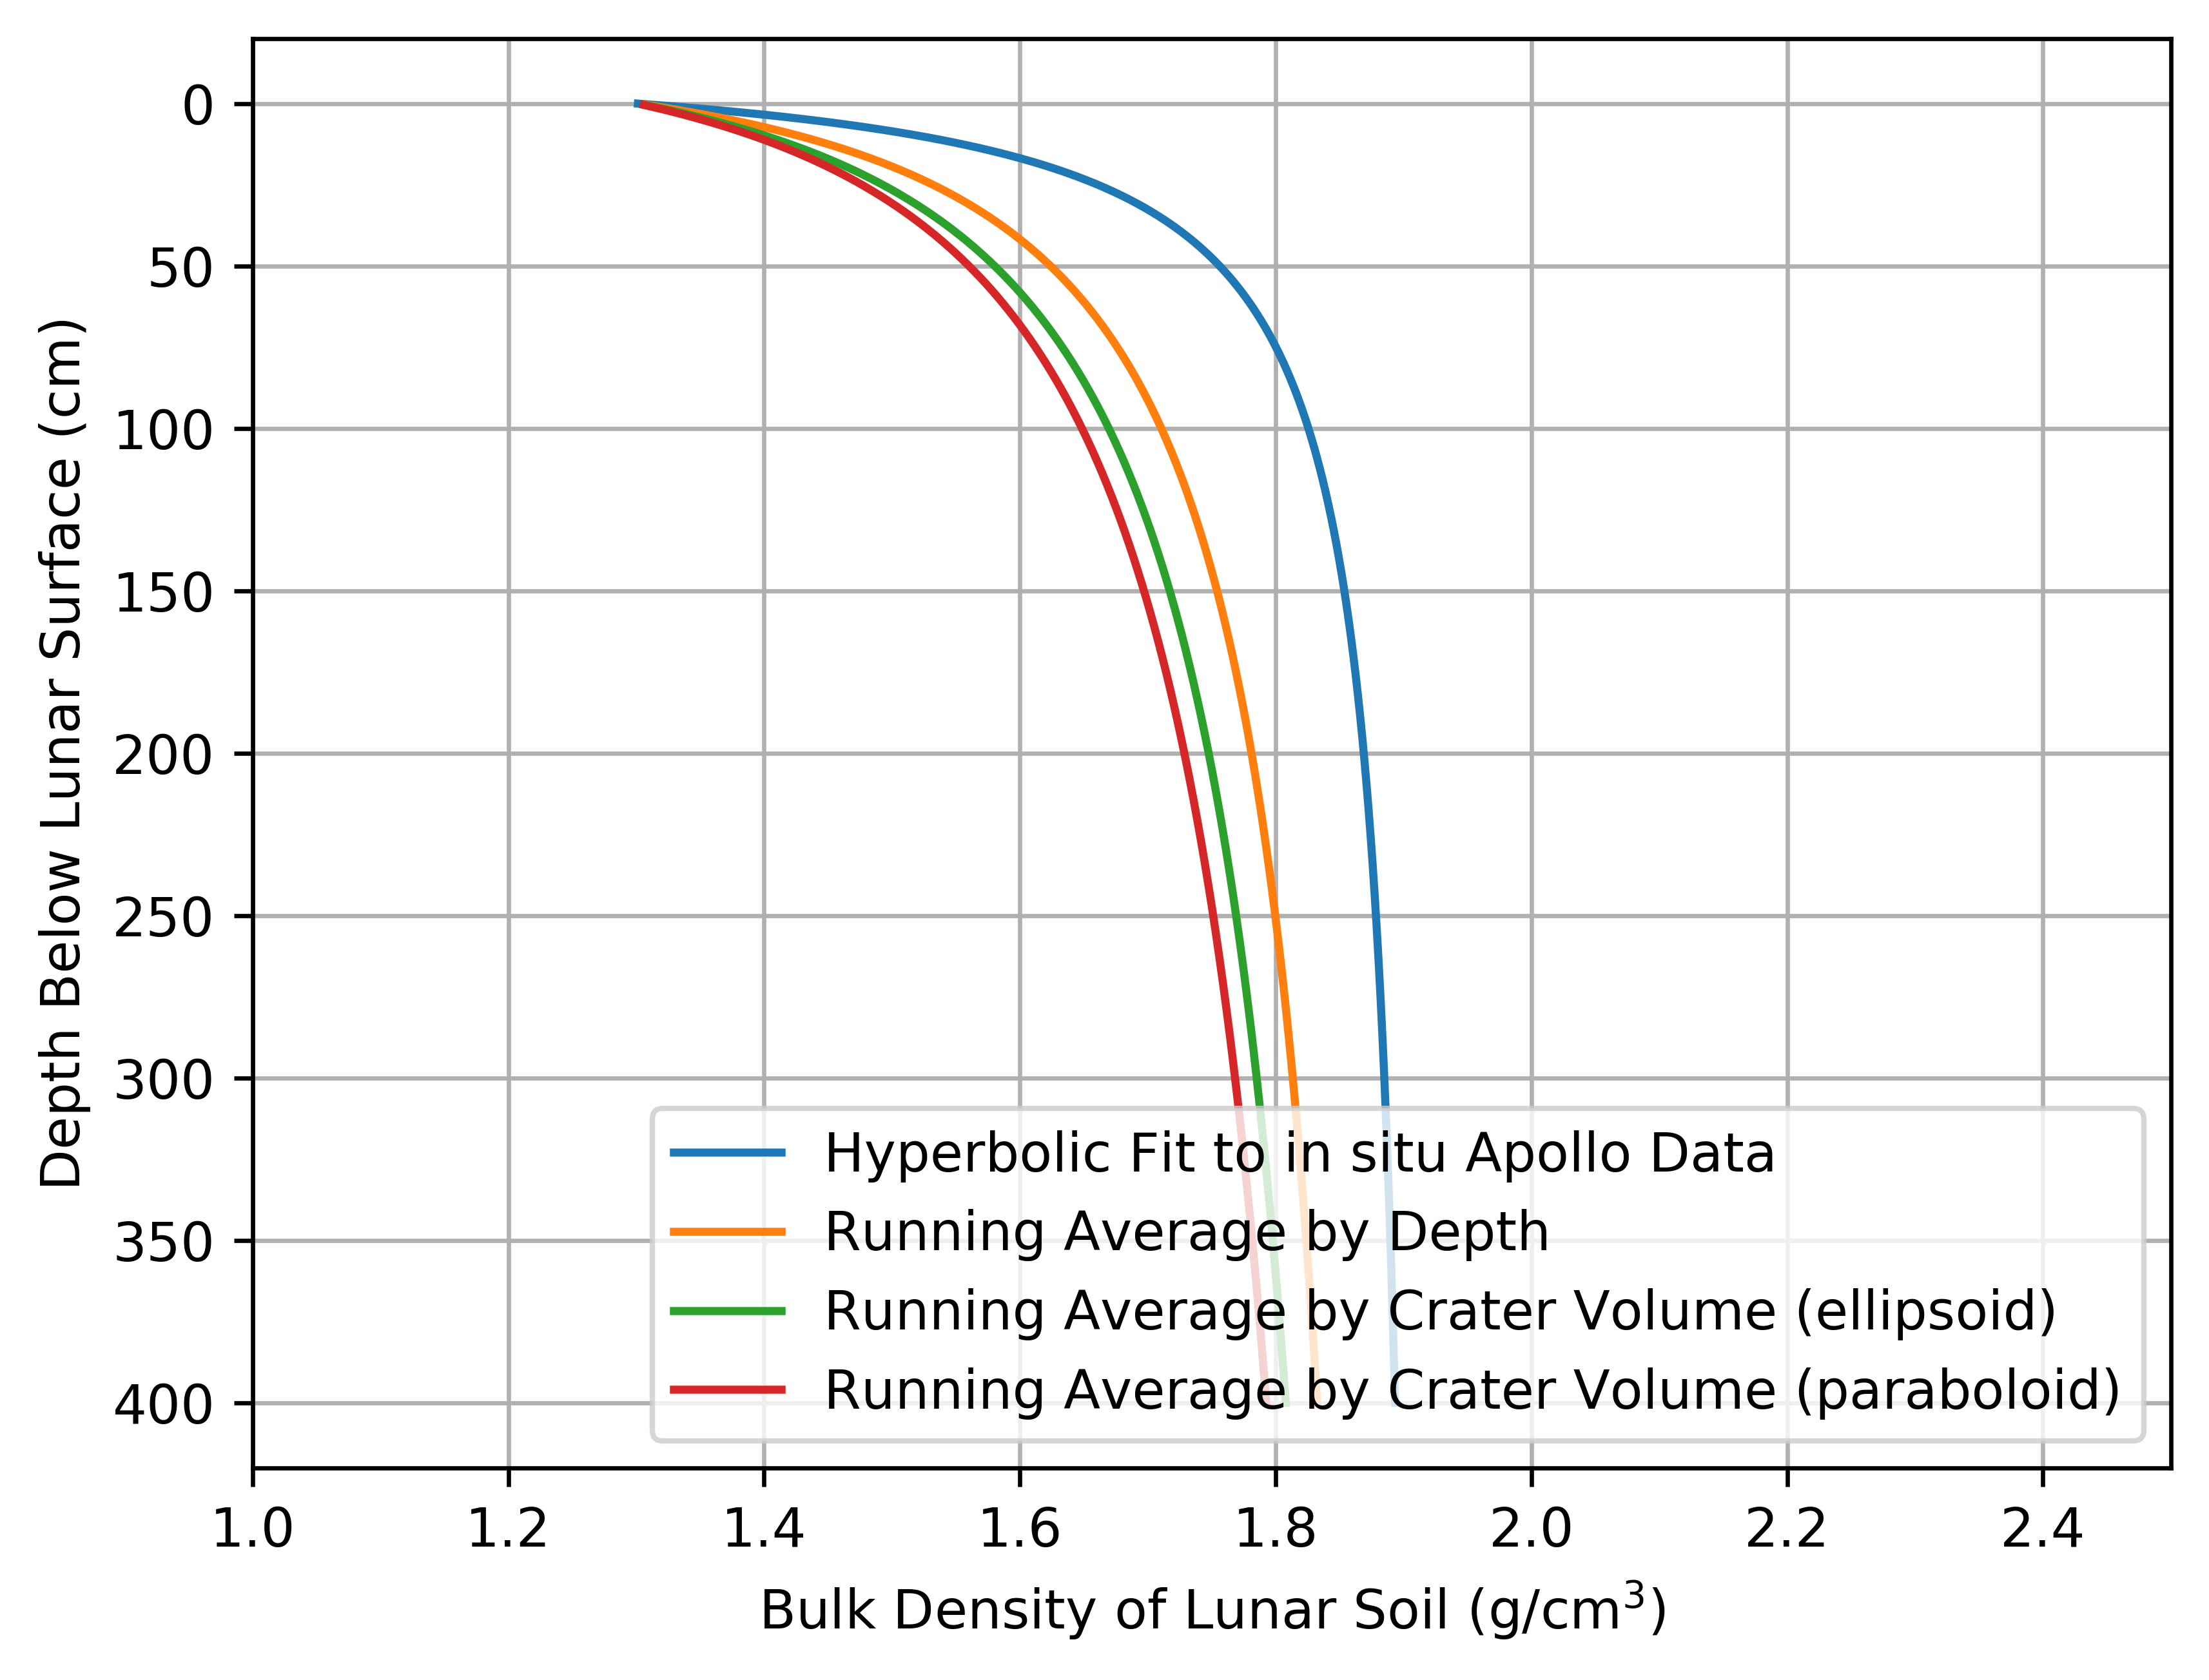
\includegraphics[width=\linewidth]{regolith_density_vs_depth.png}
	\caption{A comparison of the regolith bulk density for a certain depth depth (blue), the depth-averaged bulk density (orange), and the volume-averaged bulk density (green). See also, Figure 9.16 of the Lunar Sourcebook \citep{heiken1991lunar}.}
	\label{fig:regolith_density_vs_depth}
\end{figure}

For a higher-fidelity estimate of the average bulk density sampled by the crater, a volume-average can be used instead of a depth-average, given by
\begin{equation}\label{eq:density volume averaged def}
\rho_{avg, volume}(z) = \frac{\int dV \rho(z')}{\int dV}.
\end{equation}
Expanding the integral in a cylindrical coordinate system and assuming an ellipsoidal crater shape, Equation \eqref{eq:density volume averaged def} becomes
\begin{align}
\rho_{avg, ellipsoid}(z) &= \frac{\int_{0}^{z}\int_{0}^{R\sqrt{1-z'^2/z^2}}\int_{0}^{2\pi}d\phi rdr dz' \rho(z')}{\int_{0}^{z}\int_{0}^{R\sqrt{1-z'^2/z^2}}\int_{0}^{2\pi}d\phi rdr dz'}\\\label{eq:density volume averaged}
&= \frac{1.92}{4z^3}\left[z(6ab - 6b^2 - 3az + 3bz + 4z^2) + 6(a-b)(b^2-z^2)\ln\left(\frac{b}{z + b}\right)\right],
\end{align}
for the volume-averaged density in g/cm$^3$ with $z$ in cm, where $a = 12.2$ and $b = 18$. Following the example from earlier, the average bulk density of the regolith with a depth range of $0$ -- $60$ cm would be $\rho_{avg, ellipsoid}(60)$ = $1.60$ g/cm$^3$, which is $\sim 3\%$ less than $\rho_{avg, depth}(60) = 1.65$ g/cm$^3$.

On the other hand, if a paraboloid crater shape is assumed, Equation \eqref{eq:density volume averaged def} becomes
\begin{align}
\rho_{avg, paraboloid}(z) &= \frac{\int_{0}^{z}\int_{0}^{R\sqrt{1-z'/z}}\int_{0}^{2\pi}d\phi rdr dz' \rho(z')}{\int_{0}^{z}\int_{0}^{R\sqrt{1-z'/z}}\int_{0}^{2\pi}d\phi rdr dz'}\\\label{eq:density volume averaged_para}
&= \frac{1.92}{z/2}\left[b-a + \frac{z}{2} - \frac{(a-b)(b+z)\ln\left(\frac{b}{z+b}\right)}{z}\right],
\end{align}
using the same values for $a$ and $b$ as before. Again, with the prior example, the average bulk density of the regolith with a depth range of $0$ -- $60$ cm would be $\rho_{avg, paraboloid}(60)$ = $1.58$ g/cm$^3$, which is $\sim 4\%$ less than $\rho_{avg, depth}(60) = 1.65$ g/cm$^3$, see Figure \ref{fig:ratio_of_avg_bulk_density}. The expression given in Equation \eqref{eq:density volume averaged_para} is useful for computing the ejected mass from a crater\footnote{In an iterative fashion, since the crater radius depends on the regolith density.}, given a crater depth $z$.





The expressions for the regolith density at a certain depth $z$, weighted by depth, and weighted by crater volume (ellipsoid and paraboloid) are given by Equations \eqref{eq:regolith density vs depth}, \eqref{eq:density depth averaged}, and \eqref{eq:density volume averaged}, \eqref{eq:density volume averaged_para}, respectively, are compared in Figure \ref{fig:regolith_density_vs_depth}. The crater volume is approximated as a half-ellipsoid with two of the dimensions scaled by the crater radius $R$ and one dimension scaled by the crater depth $z$, sliced such that the half-ellipsoid is symmetric about the surface normal for Equation \eqref{eq:density volume averaged}. On the other hand, a paraboloid-shaped crater is used for Equation \eqref{eq:density volume averaged_para}. For a given crater, more of the volume is near the surface so that more weight is given by bulk densities that originate near the surface. In contrast, the depth-averaged bulk density takes the bulk density at each depth equally. This results in the volume-averaged bulk density to be slightly less than the depth-averaged bulk density, as shown in Figure \ref{fig:regolith_density_vs_depth}. In addition, comparing an ellipsoidal crater vs.\ a parabolic crater, the parabolic crater (typically used in literature, see \cite{singer2020lunar}) exhibits the softest increase of the average bulk density as a function of depth.


\begin{figure}[!htb]
	\centering
	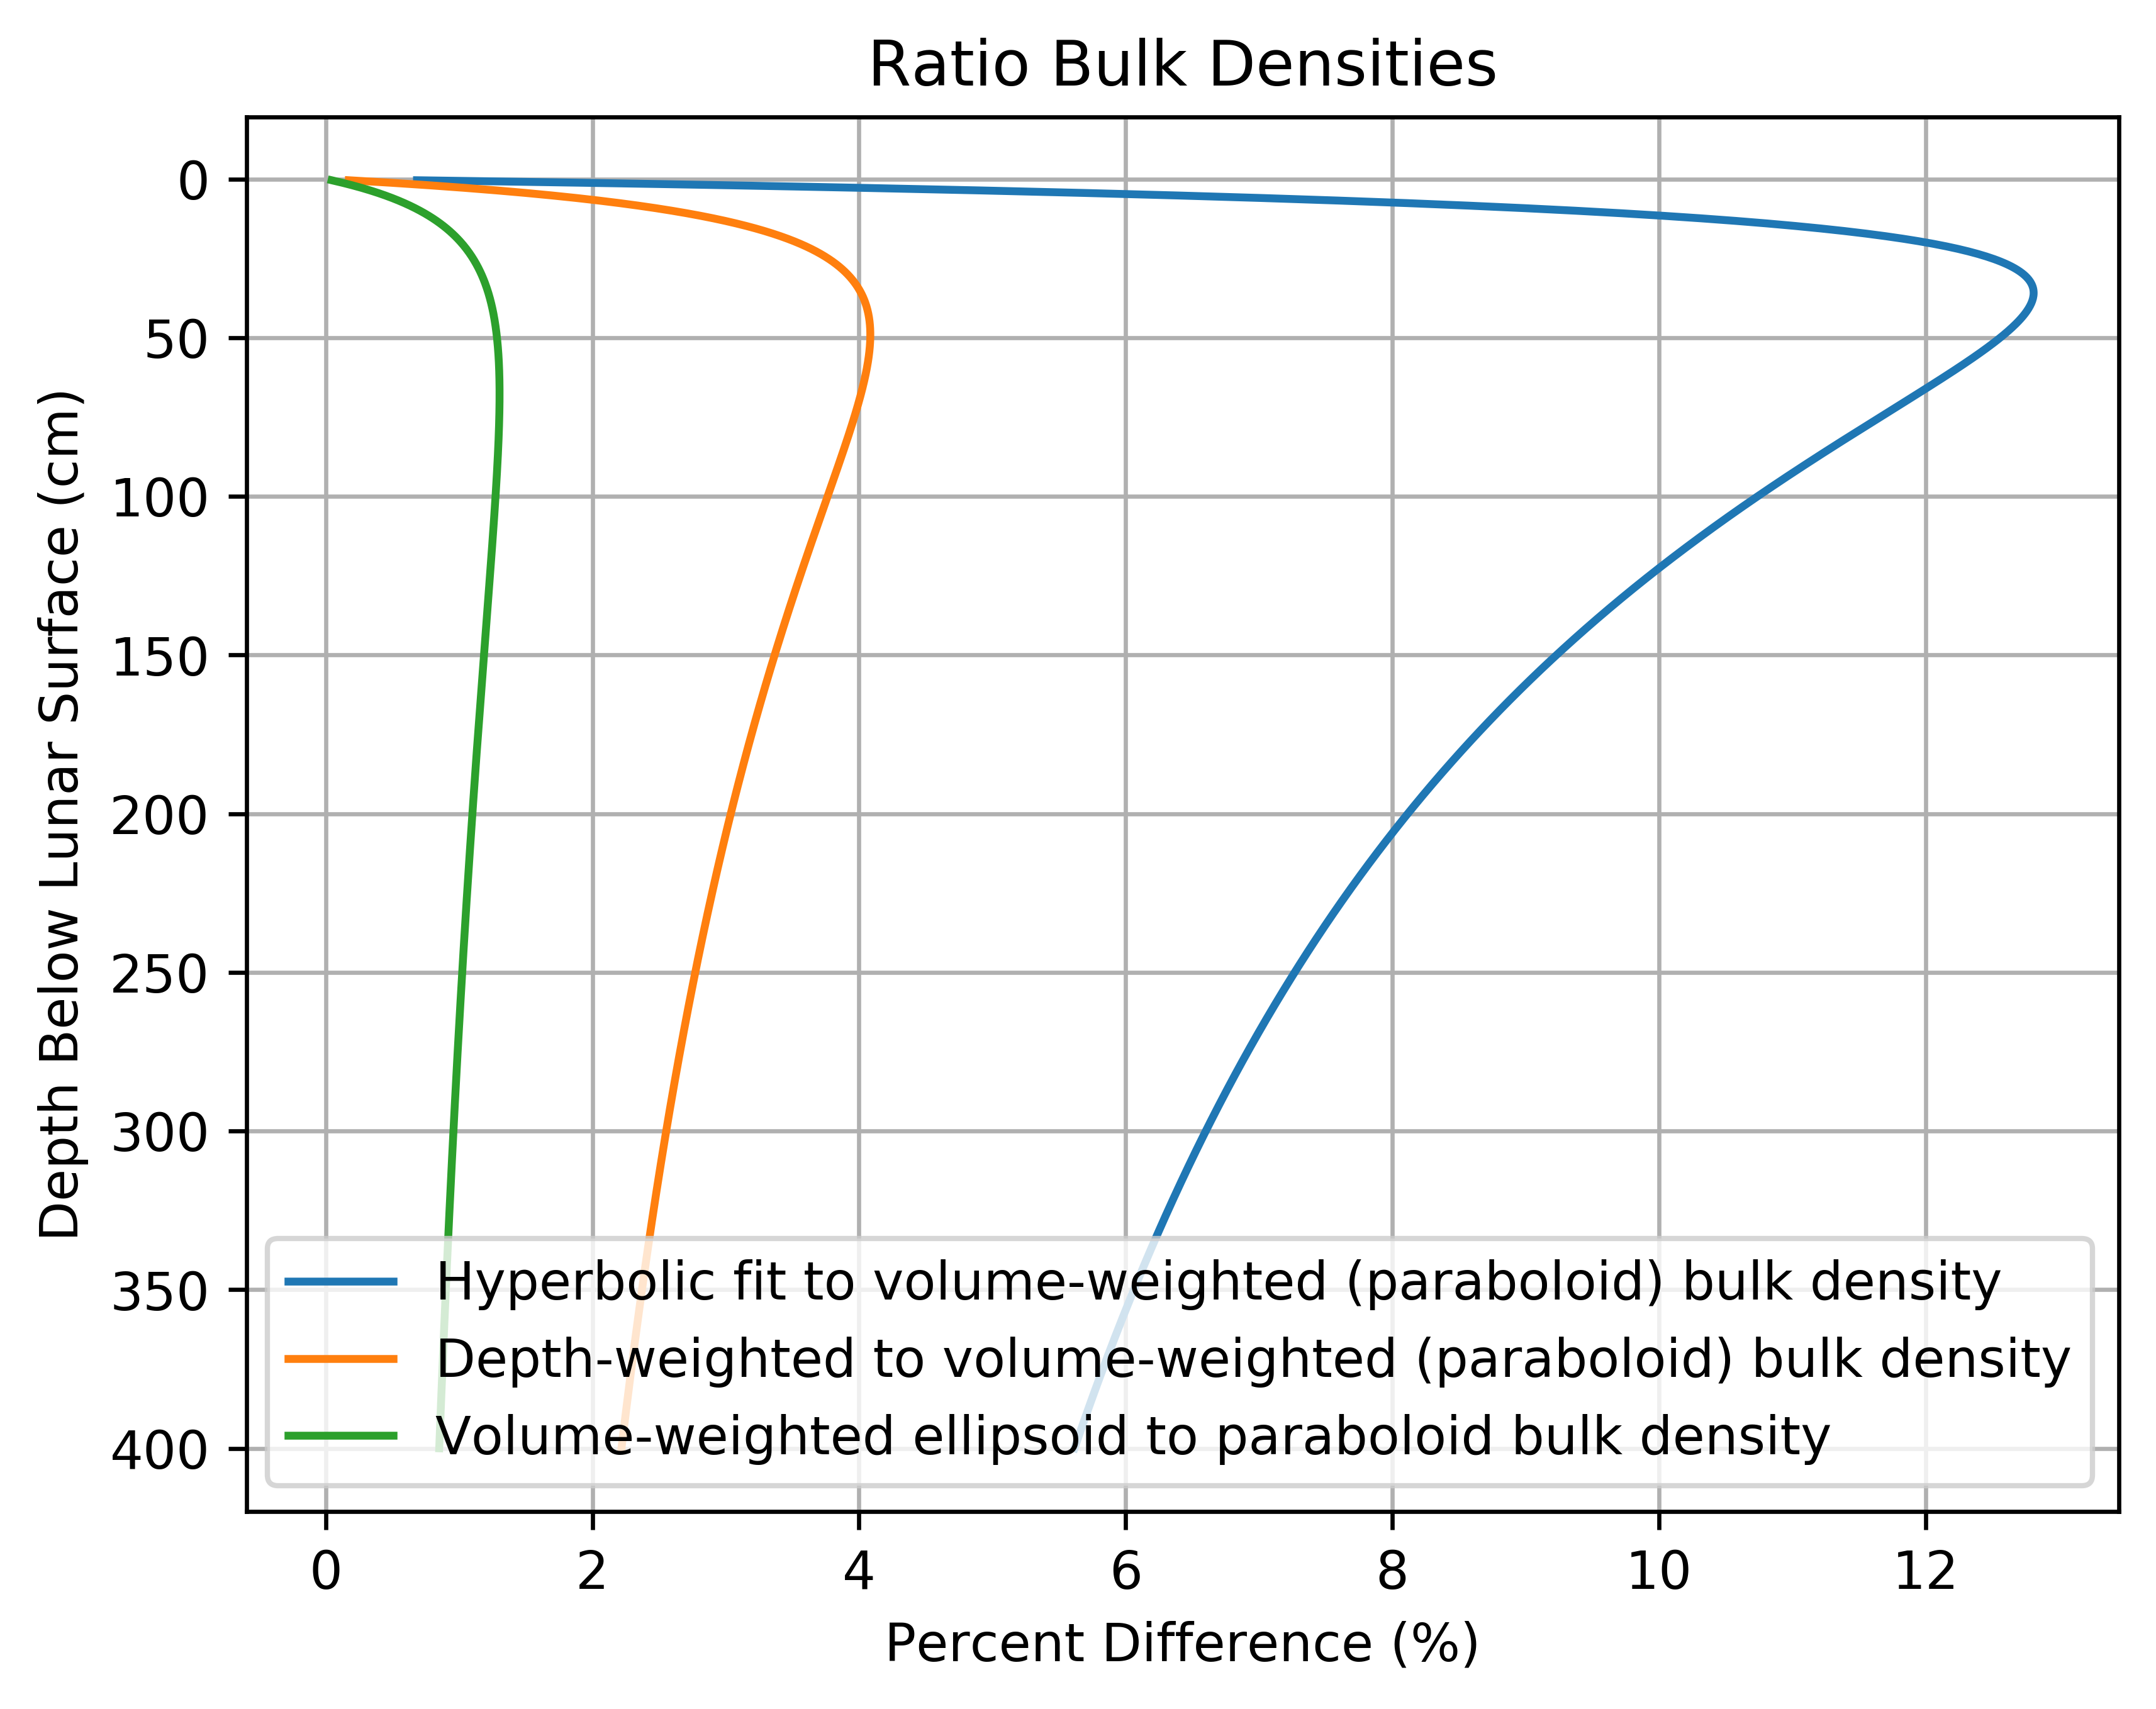
\includegraphics[width=\linewidth]{ratio_of_avg_bulk_density.png}
	\caption{Relative error of using the density at a certain depth (blue) and using the depth-weighted average (orange) of the regolith bulk density.}
	\label{fig:ratio_of_avg_bulk_density}
\end{figure}


%%%%%%%%%%%%%%%%%%%%%%%%%%%%%%%%%%%%%%%%%%%%%%%%%%%%%%%%%%%%%%%%%%%%%%
\subsection{Strength}

The strength of the regolith can be measured in different ways, depending on the use. In the case of modeling impacts, the shear strength of loose regolith and tensile strength of solid rock can be used. The top $10$ m or so consists of fine-grained material called regolith. From $10$ m to about $2$ km is the large scale ejecta that is course grained and ballistically transported (Fig 4.22 of the Lunar Sourcebook, \cite{heiken1991lunar}). All of the impacts studied in this model will create craters less than $2$ km, so it is expected that the shear strength will be used for the loose regolith and large scale ejecta material.

The shear strength of the lunar soil increases with the depth. As an example, both Figure 9.26 of the Lunar Sourcebook, reproduced in Figure \ref{fig:shear_strength_vs_depth}, and Table 12 of \cite{slyuta2014physical} depict this characteristic, shown in Table \ref{tab:shear_strength}.

\begin{table}[!htb]
	\begin{center}
		\caption{The change of the shear strength of the lunar soil with depth.}
		\label{tab:shear_strength}
		\begin{tabular}{c c}
			\hline
			Depth (cm)  & Shear strength (kPa)  \\
			\hline
			$5$  & $0.1$ -- $2.5$  \\
			$50$  & $1$ -- $3.5$   \\
			$100$ & $2$ -- $4$  \\
			$200$  & $4$ -- $8$  \\\hline
		\end{tabular}
	\end{center}
\end{table}

\begin{figure}[!htb]
	\centering
	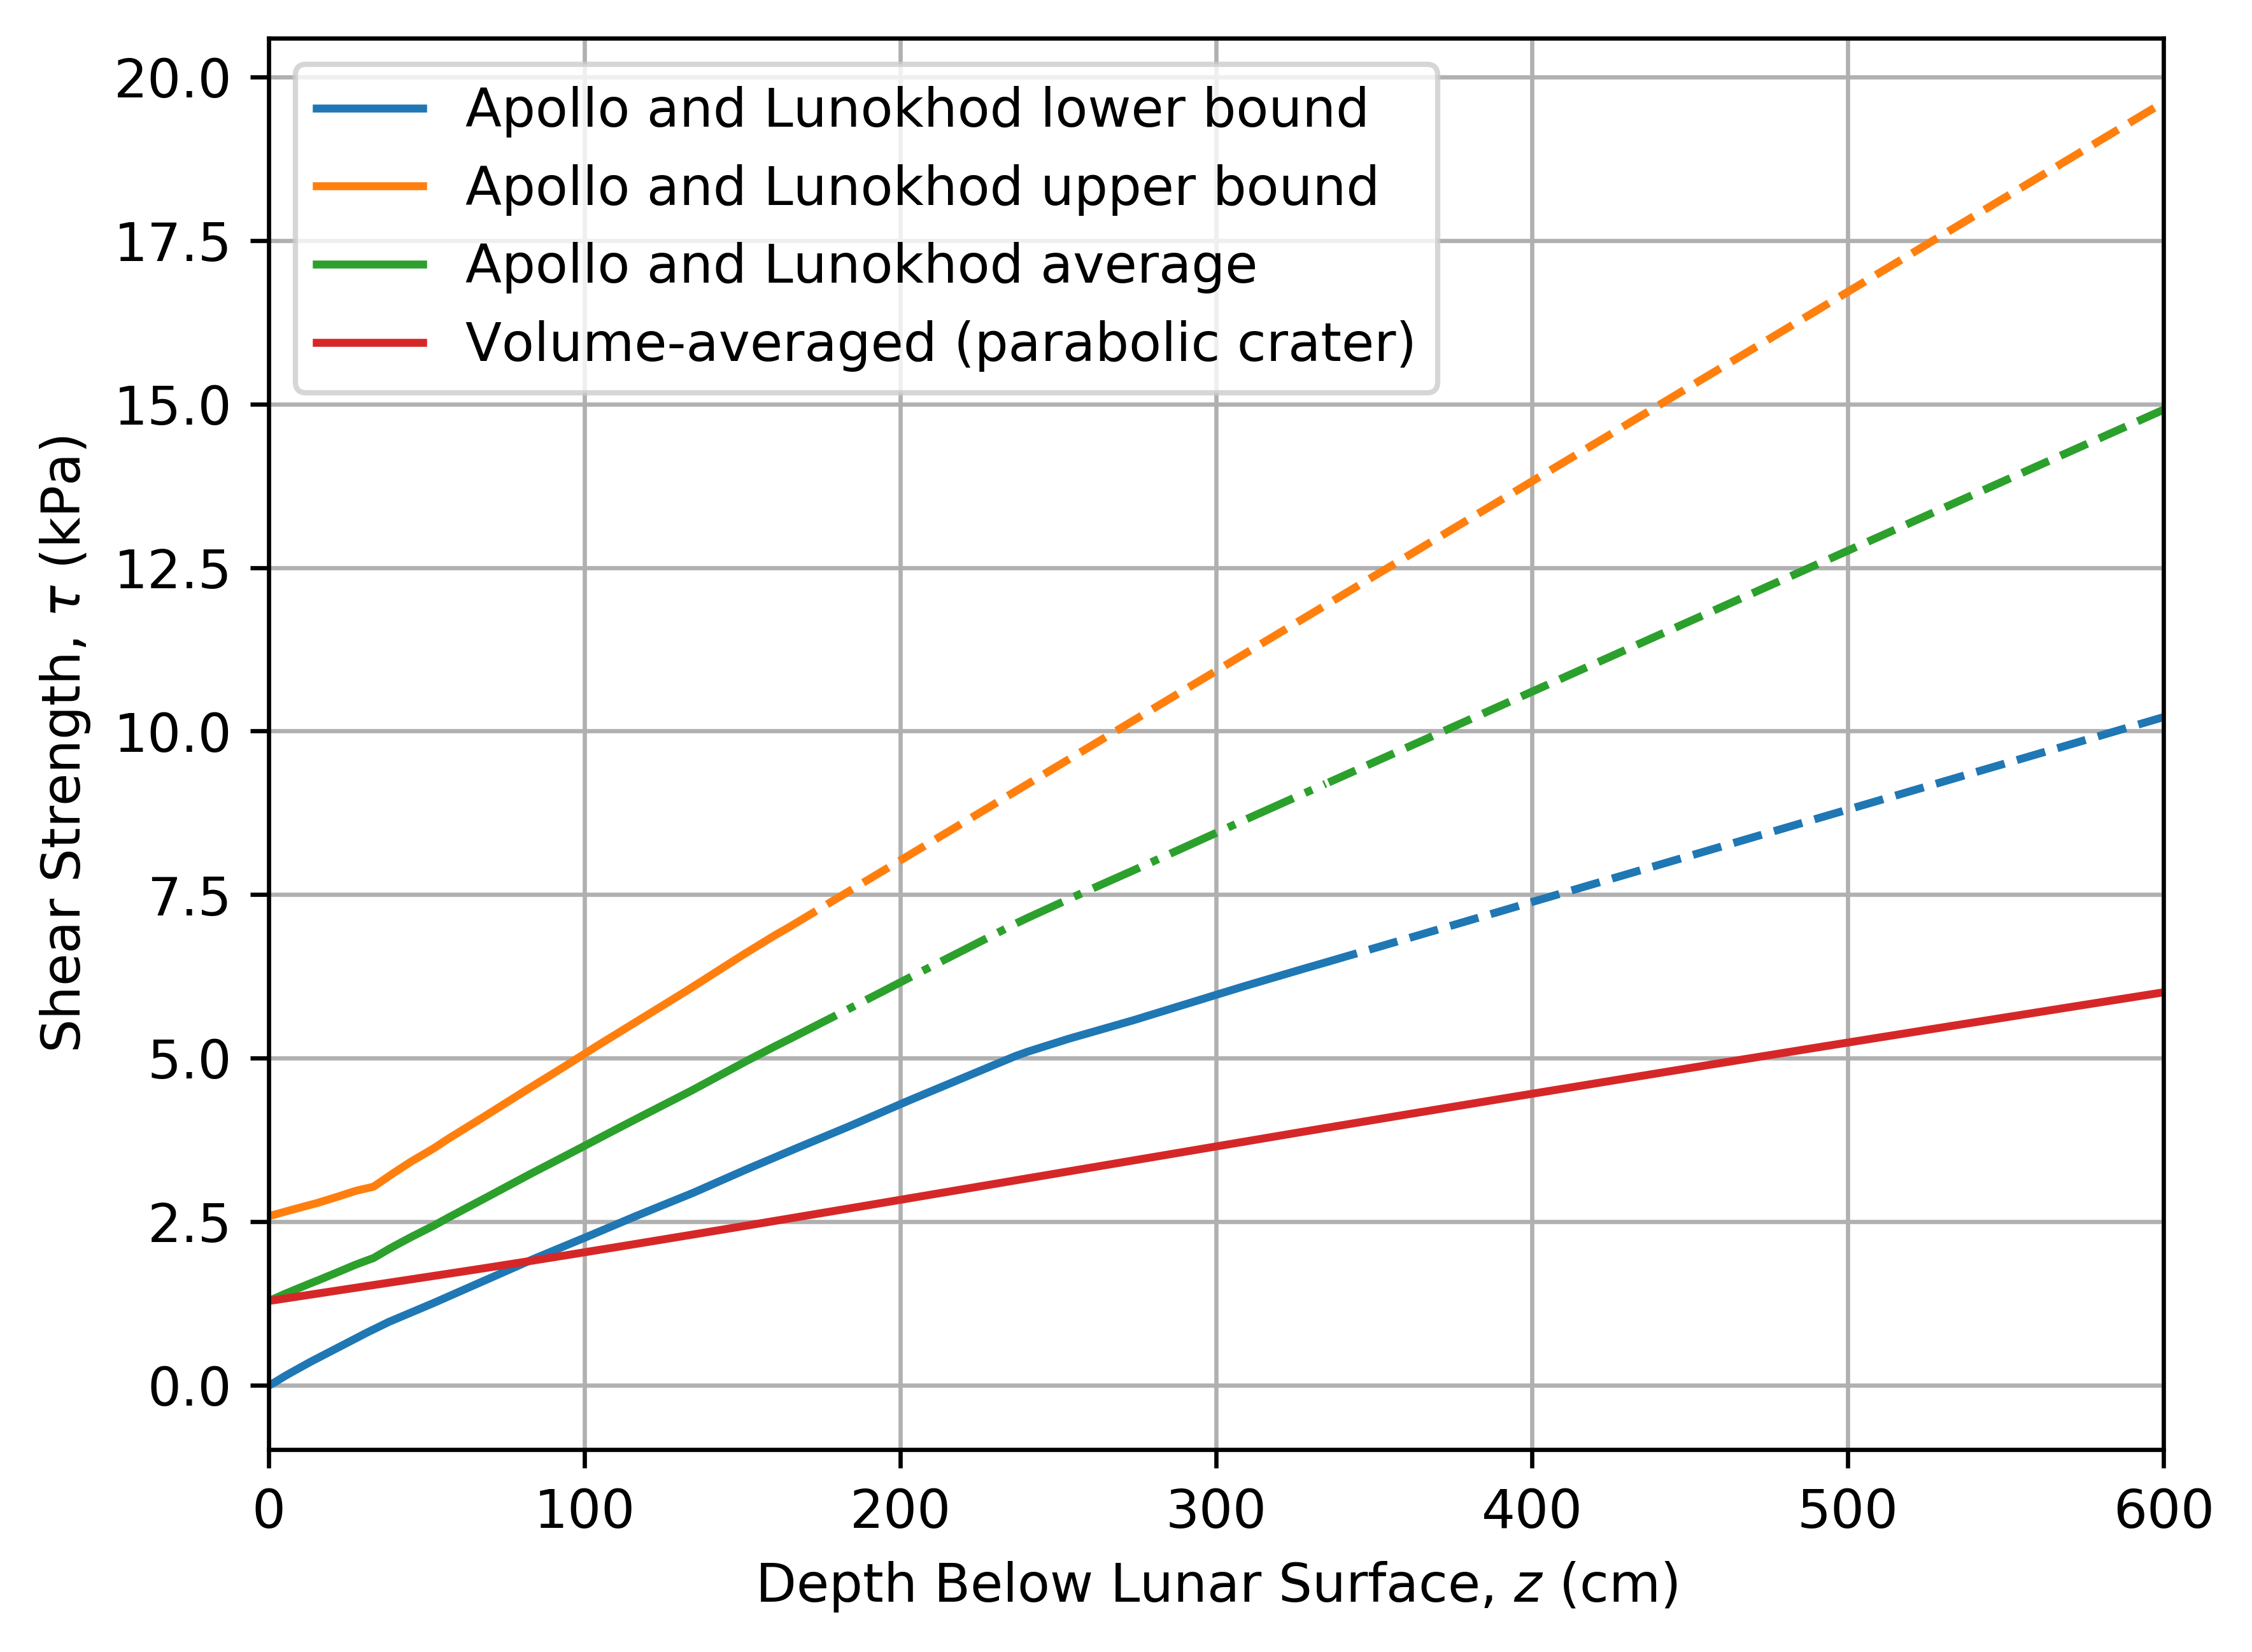
\includegraphics[width=\linewidth]{shear_strength_vs_depth.png}
	\caption{The range of regolith shear strength as a function of depth below the lunar surface taken from Figure 9.26 of the Lunar Sourcebook. The average shear strength is also calculated (green). Points that are extrapolated beyond what is available are shown by the dashed lines. The volume-averaged shear strength (red) assumes a parabolic-shaped crater of depth $z$.}
	\label{fig:shear_strength_vs_depth}
\end{figure}

The average shear strength (green curve) in Figure \ref{fig:shear_strength_vs_depth} can be expressed by the piece-wise form
\begin{equation}\label{eq:shear strength}
\tau(z) =
\begin{cases}
\frac{z}{45.55} + 1.288,\text{   $0 \le z < 50$ cm}\\
\frac{z}{40.21} + 1.144,\text{   $50$ cm $\le z < 250$ cm}\\
\frac{z}{46.06} + 1.942,\text{   $z > 250$ cm}
\end{cases}.
\end{equation}
Assuming the crater has a parabolic shape and that the effective shear strength is the volume-average, Equation \eqref{eq:shear strength} becomes (as shown by the red curve in Figure \ref{fig:shear_strength_vs_depth})
\begin{equation}\label{eq:shear strength_avg_para}
\tau(z) =
\begin{cases}
\frac{z}{136.65} + 1.288,\text{   $0 \le z < 50$ cm}\\
\frac{z}{120.63} + 1.144 + \frac{7.163}{z} - \frac{118.33}{z^2},\text{   $50$ cm $\le z < 250$ cm}\\
\frac{z}{138.18} + 1.942 - \frac{194.81}{z} + \frac{16902}{z^2},\text{   $z > 250$ cm}
\end{cases}.
\end{equation}



%%%%%%%%%%%%%%%%%%%%%%%%%%%%%%%%%%%%%%%%%%%%%%%%%%%%%%%%%%%%%%%%%%%%%%
\subsection{Particle Size Distribution}


%%%%%%%%%%%%%%%%%%%%%%%%%%%%%%%%%%%%%%%%%%%%%%%%%%%%%%%%%%%%%%%%%%%%%%
\subsection{Scaling Law Properties}



\end{document}
\documentclass{article}
\usepackage{amsmath}
\usepackage{graphicx}

\begin{document}
\section{Primary Flux Environment}



%%%%%%%%%%%%%%%%%%%%%%%%%%%%%%%%%%%%%%%%%%%%%%%%%%%%%%%%%%%%%%%%%%%%%%
\subsection{Space-Time Dependence of Environment}


%%%%%%%%%%%%%%%%%%%%%%%%%%%%%%%%%%%%%%%%%%%%%%%%%%%%%%%%%%%%%%%%%%%%%%
\subsubsection{Ephemeris Definition}


%%%%%%%%%%%%%%%%%%%%%%%%%%%%%%%%%%%%%%%%%%%%%%%%%%%%%%%%%%%%%%%%%%%%%%
\subsubsection{Selenographic Extent}


%%%%%%%%%%%%%%%%%%%%%%%%%%%%%%%%%%%%%%%%%%%%%%%%%%%%%%%%%%%%%%%%%%%%%%
\subsection{Sporadic Meteoroid Complex}
	
%%%%%%%%%%%%%%%%%%%%%%%%%%%%%%%%%%%%%%%%%%%%%%%%%%%%%%%%%%%%%%%%%%%%%%
\subsection{Near-Earth Objects}

%%%%%%%%%%%%%%%%%%%%%%%%%%%%%%%%%%%%%%%%%%%%%%%%%%%%%%%%%%%%%%%%%%%%%%
\subsection{Meteoroid Showers}

	
\end{document}
\documentclass{article}
\usepackage{amsmath}
\usepackage{graphicx}

\begin{document}
\section{Ejecta Flux from Impact Point}\label{sec:Secondary Flux Environment}

The ejected mass from an impact is distributed at different speeds (Section \ref{sssec:Ejecta:Speed Distribution}), angles (Sections  \ref{sssec:Ejecta:Zenith Distribution} and \ref{sssec:Ejecta:Azimuth Distribution}), and sizes (Section \ref{ssec:Mass/Particle Size Distribution}). The speed and size of the ejecta is assumed to be dependent on each other -- the larger the ejected particle the slower, on average, the particle that is ejected. The impactor impact angle and azimuth determines the zenith and azimuth distribution of the ejecta. For more oblique impacts, the ejecta is projected less from normal and more towards the horizon, in addition to having a stronger component downstream with respect to the impactor azimuth in terms of the ejecta azimuth distribution. 



%%%%%%%%%%%%%%%%%%%%%%%%%%%%%%%%%%%%%%%%%%%%%%%%%%%%%%%%%%%%%%%%%%%%%%
\subsection{Ejecta Distribution}\label{ssec:Ejecta Distribution}




%%%%%%%%%%%%%%%%%%%%%%%%%%%%%%%%%%%%%%%%%%%%%%%%%%%%%%%%%%%%%%%%%%%%%%
\subsubsection{Speed Distribution}\label{sssec:Ejecta:Speed Distribution}

The speed distribution of the ejecta is determined by the scaling laws \citep{housen2011ejecta} that are assumed in this model (see Section \ref{sec:Scaling Laws}). As an approximation, the speed distribution can be described by a power-law distribution with an index that depends on the target material. However, a more complete speed distribution is used that not only includes a power-law regime, but includes proper cut-offs for the slowest speeds and fastest speeds.%, discussed in Section \ref{ssec:Min Max Ejecta Speed}.


%%%%%%%%%%%%%%%%%%%%%%%%%%%%%%%%%%%%%%%%%%%%%%%%%%%%%%%%%%%%%%%%%%%%%%
\subsubsection{Zenith Distribution}\label{sssec:Ejecta:Zenith Distribution}

The ejecta zenith distribution is typically peaked at some zenith angle $\alpha_{max}$ that falls off at other angles. The peak zenith angle $\alpha_{max}$ can have different dependencies on the impactor properties.


\paragraph{Constant Zenith Peak:}
The simplest case is a constant, $\alpha_{max} = \alpha_0$, typically taken as $\alpha_0 = \pi/4$. For relatively close impact distances, an ejected angle of $45^\circ$ gives the most efficient ejecta -- the ejecta travels further for a given speed.

\paragraph{Impact Angle Dependent Zenith Peak:}
To include more information into the ejecta blanket from the impactor is to have the zenith peak as a function of the impact angle, $\alpha_{max} = \alpha_{max}(\alpha_i)$, where $\alpha_i$ is the impact angle of the impactor. For simplicity, the peak zenith angle can be taken as the downstream for all azimuth, given in Equation~\eqref{eq:peak zenith downstream}.

\paragraph{Impact Angle \& Azimuth Dependent Zenith Peak:}
An increased fidelity peak zenith angle also include information about the impactor azimuth angle, $\alpha_{max} = \alpha_{max}(\alpha_i, \beta_i)$, where $\beta_i$ is the impact azimuth.

The peak zenith angle can be modeled after experiments of oblique impacts following Figure~18 of \cite{gault1978experimental} as a proxy to the model of $\alpha_{max}$. Using a third-order polynomial for both fits to the downstream and upstream angles given in Table \ref{tab:upstream_downstream_angles}, the peak zenith angles downstream and upstream are given by
\begin{align}\label{eq:peak zenith downstream}
\alpha_{max}(\beta - \beta_i = 0) &= 0.0003\alpha_i^3 - 0.036\alpha_i^2 + 1.5206\alpha_i + 20, \text{ downstream}\\
\alpha_{max}(\beta - \beta_i = \pi) &= -0.00042\alpha_i^3 + 0.0236\alpha_i^2 + 0.129\alpha_i + 20, \text{ upstream}
\end{align}
in units of degrees, where $\beta$ is the ejecta azimuth. When both the impact and ejecta azimuth angles are in the same direction (i.e., $\beta-\beta_i = 0$), this is downstream.

\begin{table}[h]\centering
	\caption{Cone angles of upstream and downstream of impact derived from Figure 18 of \cite{gault1978experimental}.}\label{tab:upstream_downstream_angles}
	\begin{tabular}{|c | c | c |}\hline
		Impact Zenith Angle & Upstream Zenith Angle & Downstream Zenith Angle\\\hline
		0	&20	&20\\\hline
		15	&24	&35\\\hline
		30	&35	&45\\\hline
		45	&28	&40\\\hline
		60	&13	&54\\\hline
		75	&-35	&66\\\hline		
	\end{tabular}
\end{table}


\paragraph{Rival \& Mandeville (Gaussian Distribution):}
One example of a peaked distribution is given in \cite{rival1999modeling}, shown below for reference:
\begin{equation}\label{eq:Rival_zenith-dist}
F(\alpha) = \frac{1}{\sigma\sqrt{2\pi}}\exp\left[-\frac{(\alpha-\alpha_{max})^2}{2\sigma^2}\right],
\end{equation}
where $\alpha_{max}$ is defined as
\begin{equation}
\alpha_{max} = 
\begin{cases}
\frac{\alpha_{max60}-\alpha_{max0}}{\pi/3}\alpha_i + \alpha_{max0}\text{  for $\alpha_i\le \pi/3 = 60^\circ$}\\
\alpha_{max60}\text{  for $\alpha_i > \pi/3 = 60^\circ$}
\end{cases},
\end{equation}
for $\alpha_i$ the impact zenith angle, and \citep[see][]{ESABASE2_DebrisRelease10.0}
\begin{align}
\alpha_{max0} &= \frac{\pi}{6} = 30^\circ,\\
\alpha_{max60} &= \frac{4\pi}{9} = 80^\circ,\\
\sigma &= \frac{\pi}{60} = 3^\circ,
\end{align}
where the peak ejecta angle is shifted from $30^\circ$ of zenith for a normal impact to $80^\circ$ of zenith for oblique impacts ($>60^\circ$).

One difficulty with this zenith distribution is the normalization, assuming ejecta is only created from $0 < \alpha < \pi/2 $. A Gaussian distribution is usually integrated from $-\infty$ to $+\infty$, so a finite integration introduces error functions.

\paragraph{Raised Cosine Distribution:}
A more focused zenith distribution that is easier to normalize can be described by a raised cosine distribution, given as
\begin{equation}\label{eq:zenith-rasied cosine dist}
F(\alpha) = \begin{cases}
\frac{1}{2s}\left[1 + \cos\left(\frac{\alpha-\mu}{s}\pi\right)\right] \text{, for $\mu-s \le \alpha \le \mu+s$}\\
0 \text{, otherwise}
\end{cases},
\end{equation}
This distribution is symmetric about the peak $\mu$, with a spread $s$. It is assumed that $\mu-s \ge 0$ and $\mu+s \le \pi/2$, otherwise the normalization term would be dependent on the peak, in addition to the spread.

%%%%%%%%%%%%%%%%%%%%%%%%%%%%%%%%%%%%%%%%%%%%%%%%%%%%%%%%%%%%%%%%%%%%%%
\subsubsection{Azimuth Distribution}\label{sssec:Ejecta:Azimuth Distribution}

The azimuth distribution is often dependent on the impactor azimuth such that there are more ejecta downstream for oblique impacts. Normal impacts are expected to produce a symmetric azimuth distribution. For highly oblique impacts ($\alpha_i > \pi/3$) there is often seen a \textit{butterfly pattern} \citep{shuvalov2011ejecta}. However, over a large number of oblique impacts of various sizes, it is plausible to assume that the direct downstream direction dominates the azimuth distribution.

\paragraph{Rival \& Mandeville:}
An example azimuth distribution can be found in \cite{rival1999modeling}, given by
\begin{equation}\label{eq:azm_rival_mandeville}
G(\beta) =
\begin{cases}
\frac{1}{2\pi}\left[1+\frac{3\alpha_i}{2\pi - 3\alpha_i}\cos(\beta-\beta_i)\right] \text{  for $\alpha_i\le \pi/3 = 60^\circ$}\\
\frac{1}{\sigma'\sqrt{2\pi}}\exp\left[-\frac{(\beta-\beta_i)^2}{2\sigma'^2}\right]
\text{  for $\alpha_i > \pi/3 = 60^\circ$}
\end{cases},
\end{equation}
where
\begin{equation}
\sigma' = \frac{\pi}{36} = 5^\circ, 
\end{equation}
for $\beta_i$ the impact azimuth angle + $\pi$.

\paragraph{Variation on Rival \& Mandeville:} In order to have a periodic and easy-to-normalize function, the oblique regime is modified from Equation \eqref{eq:azm_rival_mandeville} to give
\begin{equation}\label{eq:azm_mod_rival_mandeville}
G(\beta) =
\begin{cases}
\frac{1}{2\pi}\left[1+\frac{3\alpha_i}{2\pi - 3\alpha_i}\cos(\beta-\beta_i)\right] \text{  for $\alpha_i\le \pi/3 = 60^\circ$}\\
\frac{1 + \cos(\beta-\beta_i)}{2\pi}
\text{  for $\alpha_i > \pi/3 = 60^\circ$}
\end{cases}.
\end{equation}

An alteration of Equation \eqref{eq:azm_mod_rival_mandeville} on the oblique case could be to use a raised cosine distribution with a spread of $ s = 3\sigma'$.




%%%%%%%%%%%%%%%%%%%%%%%%%%%%%%%%%%%%%%%%%%%%%%%%%%%%%%%%%%%%%%%%%%%%%%
\subsection{Mass/Particle Size Distribution}\label{ssec:Mass/Particle Size Distribution}

The mass or particle size distribution of ejecta can be approximated in a few different ways. For the purpose of comparing to various sources, there are four possible ways to describe the particle size distribution, give by \citep{koschny2001impacts_mass}
\begin{align}
m_{cum}(\le d) &= k_1 d^\alpha,\label{eq:KG01 m_cum d}\\
N_{cum}(\ge m) &= k_2 m^{-\beta},\label{eq:KG01 N_cum m}\\
N_{cum}(\ge d) &= k_3 d^\gamma,\label{eq:KG01 N_cum d}\\
m_{cum}(\le m) &= k_4 m^\delta,\label{eq:KG01 m_cum m}
\end{align}
with $N_{cum}$ the cumulative number, $m_{cum}$ the cumulative mass, $d$ the particle diameter, and $m$ the particle mass.

The various transformations between the four possible descriptions are:
\begin{align}
\beta &= -\gamma/3,\\
\alpha &= 3(1-\beta),\\
\alpha &= \gamma + 3,\\
\delta &= \alpha/3.
\end{align}

Table IV of \citep{koschny2001impacts_mass} gives examples of the exponent $\alpha$, summarized here in Table \ref{tab:mass-diameter_index_examples}.

\begin{table}[!htb]
	\begin{center}
	\caption{A compilation of indices of the various particle size distribution descriptions. Values that are in bold are the index that was originally used in the corresponding source.}\label{tab:mass-diameter_index_examples}
	\begin{tabular}{|c | c | c | c | c|}\hline
		\textbf{Target Material} & \textbf{Source} & $\alpha$ & $\beta$ & $-\gamma$ \\\hline
		Basalt	& \cite{koschny2001impacts_mass}	& \textbf{0.56, 0.96} & 0.81, 0.68 & 2.44, 2.04\\\hline
		Granite	& ''	&\textbf{ 0.44} & 0.85 & 2.56\\\hline
		Gabbro	& ''	& \textbf{1.41} & 0.53 & 1.59\\\hline
		Alumina	& ''	& \textbf{1.08} & 0.64 & 1.92\\\hline
		Water ice	& ''	& \textbf{1.3} & 0.57 & 1.7\\\hline
		Porous ice-silicate	& ''	& \textbf{1.8} & 0.4 & 1.2\\\hline
		Compact ice-silicate	& ''	& \textbf{1.4$\pm$0.3} & 0.53$\pm$0.1 & 1.6$\pm$0.3\\\hline
		Basalt & \cite{cour1969meteoroid} & -0.6 & \textbf{1.2} & 3.6\\\hline
		Sandstone & \cite{buhl2014ejecta} & 0.26-0.46 & 0.85-0.91 & \textbf{2.54-2.74} \\\hline
		Apollo Samples & \cite{carrier2003particle} & -0.55 & 1.18 & \textbf{3.55}$^a$ \\\hline
		Basalt + others & \cite{oKeefe1985impact} & \textbf{0.42-0.53} & 0.82-0.86 & 2.47-2.58 \\\hline
		\multicolumn{5}{l}{\footnotesize $^a$ valid for diameters from $10^{-6}$ m to $10^{-1}$ m.}
	\end{tabular}
\end{center}
\end{table}


\subsubsection{NASA SP-8013}
The Meteoroid Environment Model - 1969 Near Earth to Lunar Surface \citep{cour1969meteoroid}, or NASA SP-8013, contains both the primary meteoroid environment as well as the lunar ejecta environment. The latter is given in terms of cumulative number flux of secondary ejecta greater than mass $m$ (i.e., in the form of Equation \eqref{eq:KG01 N_cum m}), shown in Figure \ref{fig:NASA-SP-8013-Fig10-flux-mass-distribution} (Figure 10 of \cite{cour1969meteoroid}).


\begin{figure}[!htb]
	\centering
	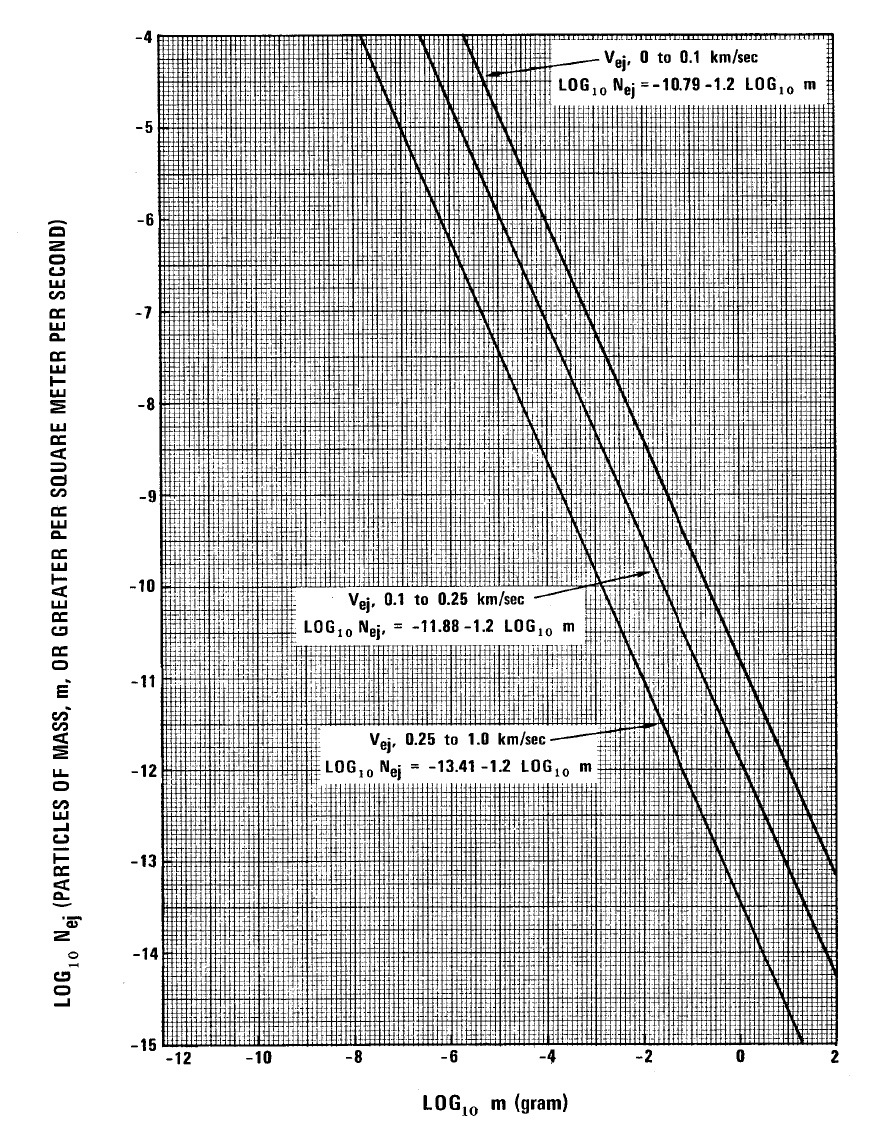
\includegraphics[width=1.0\linewidth]{NASA-SP-8013-Fig10-flux-mass-distribution.PNG}
	\caption{Average cumulative lunar ejecta flux-mass distribution for each of three ejecta velocity intervals \citep{cour1969meteoroid}.}\label{fig:NASA-SP-8013-Fig10-flux-mass-distribution}
\end{figure}

Each of the three velocity intervals have a power-law index of $-\beta = -1.2$, corresponding to $\alpha=-0.6$ (see Table \ref{tab:mass-diameter_index_examples}). Qualitatively, the larger the power-law index $\alpha$ is, the greater number of larger particles are present in the size distribution \citep[e.g.,][]{koschny2001impacts_mass,bierhaus2018secondary}. For a negative $\alpha$, this implies an absence of larger sized particles in the SP-8013 model compared to what is shown in \cite{koschny2001impacts_mass}.

The power-law index of $-\beta = -1.2$ is a simplification of \cite{zook1967problem}, which is what the SP-8013 is based on for lunar ejecta. Figure 5 of \cite{zook1967problem} displays three different velocity ranges with $\beta = 1$ for $0 \le v \le 100$ m/s, $\beta = 1$ for $100 \le v \le 250$ m/s, and $\beta = 1.16$ for $250 \le v \le 1000$ m/s.

It is interesting to point out that the particle size distribution shown in Figure \ref{fig:NASA-SP-8013-Fig10-flux-mass-distribution} has a similar power-law index with the regolith particle size distribution of diameters from $10^{-6}$ m to $10^{-1}$ m of \cite{carrier2003particle}, see Table \ref{tab:mass-diameter_index_examples}. Since the regolith particle size distribution is a log-normal distribution, the power-law index for larger diameters will be even more steep, and therefore a more negative $\alpha$, meaning there is an absence of larger stones or boulders in the top layers of regolith sampled from Apollo.

\subsubsection{O'Keefe \& Ahrens 1985}
A conclusion from \cite{sachse2015correlation} states that \textit{the assumption that the size of the fragments and the speed at the moment of ejection are uncorrelated} should be dropped. In practice, larger ejected particles typically have slower speeds while smaller ejected particles have faster speeds. This observation is not seen in the previous size distribution model of NASA SP-8013\footnote{It is important to note that \cite{zook1967problem} did include a speed dependent size distribution in their model (they looked at three variations, ultimately using a piece-wise power-law model), however, \cite{cour1969meteoroid} in SP-8013 simplified the size distribution to be constant for each of the speed ranges.}, so another model is sought after.

The particle size distribution discussed in \cite{oKeefe1985impact} gives a way to introduce a speed-dependent particle size distribution. The cumulative amount of mass of ejecta fragments of mass greater than $m$ is given by (Equation (11) of \cite{oKeefe1985impact}), note $\beta_{OK85} \equiv \alpha$ as in Table \ref{tab:mass-diameter_index_examples},
\begin{equation}
f(m, m_{bv}(v)) = 1 - \left(\frac{m}{m_{bv}}\right)^{\frac{\beta_{OK85}}{3}},
\end{equation}
where the mass of the largest fragment ejected at a given ejected velocity $v$ is
\begin{equation}
\frac{m_{bv}(v)}{m_b} = \left(\frac{v}{v_{min}}\right)^{-\delta_{OK85}}.
\end{equation}
The speed index $\delta_{OK85}$ is related to the power-law index of the CDF of mass exceeding a certain speed of ejecta (e.g., $3\mu$ from \cite{housen2011ejecta}) and the CDF of mass not exceeding a certain diameter, i.e.\ $\alpha$, given by
\begin{equation}
\delta_{OK85} = \frac{9\mu}{\alpha}.
\end{equation}

The minimum velocity $v_{min}$ is defined as the minimum speed at which an ejected particle can reach the rim of a crater from the bottom of the crater,
\begin{equation}
v_{min} = 2\sqrt{\frac{gR}{K}},
\end{equation}
where $g$ is the lunar gravitational constant, $R$ is the crater radius (see Section \ref{ssec:Crater Size}), and $K$ is the crater diameter-to-depth ration which typically varies between $5$ and $20$. 

The maximum fragmentation mass is given in \cite{oKeefe1985impact} as
\begin{equation}
m_b = 0.2 M_{tot}^{0.8},
\end{equation}
where $M_{tot}$ is the total mass ejected from the crater by an impactor, see Section \ref{ssec:Mass Ejected from Crater}. On the other hand, \cite{koschny2001impacts_mass} have a more conservative estimate on the maximum fragmentation mass with
\begin{equation}
m_b = 0.01 M_{tot}.
\end{equation}

%%%%%%%%%%%%%%%%%%%%%%%%%%%%%%%%%%%%%%%%%%%%%%%%%%%%%%%%%%%%%%%%%%%%%%
\subsection{Orbital Mechanics}\label{ssec:Orbital Mechanics}

Particles that are ejected from the crater are assumed to follow projectile motion in a monopolar gravitational field with no external forces. The equations of motion\footnote{E.g., see \href{http://www.braeunig.us/space/orbmech.htm}{http://www.braeunig.us/space/orbmech.htm}.} the ejecta particles trace are defined by the semi-major axis $a$ and eccentricity $e$ given by
\begin{align}
a &= \frac{1}{\frac{2}{r} - \frac{v^2}{GM}},\label{eq:a_GM}\\
e^2 &= \left(\frac{rv^2}{GM} - 1\right)^2\sin^2\gamma + \cos^2\gamma,\label{eq:e_GM}
\end{align}
for $r$ the orbit position from the gravitating body's center, $v$ the orbit speed, $\gamma$ the local zenith angle with respect to the local horizon, $G = 6.67408\times 10^{-11}$ m$^3$kg$^{-1}$s$^{-2}$ the gravitational constant, and $M = 7.34767\times 10^{22}$ kg the mass of the Moon.

The escape speed of the Moon is defined as
\begin{equation}\label{eq:vesc}
v_{esc} = \sqrt{\frac{2GM}{r_m}},
\end{equation}
where $r_m = 1.7374\times 10^{6}$ m is the radius of the Moon, so that $v_{esc} = 2.376$ km s$^{-1}$. Inserting Equation \eqref{eq:vesc} into Equations \eqref{eq:a_GM} and \eqref{eq:e_GM} gives
\begin{align}
a &= \frac{r_m/2}{\frac{r_m}{r} - \frac{v^2}{v_{esc}^2}},\label{eq:a_vgen}\\
e^2 &= \left(\frac{2rv^2}{r_m v_{esc}^2} - 1\right)^2\sin^2\gamma + \cos^2\gamma.\label{eq:e_vgen}
\end{align}

If the definitions of $a$ and $e$ are at a point on the surface of the Moon, $r = r_m$, then Equations \eqref{eq:a_vgen} and \eqref{eq:e_vgen} become
\begin{align}
a &= \frac{r_m/2}{1 - \frac{v_p^2}{v_{esc}^2}},\label{eq:a_vrm}\\
e^2 &= \left(\frac{2v_p^2}{v_{esc}^2} - 1\right)^2\sin^2\gamma_p + \cos^2\gamma_p.\label{eq:e_vrm}
\end{align}

The position $r$ of the ejected particle in its orbit is given by
\begin{equation}\label{eq:r_orbit}
r = \frac{a(1-e^2)}{1+e\cos\beta},
\end{equation}
where $\beta$ is the true anomaly or angle from the periapsis point. An angle of $\beta=0$ would be a particle at the periapsis and an angle of $\beta=\pi$ would be a particle at the apoapsis point.

In terms of the true anomaly $\beta$, the local zenith angle of the particle is given by
\begin{equation}\label{eq:tan_gamma}
\tan\gamma = \frac{1+e\cos\beta}{e\sin\beta}.
\end{equation}

In the following two sections, the initial/final speeds $v_p$ and $v_s$, the final zenith angle $\gamma_s$, and the final position in the orbit at the asset $r_s$ will be computed. Section \ref{sssec:Crater on Surface to Observer at Surface} will be a special case where the final impact point at the asset is at the surface of the Moon and Section \ref{sssec:Crater on Surface to Observer at or above Surface} will assume a more general case of an arbitrary position on or above the Moon for the asset.

%%%%%%%%%%%%%%%%%%%%%%%%%%%%%%%%%%%%%%%%%%%%%%%%%%%%%%%%%%%%%%%%%%%%%%
\subsubsection{Crater on Surface to Asset at Surface}\label{sssec:Crater on Surface to Observer at Surface}
% include final speed and zenith
The position in the orbit from the crater is the same radius is that of the asset at the surface, which says that the angle of periapsis at the crater impact is $\beta_p$ and at the asset is $\beta_s=-\beta_p$. Therefore, the selenographic distance between the two points is
\begin{align}
\frac{D}{r_m} &= \beta_s - \beta_p,\\
&= 2(\pi - \beta_p),
\end{align}
and solving for $\beta_p$,
\begin{equation}\label{eq:betap_specialcase}
\beta_p = \pi - \frac{D}{2r_m}.
\end{equation}

Solving Equation \eqref{eq:r_orbit} for $\cos\beta_p$ and also $\sin\beta_p$, making use of $a$ and $e$ defined at the crater point (Equations \eqref{eq:a_vrm} and \eqref{eq:e_vrm}):
\begin{align}\label{eq:ecosbetap}
e\cos\beta_p &= 2\frac{v_p^2}{v_{esc}^2}\sin^2\gamma_p - 1,\\
e\sin\beta_p &= 2\frac{v_p^2}{v_{esc}^2}\sin\gamma_p\cos\gamma_p.\label{eq:esinbetap}
\end{align}
Therefore, taking the tangent\footnote{Note, $\tan(\pi-\eta) = -\tan\eta$.} and plugging in Equation \eqref{eq:betap_specialcase}, (c.f., Equation (1) of \cite{vickery1986size})
\begin{equation}\label{eq:D_special_case}
\tan\left(\frac{D}{2r_m}\right) = \frac{2\frac{v_p^2}{v_{esc}^2}\sin\gamma_p\cos\gamma_p}{1 - 2\frac{v_p^2}{v_{esc}^2}\sin^2\gamma_p}.
\end{equation}

The initial speed $v_p$ can be solved for, giving
\begin{equation}\label{eq:vp_special_case}
\frac{v_p}{v_{esc}} = \frac{1}{\sqrt{1-\cos(2\gamma_p) + \sin(2\gamma_p)\cot\left(\frac{D}{2r_m}\right)}}.
\end{equation}

Due to the symmetry of the orbit points, the final speed and zenith angle are given by
\begin{align}
v_s &= v_p,\\
\gamma_s &= \gamma_p.
\end{align}



%%%%%%%%%%%%%%%%%%%%%%%%%%%%%%%%%%%%%%%%%%%%%%%%%%%%%%%%%%%%%%%%%%%%%%
\subsubsection{Crater on Surface to Asset at or above Surface}\label{sssec:Crater on Surface to Observer at or above Surface}
% include final speed and zenith

In general, it is assumed that the final position at the asset can be either at the surface or above the surface of the Moon. The selenographic distance between the initial and final points are the same as before, given as
\begin{equation}\label{eq:D_beta_gen}
\frac{D}{r_m} = \beta_s - \beta_p,
\end{equation}
however, $\beta_s$ is kept ambiguous.

First, equations for $e\cos\beta_s$ and $e\sin\beta_s$ are solved for using Equations \eqref{eq:r_orbit} and \eqref{eq:e_vrm}, giving
\begin{align}\label{eq:ecosbetas}
e\cos\beta_s &= 2\frac{r_m}{r_s}\frac{v_p^2}{v_{esc}^2}\sin^2\gamma_p - 1,\\
e\sin\beta_s &= 2\frac{r_m}{r_s}\frac{v_p^2}{v_{esc}^2}\sin\gamma_p\cos\gamma_p F(v_p,\gamma_p,r_s), \label{eq:esinbetas}
\end{align}
where
\begin{equation}\label{eq:F}
F(v_p,\gamma_p,r_s) = \pm\sqrt{1 + \frac{\frac{r_s}{r_m}-1}{\cos^2\gamma_p}\left(\frac{r_s}{r_m}+1-\frac{r_s/r_m}{v_p^2/v_{esc}^2}\right)}.
\end{equation}
Note that the maximum radius by definition occurs at the apoapsis, or $\beta_s=\pi$, such that Equation \eqref{eq:r_orbit} becomes (fixing the typo in Equation 16 of \cite{gault1963spray})
\begin{equation}\label{eq:rmax}
\frac{r_{max}}{r_m} = \frac{1 + \sqrt{\left(\frac{2v_p^2}{v_{esc}^2}-1\right)^2\sin^2\gamma_p+\cos^2\gamma_p}}{2\left(1-\frac{v_p^2}{v_{esc}^2}\right)},
\end{equation}
which is also the solution to $F(v_p,\gamma_p,r_s) = 0$ and solving for $r_s$, i.e.\ $F(v_p,\gamma_p,r_{max}) = 0$. When $v_p \ge v_{esc}$, the maximum radius is out at infinity and only the positive solution of $F$ is used.

Next, solve Equation \eqref{eq:D_beta_gen} for $\beta_s$ and take the cosine of both sides and multiply be $e$,
\begin{align}
e\cos\beta_s &= e\cos\left(\frac{D}{r_m}+\beta_p\right),\nonumber\\
&= e\cos\beta_p\cos\left(\frac{D}{r_m}\right) - e\sin\beta_p\sin\left(\frac{D}{r_m}\right),\nonumber
\end{align}
and insert Equations \eqref{eq:ecosbetap}, \eqref{eq:esinbetap}, and \eqref{eq:ecosbetas}. After some algebra, the initial speed $v_p$ is given by
\begin{equation}\label{eq:vp_gen_case}
\frac{v_p}{v_{esc}} = \frac{1}{\sqrt{\left[\frac{\frac{r_m}{r_s}-\cos\left(\frac{D}{r_m}\right)}{1-\cos\left(\frac{D}{r_m}\right)}\right]\left[1-\cos(2\gamma_p)\right] + \sin(2\gamma_p)\cot\left(\frac{D}{2r_m}\right)}}.
\end{equation}
It is clear that if $r_s=r_m$, Equation \eqref{eq:vp_special_case} is recovered.

The distance equation, analogous to Equation \eqref{eq:D_special_case}, can be derived starting from Equation \eqref{eq:D_beta_gen}, dividing by $2$, and taking the tangent of both sides
\begin{align}
\tan\left(\frac{D}{2r_m}\right) &= \tan\left(\frac{\beta_s-\beta_p}{2}\right),\nonumber\\\nonumber
&= \frac{1 - \cos(\beta_s-\beta_p)}{\sin(\beta_s-\beta_p)},\\\nonumber
&= \frac{1 - \cos\beta_s\cos\beta_p - \sin\beta_s\sin\beta_p}{\sin\beta_s\cos\beta_p - \cos\beta_s\sin\beta_p},
\end{align}
and inserting Equations \eqref{eq:ecosbetap}, \eqref{eq:esinbetap}, \eqref{eq:ecosbetas}, and \eqref{eq:esinbetas} with simplifications, such that
\begin{equation}\label{eq:D_general_case}
\tan\left(\frac{D}{2r_m}\right) = \frac{2\frac{v_p^2}{v_{esc}^2}\sin\gamma_p\cos\gamma_p + \left(\frac{\frac{r_s}{r_m}-1}{1-F}\right)\left(2\frac{v_p^2}{v_{esc}^2}-1\right)\tan\gamma_p}{\frac{\frac{r_s}{r_m}-F}{1-F}-2\frac{v_p^2}{v_{esc}^2}\sin^2\gamma_p},
\end{equation}
where $F = F(v_p,\gamma_p,r_s)$ from Equation \eqref{eq:F}. Care must be taken on which sign to take in $F$ for a closing solution. The positive solution occurs when the ejecta is on its way up ($\gamma_s > \pi/2$), before reaching the apoapsis, and the negative solution occurs on the way down ($\gamma_s < \pi/2$), after passing the apoapsis. At the maximum radius $r_s=r_{max}$, then $F=0$ and $\gamma_s=\pi/2$. For $r_s=r_m$ and using the negative sign of $F$, then $F=-1$ and Equation~\eqref{eq:D_special_case} is retrieved.

To find an equation for the final speed $v_s$, take $r=r_s$ in Equation \eqref{eq:a_vgen} and substitute Equation \eqref{eq:a_vrm} for $a$, giving
\begin{equation}
\frac{v_s}{v_{esc}} = \sqrt{\frac{r_m}{r_s} + \frac{v_p^2}{v_{esc}^2} - 1}.
\end{equation}
If $r_s=r_m$, $v_s=v_p$ is recovered.

To solve for the final zenith angle $\gamma_s$, start with Equation \eqref{eq:tan_gamma} and use $\beta_s = \frac{D}{r_m} + \beta_p$ and expand, giving
\begin{equation}\nonumber
\tan\gamma_s = \frac{1 + e\cos\beta_p\cos\left(\frac{D}{r_m}\right) - e\sin\beta_p\sin\left(\frac{D}{r_m}\right)}{e\cos\beta_p\sin\left(\frac{D}{r_m}\right) + e\sin\beta_p\cos\left(\frac{D}{r_m}\right)}.
\end{equation}
Substituting\footnote{Instead of $\gamma_s$, $\pi-\gamma_s$ is used -- for the incoming angle vs.\ the outgoing angle -- which introduces an overall minus sign.} in Equations \eqref{eq:ecosbetap} and \eqref{eq:esinbetap},
\begin{equation}\nonumber
\tan\gamma_s = -\frac{\frac{v_p^2}{v_{esc}^2}\left[\cos\left(\frac{D}{r_m}-2\gamma_p\right)-\cos\left(\frac{D}{r_m}\right)\right] + \cos\left(\frac{D}{r_m}\right)-1}{\frac{v_p^2}{v_{esc}^2}\left[\sin\left(\frac{D}{r_m}-2\gamma_p\right)-\sin\left(\frac{D}{r_m}\right)\right] + \sin\left(\frac{D}{r_m}\right)},
\end{equation}
and also inserting Equation \eqref{eq:vp_gen_case} for $v_p$ and simplifying, the final zenith angle $\gamma_s$ is given by
\begin{equation}
\cot\gamma_s = \frac{r_s}{r_m}\cot\gamma_p - \left(\frac{r_s}{r_m}-1\right)\cot\left(\frac{D}{2r_m}\right).
\end{equation}
If $r_s=r_m$, then $\gamma_s=\gamma_p$ as before.

The final position $r_s$ can also be solved for using Equation \eqref{eq:vp_gen_case},
\begin{equation}
\frac{r_s}{r_m} = \frac{2\frac{v_p^2}{v_{esc}^2}\sin^2\gamma_p}{1 + \left(\frac{v_p^2}{v_{esc}^2}-1\right)\cos\left(\frac{D}{r_m}\right) - \frac{v_p^2}{v_{esc}^2}\cos\left(\frac{D}{r_m} - 2\gamma_p\right)}.
\end{equation}

%%%%%%%%%%%%%%%%%%%%%%%%%%%%%%%%%%%%%%%%%%%%%%%%%%%%%%%%%%%%%%%%%%%%%%
\subsection{Selenographic Distance \& Bearing}\label{ssec:Selenographic Distance/Bearing}

% see https://www.movable-type.co.uk/scripts/latlong.html

Given two latitude-longitude points on a sphere, $(\phi_1, \lambda_1)$ and $(\phi_2, \lambda_2)$, the distance and bearing can be computed following Chris Veness's webpage\footnote{\url{https://www.movable-type.co.uk/scripts/latlong.html}}.

The distance $D$ is given by the equation
\begin{equation}\label{eq:shortdistance-between-latlon-points}
\tan\left(\frac{D}{2r_m}\right) = \sqrt{\frac{a}{1-a}},
\end{equation}
where $a$ is given by
\begin{equation}
a = \sin^2(\Delta\phi/2) + \cos\phi_1\cos\phi_2\sin^2(\Delta\lambda/2),
\end{equation}
for $\Delta\phi = \phi_1-\phi_2$ and $\Delta\lambda = \lambda_1-\lambda_2$. Solving for the distance and simplifying,
\begin{equation}
D = 2r_m\arcsin(\sqrt{a}),
\end{equation}
or
\begin{equation}
D = 2r_m\arccos(\sqrt{1-a}).
\end{equation}

Other useful expressions involving trigonometric functions of $D/r_m$ are
\begin{align}
\sin(D/r_m) &= 2\sqrt{a(1-a)},\\
\cos(D/r_m) &= 1-2a,\\
\tan(D/r_m) &= \frac{2\sqrt{a(1-a)}}{1-2a}.
\end{align}

Equation \eqref{eq:shortdistance-between-latlon-points} is the shortest distance between two coordinate points. For the long-distance, use
\begin{equation}
\tan\left(\pi-\frac{D}{2r_m}\right) = -\tan\left(\frac{D}{2r_m}\right) = -\sqrt{\frac{a}{1-a}}.
\end{equation}

The initial bearing $\theta$ %(from due East)
(from due north) is given by the following equation (assuming the short-distance):
\begin{equation}\label{eq:initial-bearing-shortdist}
\tan\theta_{i(1,2)} = \frac{\sin\Delta\lambda\cos\phi_2}{\cos\phi_1\sin\phi_2-\sin\phi_1\cos\phi_2\cos\Delta\lambda}.
\end{equation}
To find the final bearing (assuming the short-distance), swap $\phi_1\longleftrightarrow\phi_2$ and $\lambda_1\longleftrightarrow\lambda_2$ and reverse the angle such that
\begin{equation}\label{eq:final-bearing-shortdist}
\theta_{f(1,2)} = (\theta_{i(2,1)} + \pi)\mod 2\pi.
\end{equation}

In order to compute the initial and final bearing for the long-distance trajectory, add $\pi$ and then mod by $2\pi$ to Equations \eqref{eq:initial-bearing-shortdist} and \eqref{eq:final-bearing-shortdist}. In other words, swap initial and final bearings $\theta_{i(1,2)}\longleftrightarrow\theta_{f(1,2)}$.\\

The final latitude and longitude can also be obtained if the distance $D$ and bearing $\theta$ from the starting location are given. The latitude and longitude are given by
\begin{align}
\phi_2 &= \arcsin\left[\sin\phi_1\cos(D/r_m) + \cos\phi_1\sin(D/r_m)\cos\theta\right], \\
\lambda_2 &= \lambda_1 + \arctan\left[\frac{\sin\theta\sin(D/r_m)\cos\phi_1}{\cos(D/r_m) - \sin\phi_1\sin\phi_2}\right].
\end{align}


\end{document}
\documentclass{article}
\usepackage{amsmath}
\usepackage{graphicx}
\usepackage{caption}
\usepackage{subcaption}

\begin{document}
\section{Numerical Methods}\label{sec:Numerical Methods}

%%%%%%%%%%%%%%%%%%%%%%%%%%%%%%%%%%%%%%%%%%%%%%%%%%%%%%%%%%%%%%%%%%%%%%
\subsection{Asset Collision Algorithm}\label{ssec:Asset Collision Algorithm}

In this lunar ejecta model, the asset is assumed to be cylindrical in shape with the cylinder's symmetry axis normal to the lunar surface. The asset can sit on the surface of the Moon or have any height above the surface, $h_{sb}$ such that
\begin{equation}
h_{sb} = r_s - r_m.
\end{equation}
The height (or length) of the asset itself is defined to be $l_s$, so that the height of the top of the asset from the lunar surface is given by
\begin{equation}
h_{st} = h_{sb} + l_s.
\end{equation}
The radius of the cylinder is defined to be $a_s$.

In order to uniformly\footnote{A constant probability density in the speed-zenith-azimuth phase space.} generate ejecta that originates from a crater and will hit the asset, there are bounding points that define the extent of the minimum and maximum ejecta speed ($v_{min,\gamma_p}$ and $v_{max,\gamma_p}$) for a given ejecta zenith and azimuth angle. It is assumed that for speeds $v_p$ such that $v_{min,\gamma_p} \le v_p \le v_{max,\gamma_p}$, the $(v_p, \gamma_p)$ pair gives ejecta that will hit the asset. The question then becomes, where?

Given the ejecta speed $v_p$, zenith angle $\gamma_p$, selenographic distance to the near side of the asset $D$, in addition to the asset height above the lunar surface and the size, the height $r_s$ and distance $D_s$ at which the ejecta hits the asset is needed. To know which surface the ejecta hits (top, side, bottom), the state of the ejecta at the distance $D$ is needed, specifically the height $r_s(D)$ using Equation \eqref{eq:rs}. To decide which surface of the asset is hit by the ejecta, the following logic can be used:
\begin{itemize}
	\item If $r_s(D) > h_{st}$, then $sign(F) = -1$, $r_s = h_{st}$, and $D_s = D(v_p, \gamma_p, r_s)$ (hitting the top),
	\item Else if $r_s(D) < h_{sb}$, then $sign(F) = +1$, $r_s = h_{sb}$, and $D_s = D(v_p, \gamma_p, r_s)$ (hitting the bottom),
	\item Else
	\begin{itemize}
		\item If $\gamma_p > \gamma_{p,ap}(r_s(D))$ (Equation \eqref{eq:gamma p ap 1}), then $sign(F) = -1$, $r_s = r_s(D)$, and $D_s = D$ (hitting the side above the local horizon),
		\item Else $sign(F) = +1$, $r_s = r_s(D)$, and $D_s = D$ (hitting the side below the local horizon).
	\end{itemize}
\end{itemize}
For computing both $F$ and $D$, the conditionally defined height $r_s$ and sign of $F$ should be used.

Examples of valid ejecta from a crater that hits various asset sizes are shown in Figures \ref{fig:asset_speed_zenith_comparison}, \ref{fig:asset_speed_zenith_comparison_h1}, and \ref{fig:asset_speed_zenith_comparison_h1} for asset altitudes of $0r_m$, $0.01r_m$, and $0.1r_m$, respectively. For each figure, the asset properties are ($a=0.01r_m$, $h=0.2r_m$) for the left column, ($a=0.01r_m$, $h=0.02r_m$) for the center column, and ($a=0.1r_m$, $h=0.02r_m$) for the right column. The crater-to-asset distance varies for the rows, where row 1 is $D=0.002r_m$, row 2 is $D=0.02r_m$, row 3 is $D=0.2r_m$, and row 4 is $D=2.0r_m$.

For an asset on the surface of the Moon (Figure \ref{fig:asset_speed_zenith_comparison}), there are no ejecta that hit the bottom of the asset -- which is to be expected. When a crater is close to the asset (rows 1 and 2 of Figure \ref{fig:asset_speed_zenith_comparison}), most of the ejecta hits the asset at the side and occurs for all speeds line-of-site ejecta that are able to reach the bottom edge of the asset.

In general, the further away the crater is from the asset, the more ejecta will hit the top of the asset. For close craters and the higher the asset altitude, the more ejecta will hit the bottom of the asset.

% https://tex.stackexchange.com/questions/102251/figures-in-subfigure-not-aligned
\begin{figure}
	\begin{subfigure}[t]{.32\textwidth}
		\centering
		% include first image
		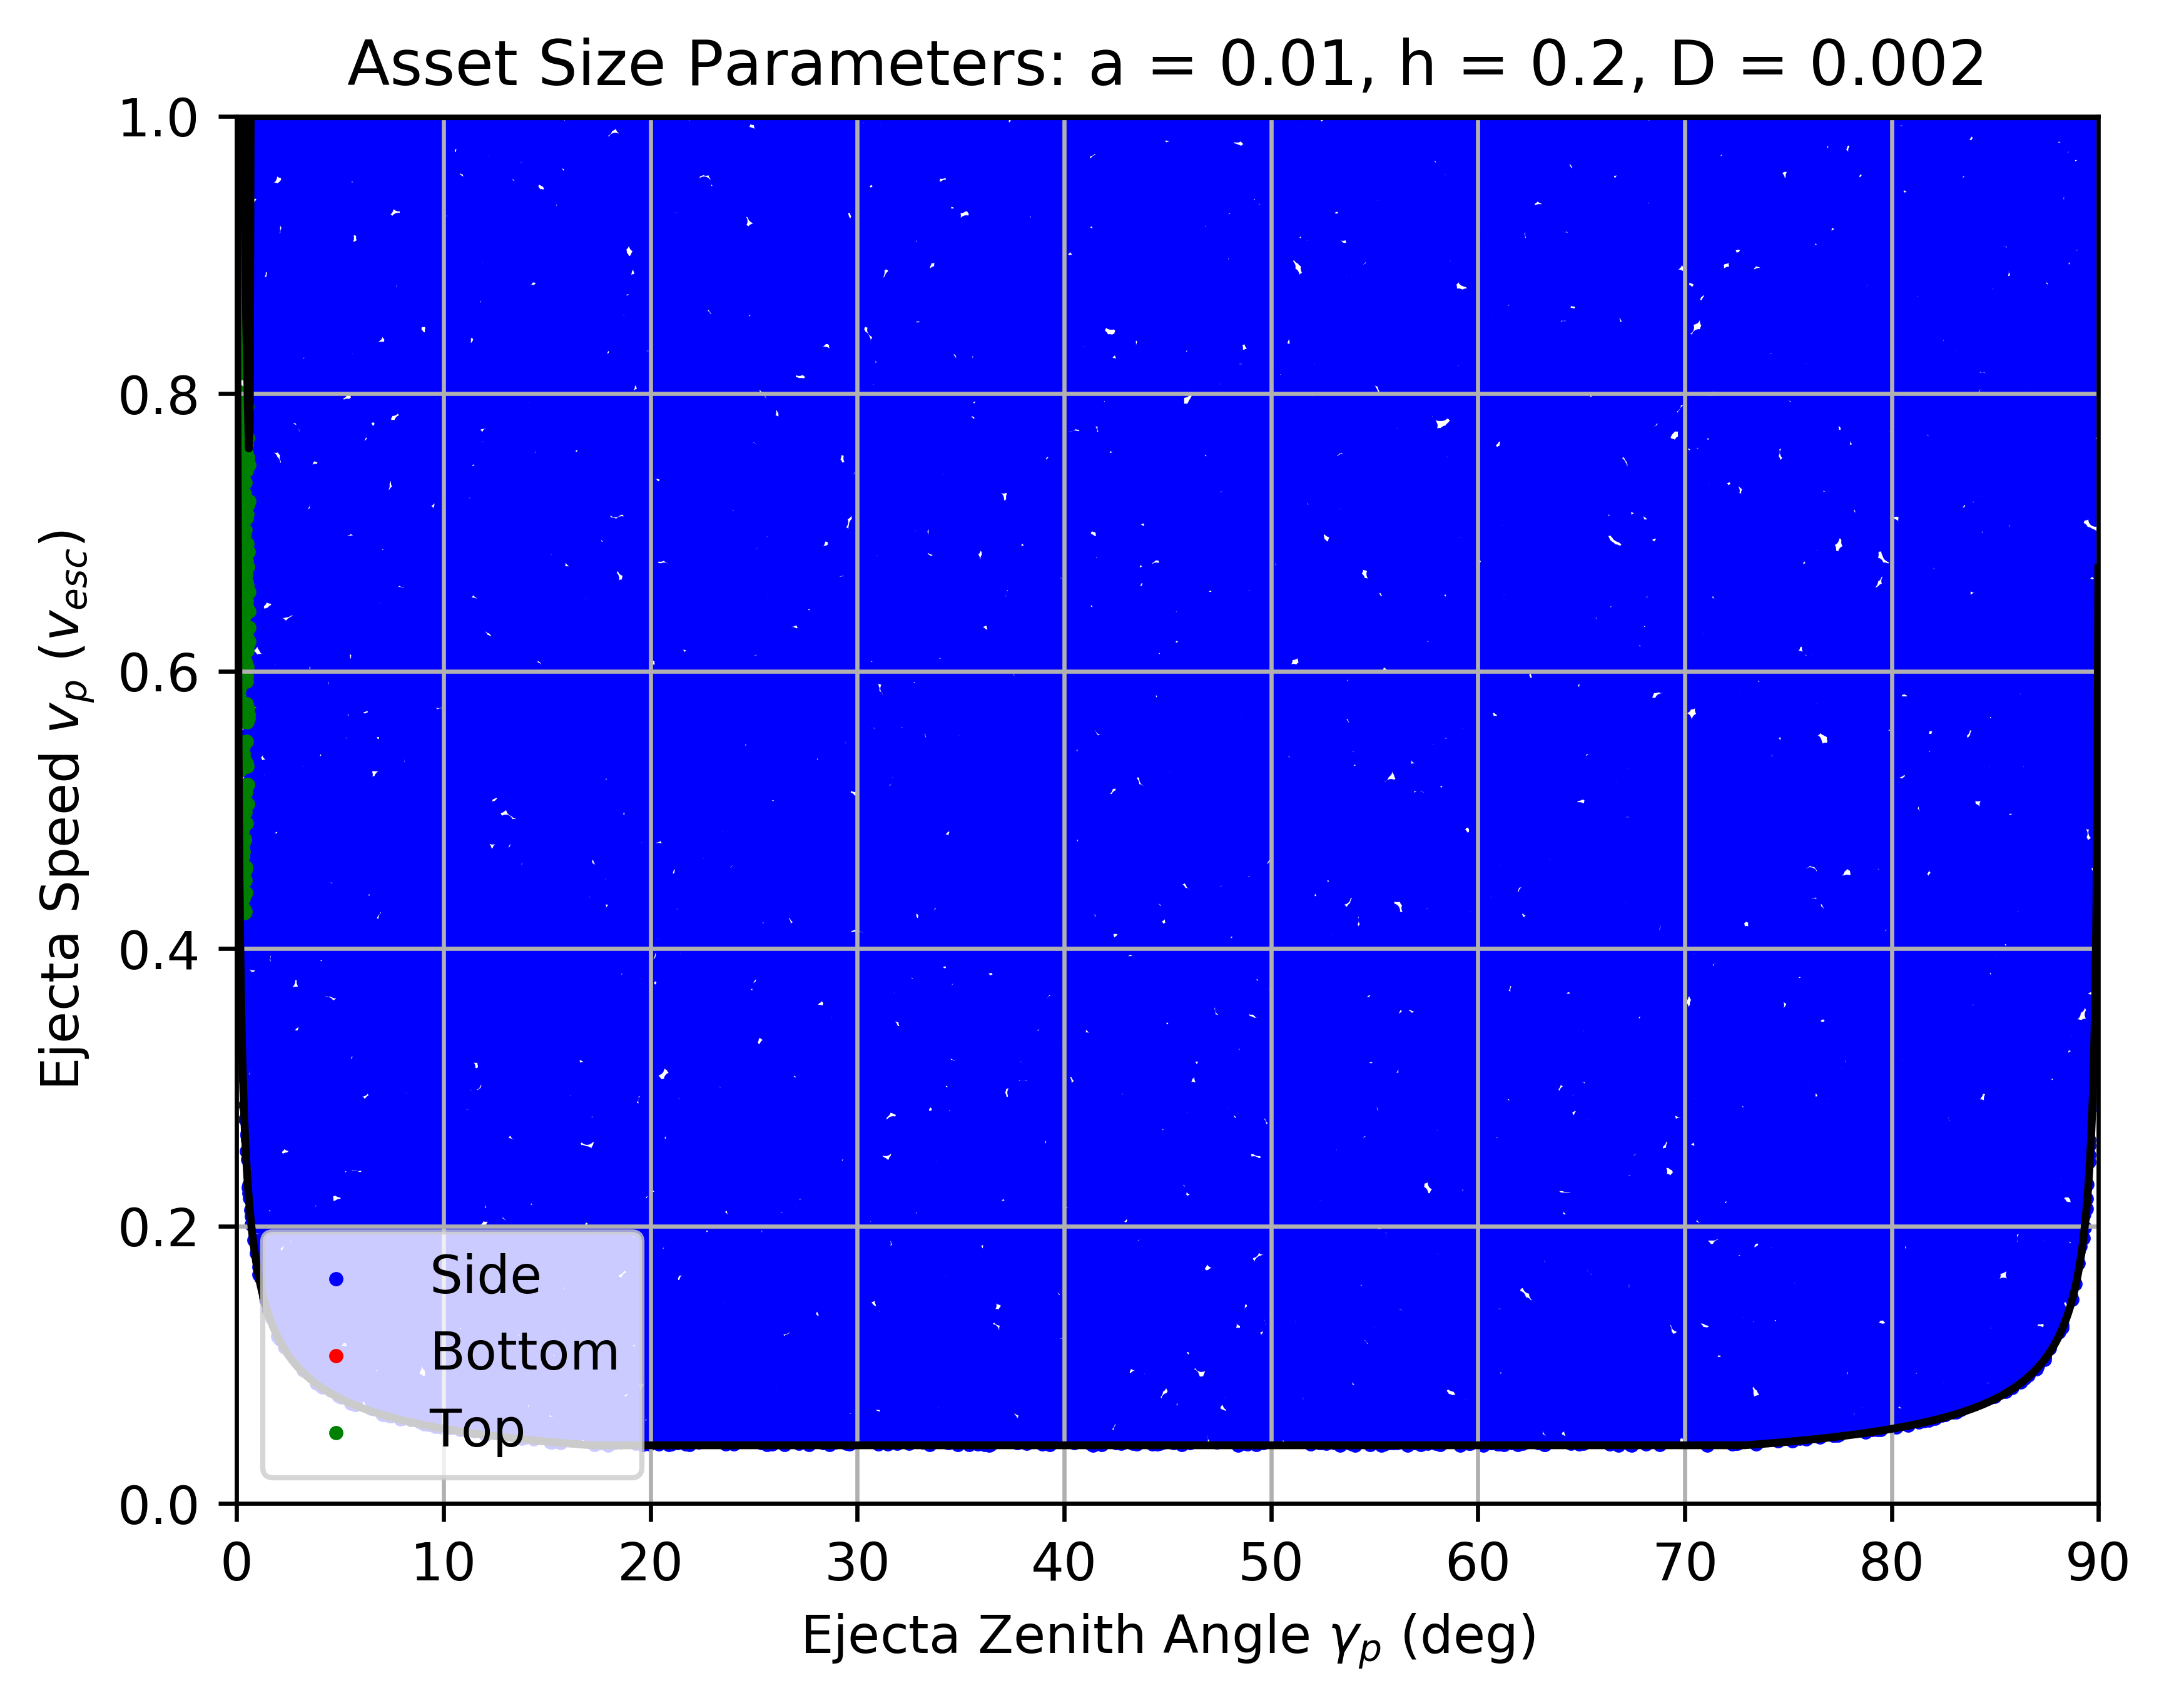
\includegraphics[width=.95\linewidth]{asset_speed_zenith_plot_1.000e-02_2.000e-01_2.000e-03.png}  
		%\caption{Put your sub-caption here}
		\label{fig:sub-asset_speed_zenith_1}
	\end{subfigure}
	\begin{subfigure}[t]{.32\textwidth}
		\centering
		% include second image
		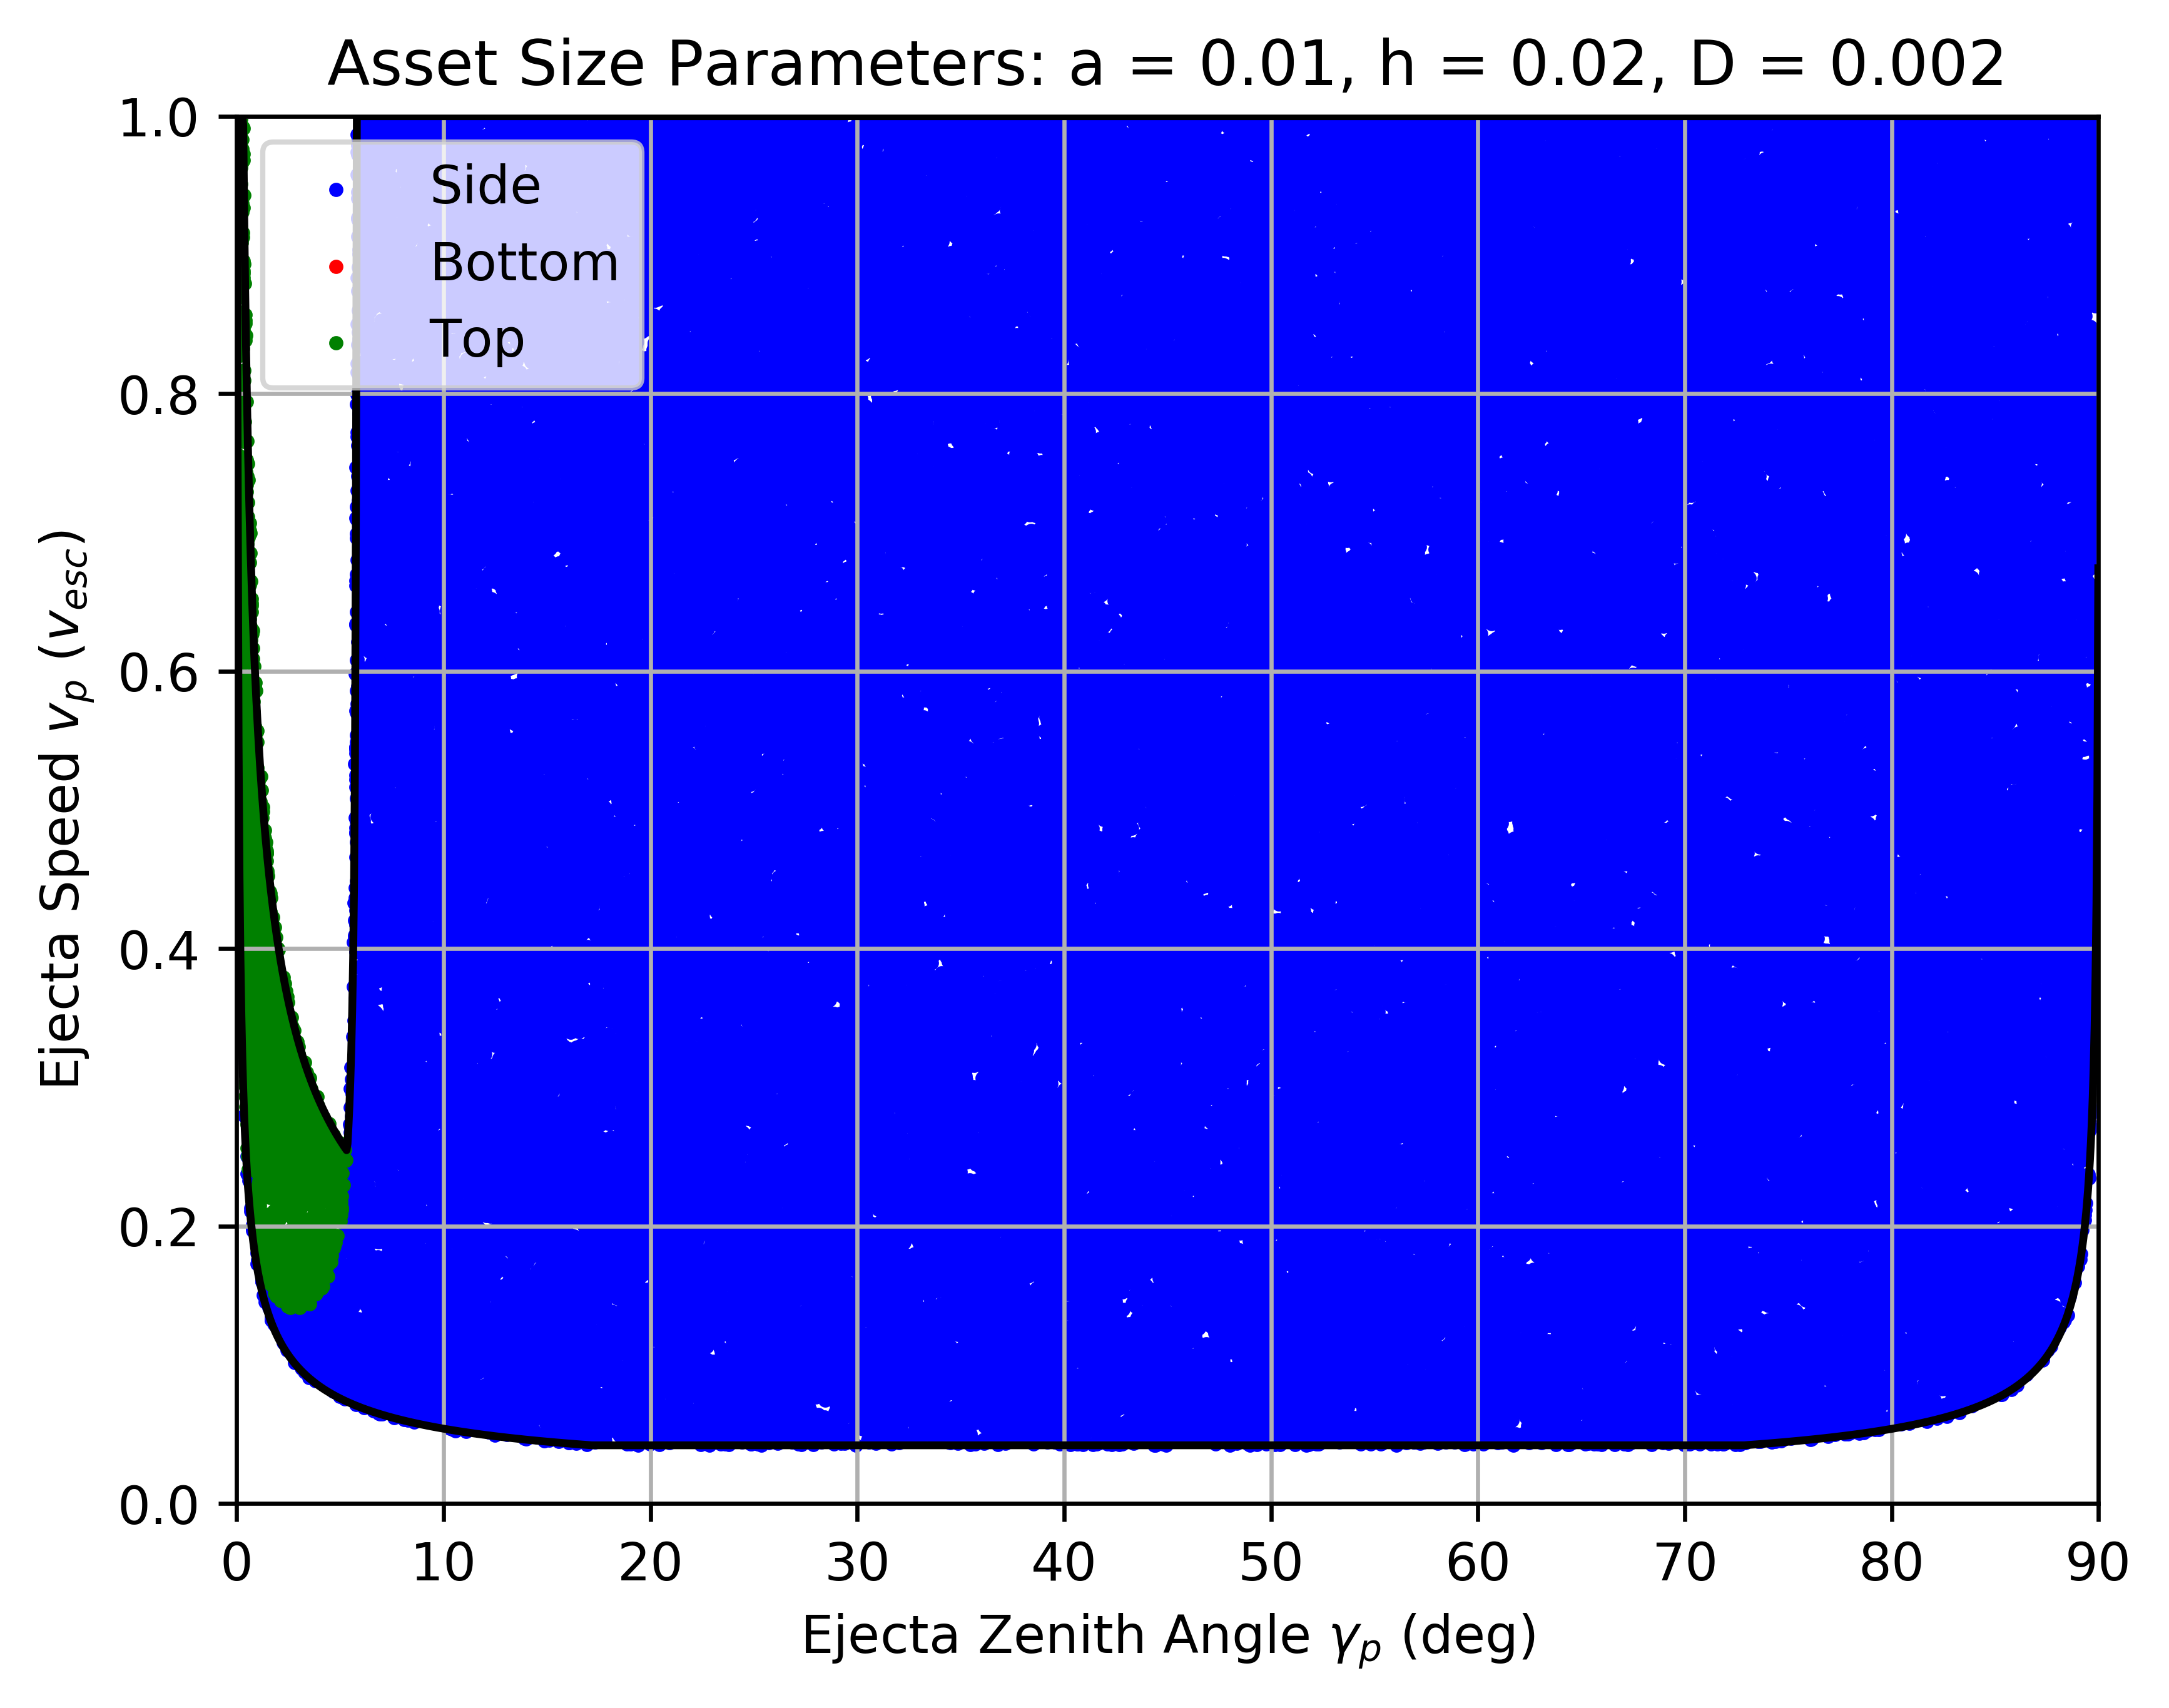
\includegraphics[width=.95\linewidth]{asset_speed_zenith_plot_1.000e-02_2.000e-02_2.000e-03.png}  
		%\caption{Put your sub-caption here}
		\label{fig:sub-asset_speed_zenith_2}
	\end{subfigure}
	\begin{subfigure}[t]{.32\textwidth}
		\centering
		% include second image
		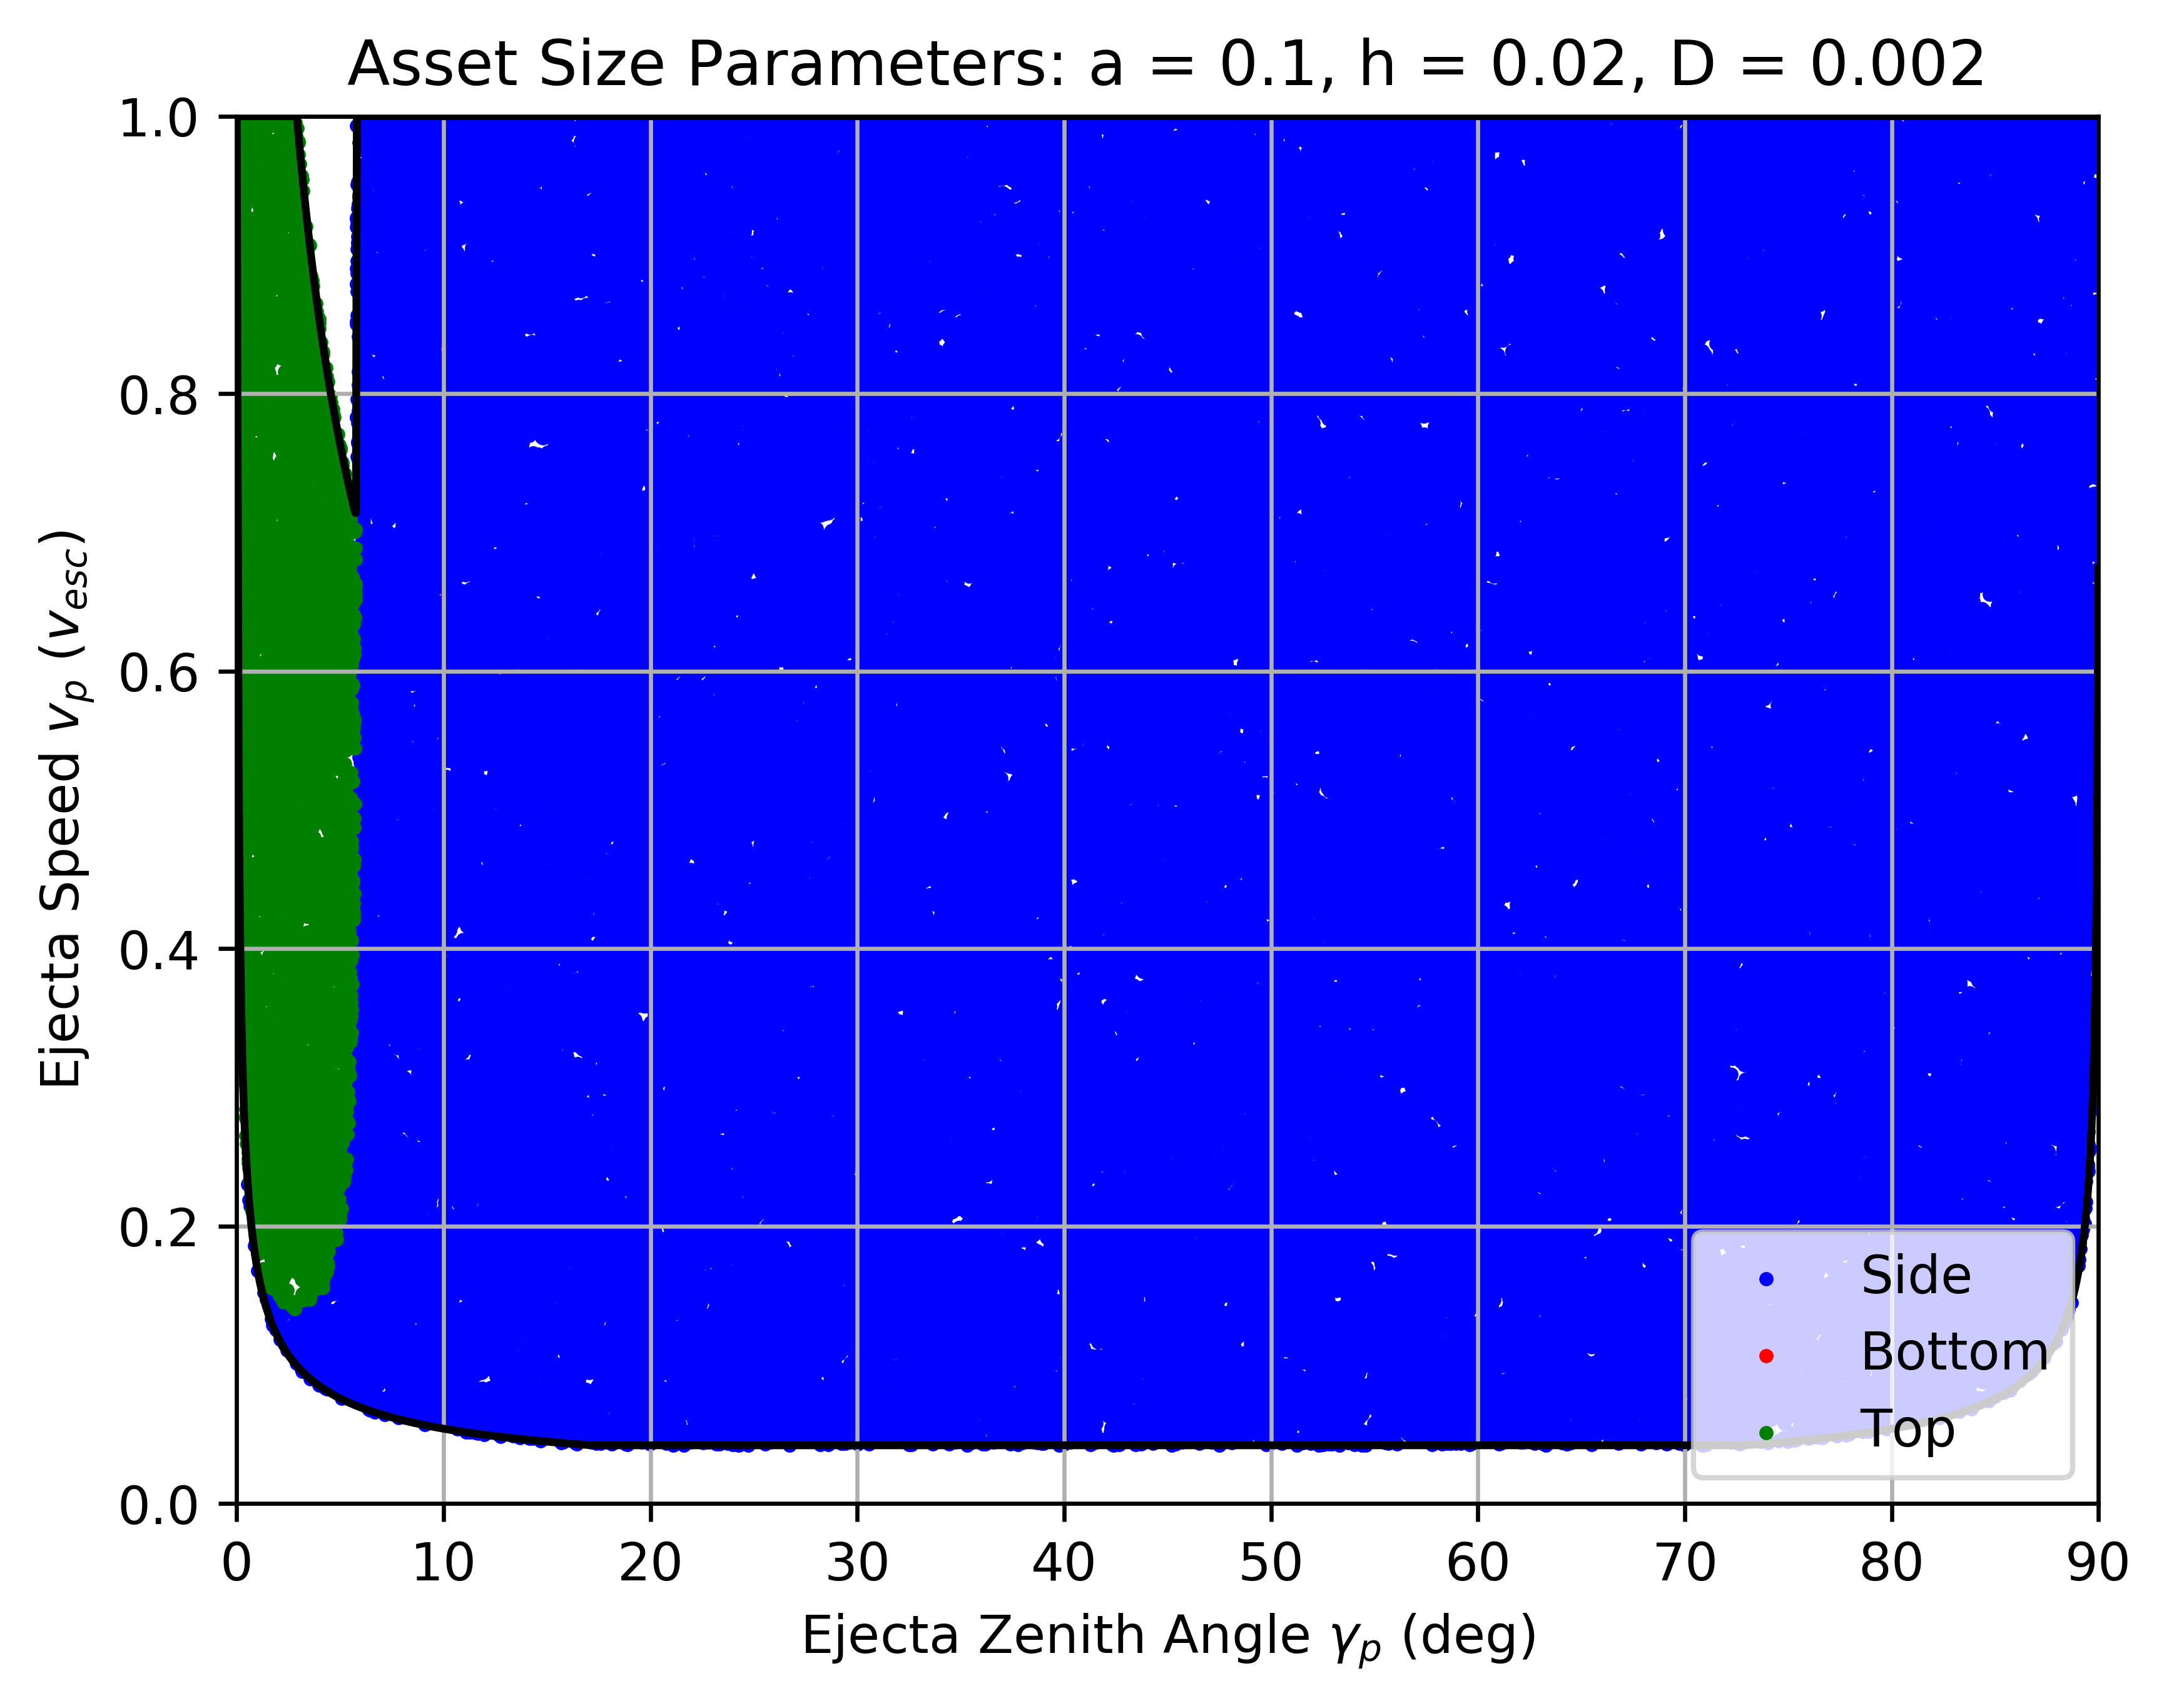
\includegraphics[width=.95\linewidth]{asset_speed_zenith_plot_1.000e-01_2.000e-02_2.000e-03.png}  
		%\caption{Put your sub-caption here}
		\label{fig:sub-asset_speed_zenith_3}
	\end{subfigure}
	
	%\newline
	
	\begin{subfigure}[t]{.32\textwidth}
		\centering
		% include third image
		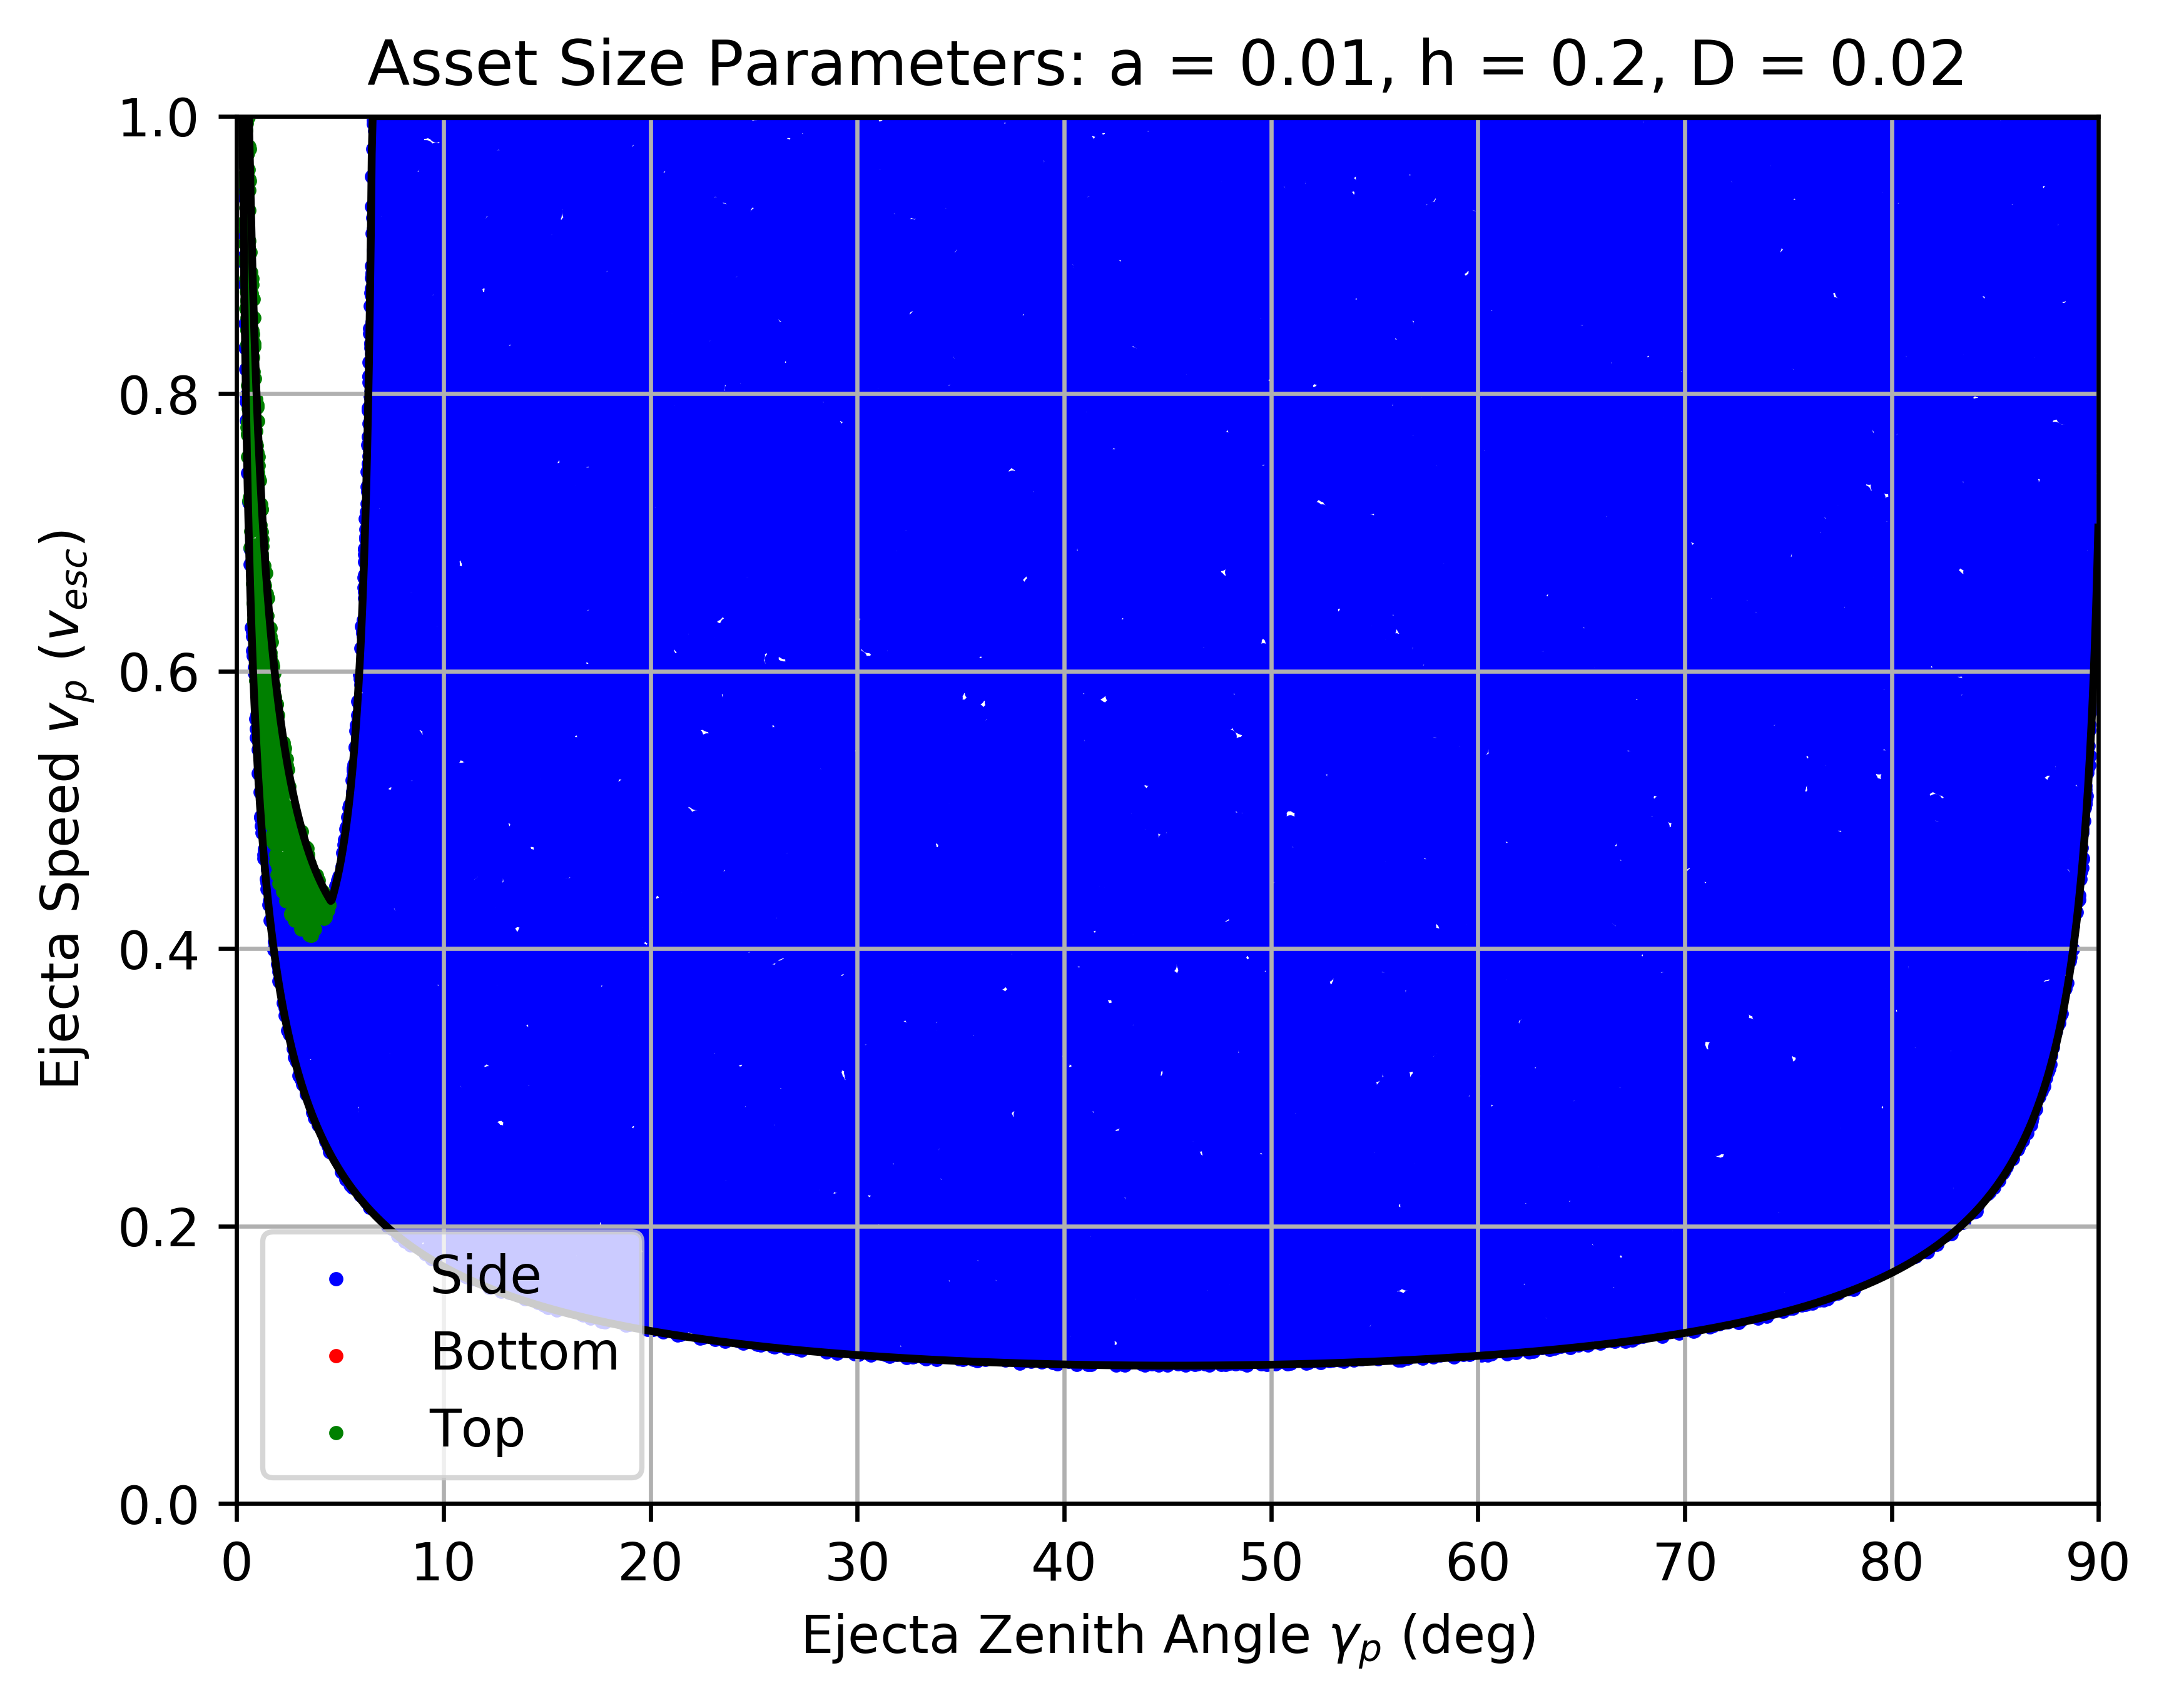
\includegraphics[width=.98\linewidth]{asset_speed_zenith_plot_1.000e-02_2.000e-01_2.000e-02.png}  
		%\caption{Put your sub-caption here}
		\label{fig:sub-asset_speed_zenith_4}
	\end{subfigure}
	\begin{subfigure}[t]{.32\textwidth}
		\centering
		% include fourth image
		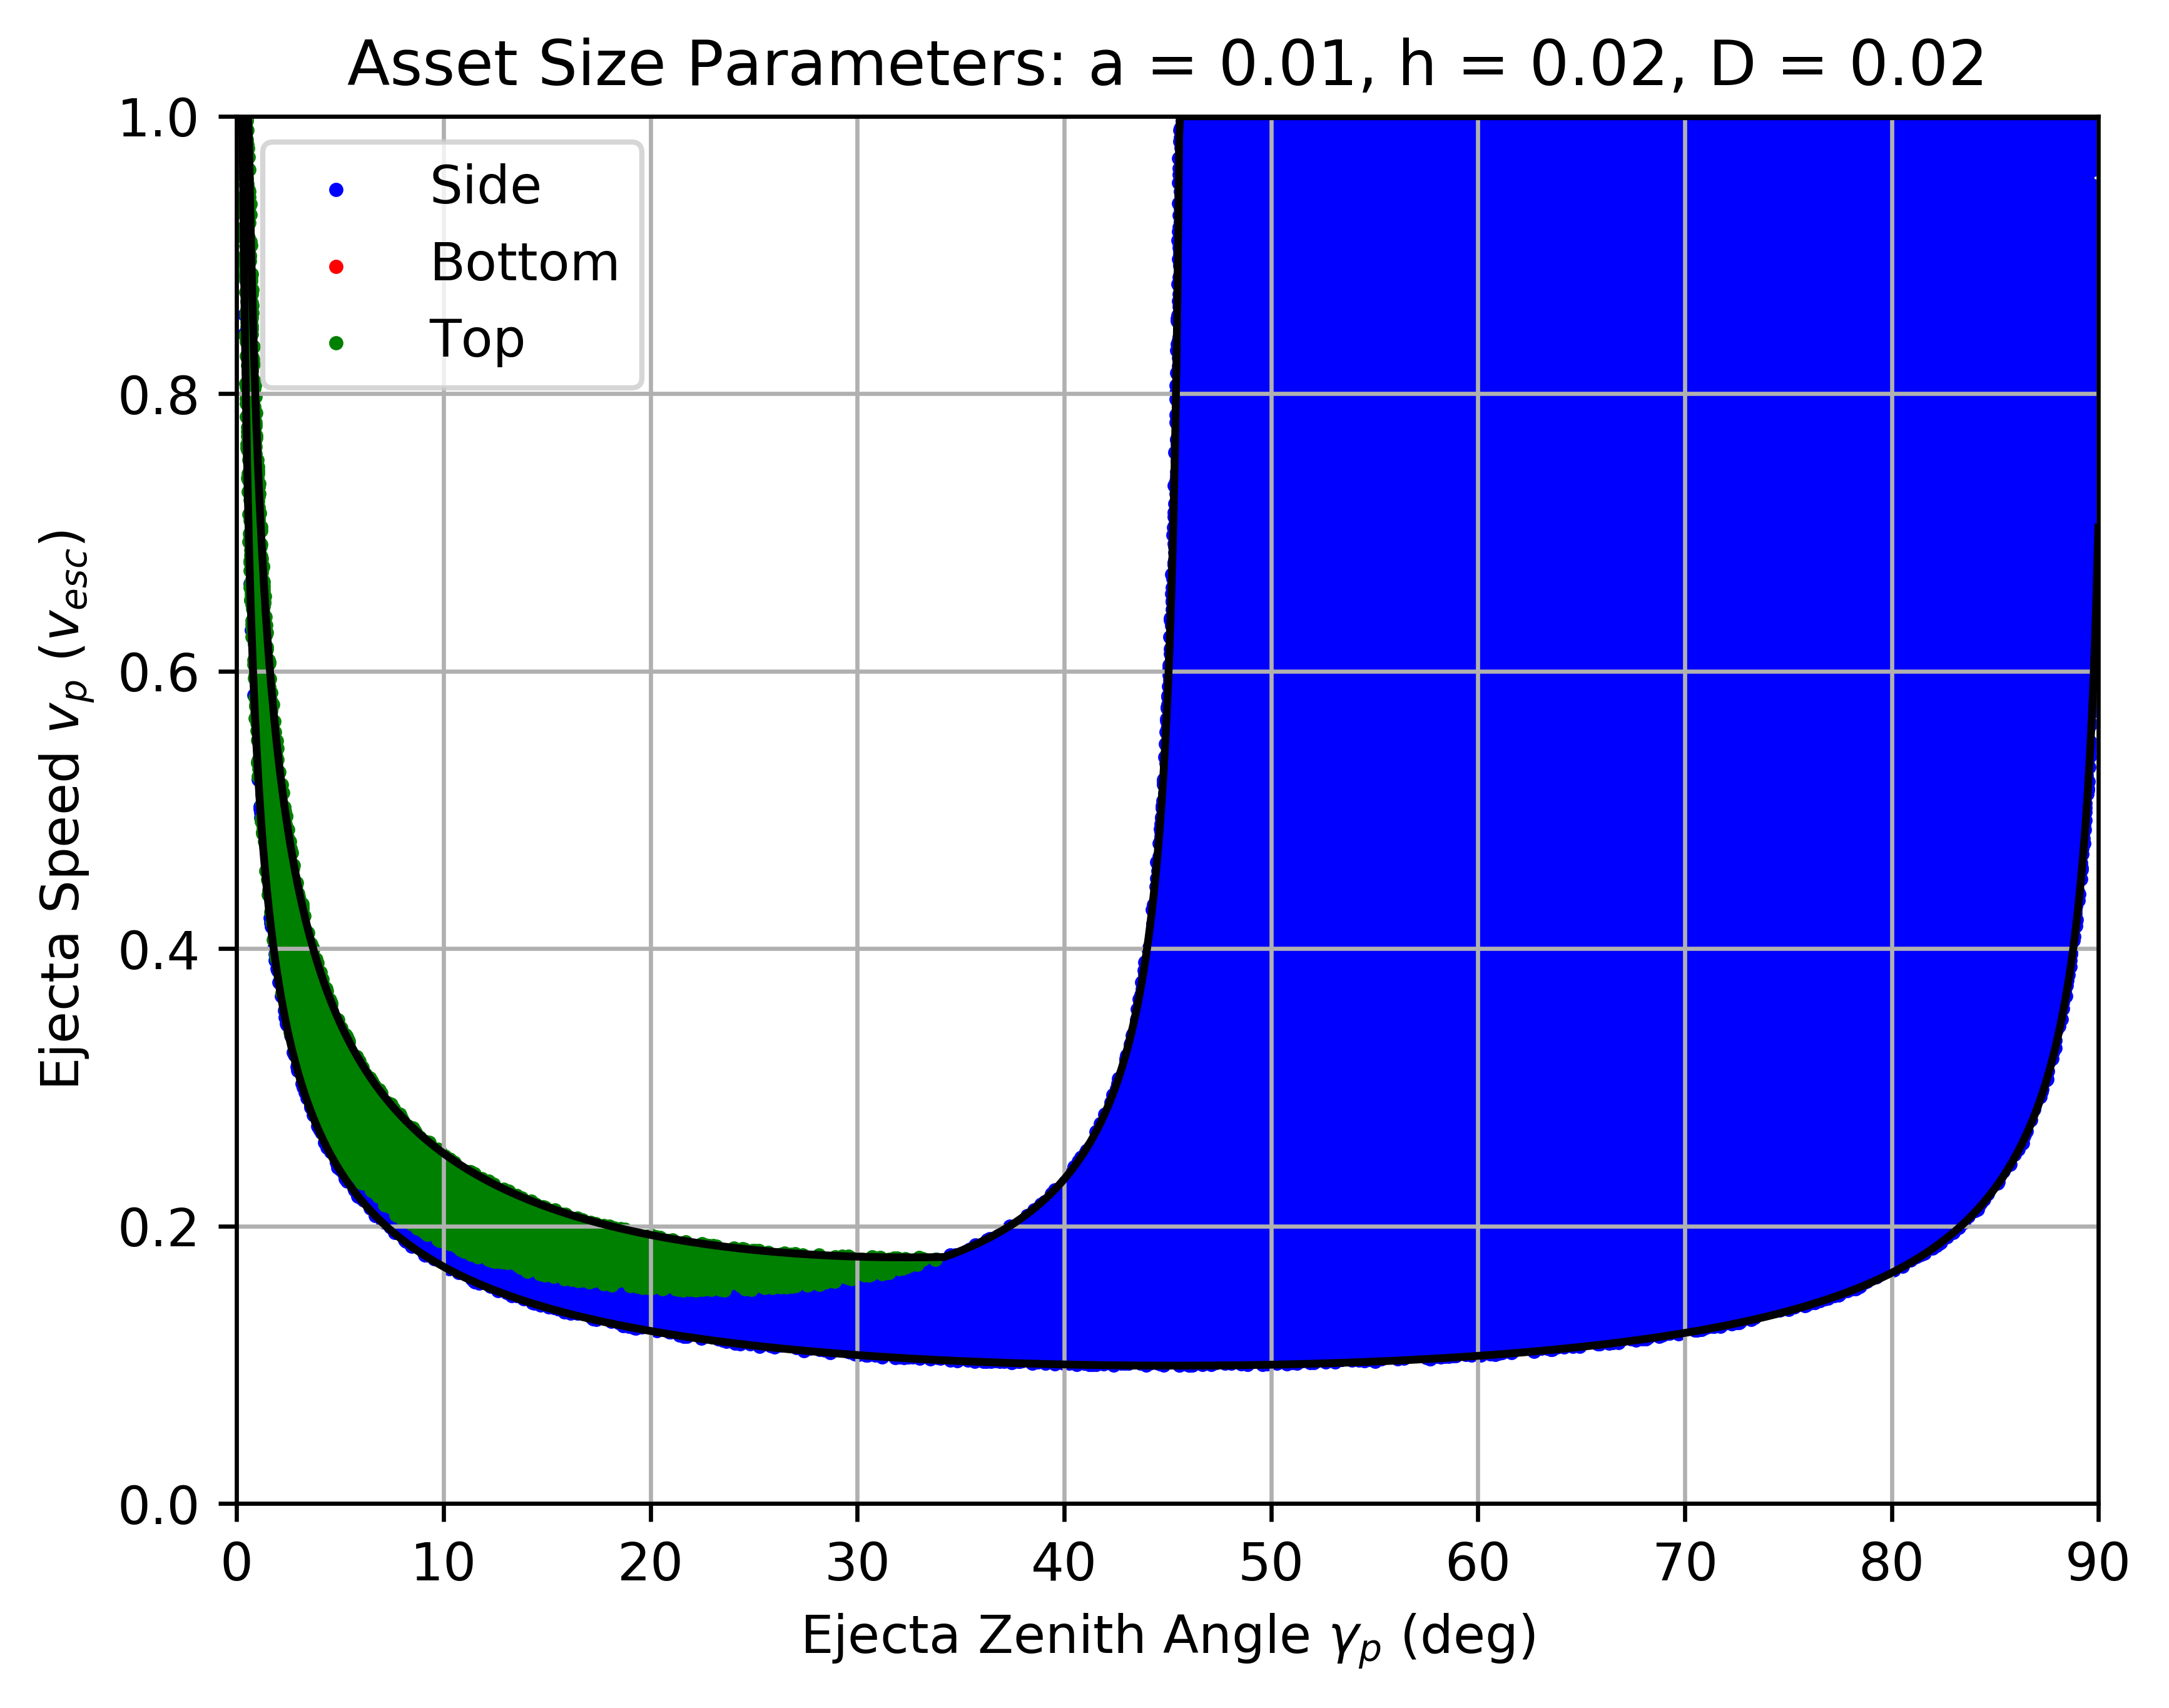
\includegraphics[width=.98\linewidth]{asset_speed_zenith_plot_1.000e-02_2.000e-02_2.000e-02.png}  
		%\caption{Put your sub-caption here}
		\label{fig:sub-asset_speed_zenith_5}
	\end{subfigure}
	\begin{subfigure}[t]{.32\textwidth}
		\centering
		% include fourth image
		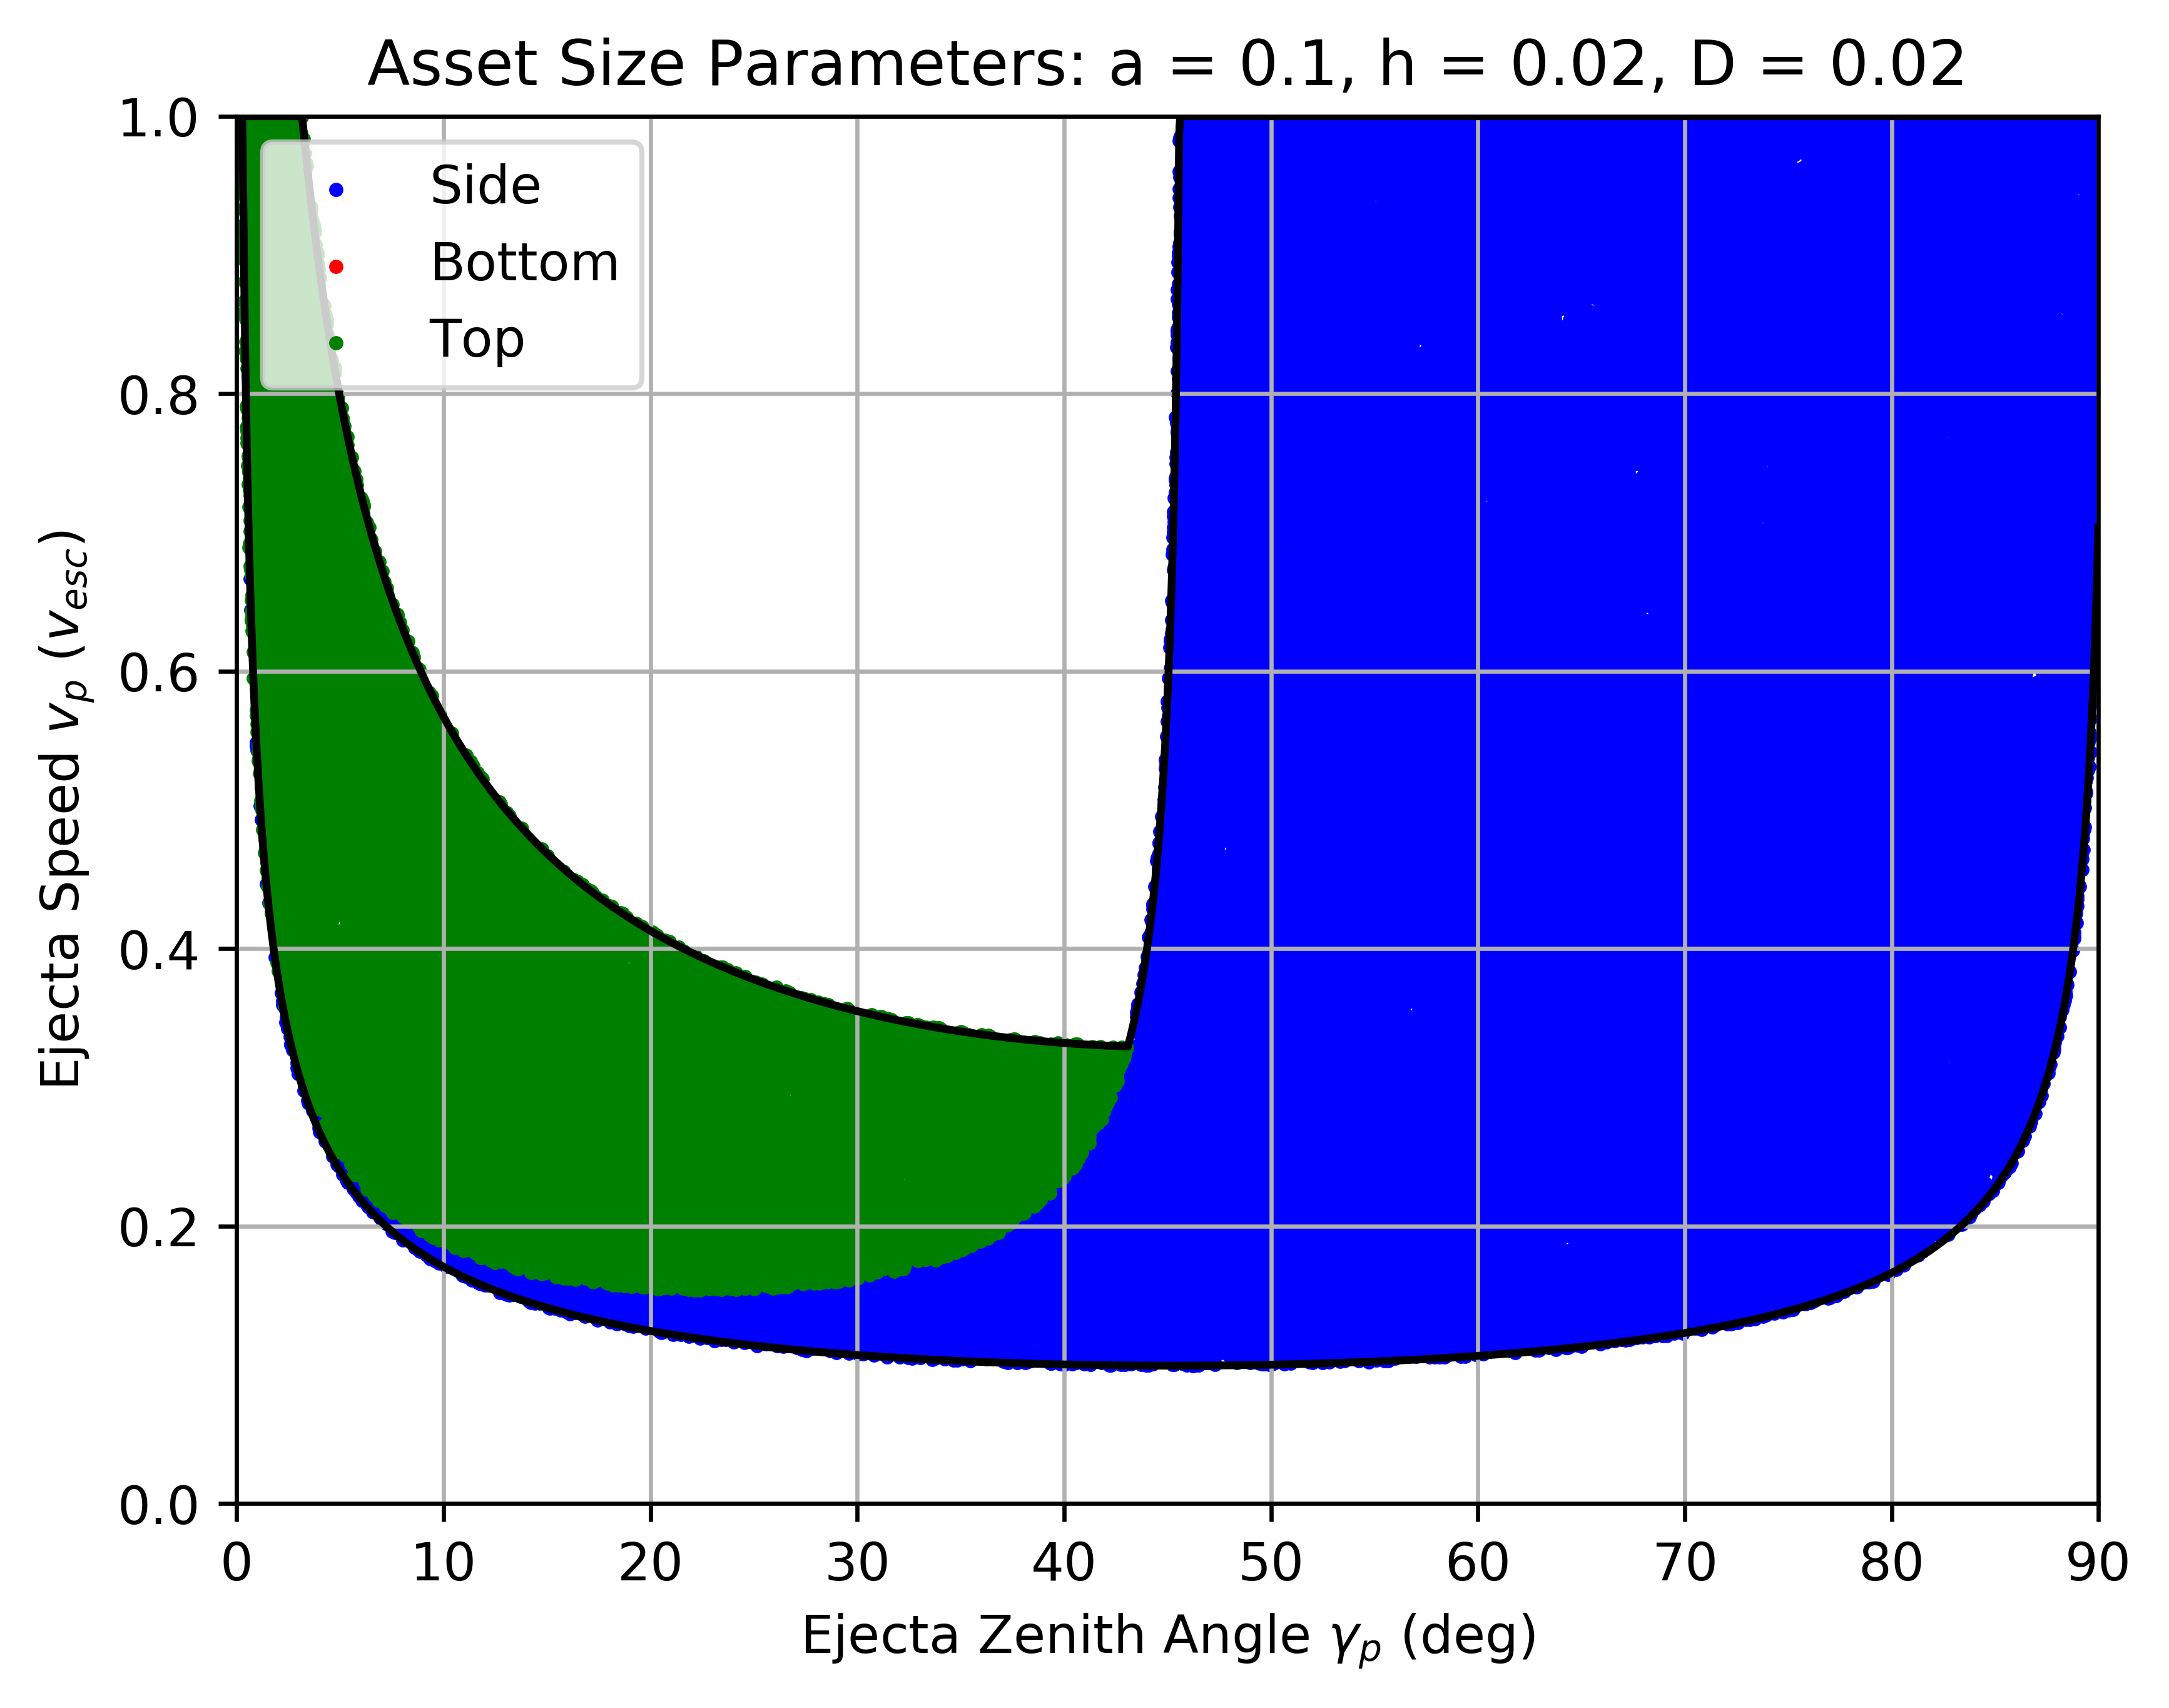
\includegraphics[width=.98\linewidth]{asset_speed_zenith_plot_1.000e-01_2.000e-02_2.000e-02.png}  
		%\caption{Put your sub-caption here}
		\label{fig:sub-asset_speed_zenith_6}
	\end{subfigure}
	
	
	\begin{subfigure}[t]{.32\textwidth}
		\centering
		% include third image
		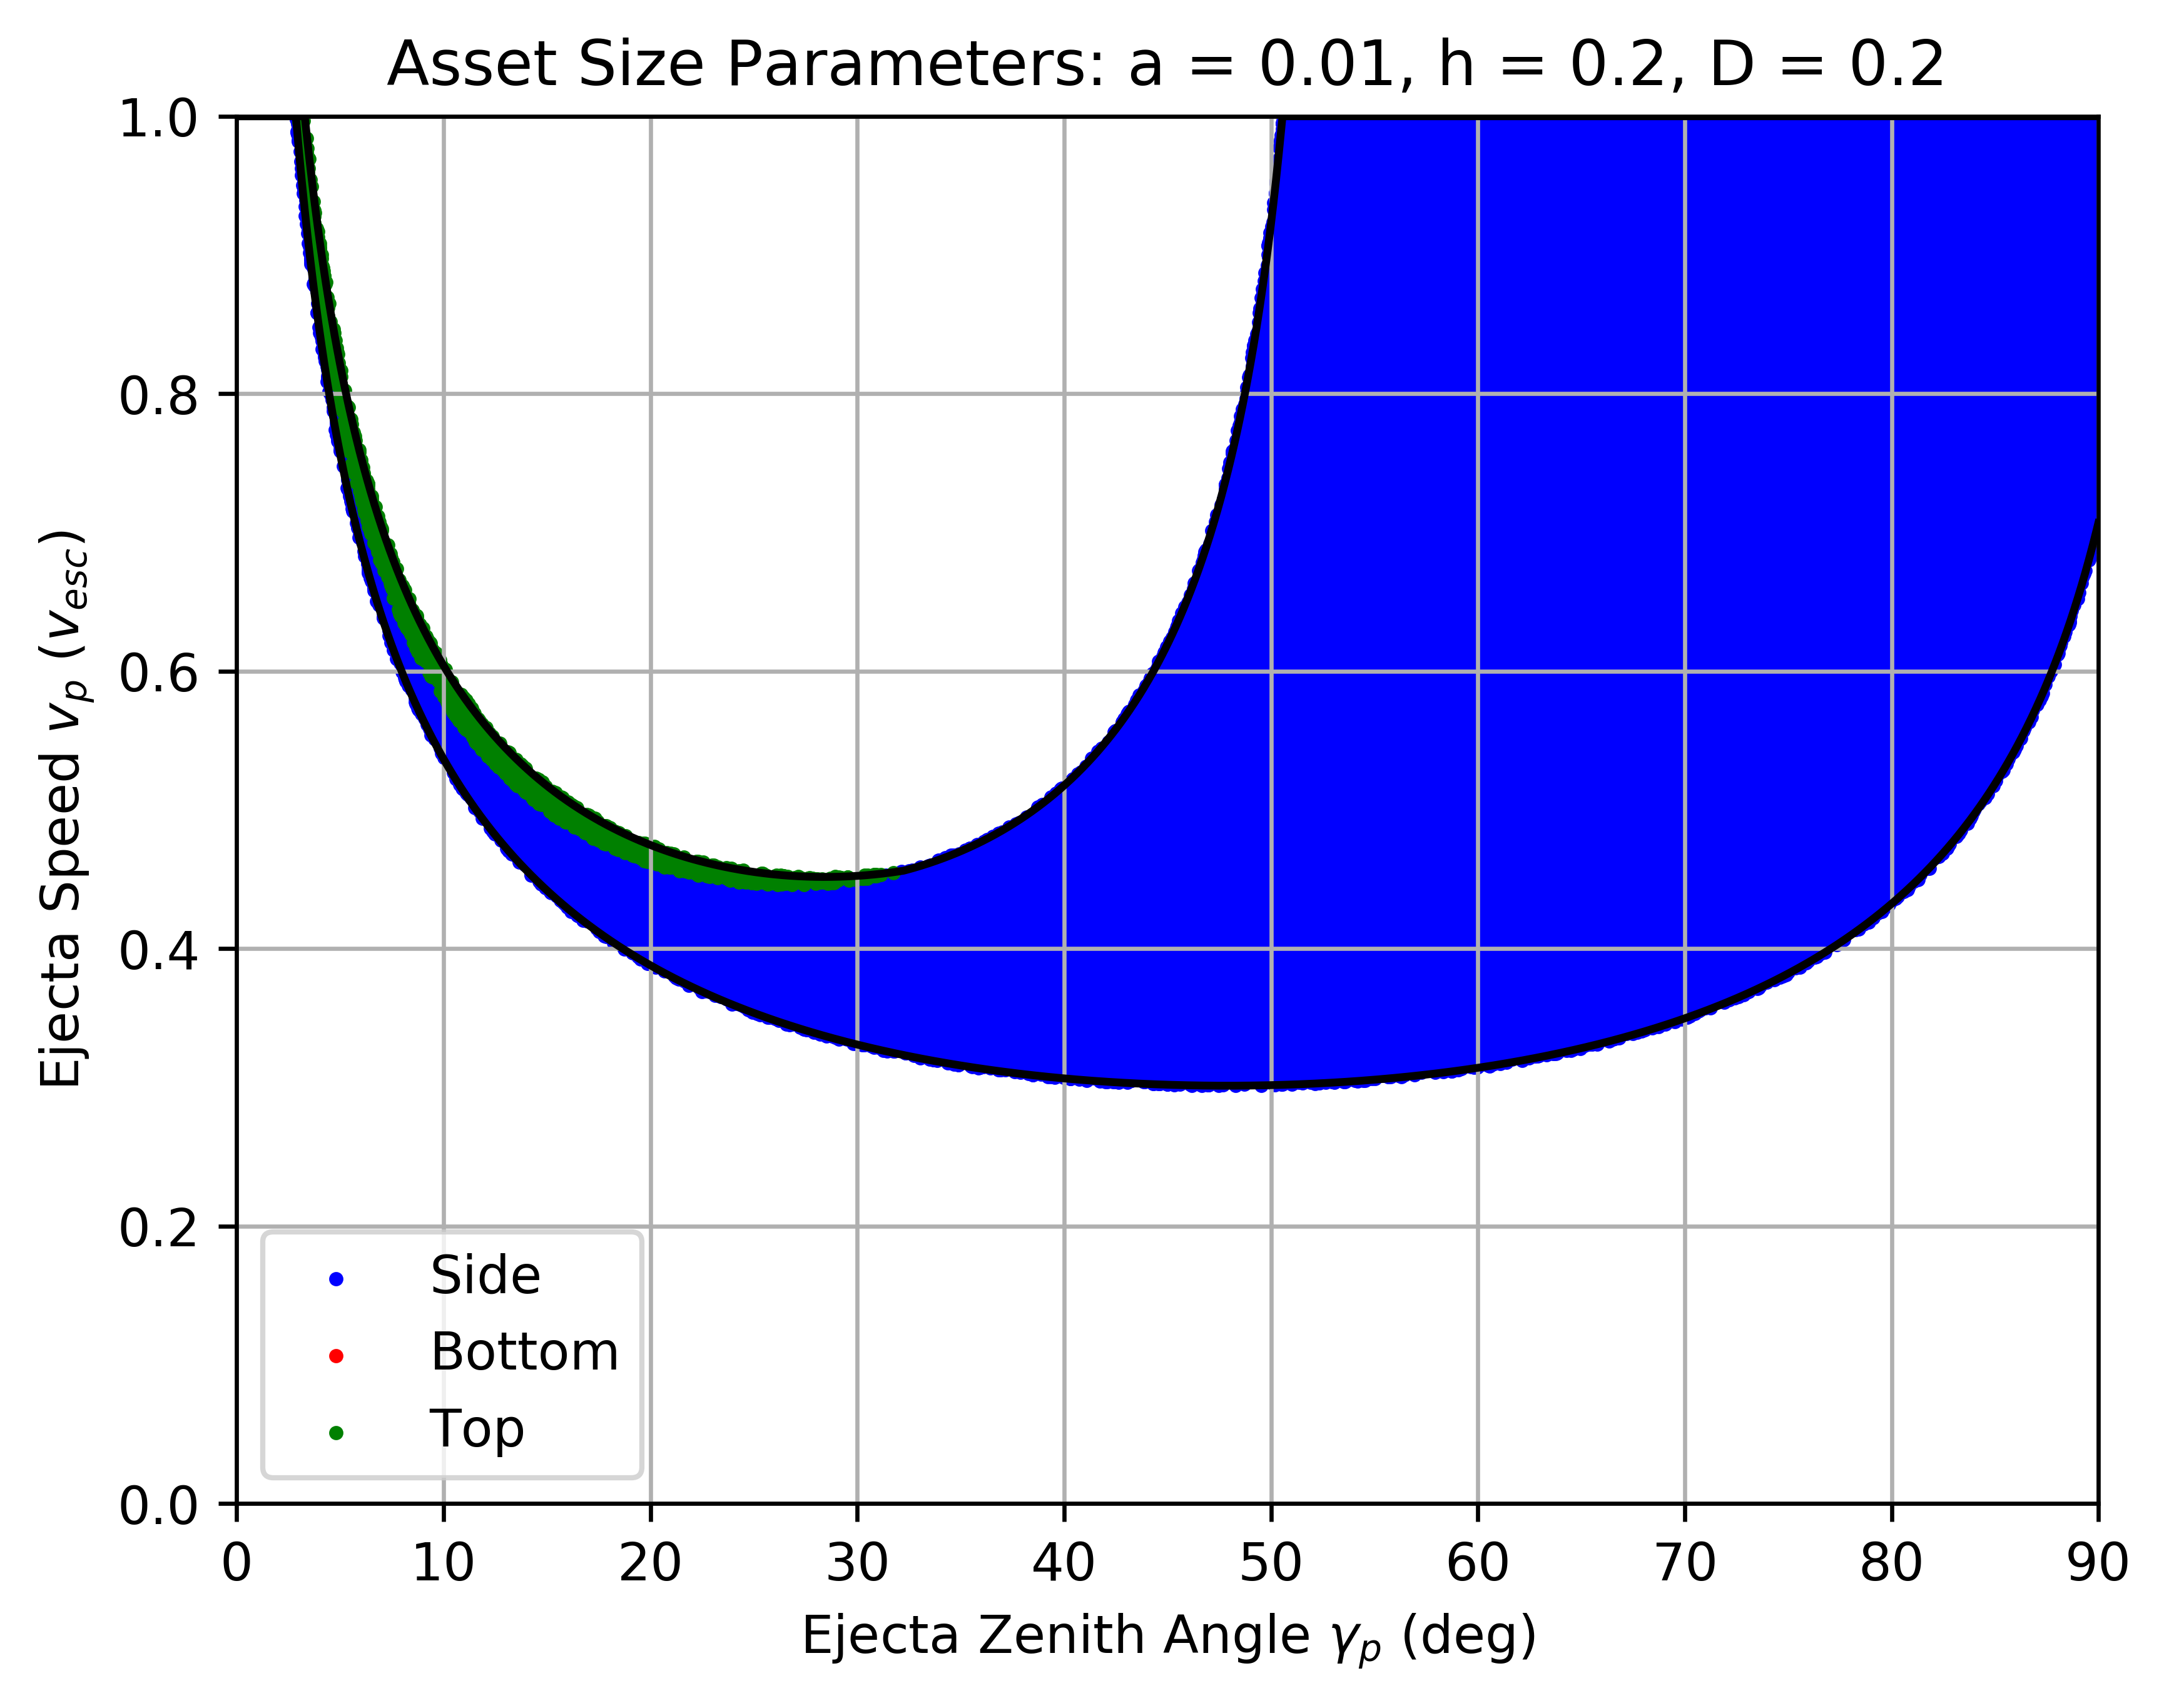
\includegraphics[width=.98\linewidth]{asset_speed_zenith_plot_1.000e-02_2.000e-01_2.000e-01.png}  
		%\caption{Put your sub-caption here}
		\label{fig:sub-asset_speed_zenith_7}
	\end{subfigure}
	\begin{subfigure}[t]{.32\textwidth}
		\centering
		% include fourth image
		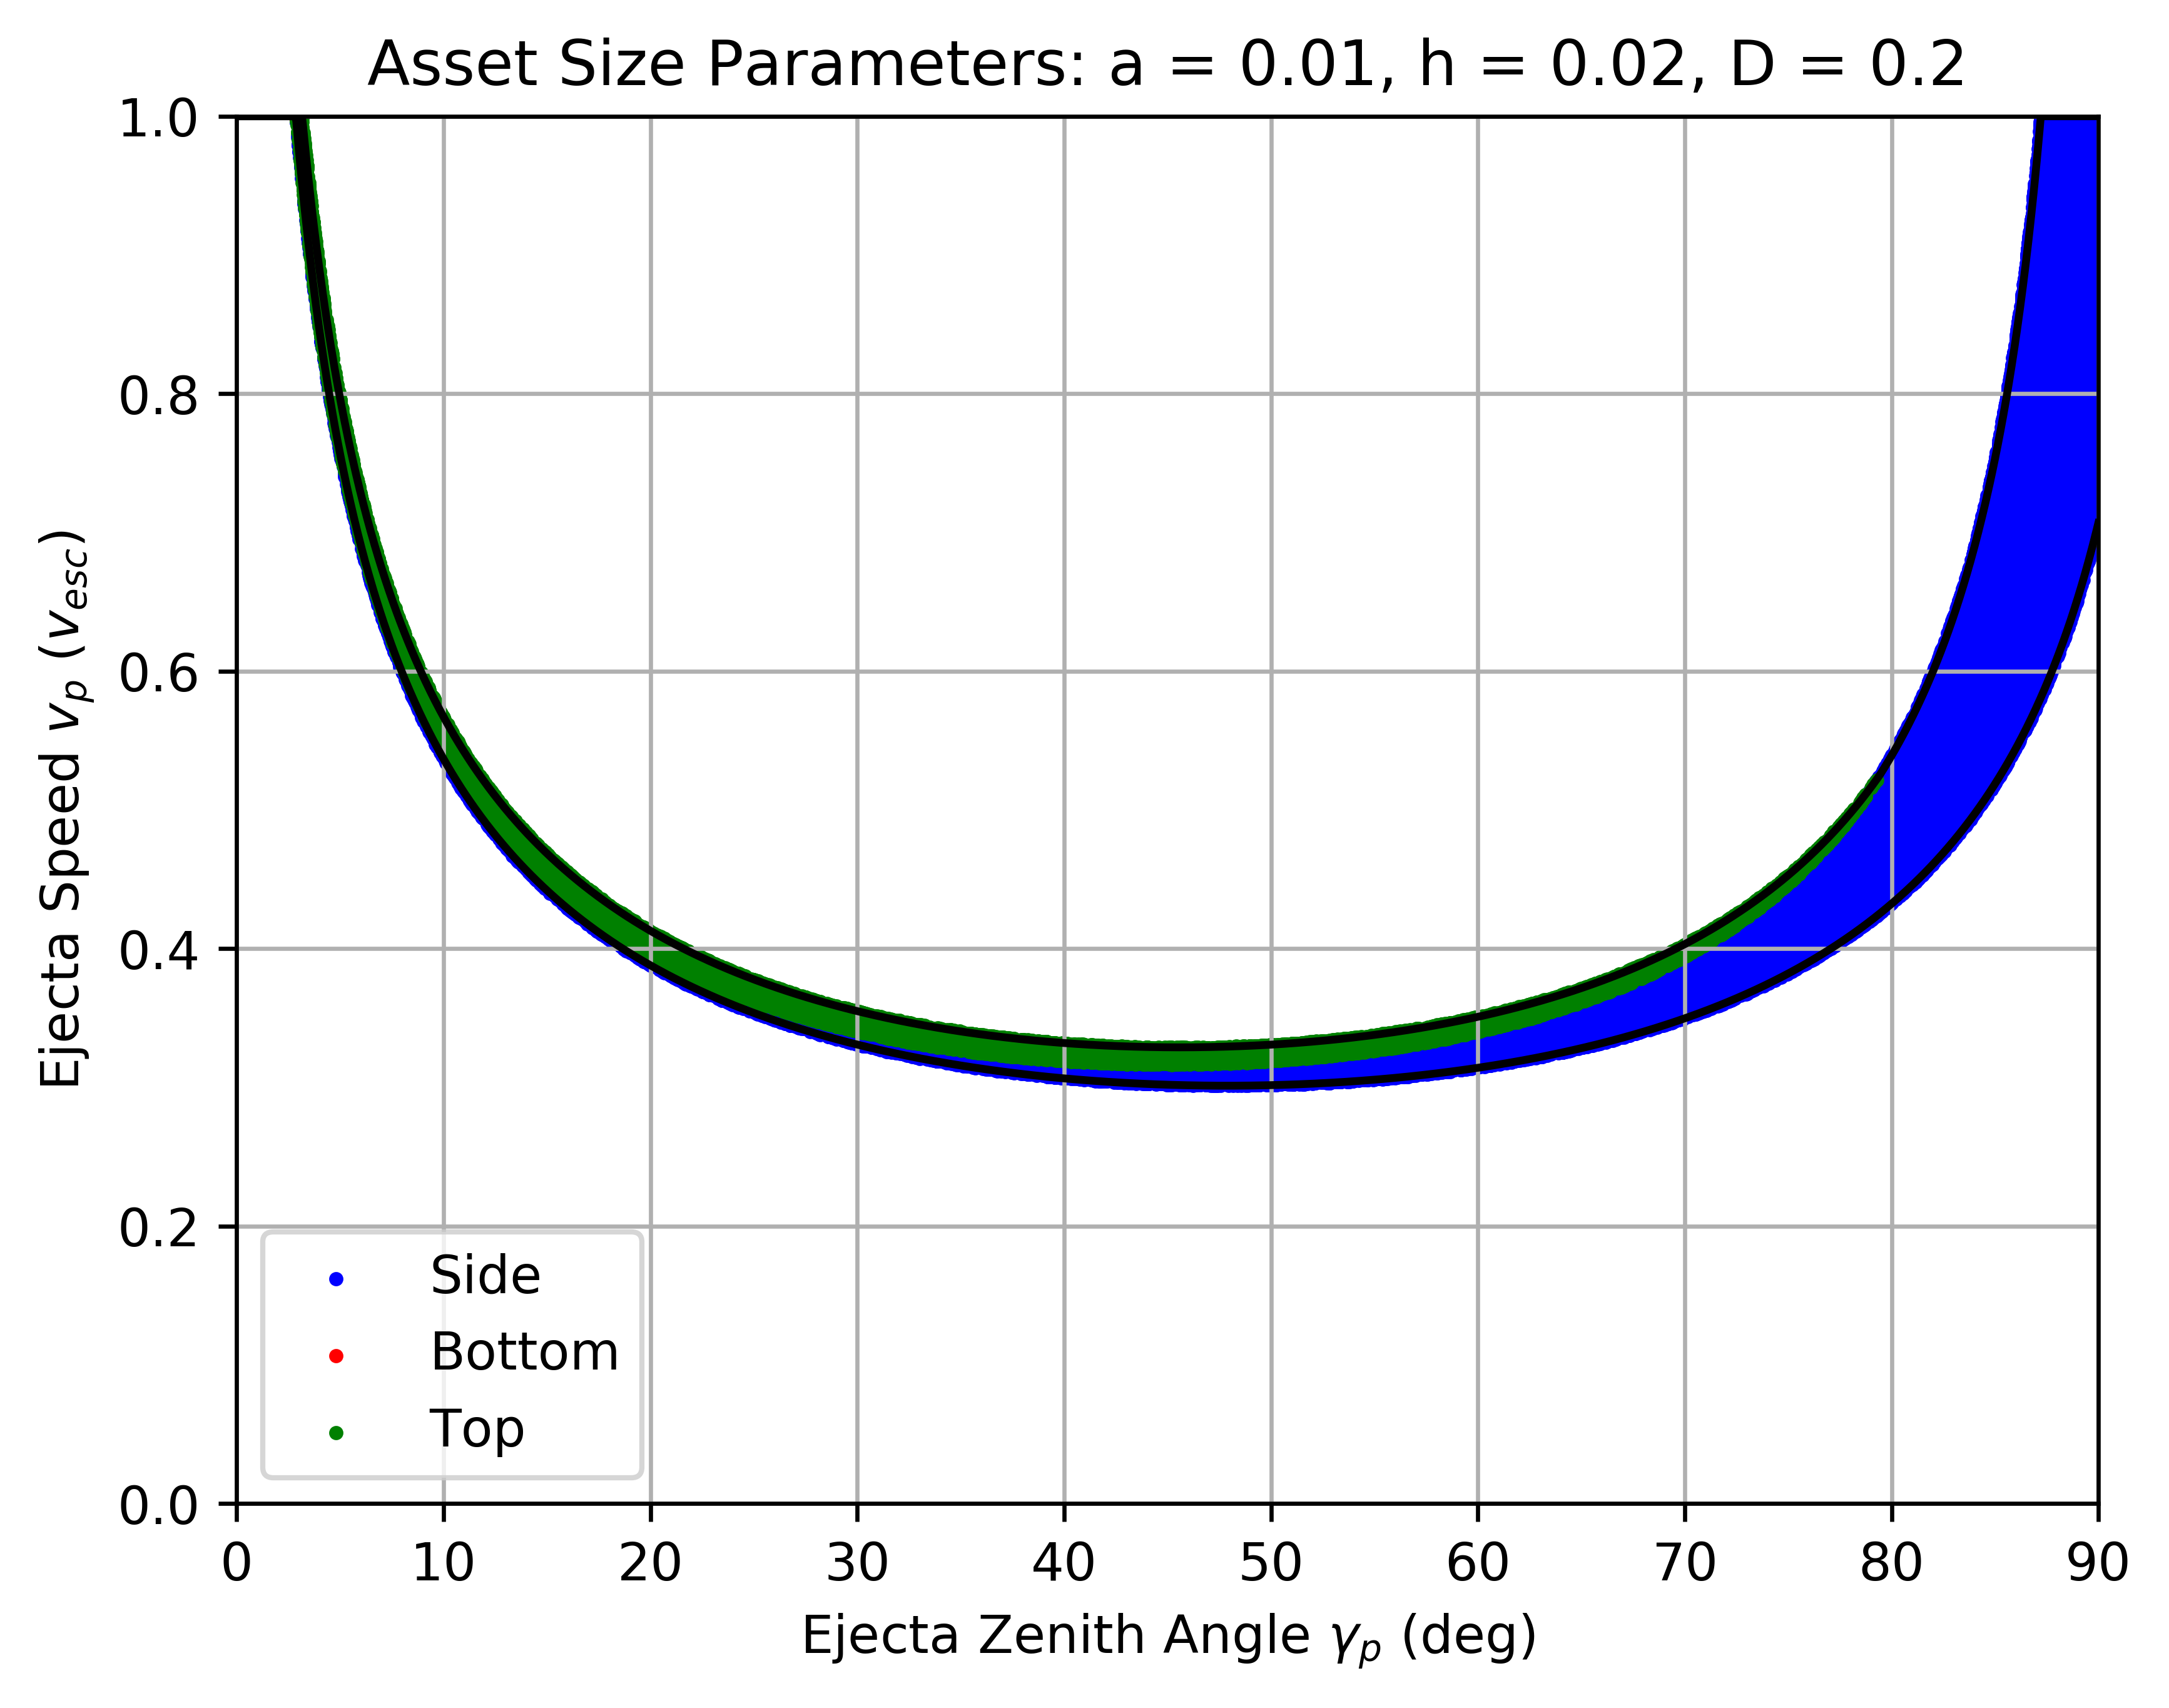
\includegraphics[width=.98\linewidth]{asset_speed_zenith_plot_1.000e-02_2.000e-02_2.000e-01.png}  
		%\caption{Put your sub-caption here}
		\label{fig:sub-asset_speed_zenith_8}
	\end{subfigure}
	\begin{subfigure}[t]{.32\textwidth}
		\centering
		% include fourth image
		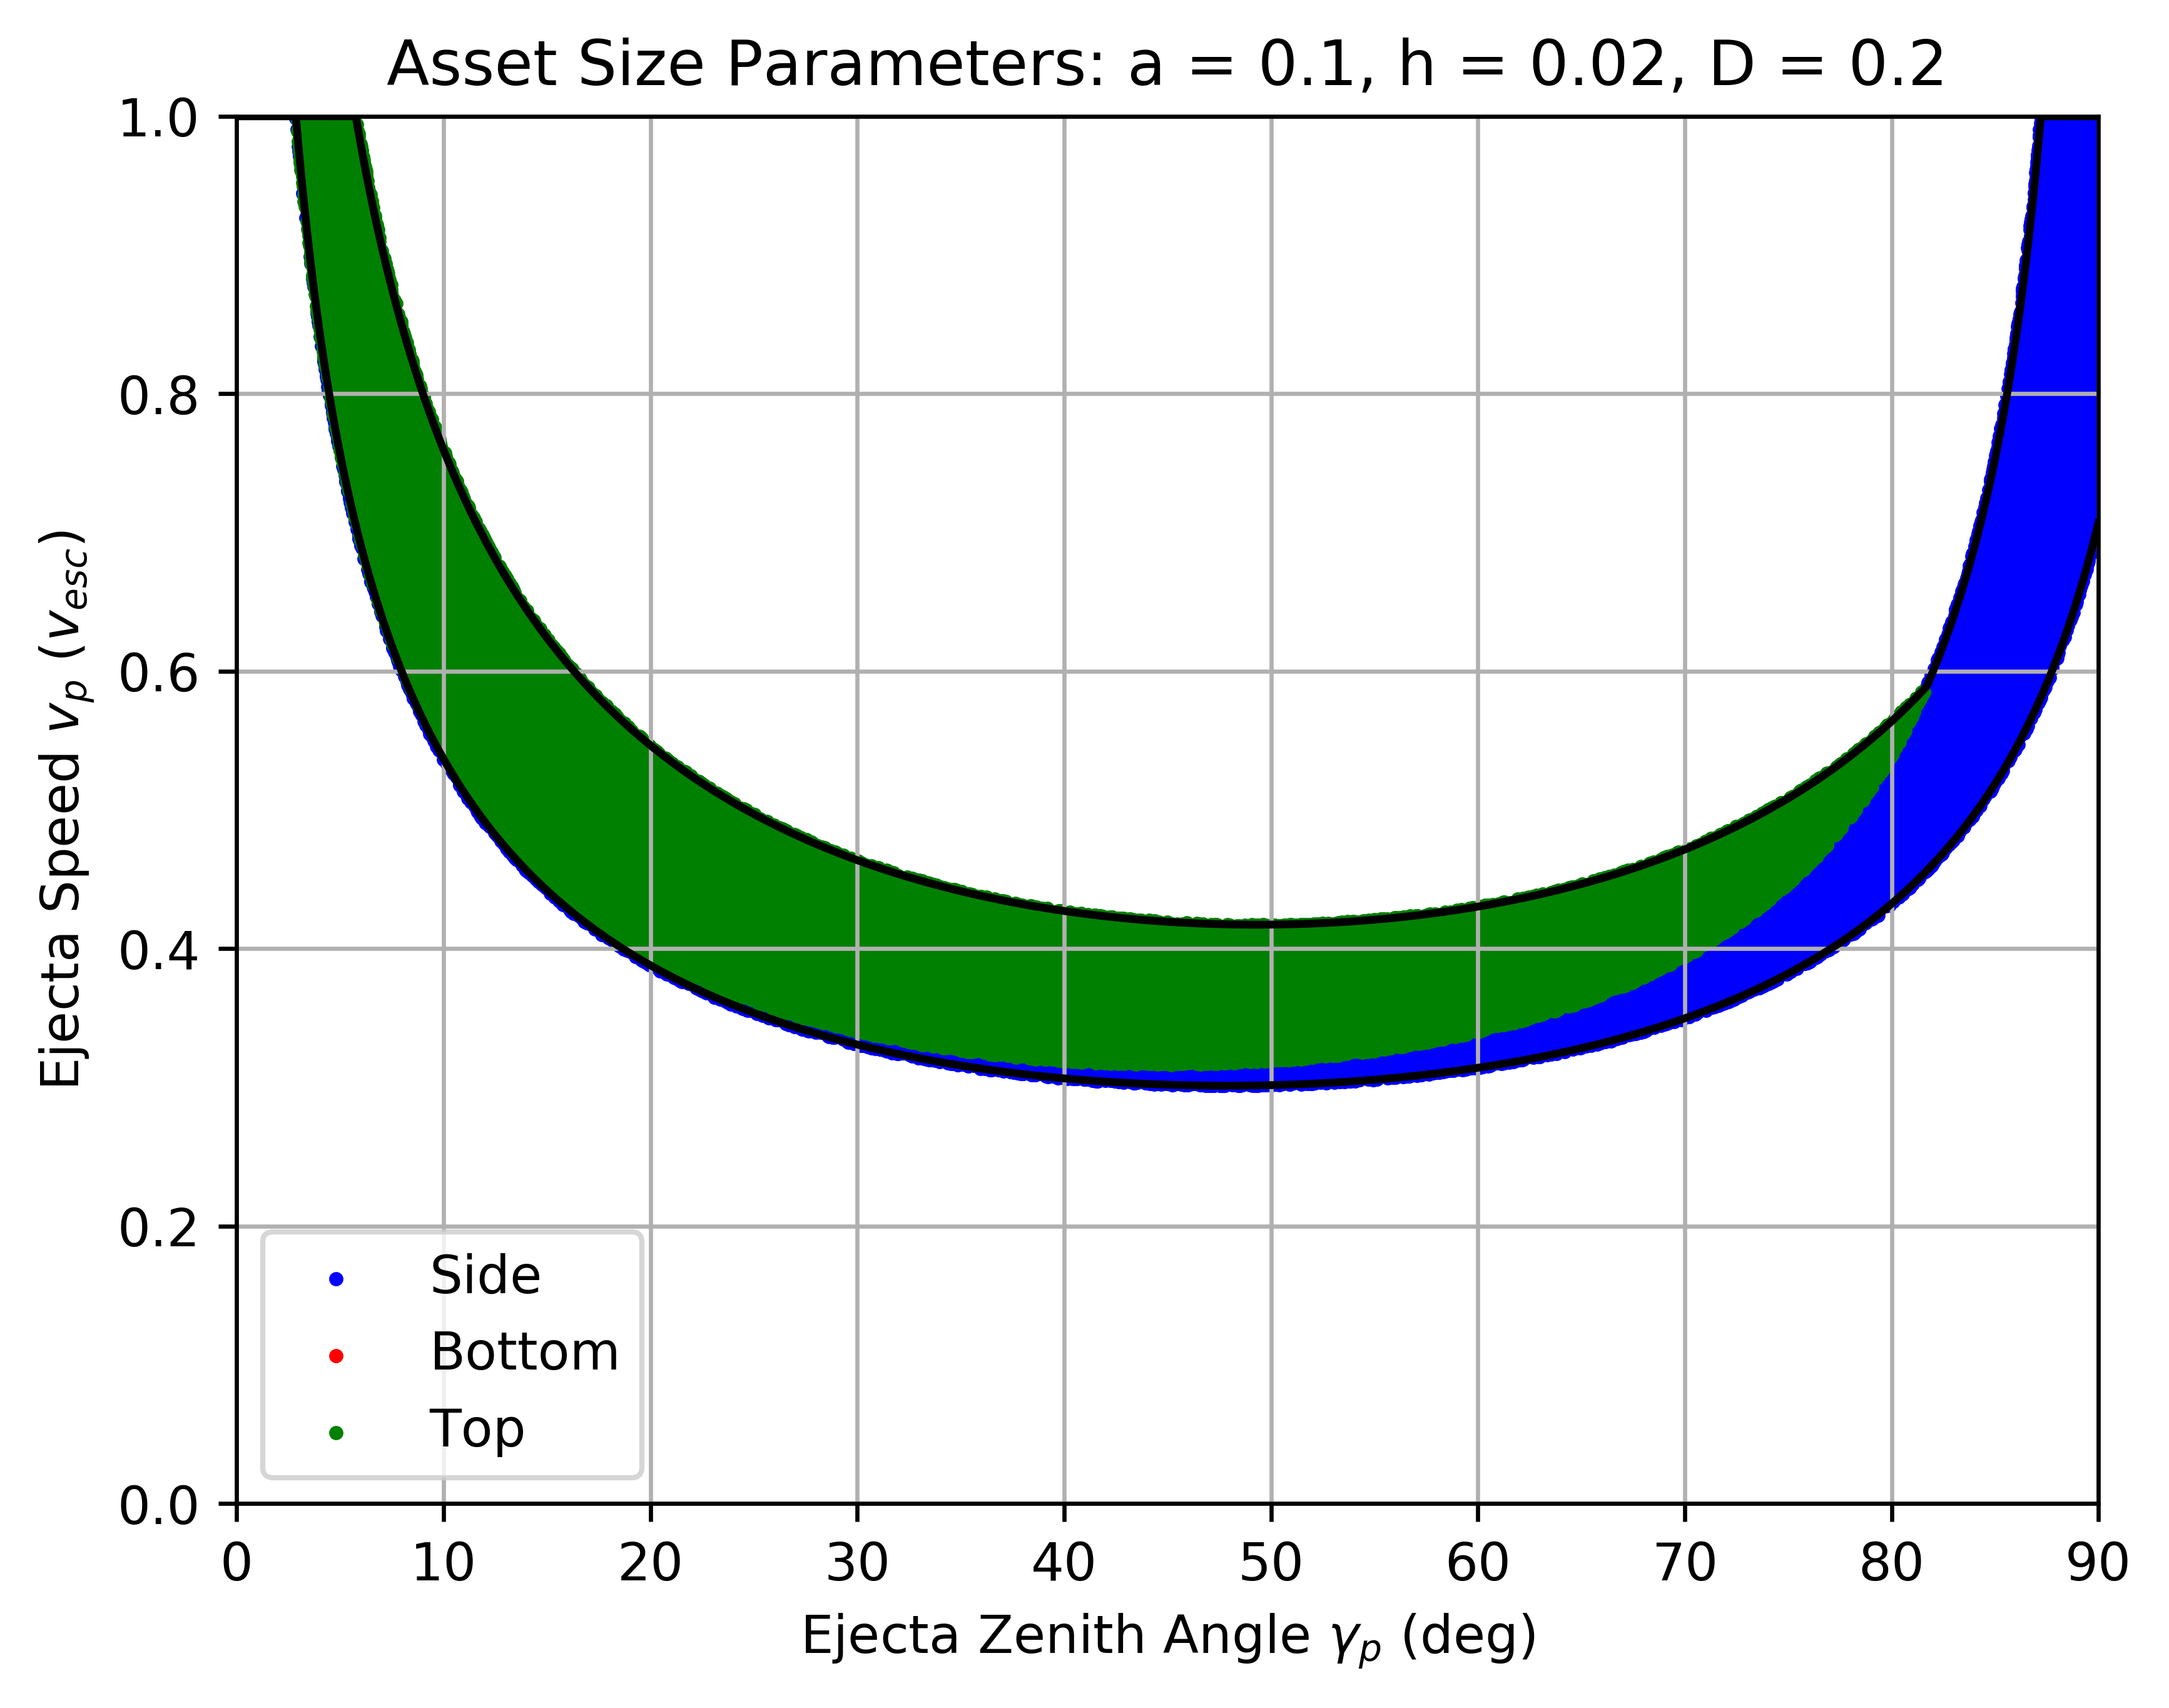
\includegraphics[width=.98\linewidth]{asset_speed_zenith_plot_1.000e-01_2.000e-02_2.000e-01.png}  
		%\caption{Put your sub-caption here}
		\label{fig:sub-asset_speed_zenith_9}
	\end{subfigure}
	
	\begin{subfigure}[t]{.32\textwidth}
		\centering
		% include third image
		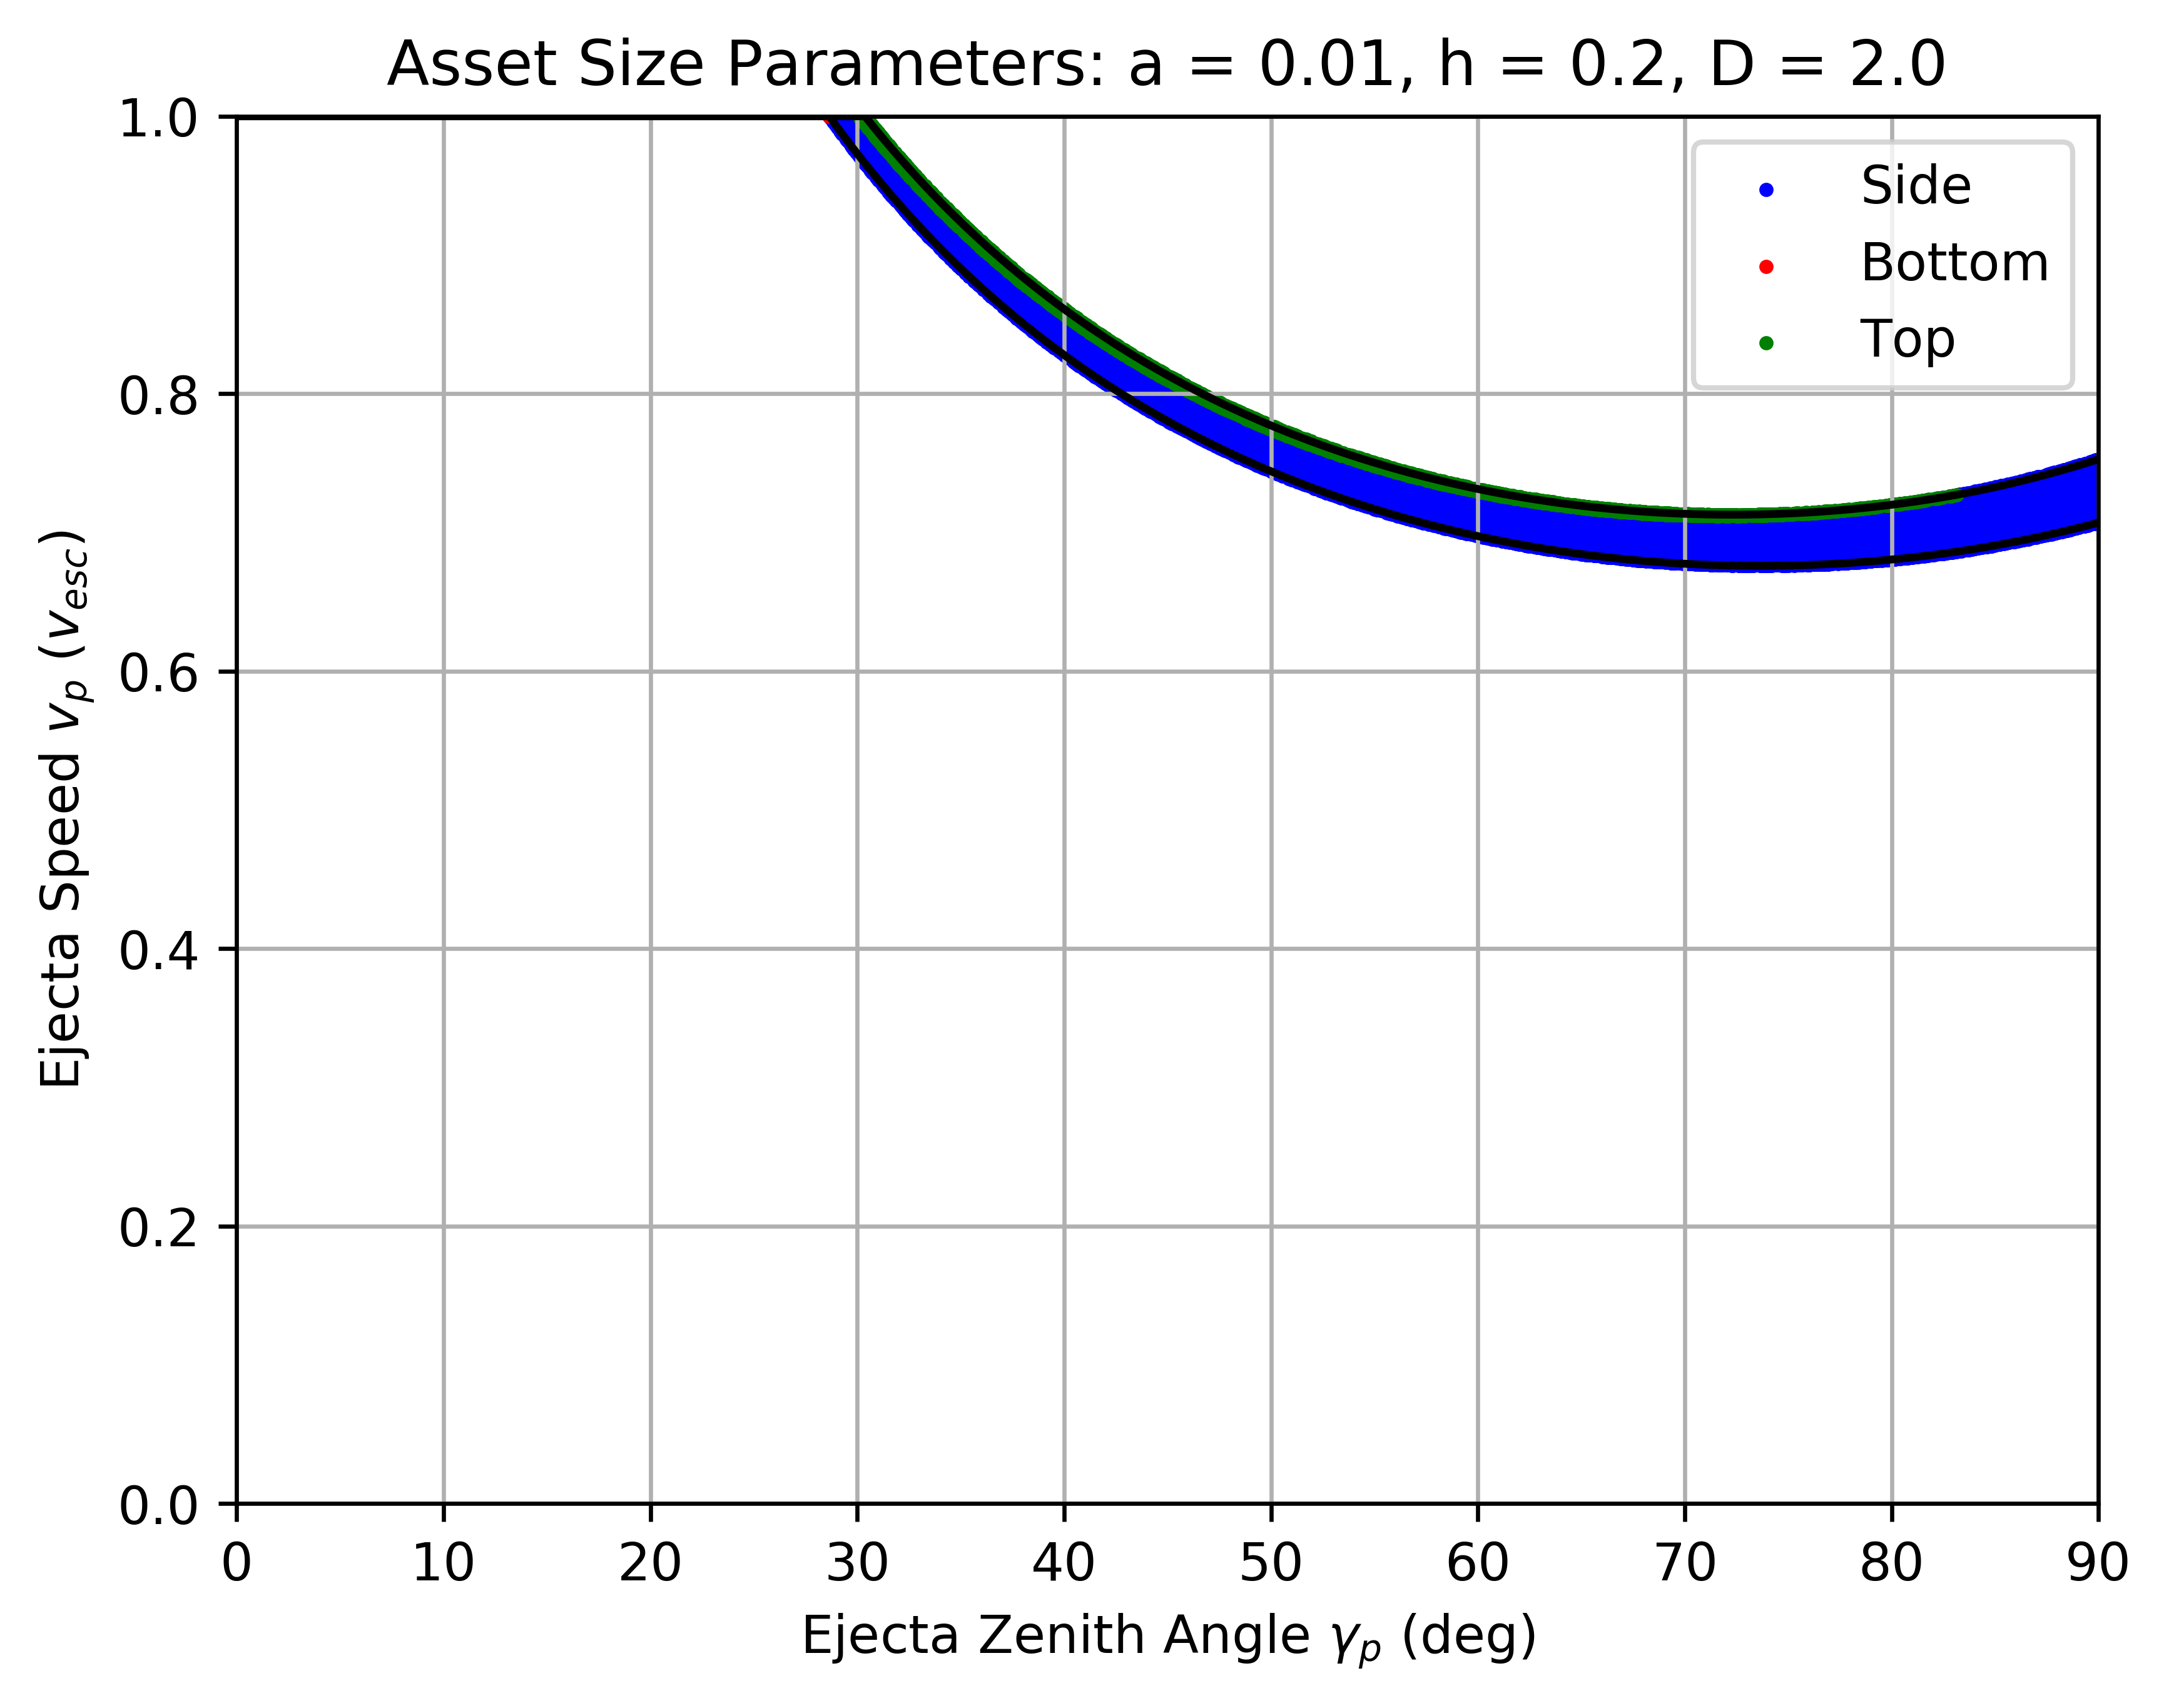
\includegraphics[width=.98\linewidth]{asset_speed_zenith_plot_1.000e-02_2.000e-01_2.000e+00.png}  
		%\caption{Put your sub-caption here}
		\label{fig:sub-asset_speed_zenith_10}
	\end{subfigure}
	\begin{subfigure}[t]{.32\textwidth}
		\centering
		% include fourth image
		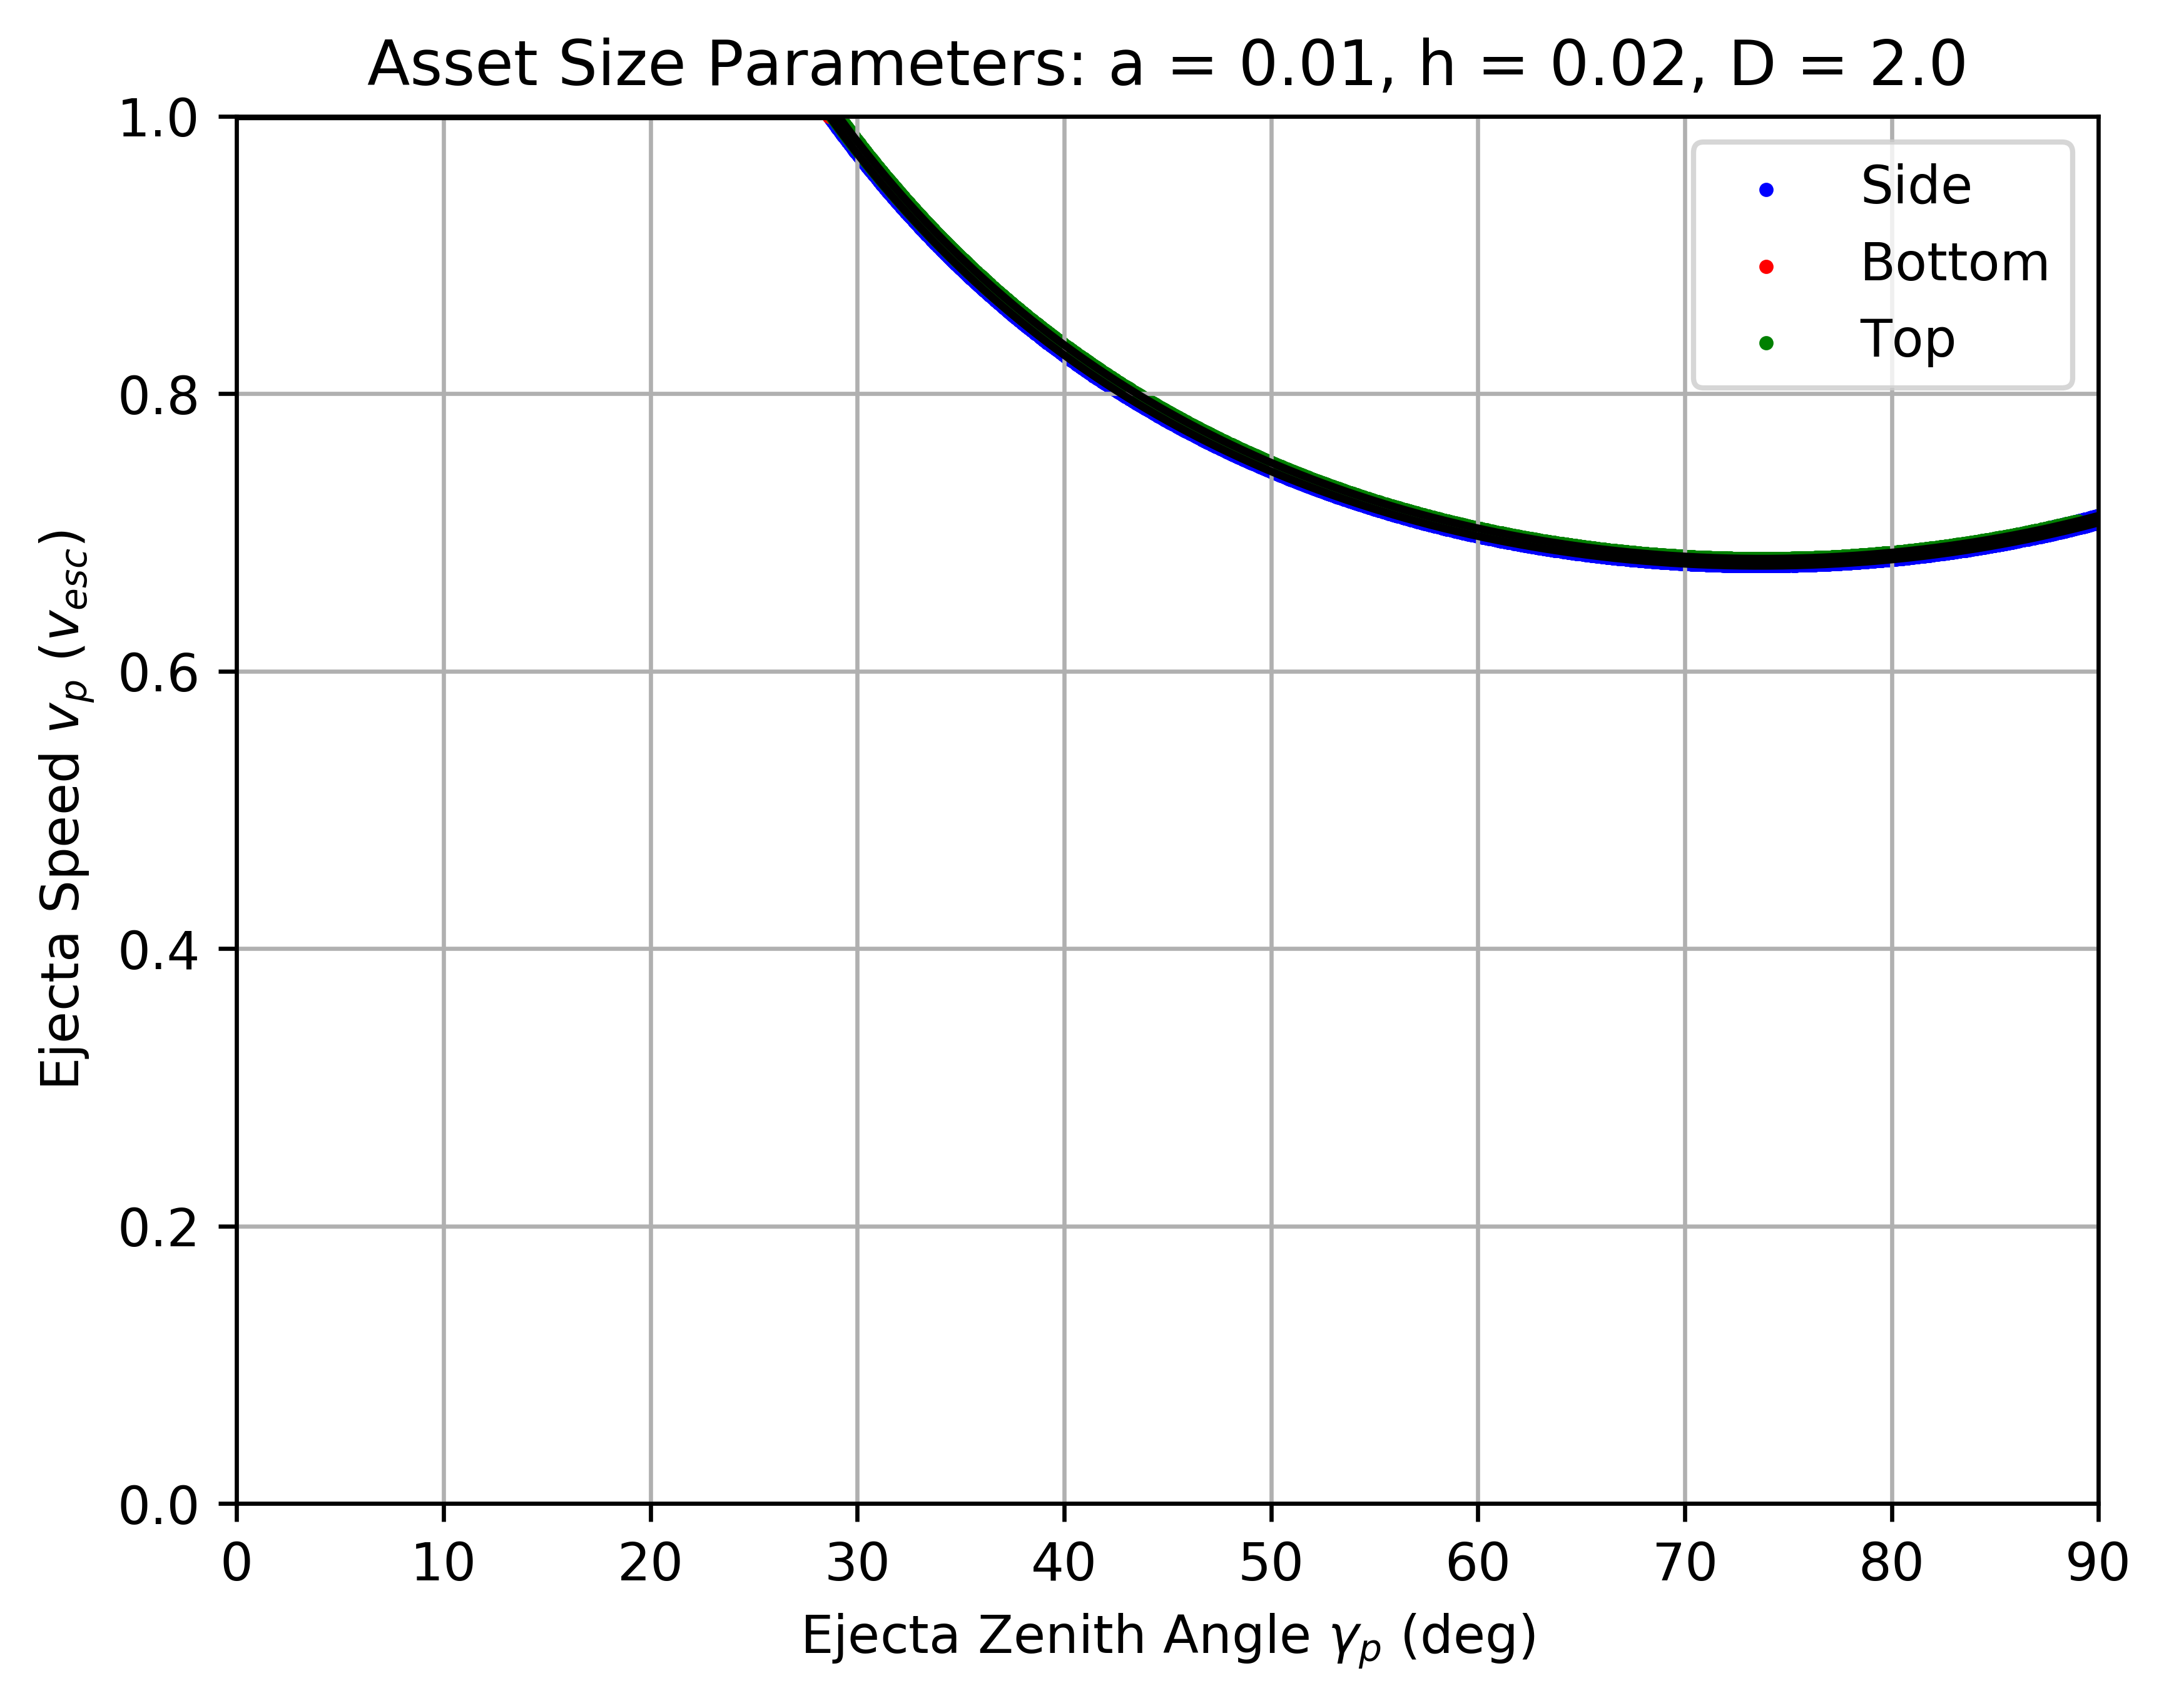
\includegraphics[width=.98\linewidth]{asset_speed_zenith_plot_1.000e-02_2.000e-02_2.000e+00.png}  
		%\caption{Put your sub-caption here}
		\label{fig:sub-asset_speed_zenith_11}
	\end{subfigure}
	\begin{subfigure}[t]{.32\textwidth}
		\centering
		% include fourth image
		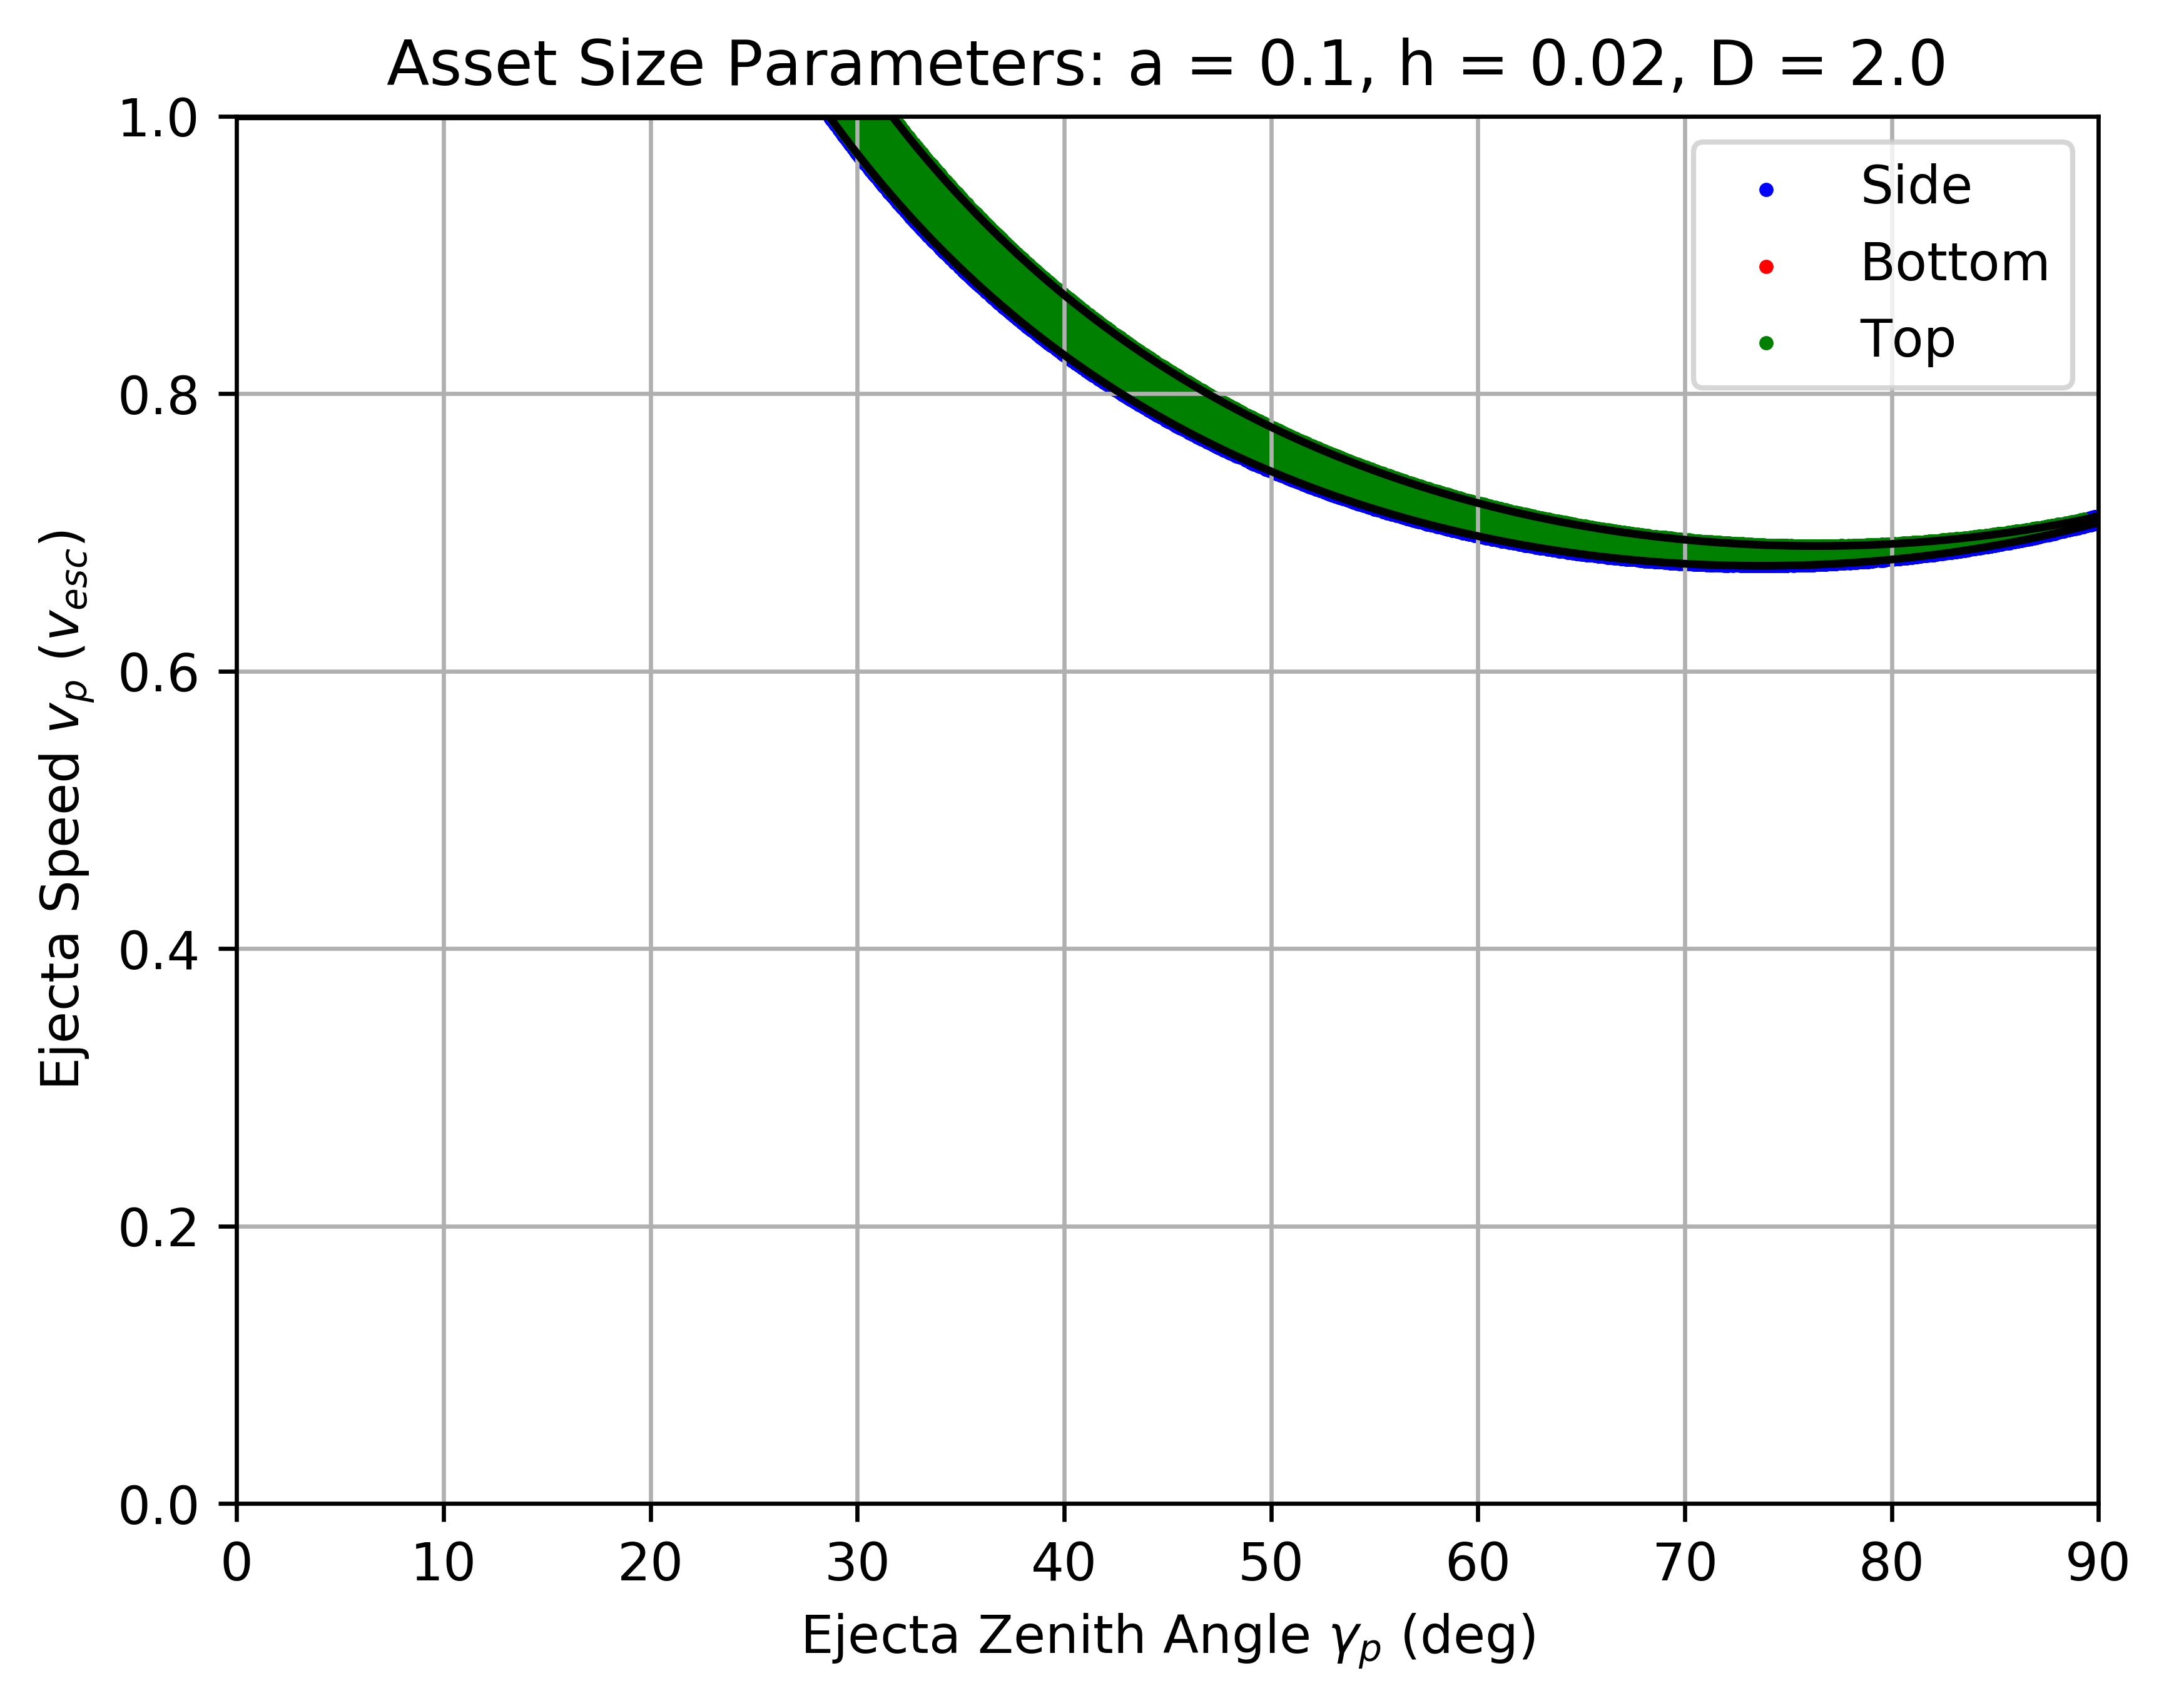
\includegraphics[width=.98\linewidth]{asset_speed_zenith_plot_1.000e-01_2.000e-02_2.000e+00.png}  
		%\caption{Put your sub-caption here}
		\label{fig:sub-asset_speed_zenith_12}
	\end{subfigure}
	
	\caption{A matrix of plots showing the ejecta hitting a cylindrical asset (in a plane intersecting the cylinder's symmetry axis) on the surface for various asset sizes and crater-to-asset distances. Each plot gives three colors for the ejecta hitting the side (blue), bottom (red), and the top (green) as a function of initial ejecta speed $v_p$ vs.\ initial ejecta zenith angle $\gamma_p$.}
	\label{fig:asset_speed_zenith_comparison}
\end{figure}









\begin{figure}
	\begin{subfigure}[t]{.32\textwidth}
		\centering
		% include first image
		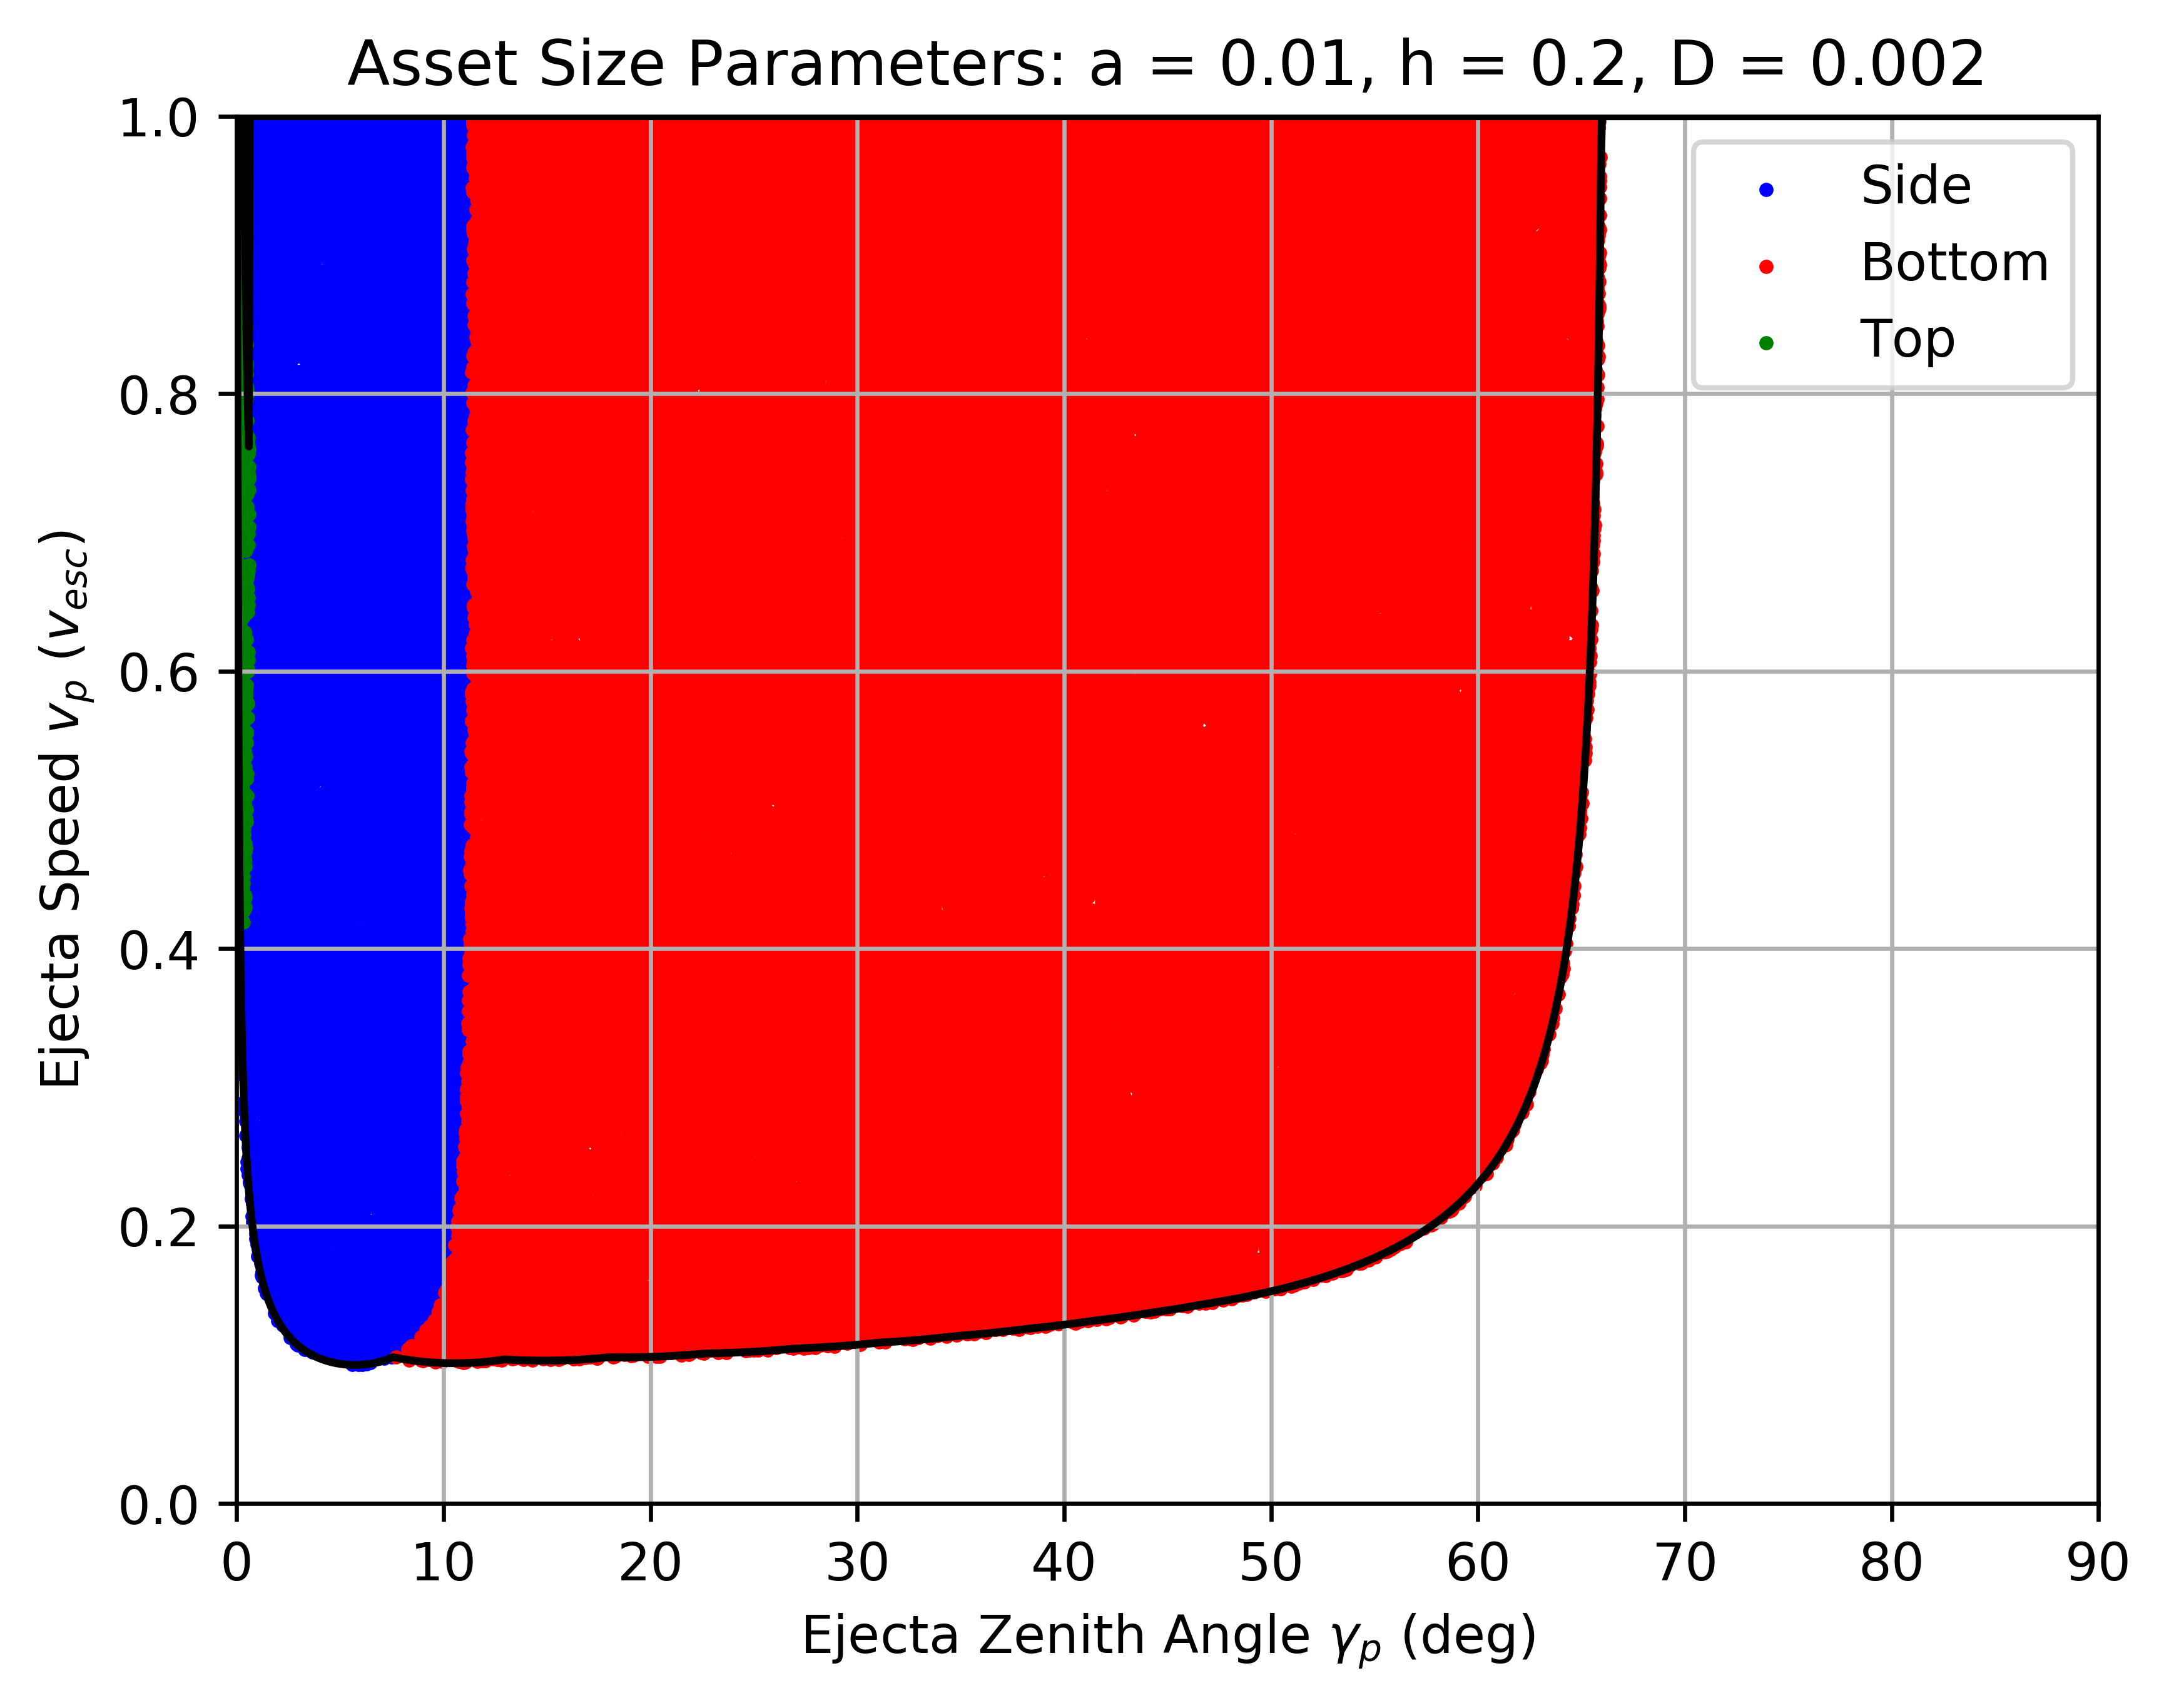
\includegraphics[width=.98\linewidth]{asset_speed_zenith_plot_1.010e+00_1.000e-02_2.000e-01_2.000e-03.png}  
		%\caption{Put your sub-caption here}
		\label{fig:sub-asset_speed_zenith_h1_1}
	\end{subfigure}
	\begin{subfigure}[t]{.32\textwidth}
		\centering
		% include second image
		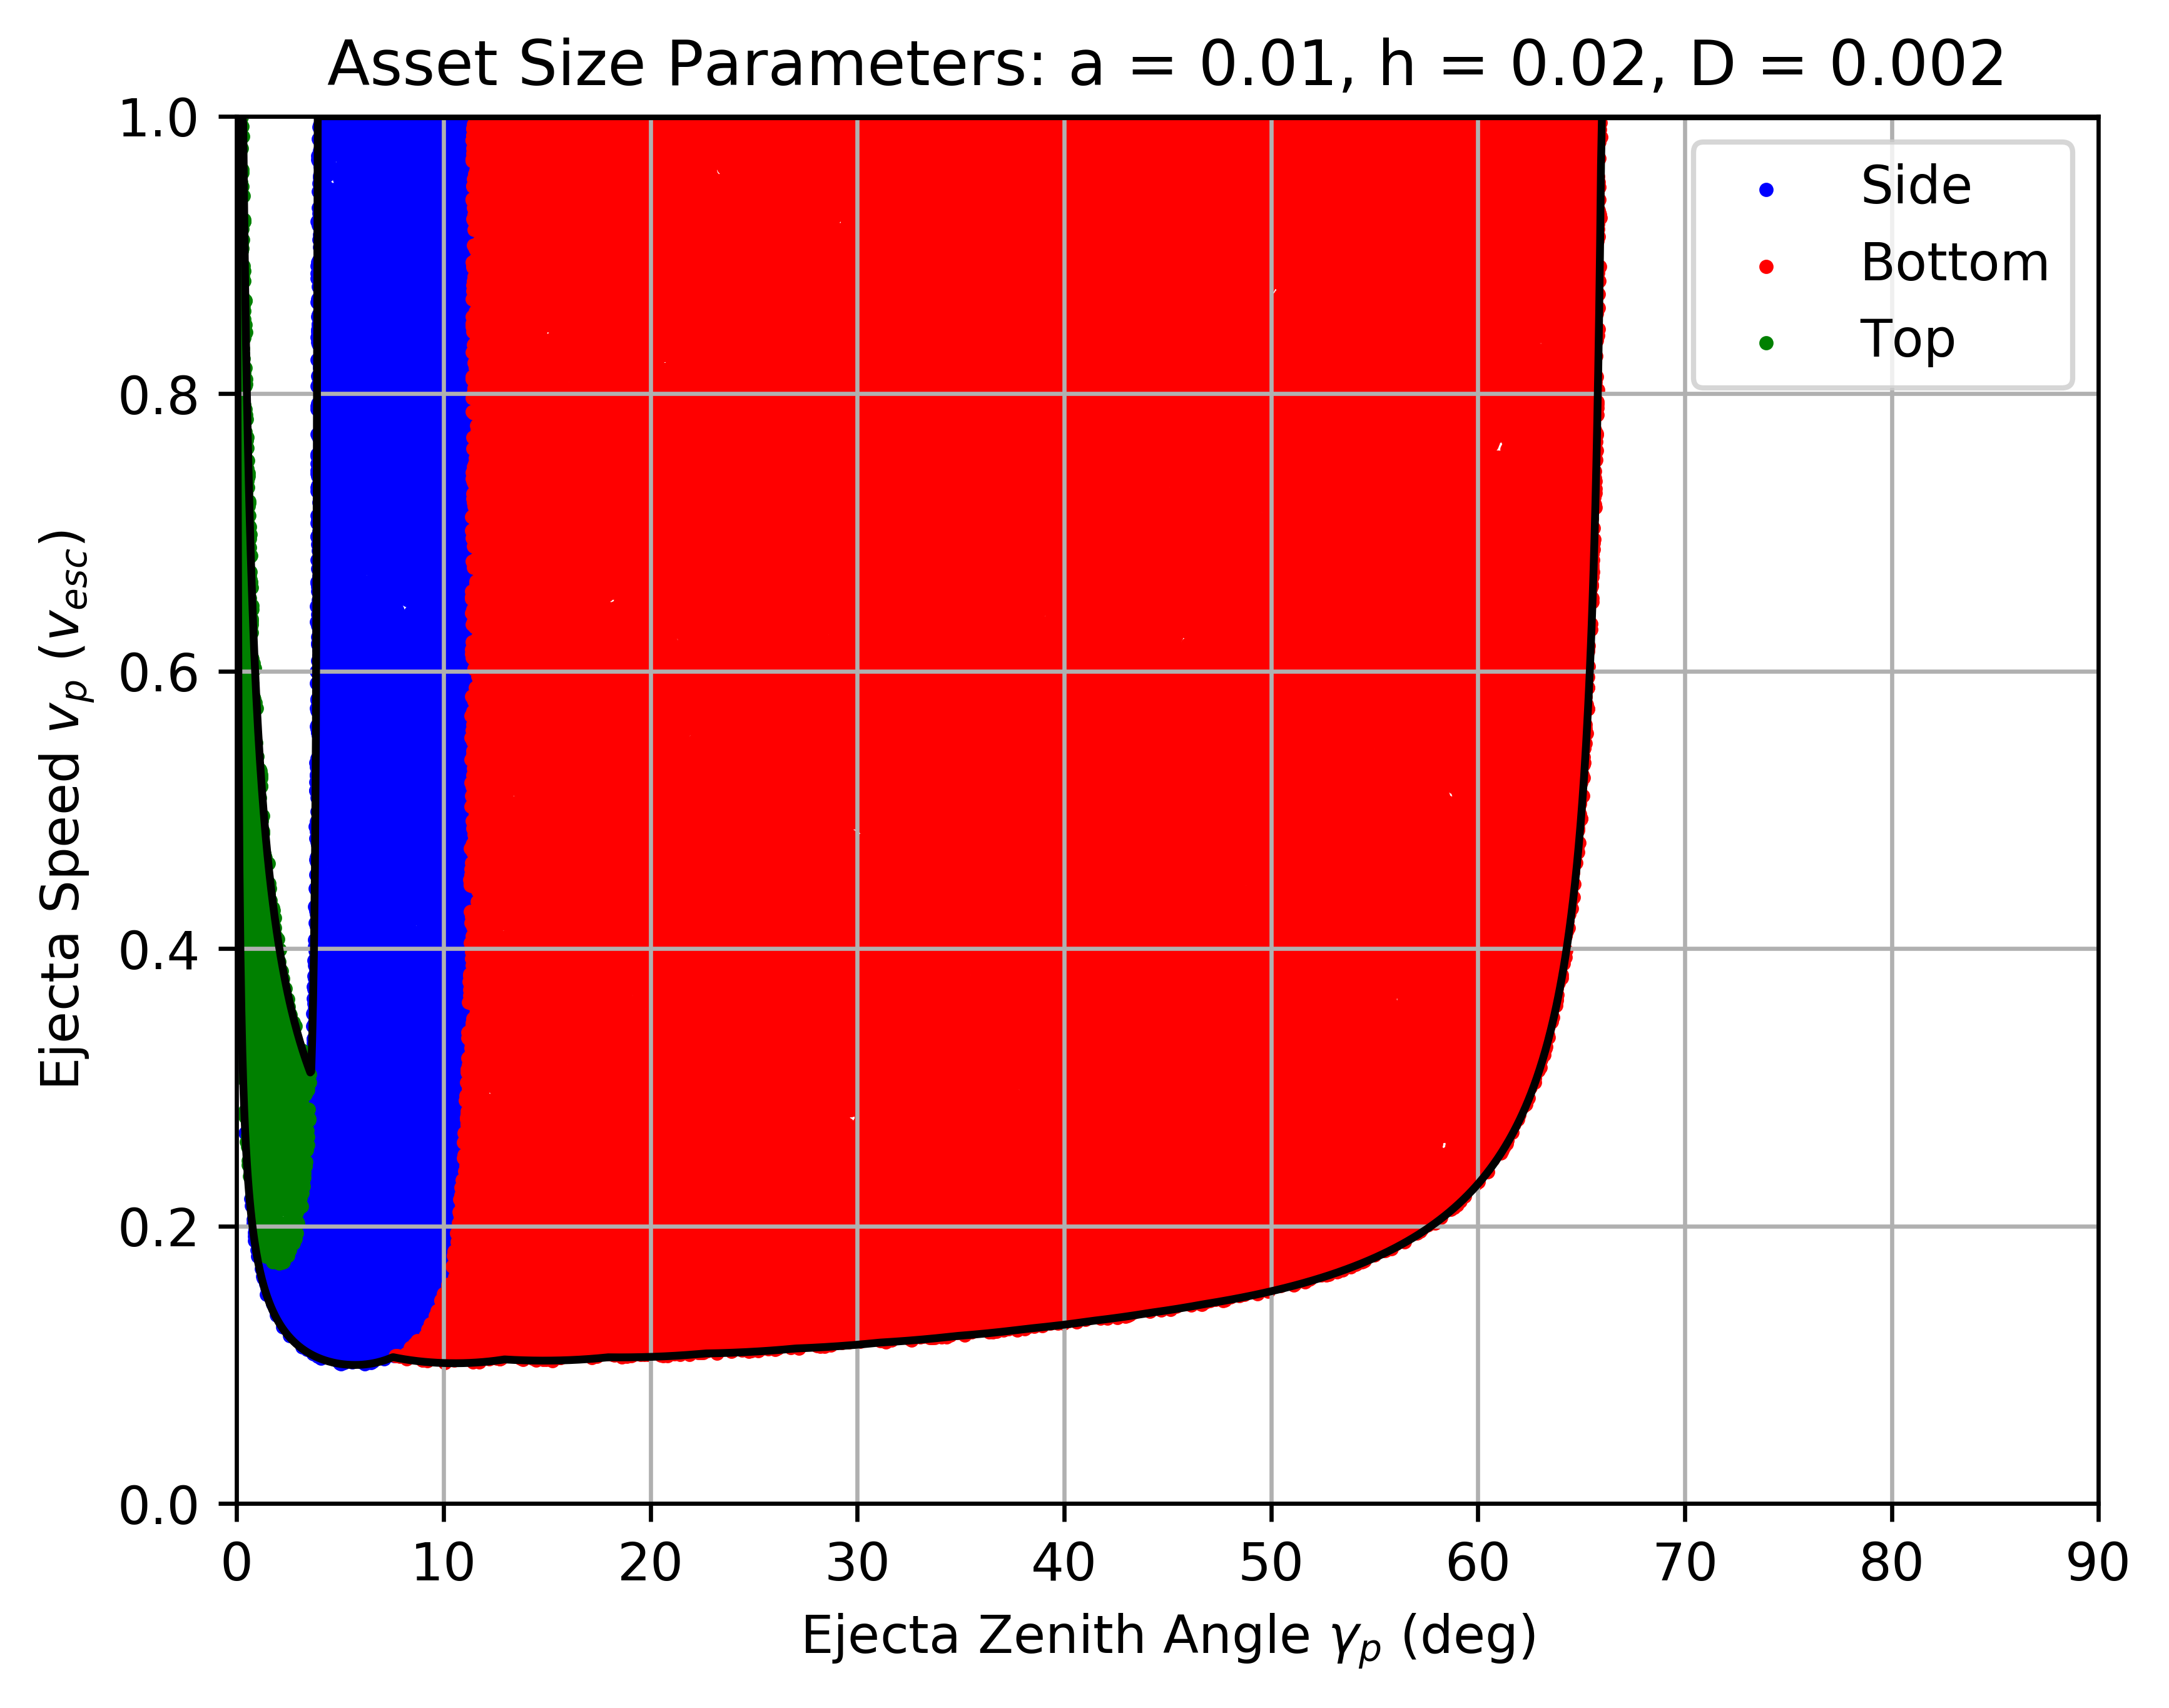
\includegraphics[width=.98\linewidth]{asset_speed_zenith_plot_1.010e+00_1.000e-02_2.000e-02_2.000e-03.png}  
		%\caption{Put your sub-caption here}
		\label{fig:sub-asset_speed_zenith_h1_2}
	\end{subfigure}
	\begin{subfigure}[t]{.32\textwidth}
		\centering
		% include second image
		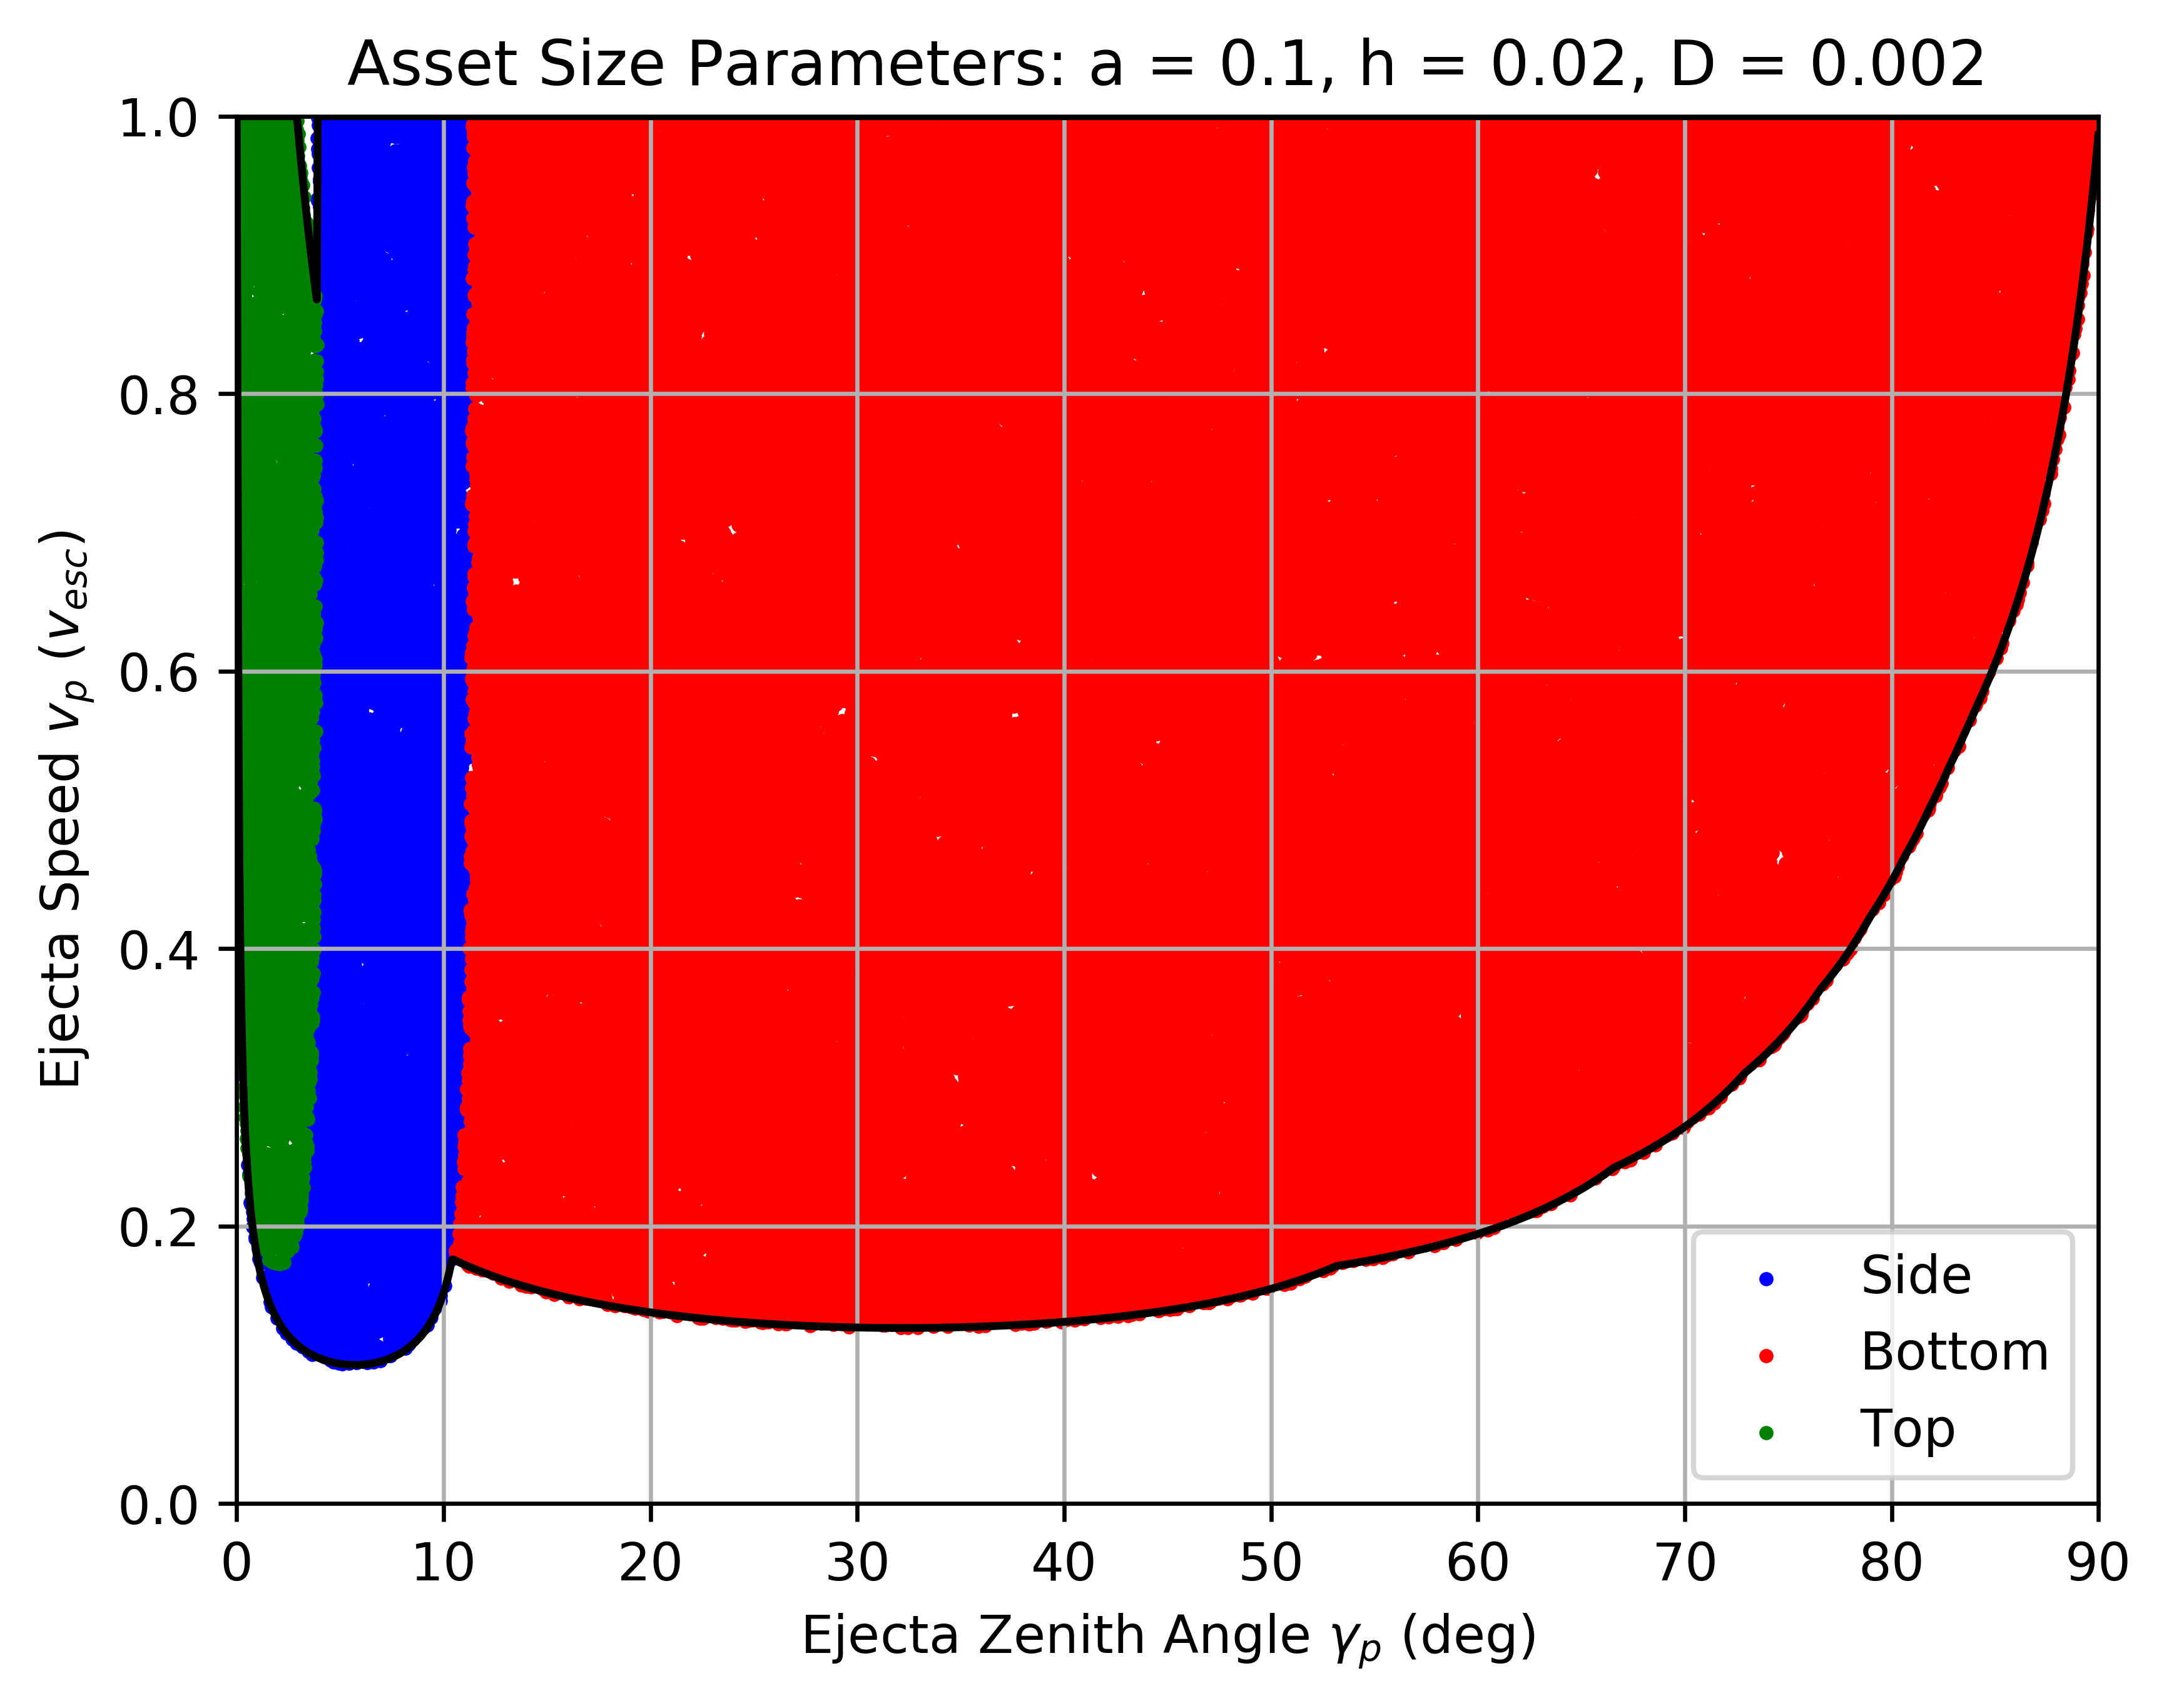
\includegraphics[width=.98\linewidth]{asset_speed_zenith_plot_1.010e+00_1.000e-01_2.000e-02_2.000e-03.png}  
		%\caption{Put your sub-caption here}
		\label{fig:sub-asset_speed_zenith_h1_3}
	\end{subfigure}
	
	%\newline
	
	\begin{subfigure}[t]{.32\textwidth}
		\centering
		% include third image
		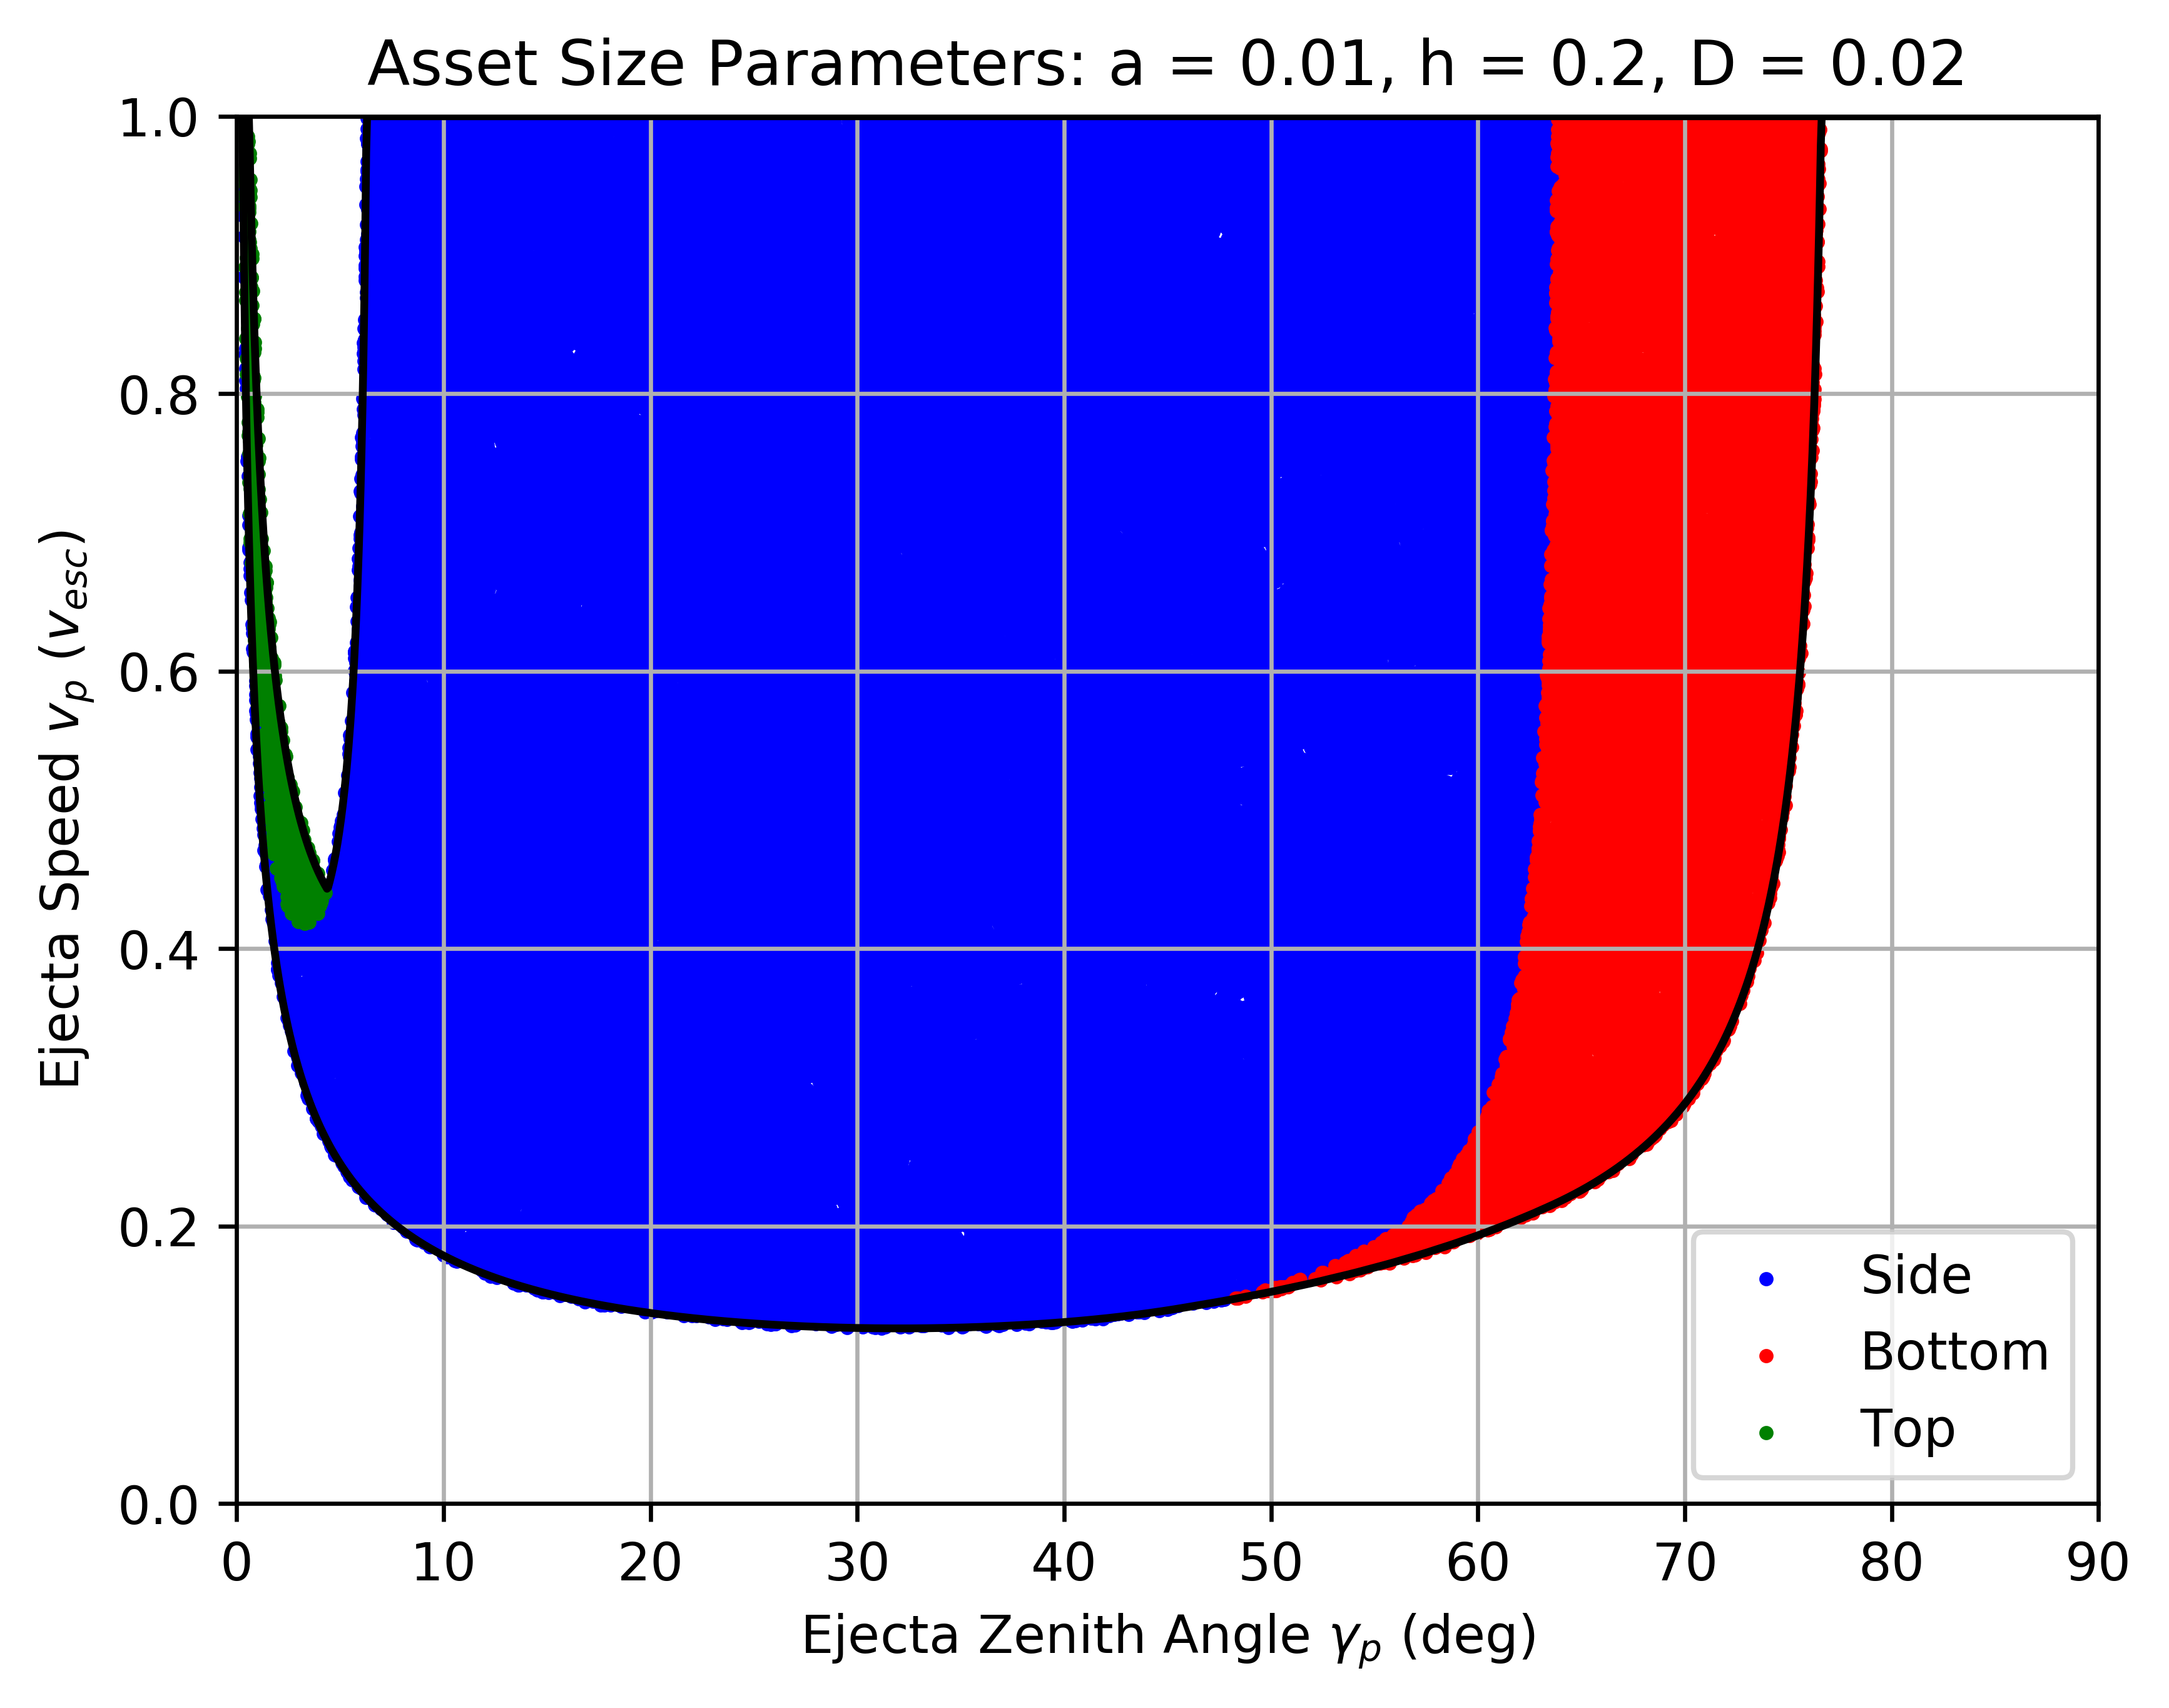
\includegraphics[width=.98\linewidth]{asset_speed_zenith_plot_1.010e+00_1.000e-02_2.000e-01_2.000e-02.png}  
		%\caption{Put your sub-caption here}
		\label{fig:sub-asset_speed_zenith_h1_4}
	\end{subfigure}
	\begin{subfigure}[t]{.32\textwidth}
		\centering
		% include fourth image
		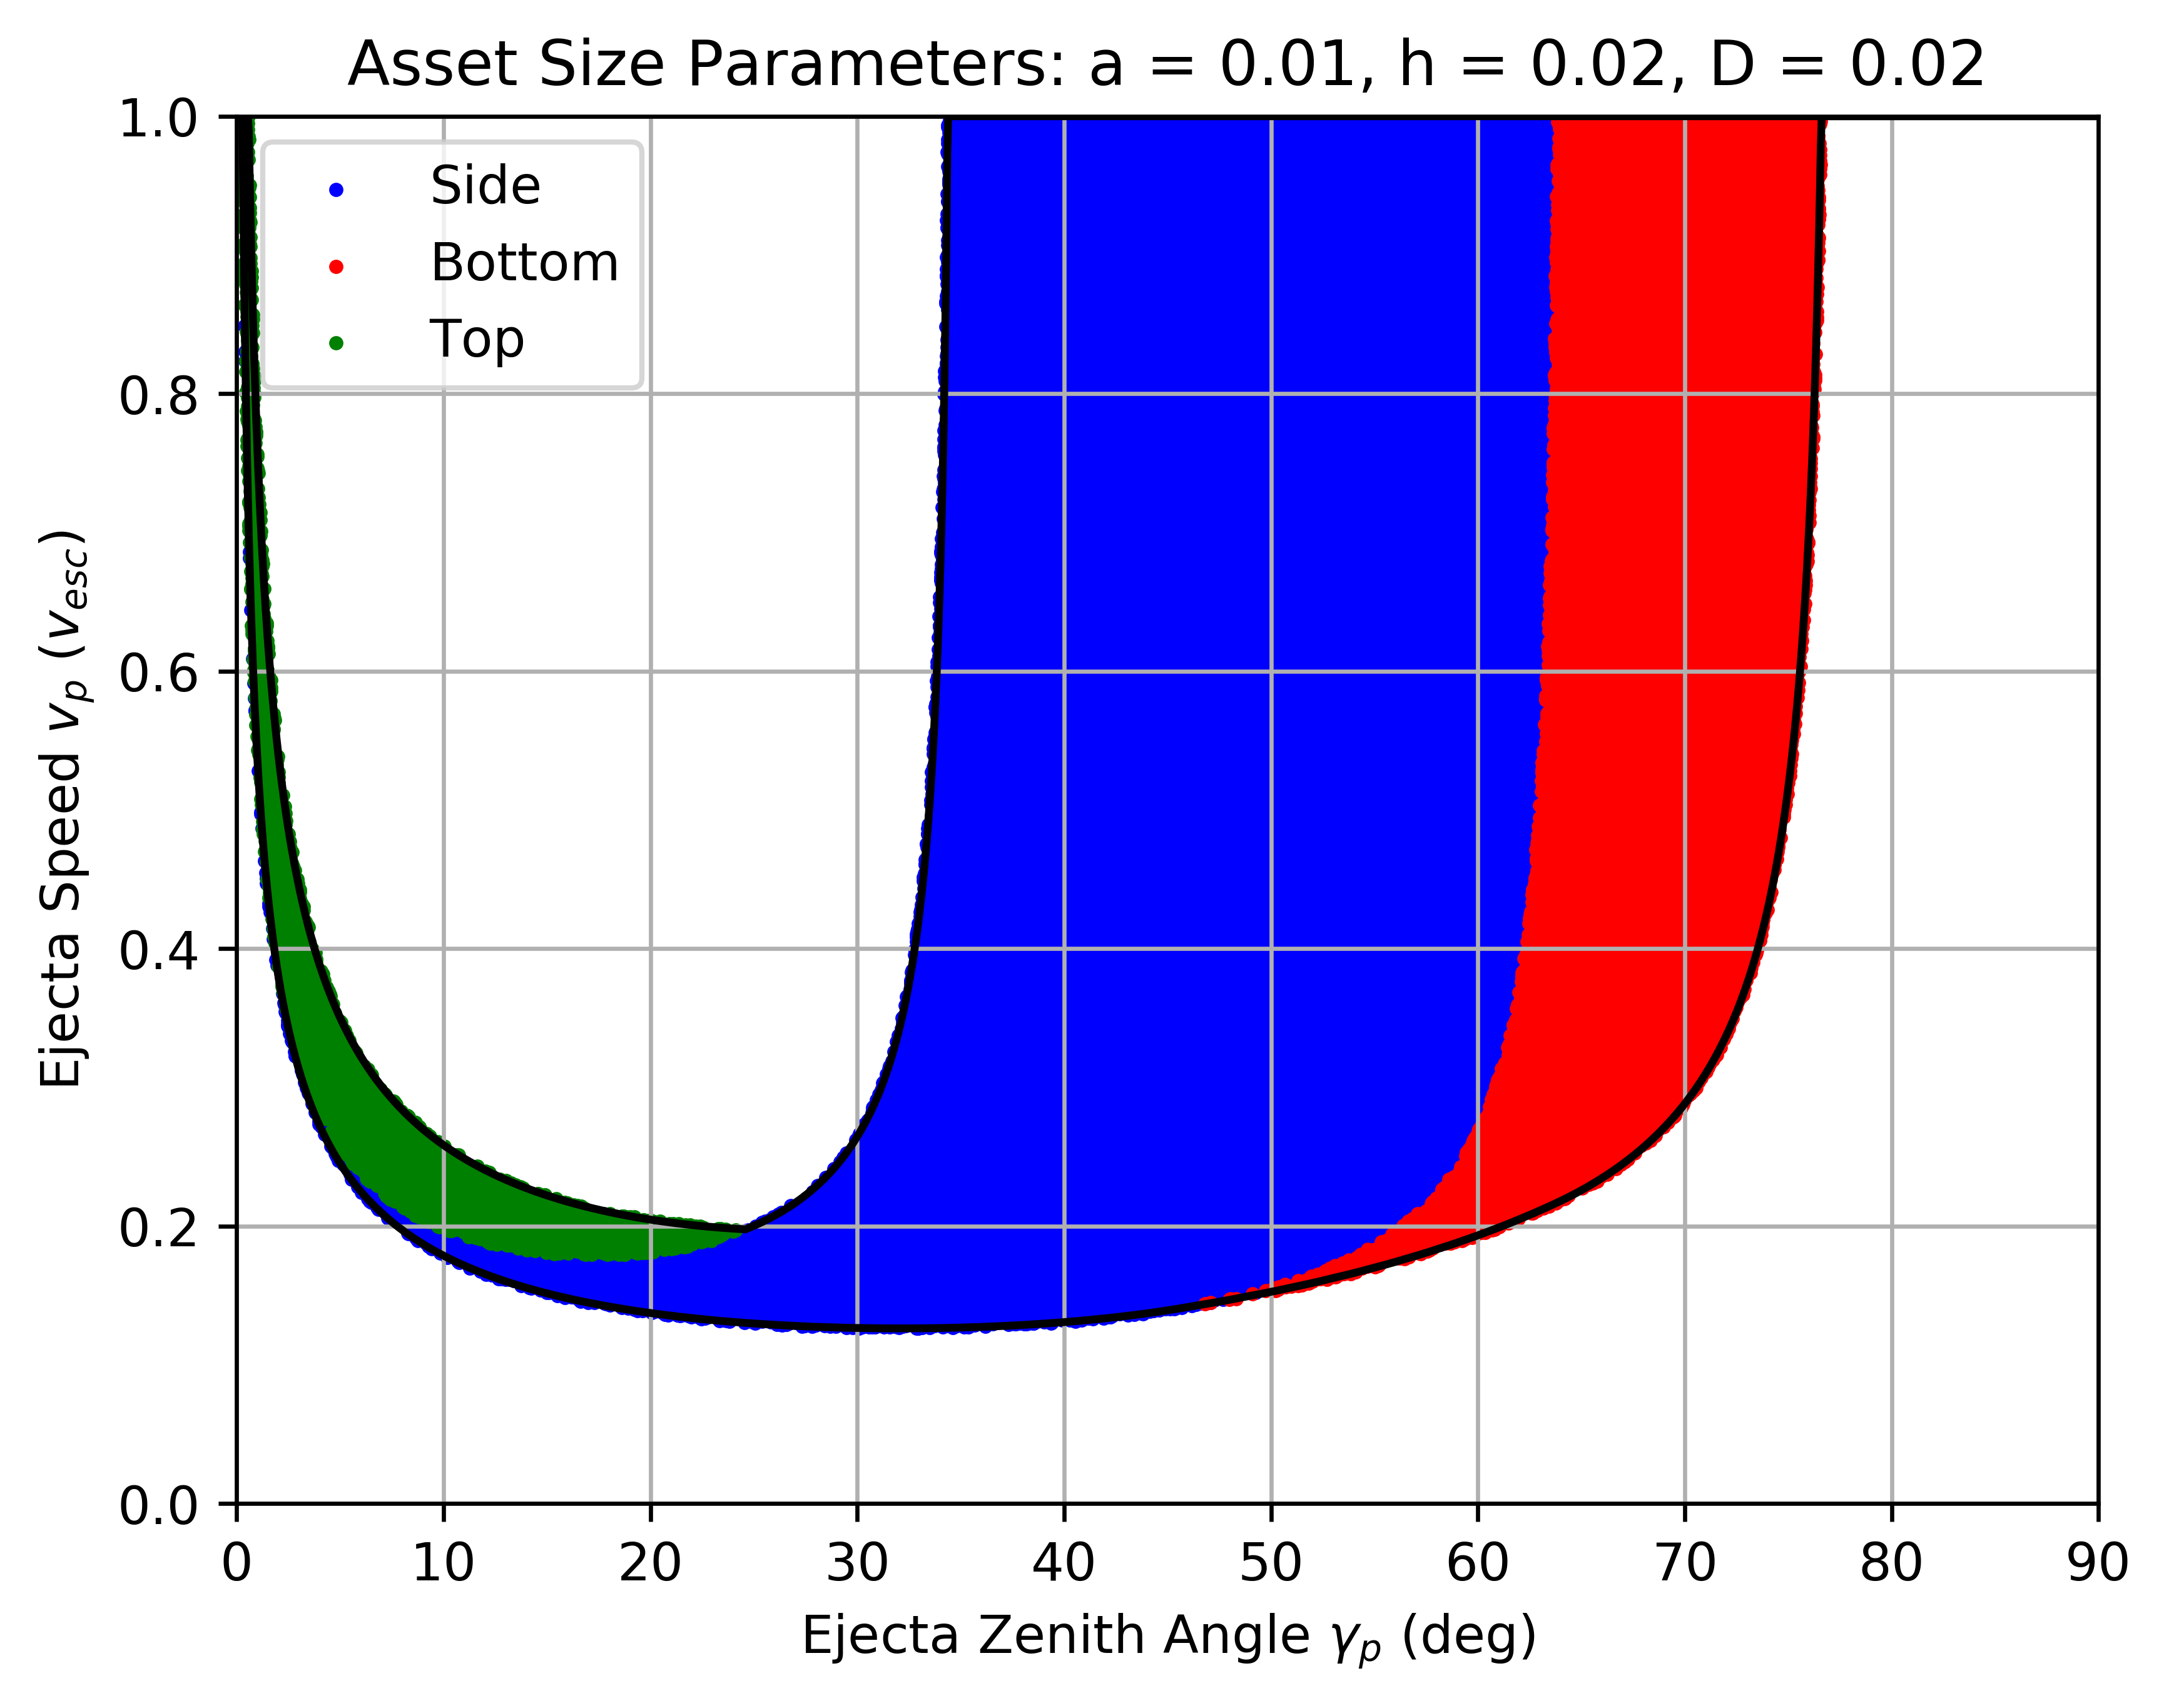
\includegraphics[width=.98\linewidth]{asset_speed_zenith_plot_1.010e+00_1.000e-02_2.000e-02_2.000e-02.png}  
		%\caption{Put your sub-caption here}
		\label{fig:sub-asset_speed_zenith_h1_5}
	\end{subfigure}
	\begin{subfigure}[t]{.32\textwidth}
		\centering
		% include fourth image
		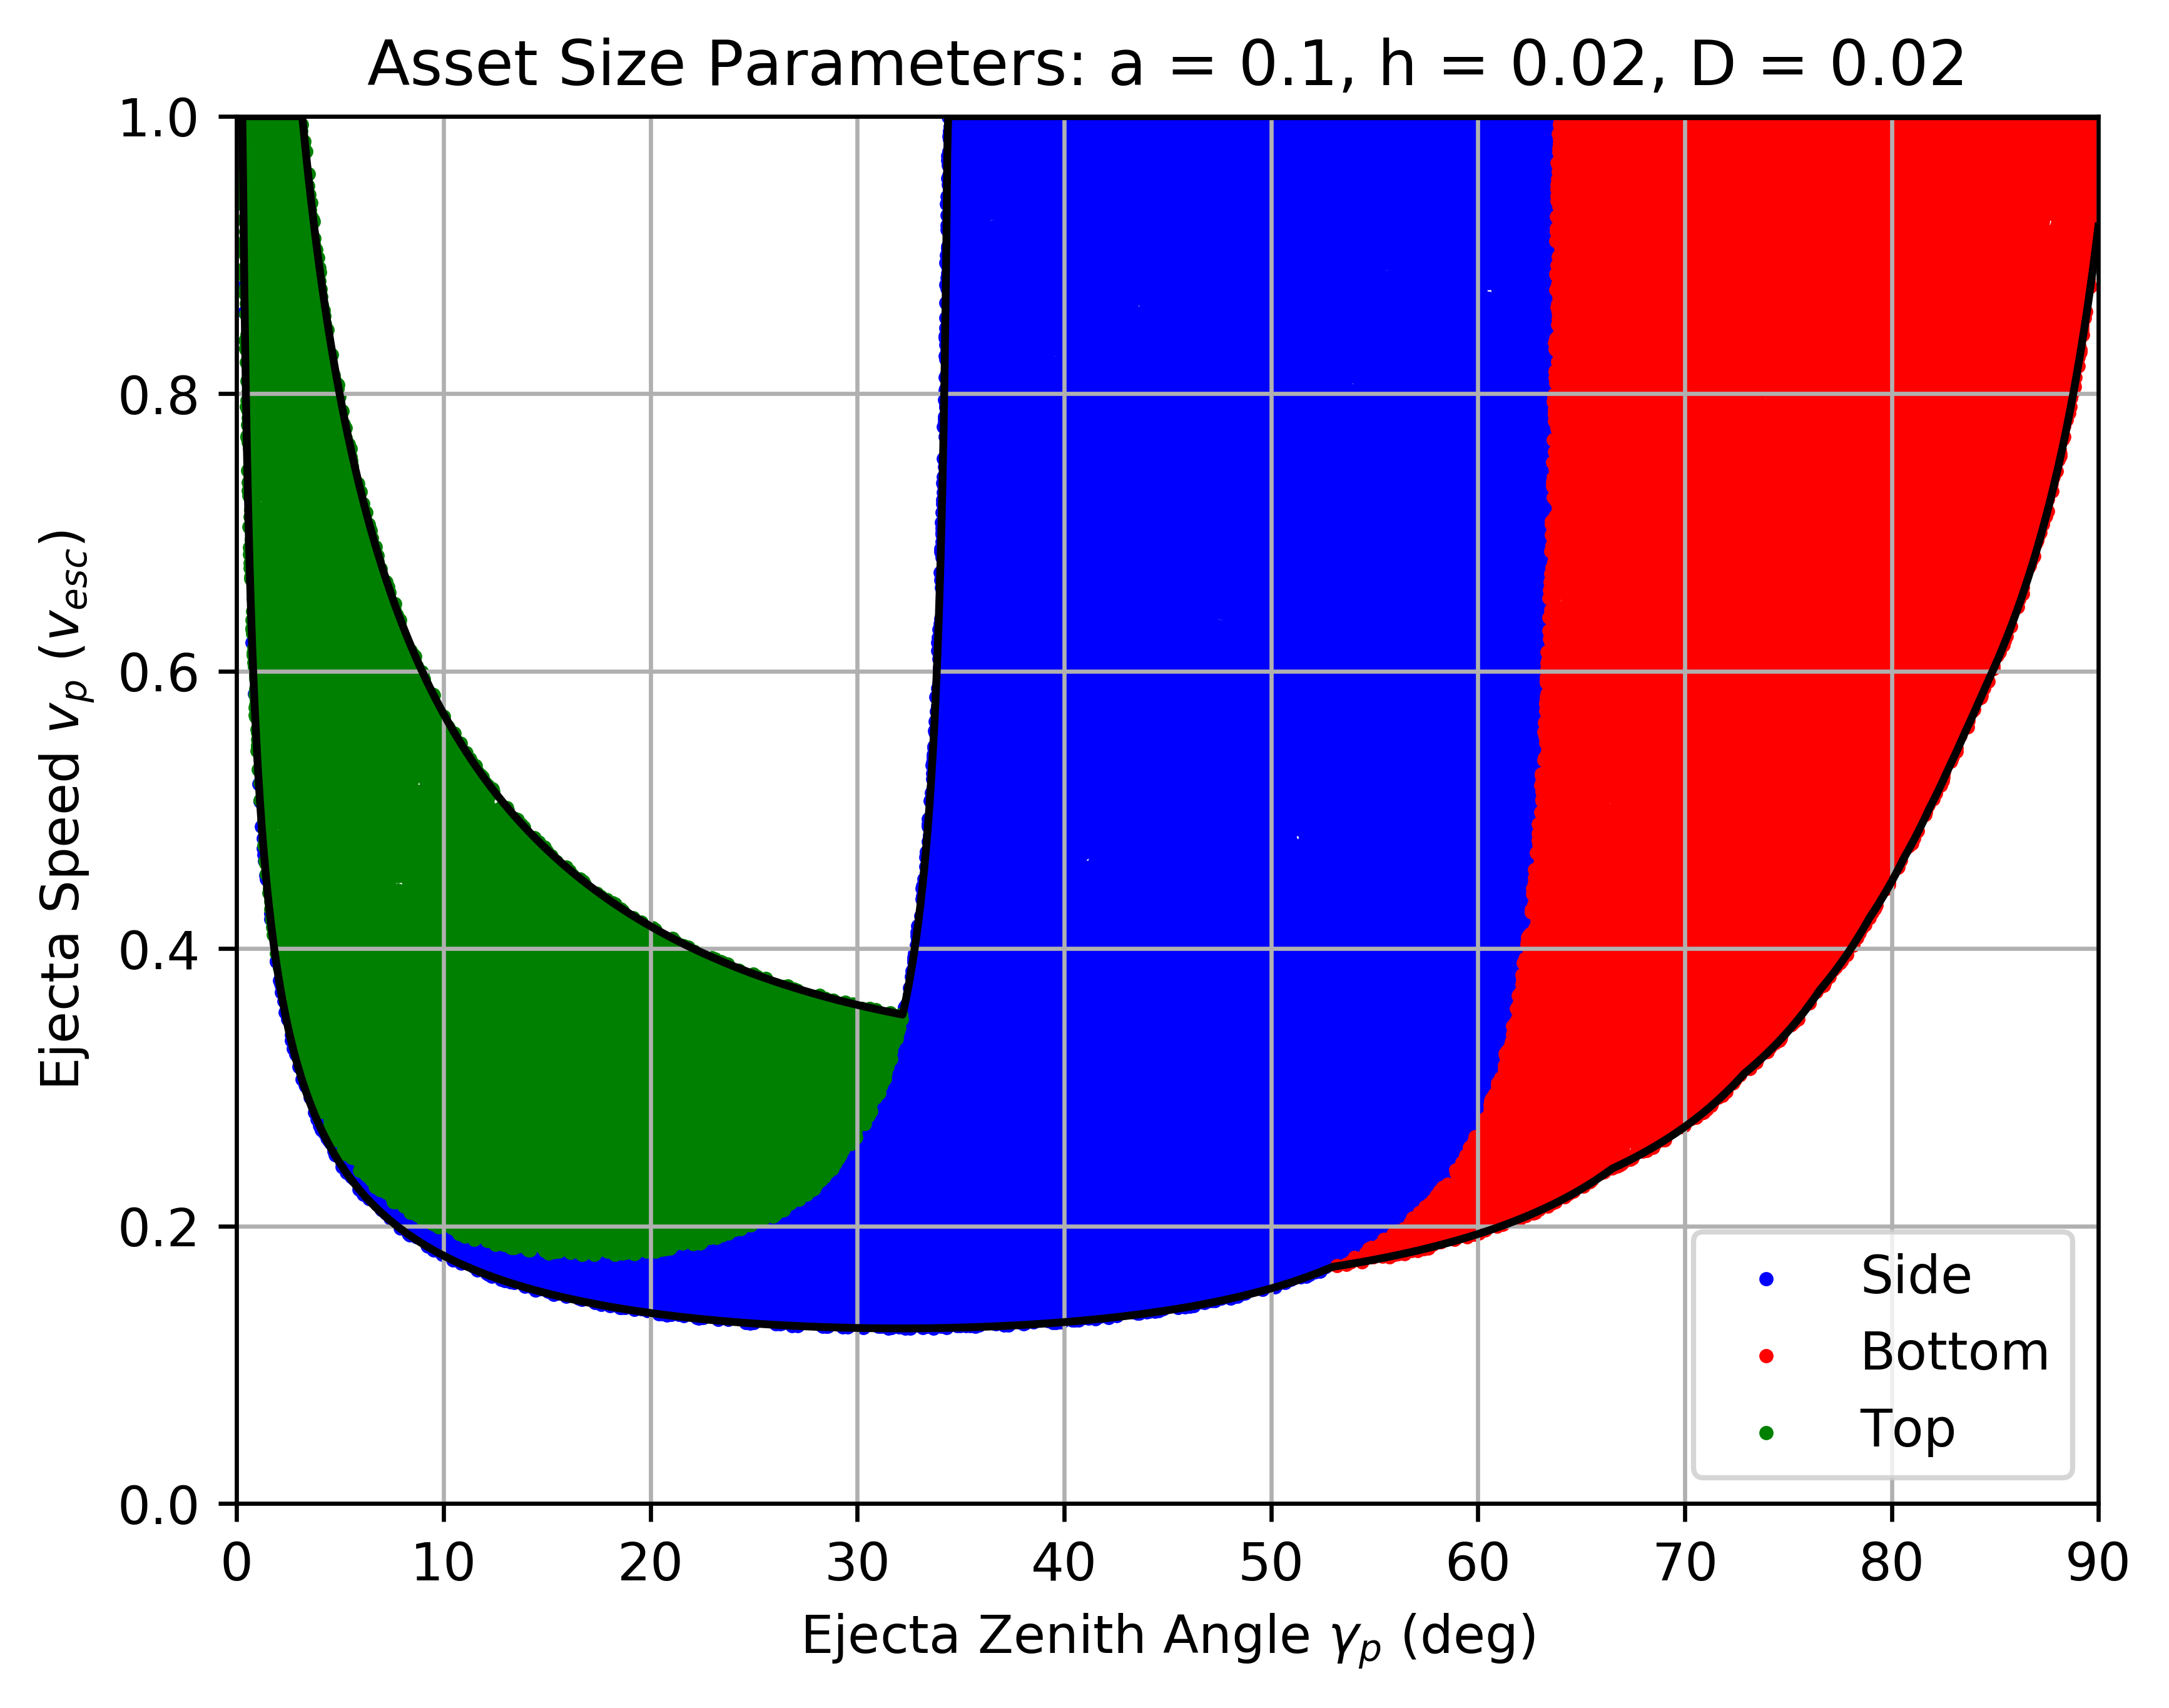
\includegraphics[width=.98\linewidth]{asset_speed_zenith_plot_1.010e+00_1.000e-01_2.000e-02_2.000e-02.png}  
		%\caption{Put your sub-caption here}
		\label{fig:sub-asset_speed_zenith_h1_6}
	\end{subfigure}
	
	
	\begin{subfigure}[t]{.32\textwidth}
		\centering
		% include third image
		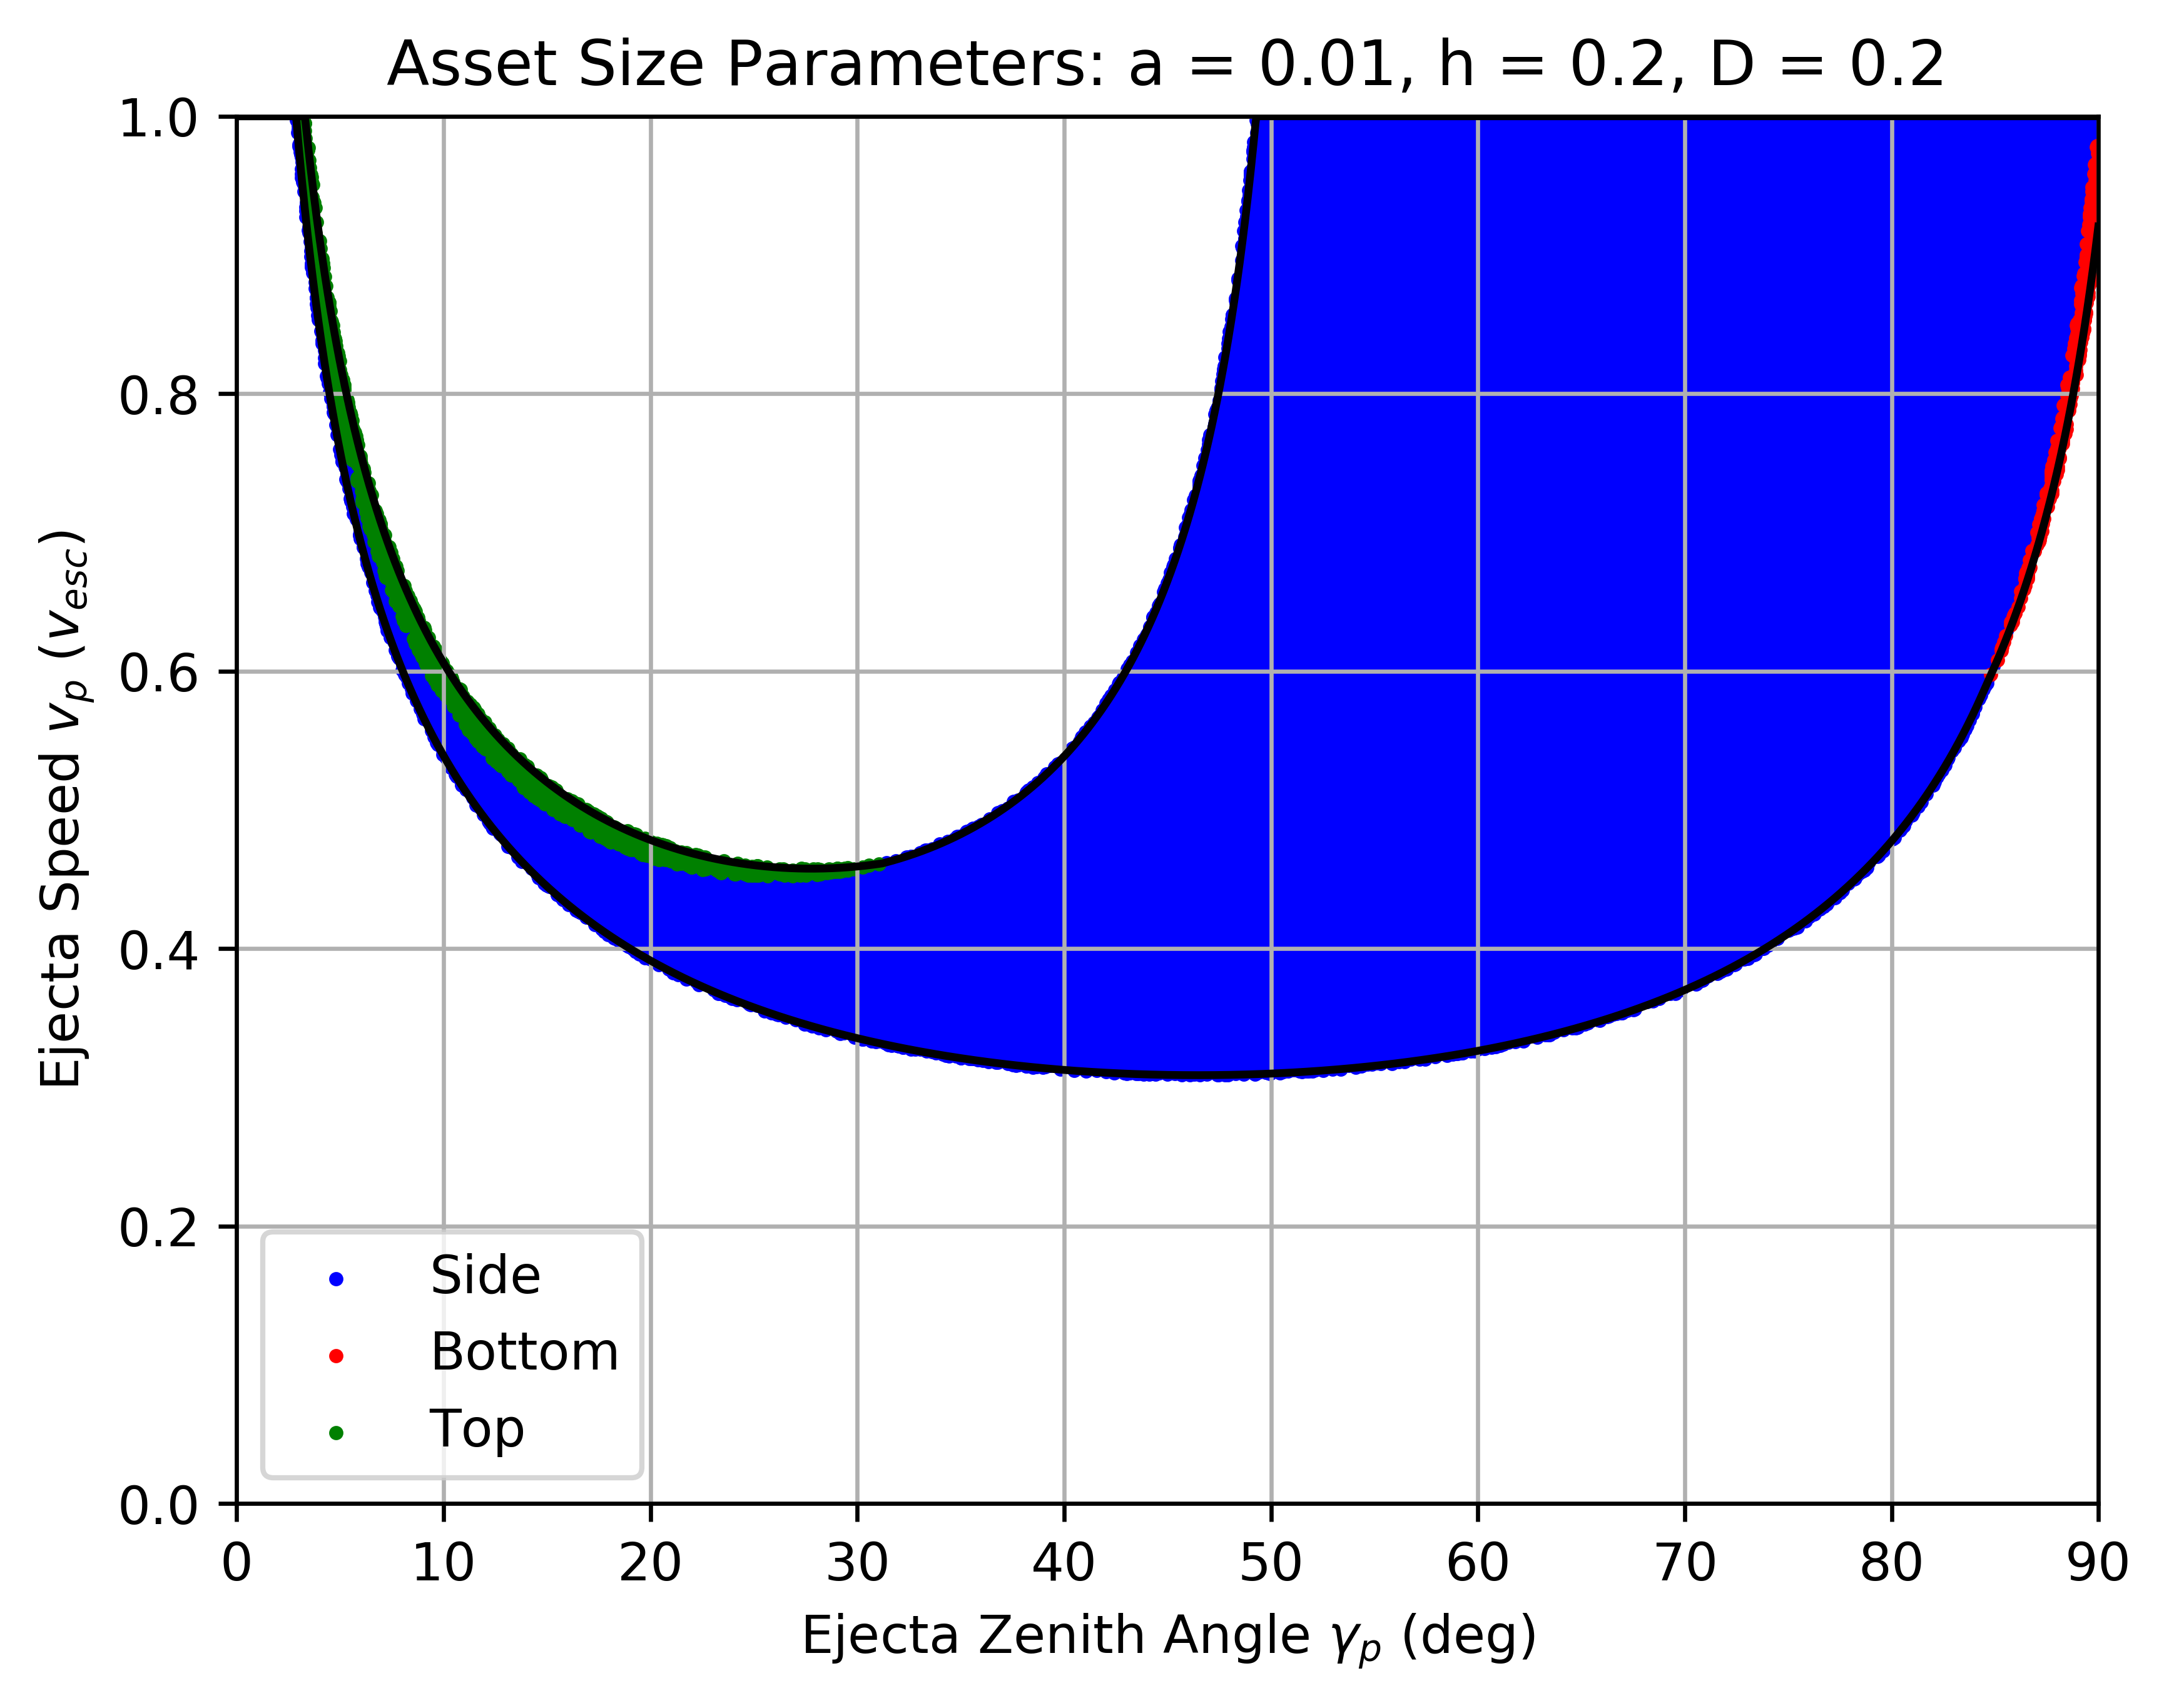
\includegraphics[width=.98\linewidth]{asset_speed_zenith_plot_1.010e+00_1.000e-02_2.000e-01_2.000e-01.png}  
		%\caption{Put your sub-caption here}
		\label{fig:sub-asset_speed_zenith_h1_7}
	\end{subfigure}
	\begin{subfigure}[t]{.32\textwidth}
		\centering
		% include fourth image
		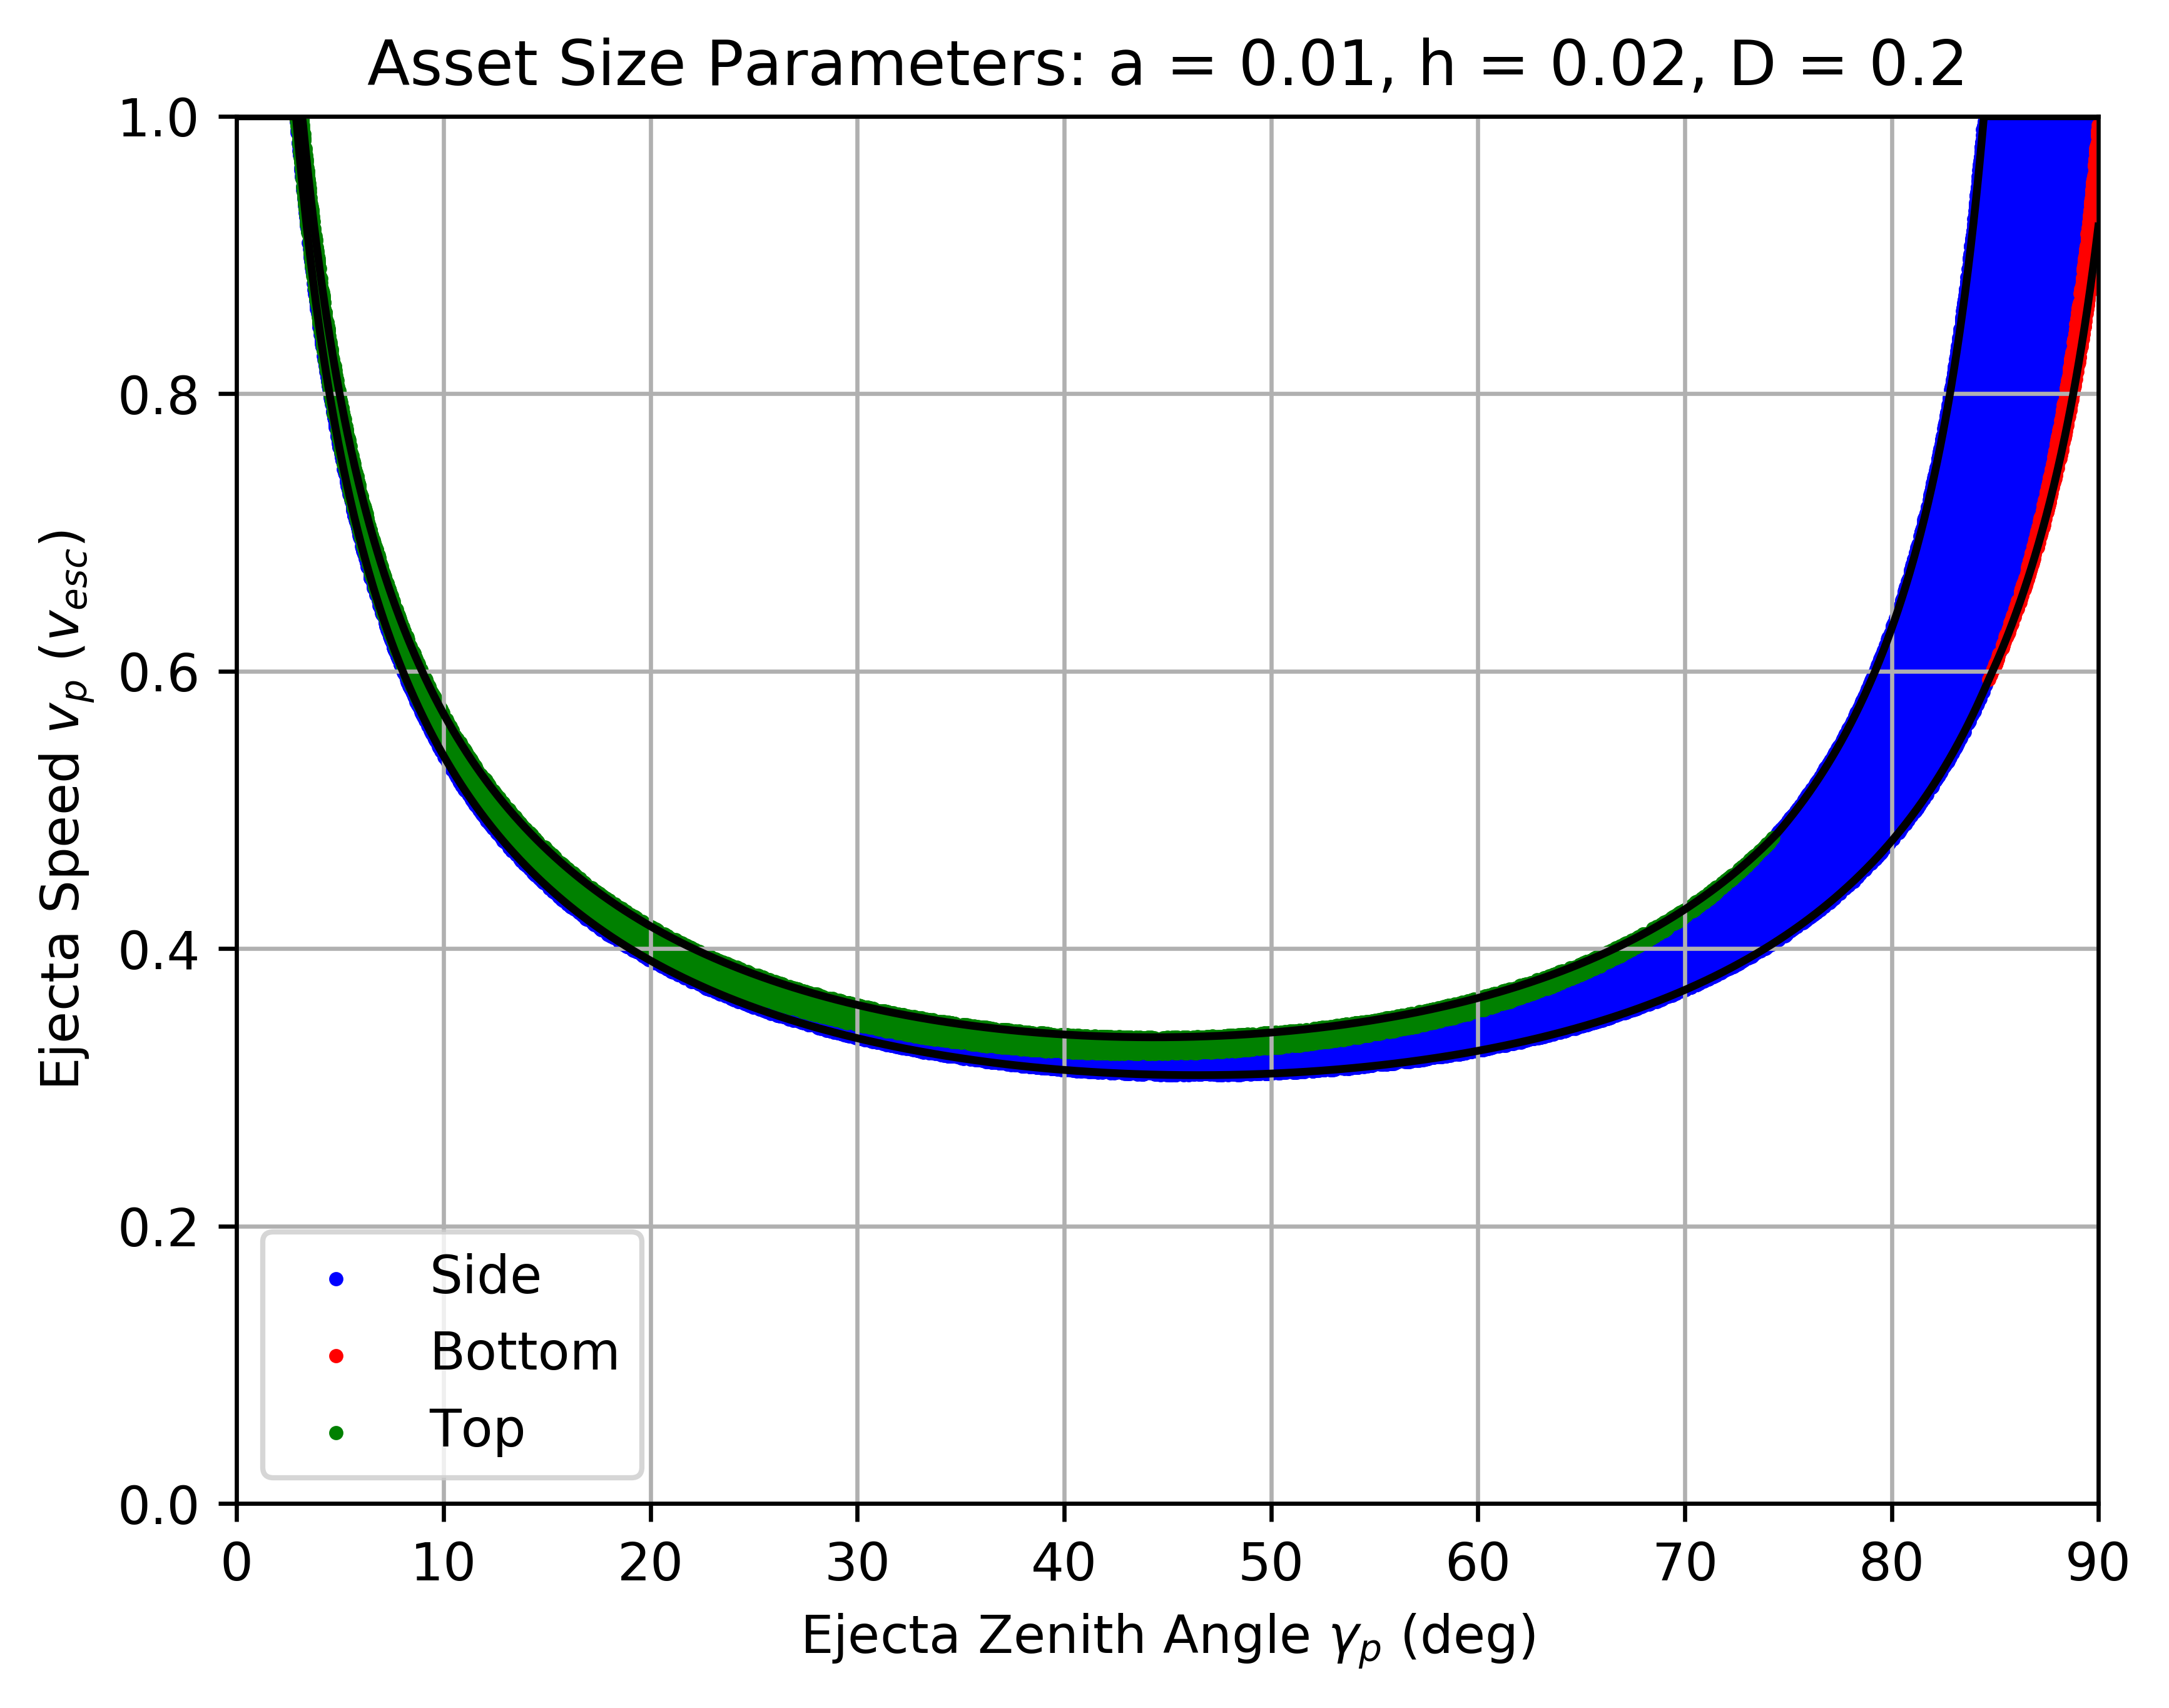
\includegraphics[width=.98\linewidth]{asset_speed_zenith_plot_1.010e+00_1.000e-02_2.000e-02_2.000e-01.png}  
		%\caption{Put your sub-caption here}
		\label{fig:sub-asset_speed_zenith_h1_8}
	\end{subfigure}
	\begin{subfigure}[t]{.32\textwidth}
		\centering
		% include fourth image
		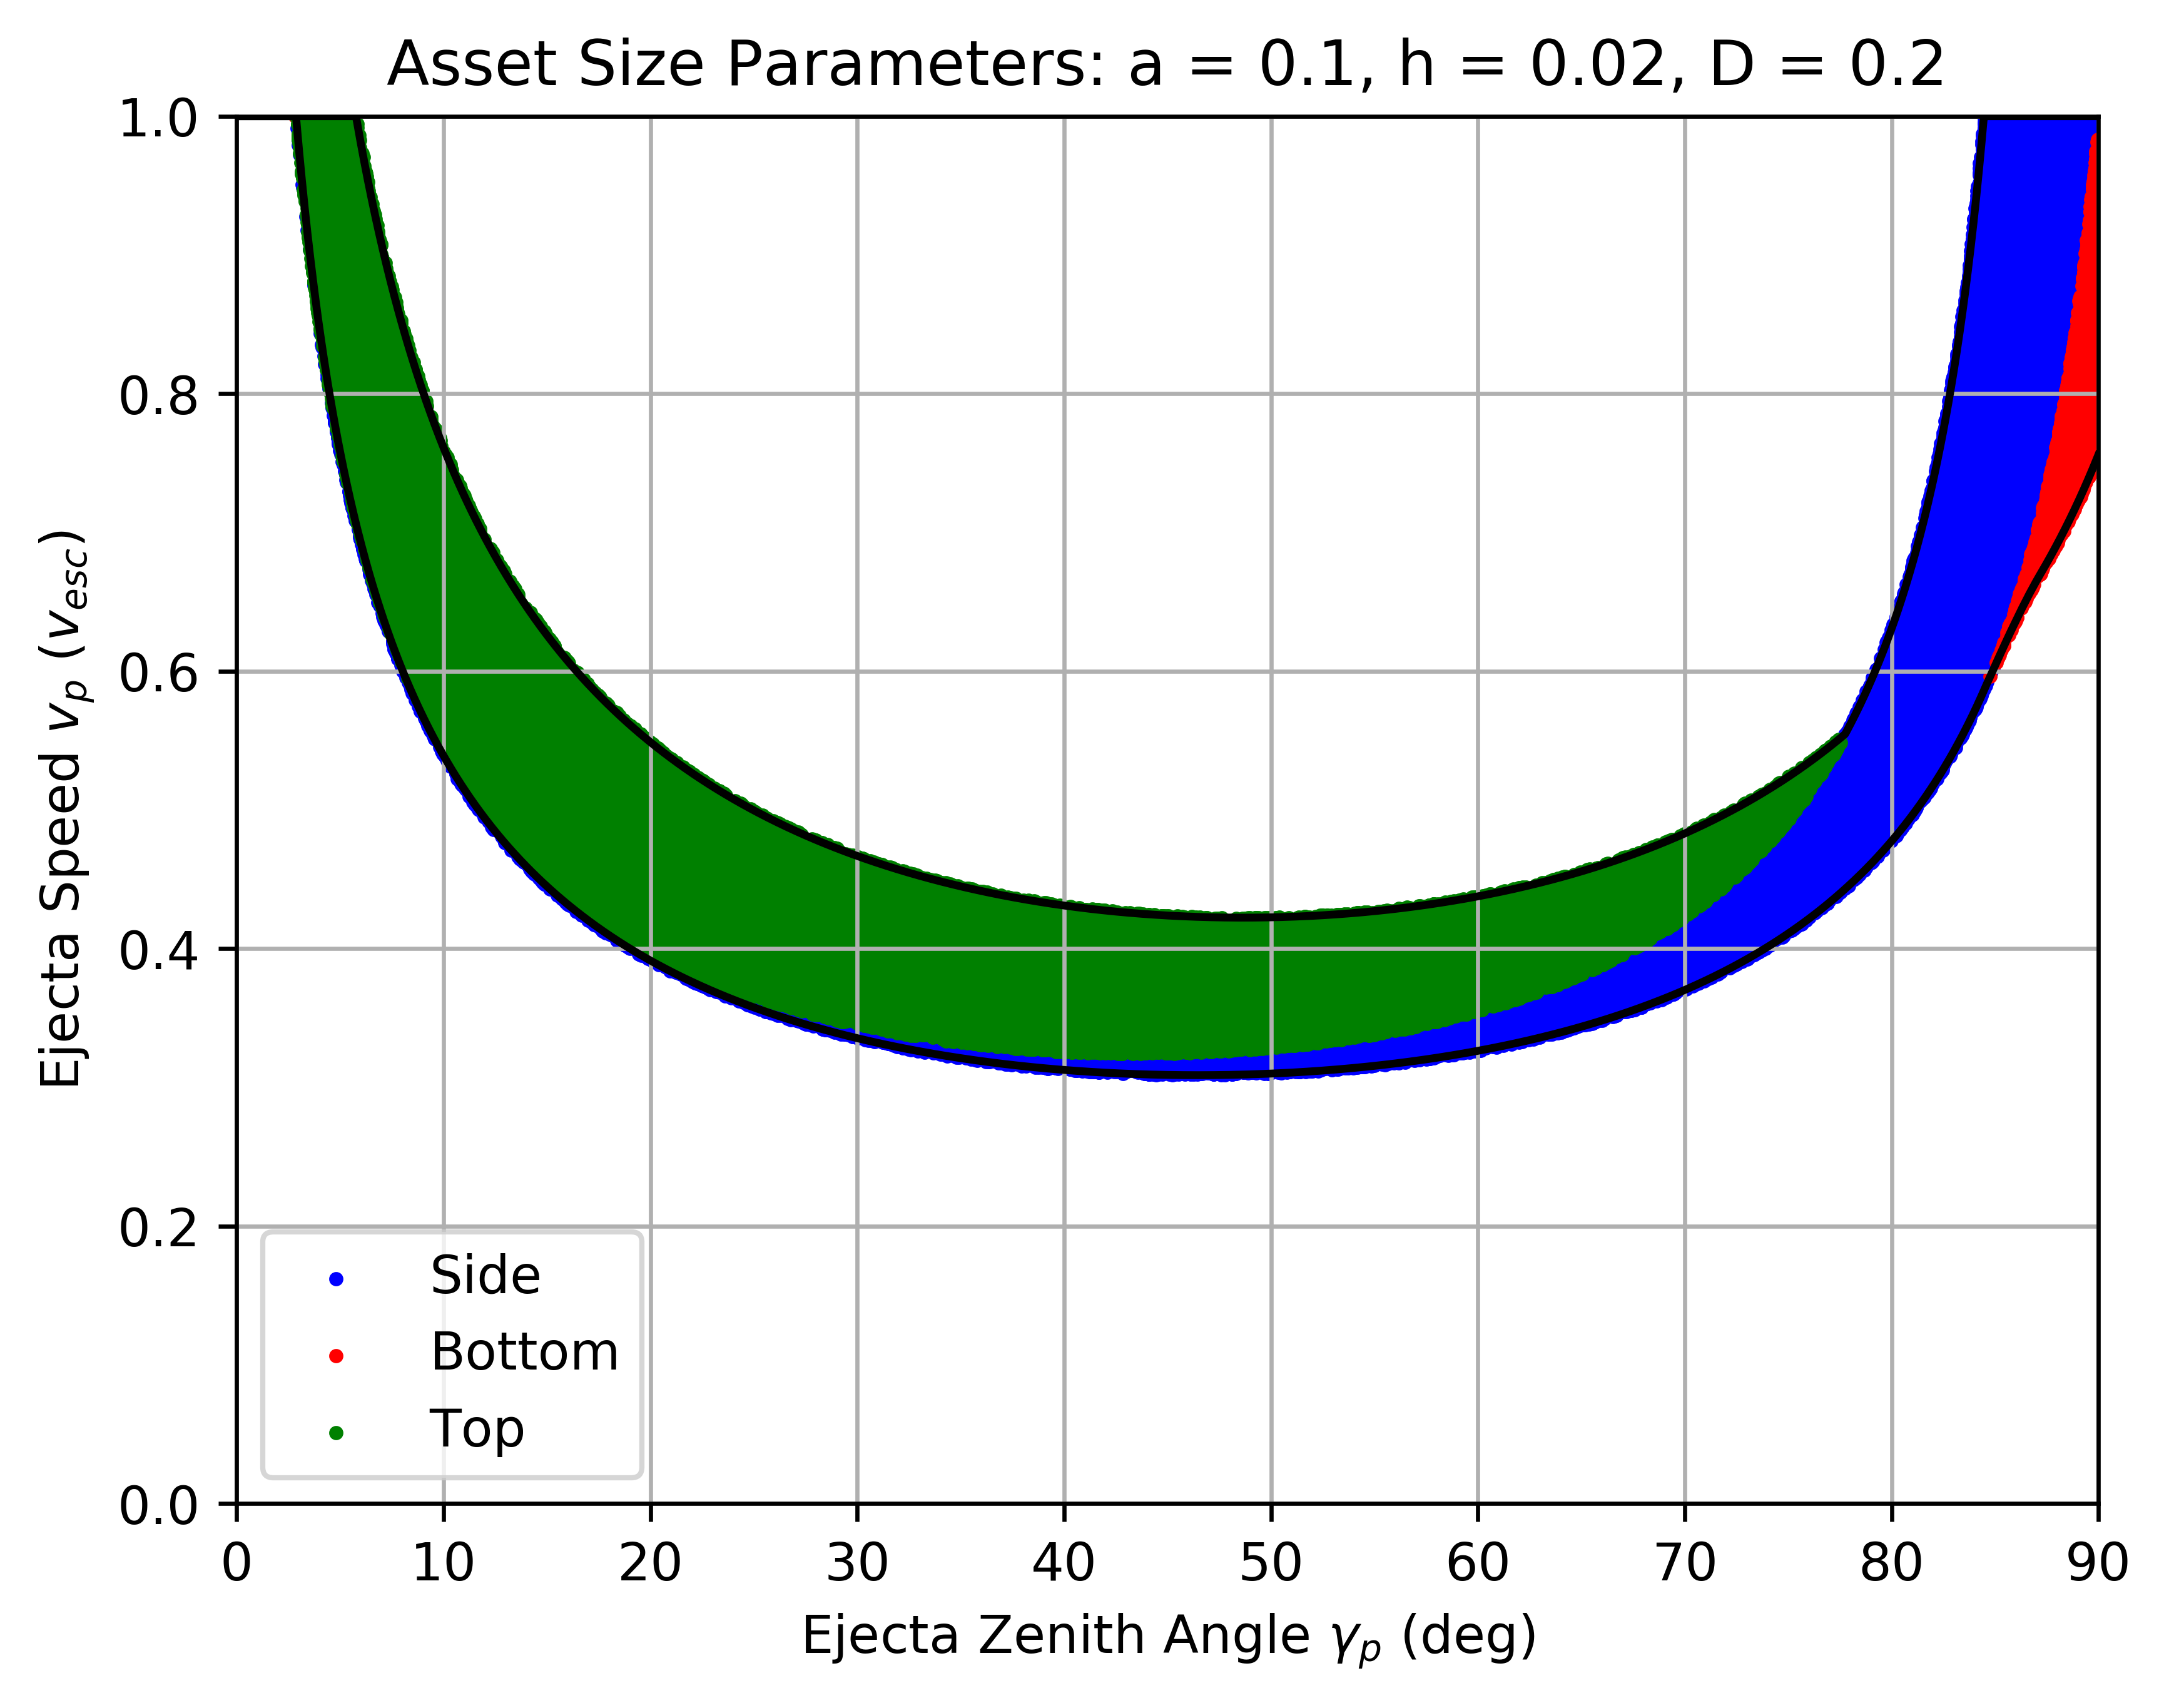
\includegraphics[width=.98\linewidth]{asset_speed_zenith_plot_1.010e+00_1.000e-01_2.000e-02_2.000e-01.png}  
		%\caption{Put your sub-caption here}
		\label{fig:sub-asset_speed_zenith_h1_9}
	\end{subfigure}
	
	\begin{subfigure}[t]{.32\textwidth}
		\centering
		% include third image
		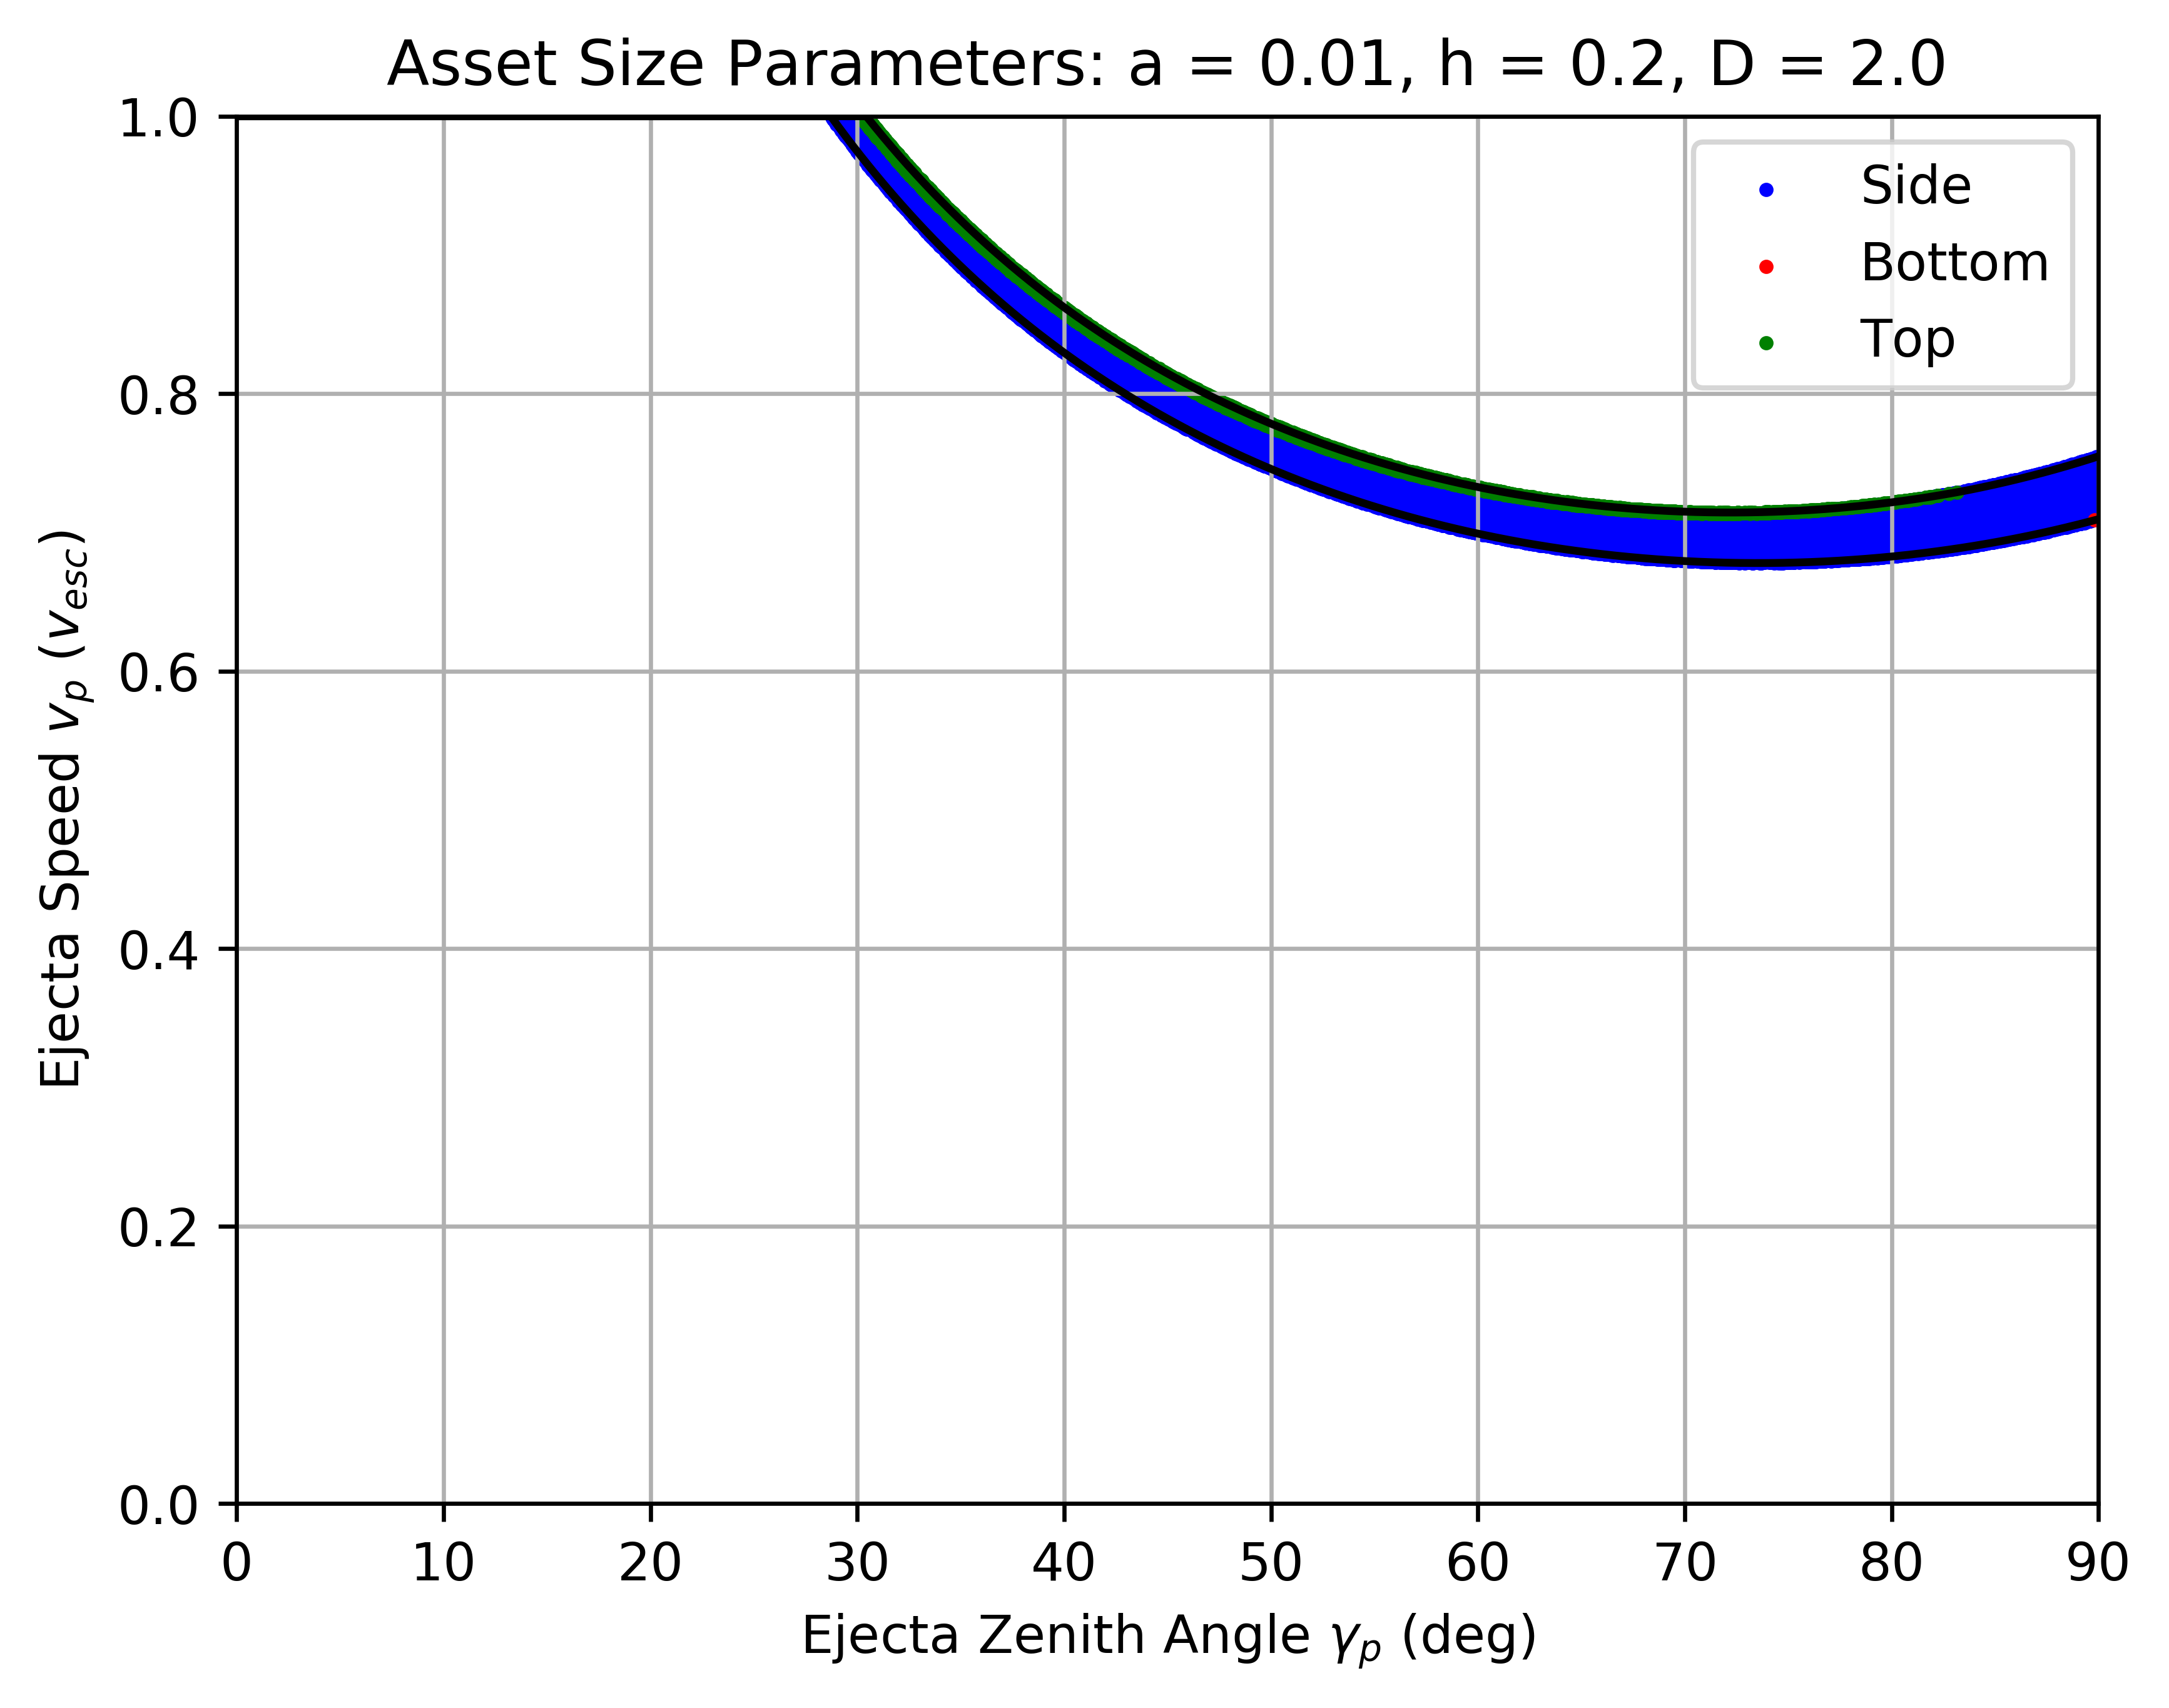
\includegraphics[width=.98\linewidth]{asset_speed_zenith_plot_1.010e+00_1.000e-02_2.000e-01_2.000e+00.png}  
		%\caption{Put your sub-caption here}
		\label{fig:sub-asset_speed_zenith_h1_10}
	\end{subfigure}
	\begin{subfigure}[t]{.32\textwidth}
		\centering
		% include fourth image
		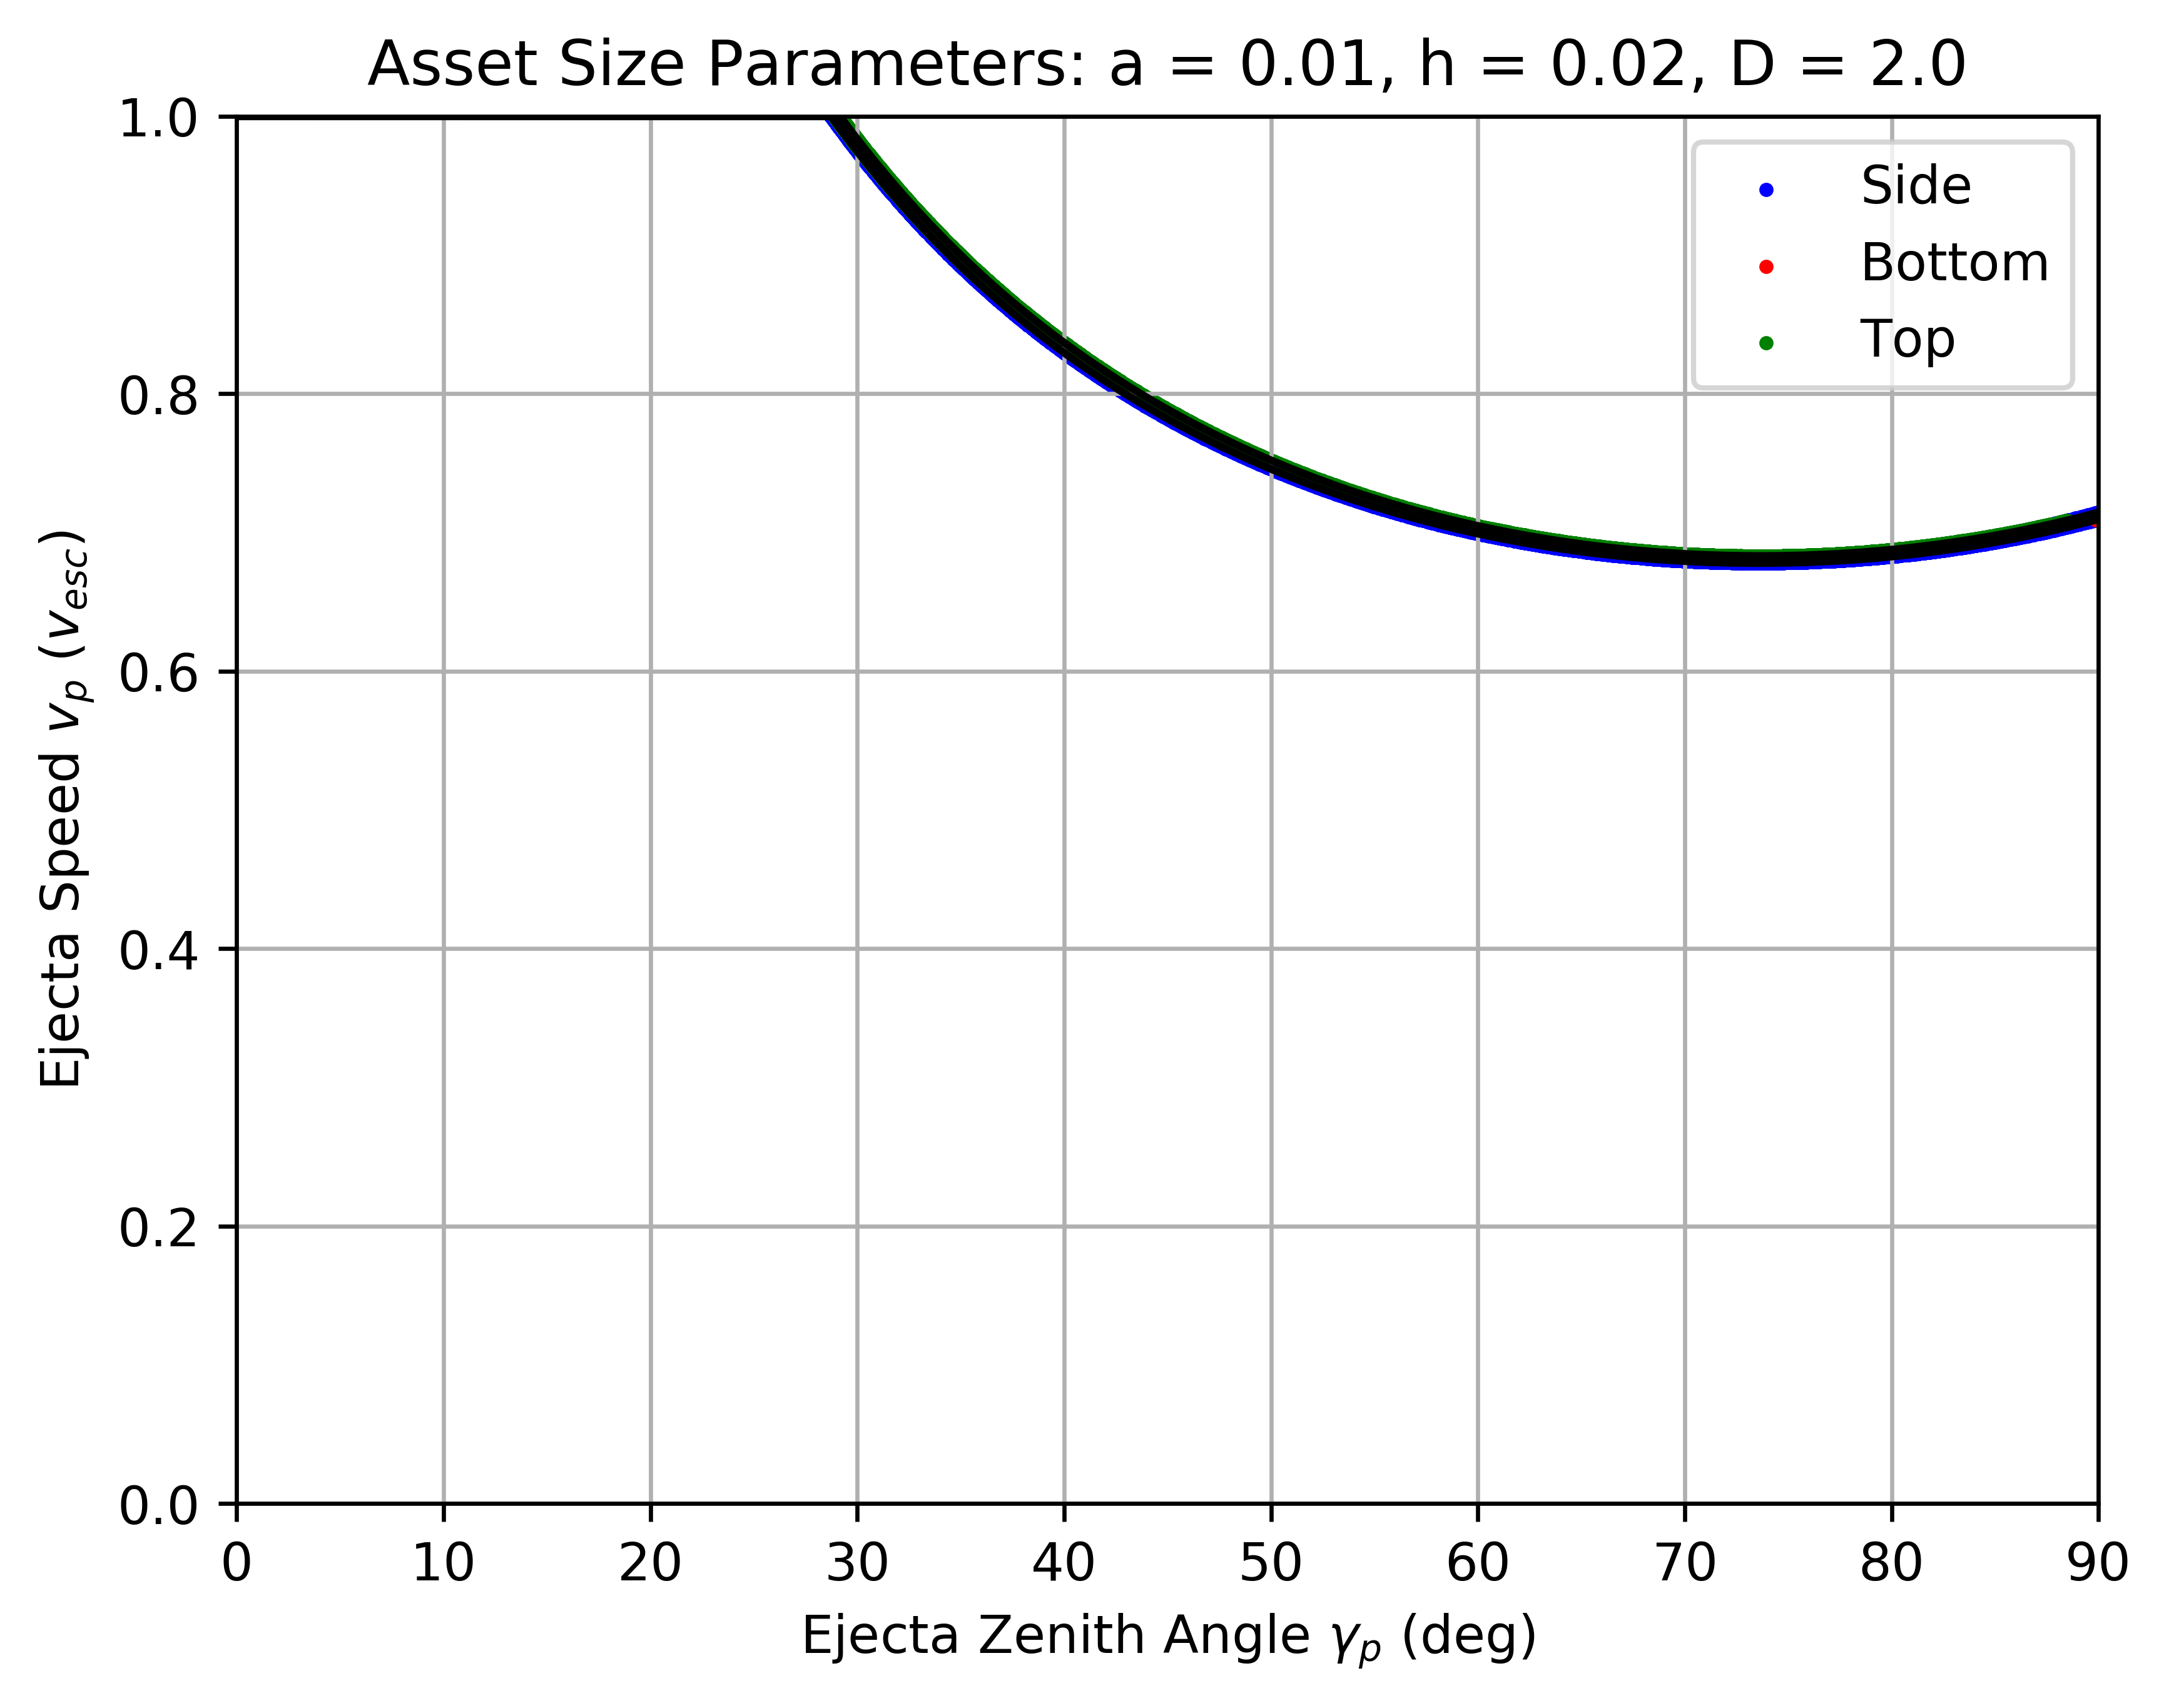
\includegraphics[width=.98\linewidth]{asset_speed_zenith_plot_1.010e+00_1.000e-02_2.000e-02_2.000e+00.png}  
		%\caption{Put your sub-caption here}
		\label{fig:sub-asset_speed_zenith_h1_11}
	\end{subfigure}
	\begin{subfigure}[t]{.32\textwidth}
		\centering
		% include fourth image
		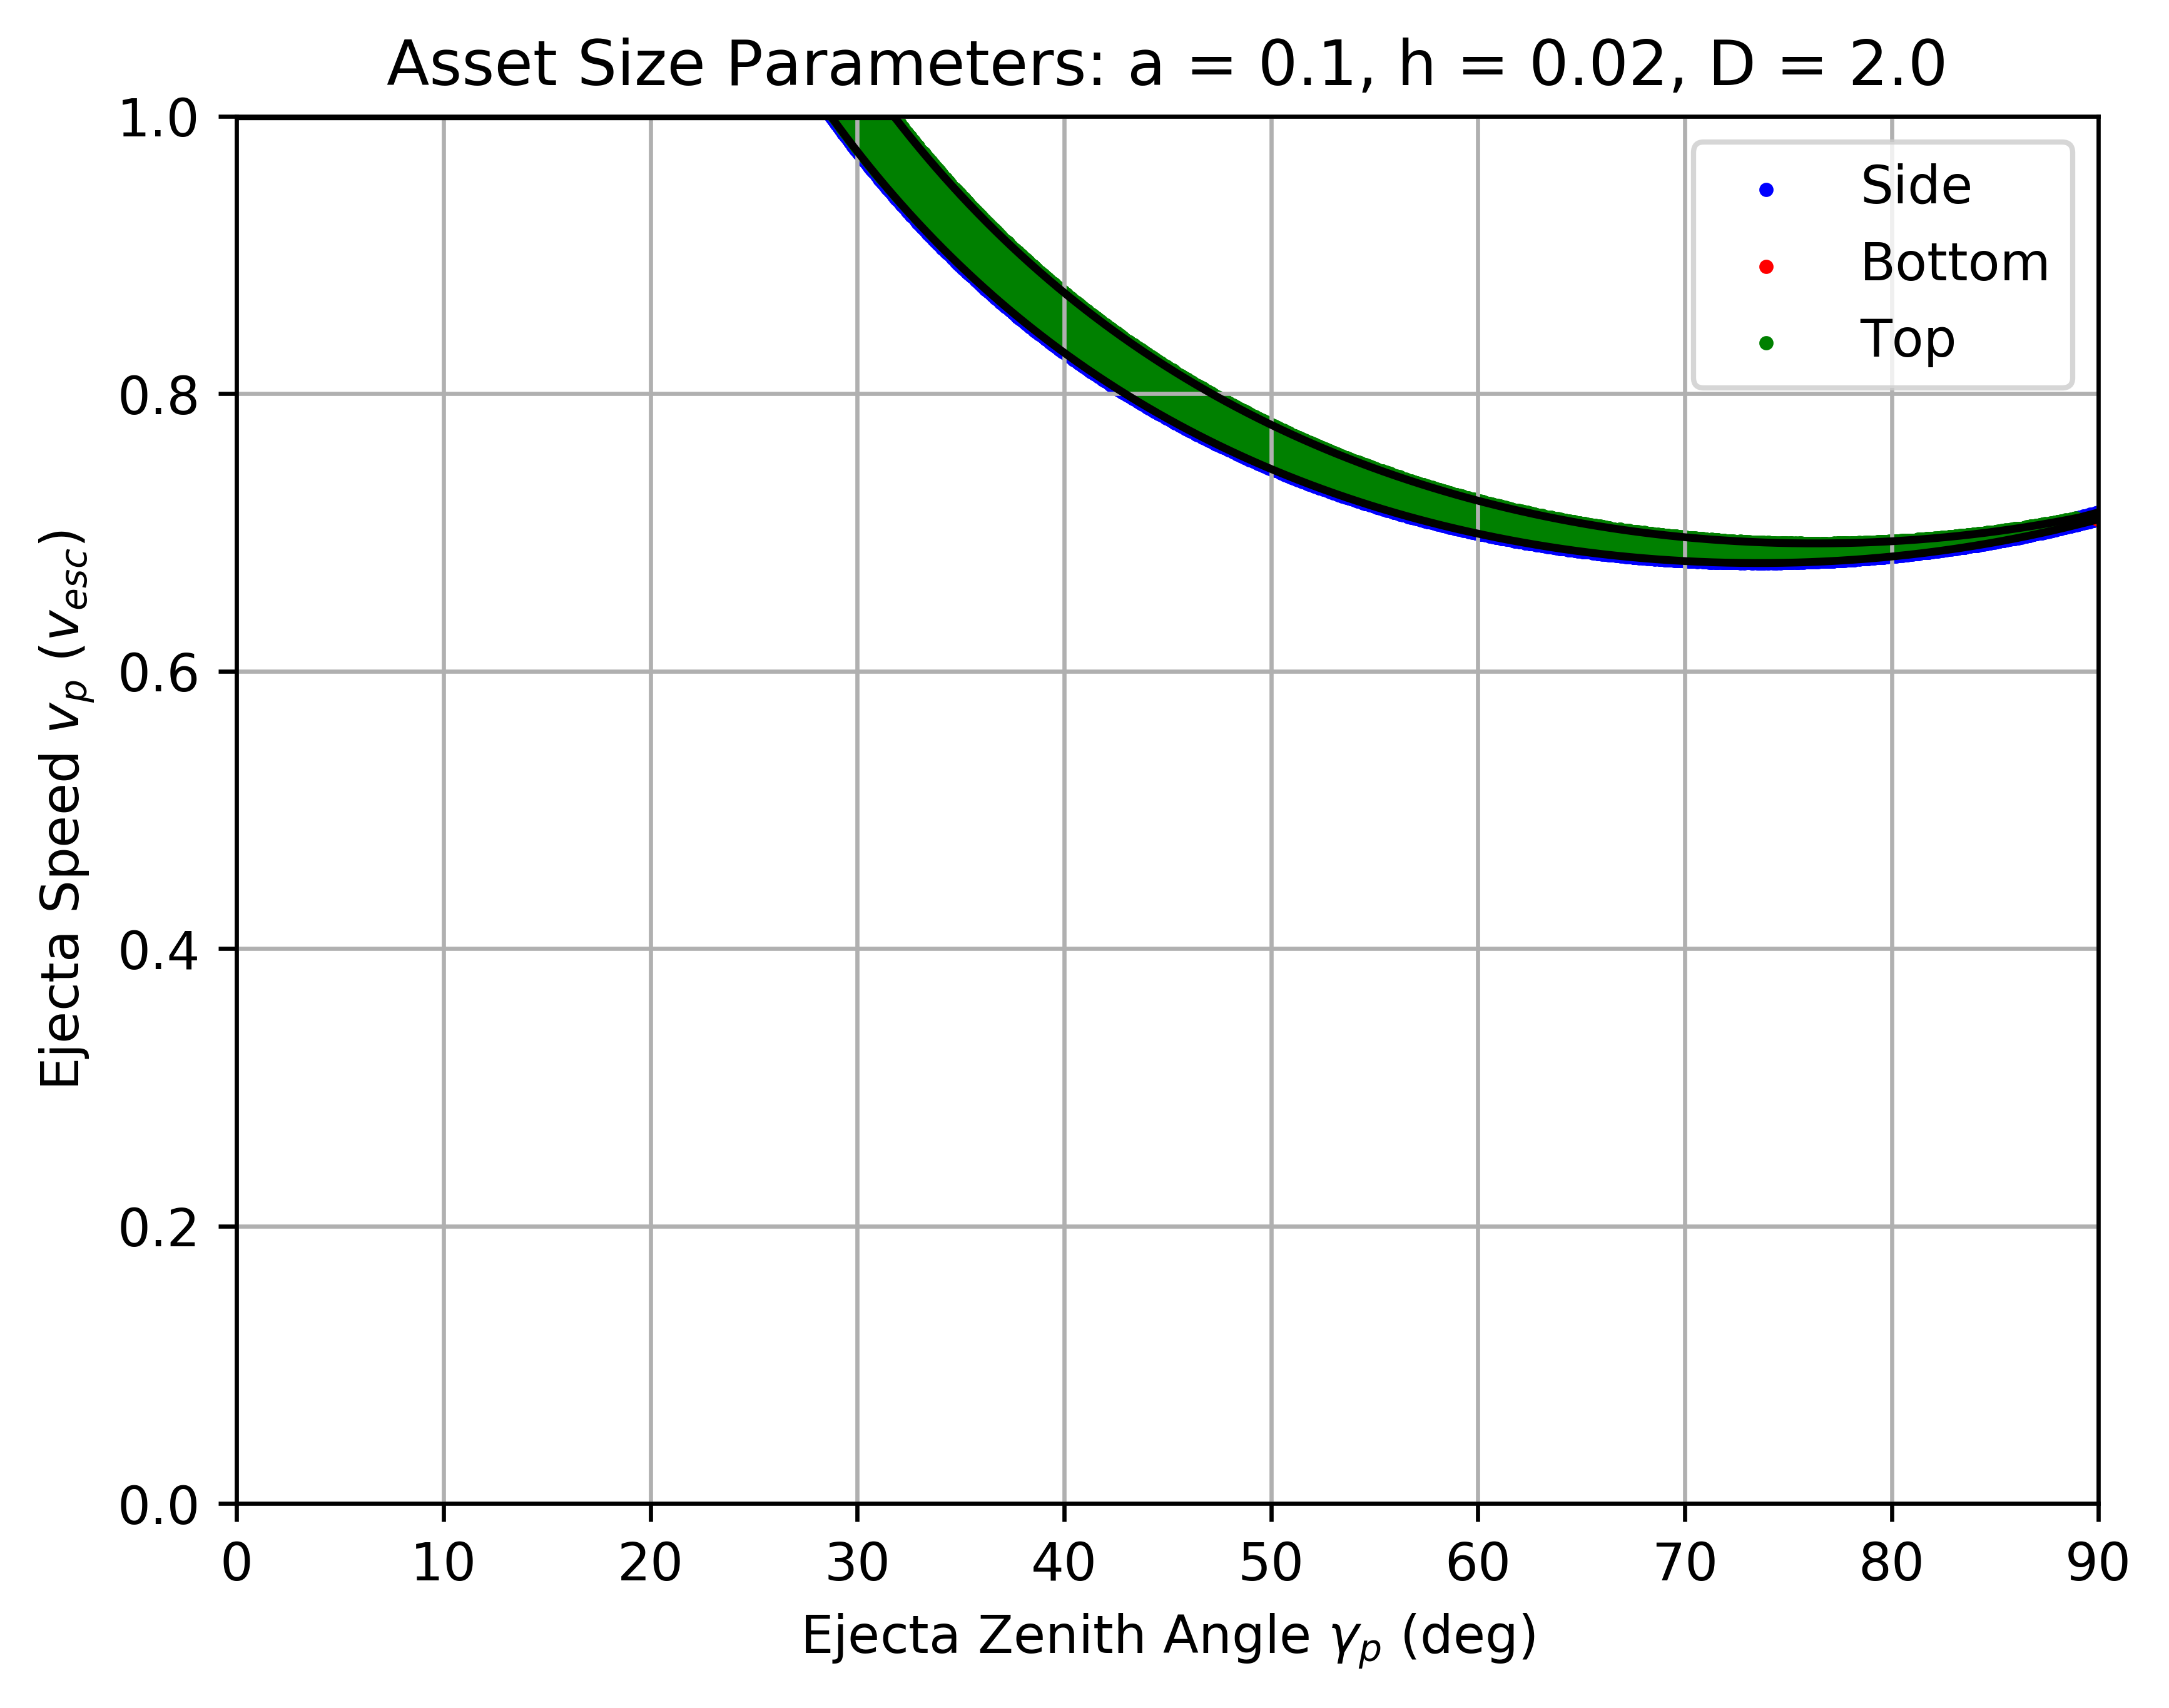
\includegraphics[width=.98\linewidth]{asset_speed_zenith_plot_1.010e+00_1.000e-01_2.000e-02_2.000e+00.png}  
		%\caption{Put your sub-caption here}
		\label{fig:sub-asset_speed_zenith_h1_12}
	\end{subfigure}
	
	\caption{A matrix of plots showing the ejecta hitting a cylindrical asset (in a plane intersecting the cylinder's symmetry axis) with a height above the surface of $0.01 r_m$ for various asset sizes and crater-to-asset distances. Each plot gives three colors for the ejecta hitting the side (blue), bottom (red), and the top (green) as a function of initial ejecta speed $v_p$ vs.\ initial ejecta zenith angle $\gamma_p$.}
	\label{fig:asset_speed_zenith_comparison_h1}
\end{figure}








\begin{figure}
	\begin{subfigure}[t]{.32\textwidth}
		\centering
		% include first image
		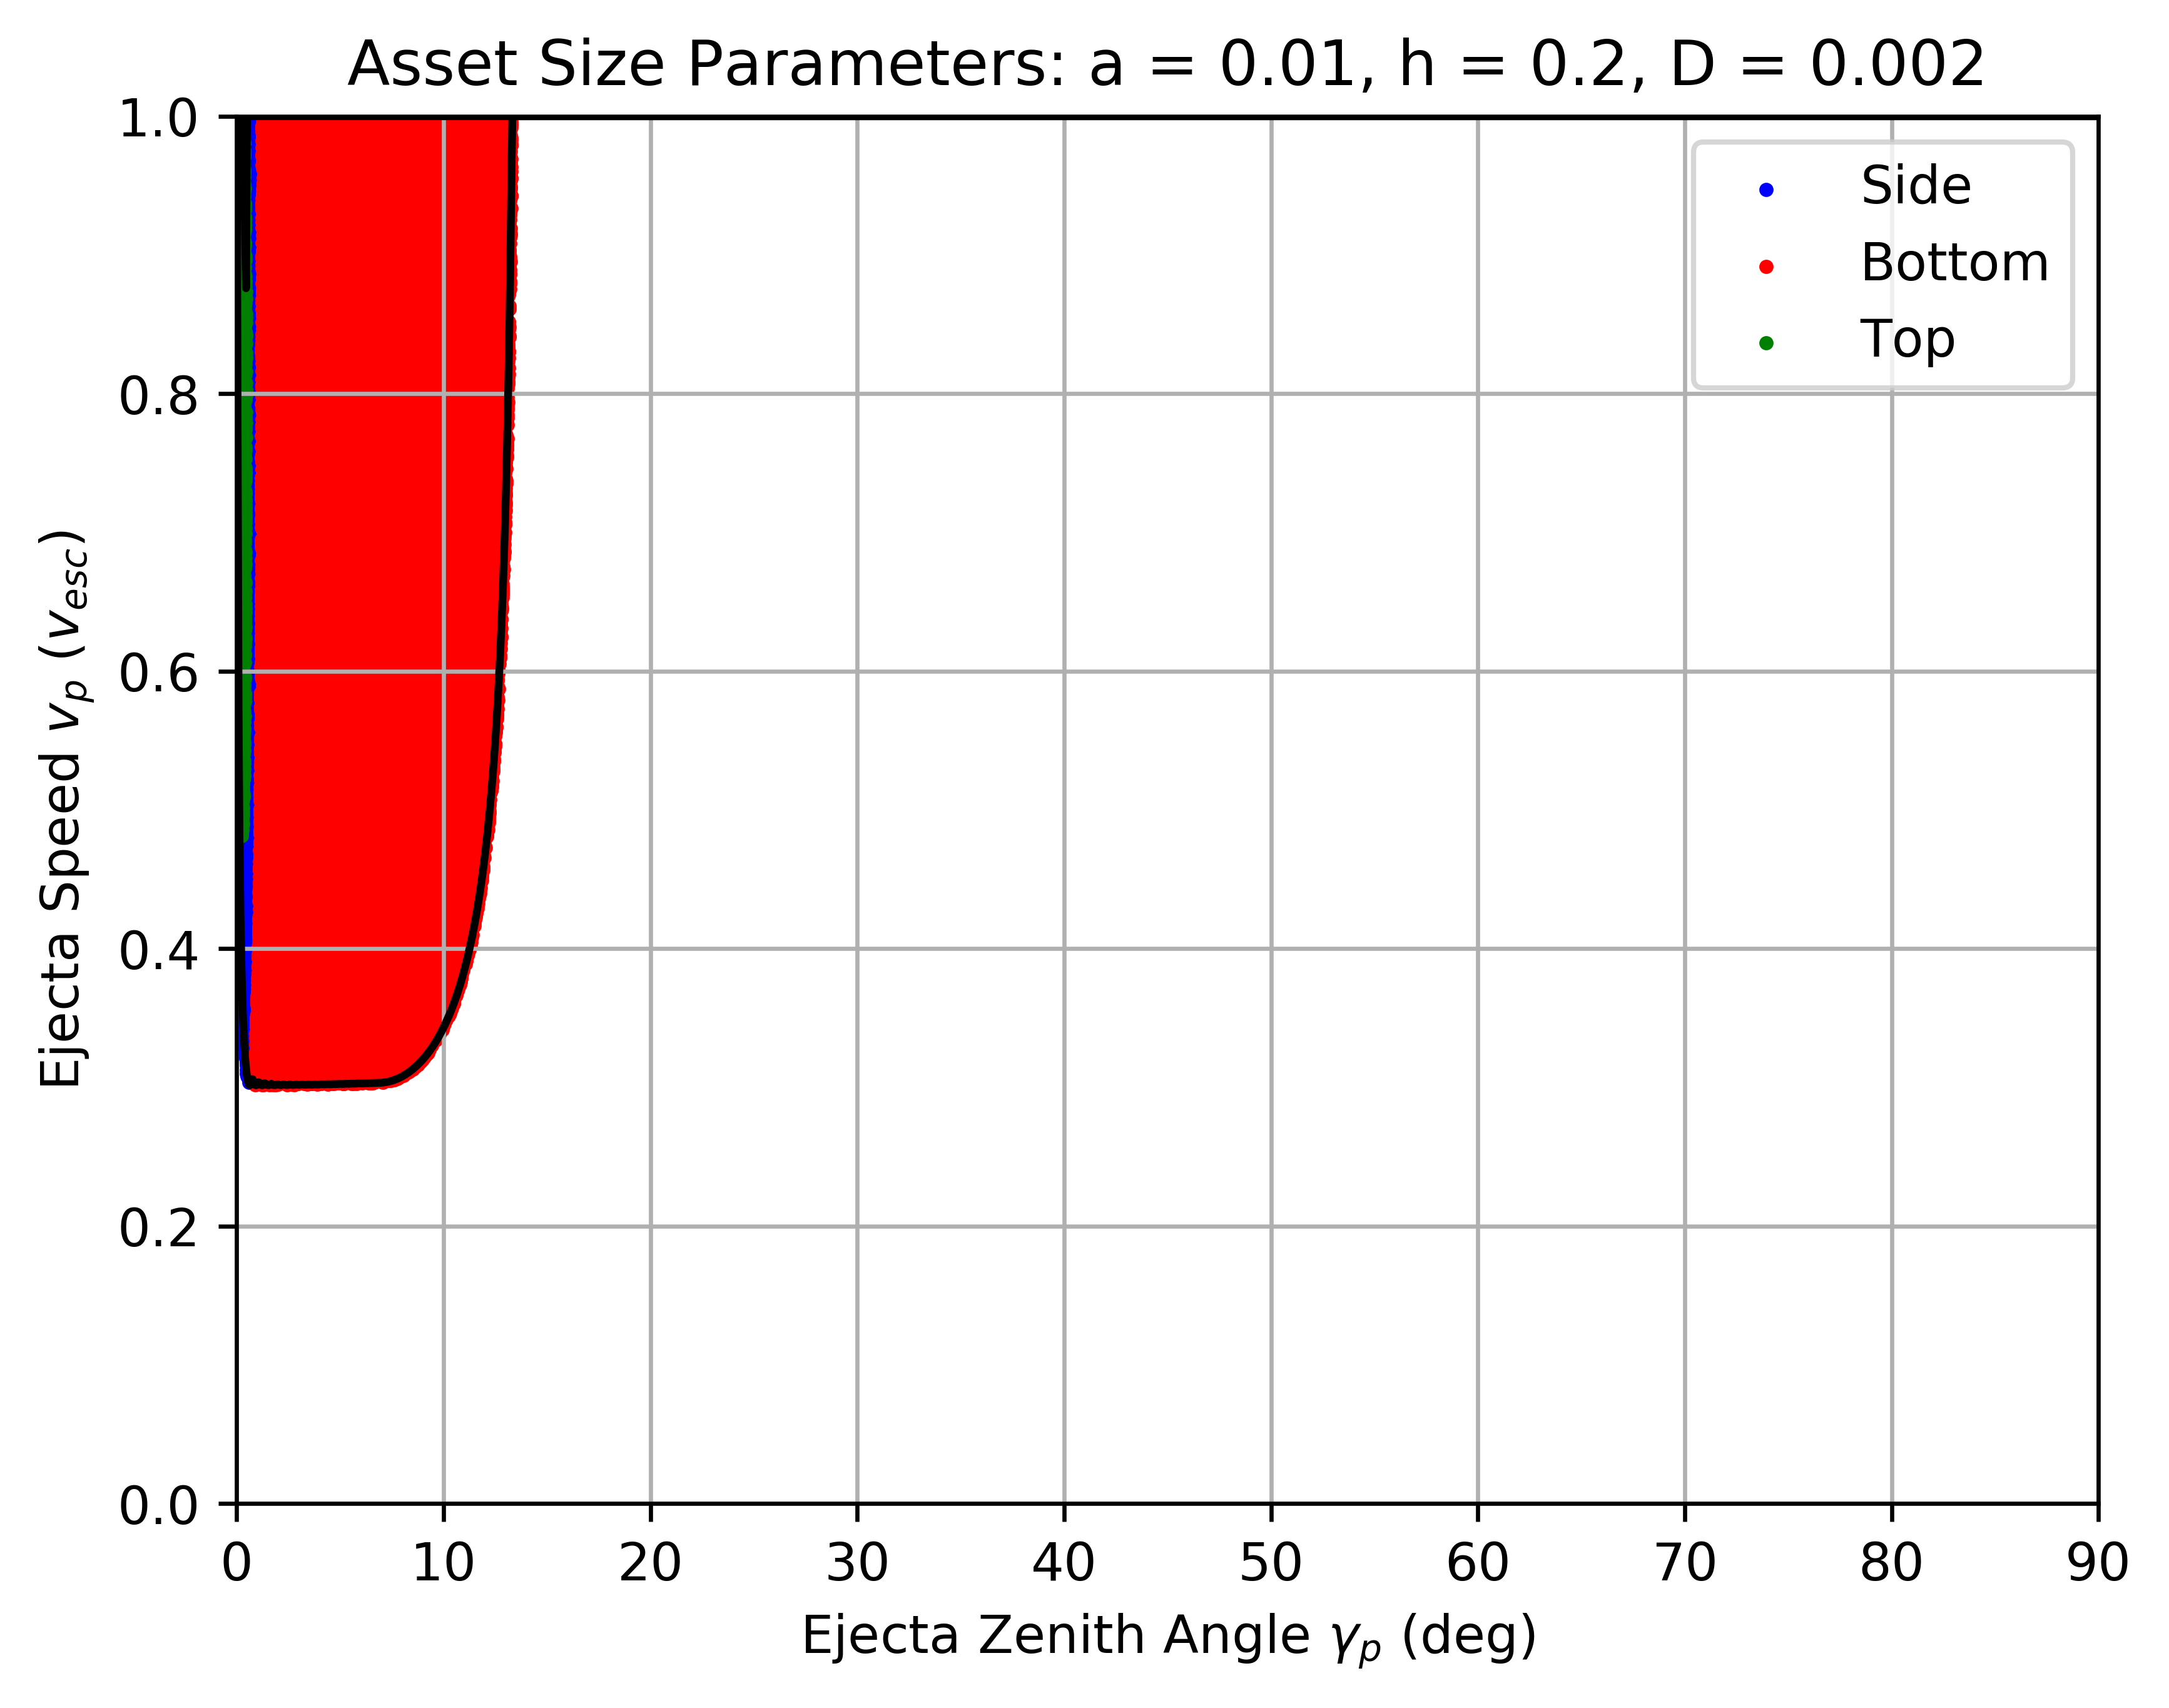
\includegraphics[width=.98\linewidth]{asset_speed_zenith_plot_1.100e+00_1.000e-02_2.000e-01_2.000e-03.png}  
		%\caption{Put your sub-caption here}
		\label{fig:sub-asset_speed_zenith_h2_1}
	\end{subfigure}
	\begin{subfigure}[t]{.32\textwidth}
		\centering
		% include second image
		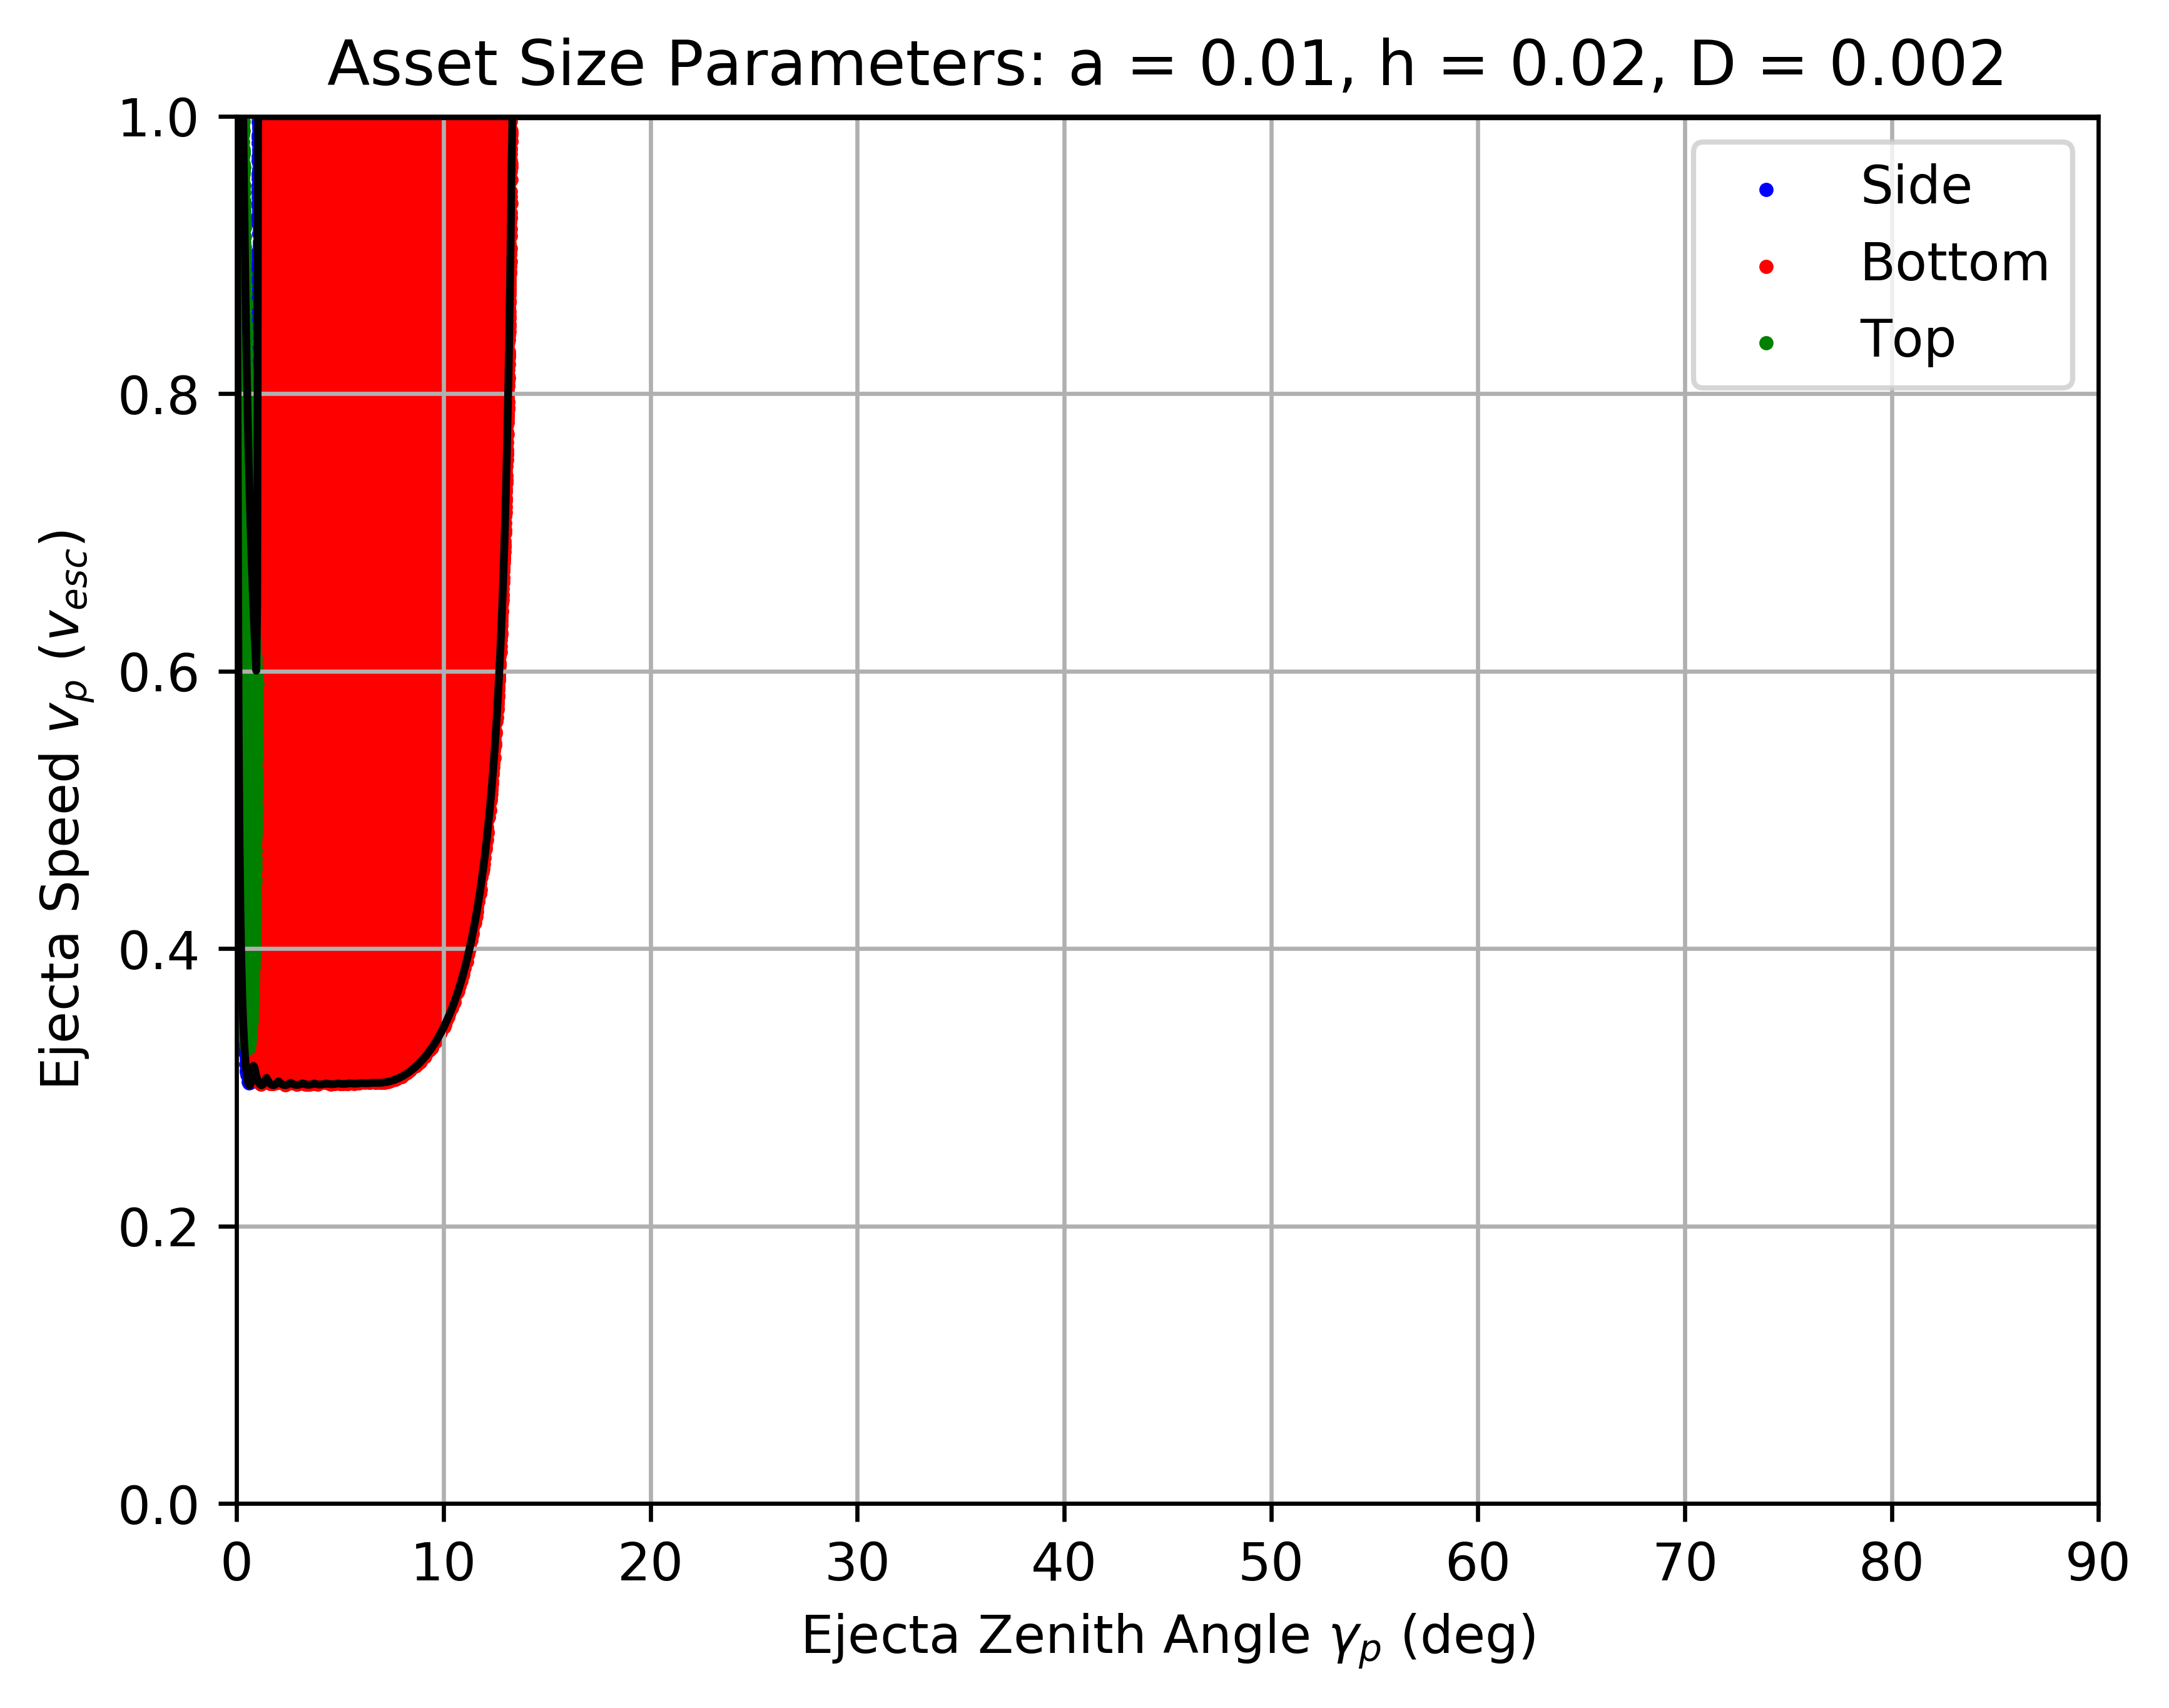
\includegraphics[width=.98\linewidth]{asset_speed_zenith_plot_1.100e+00_1.000e-02_2.000e-02_2.000e-03.png}  
		%\caption{Put your sub-caption here}
		\label{fig:sub-asset_speed_zenith_h2_2}
	\end{subfigure}
	\begin{subfigure}[t]{.32\textwidth}
		\centering
		% include second image
		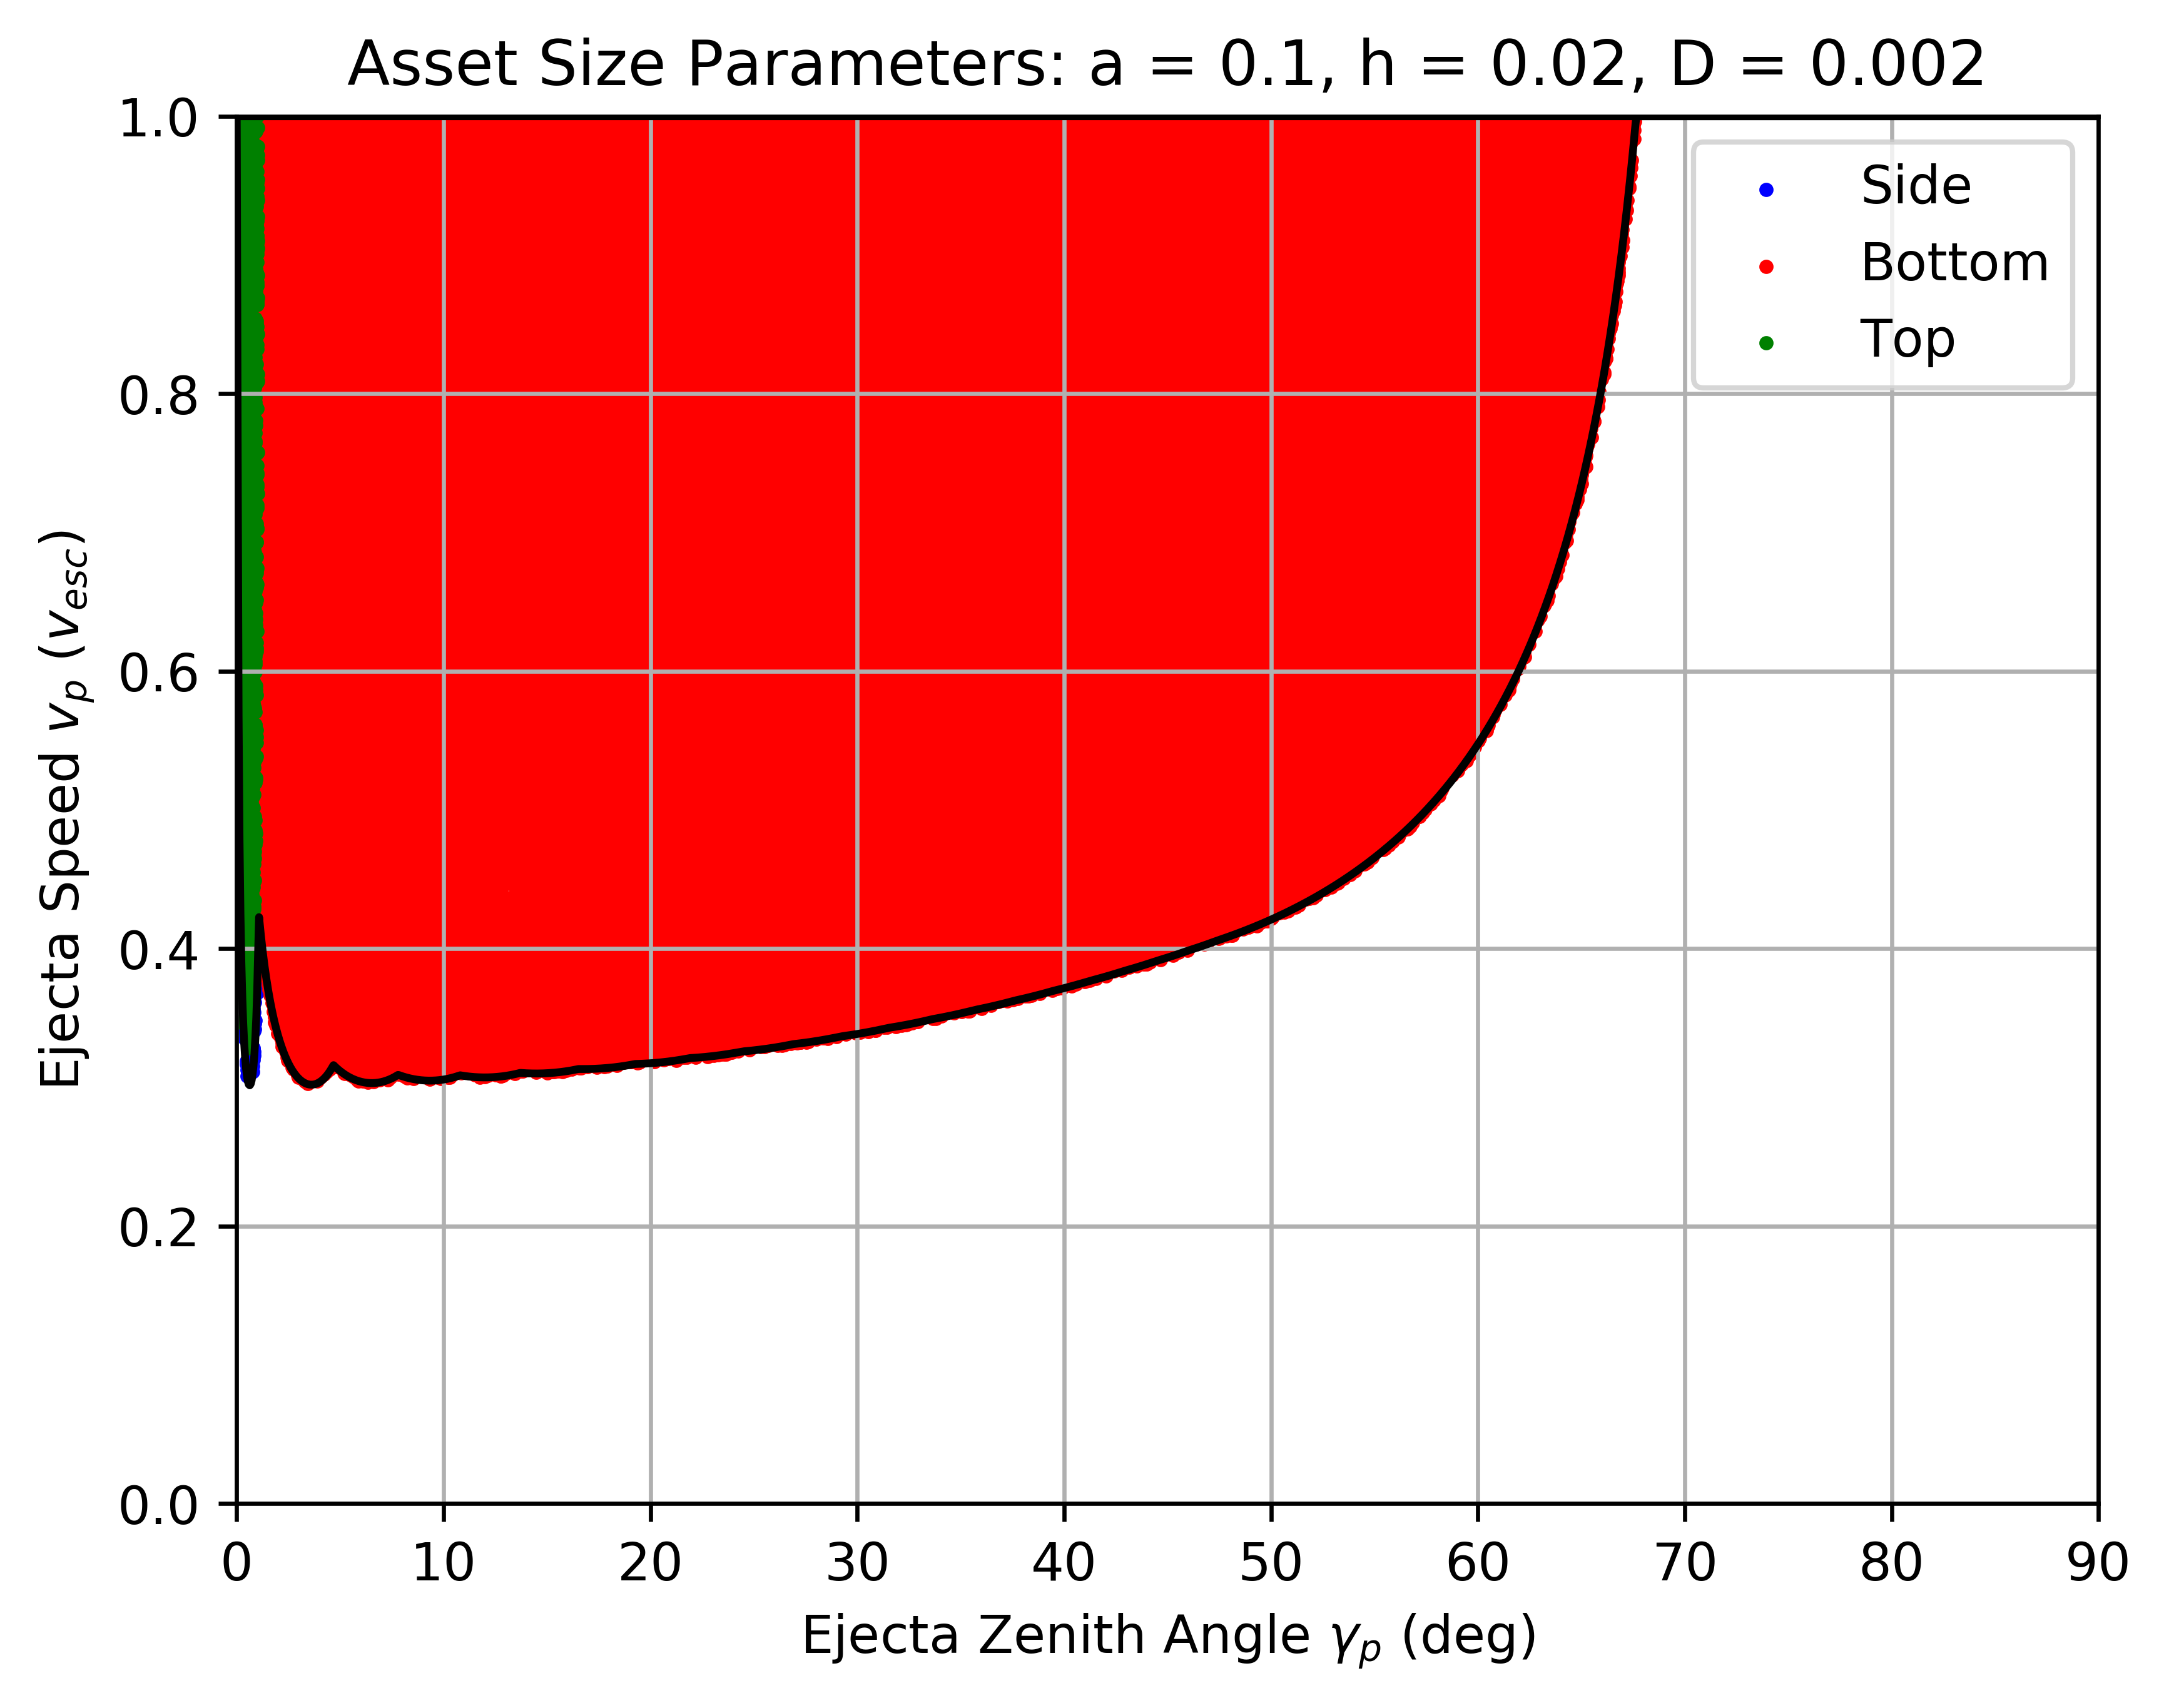
\includegraphics[width=.98\linewidth]{asset_speed_zenith_plot_1.100e+00_1.000e-01_2.000e-02_2.000e-03.png}  
		%\caption{Put your sub-caption here}
		\label{fig:sub-asset_speed_zenith_h2_3}
	\end{subfigure}
	
	%\newline
	
	\begin{subfigure}[t]{.32\textwidth}
		\centering
		% include third image
		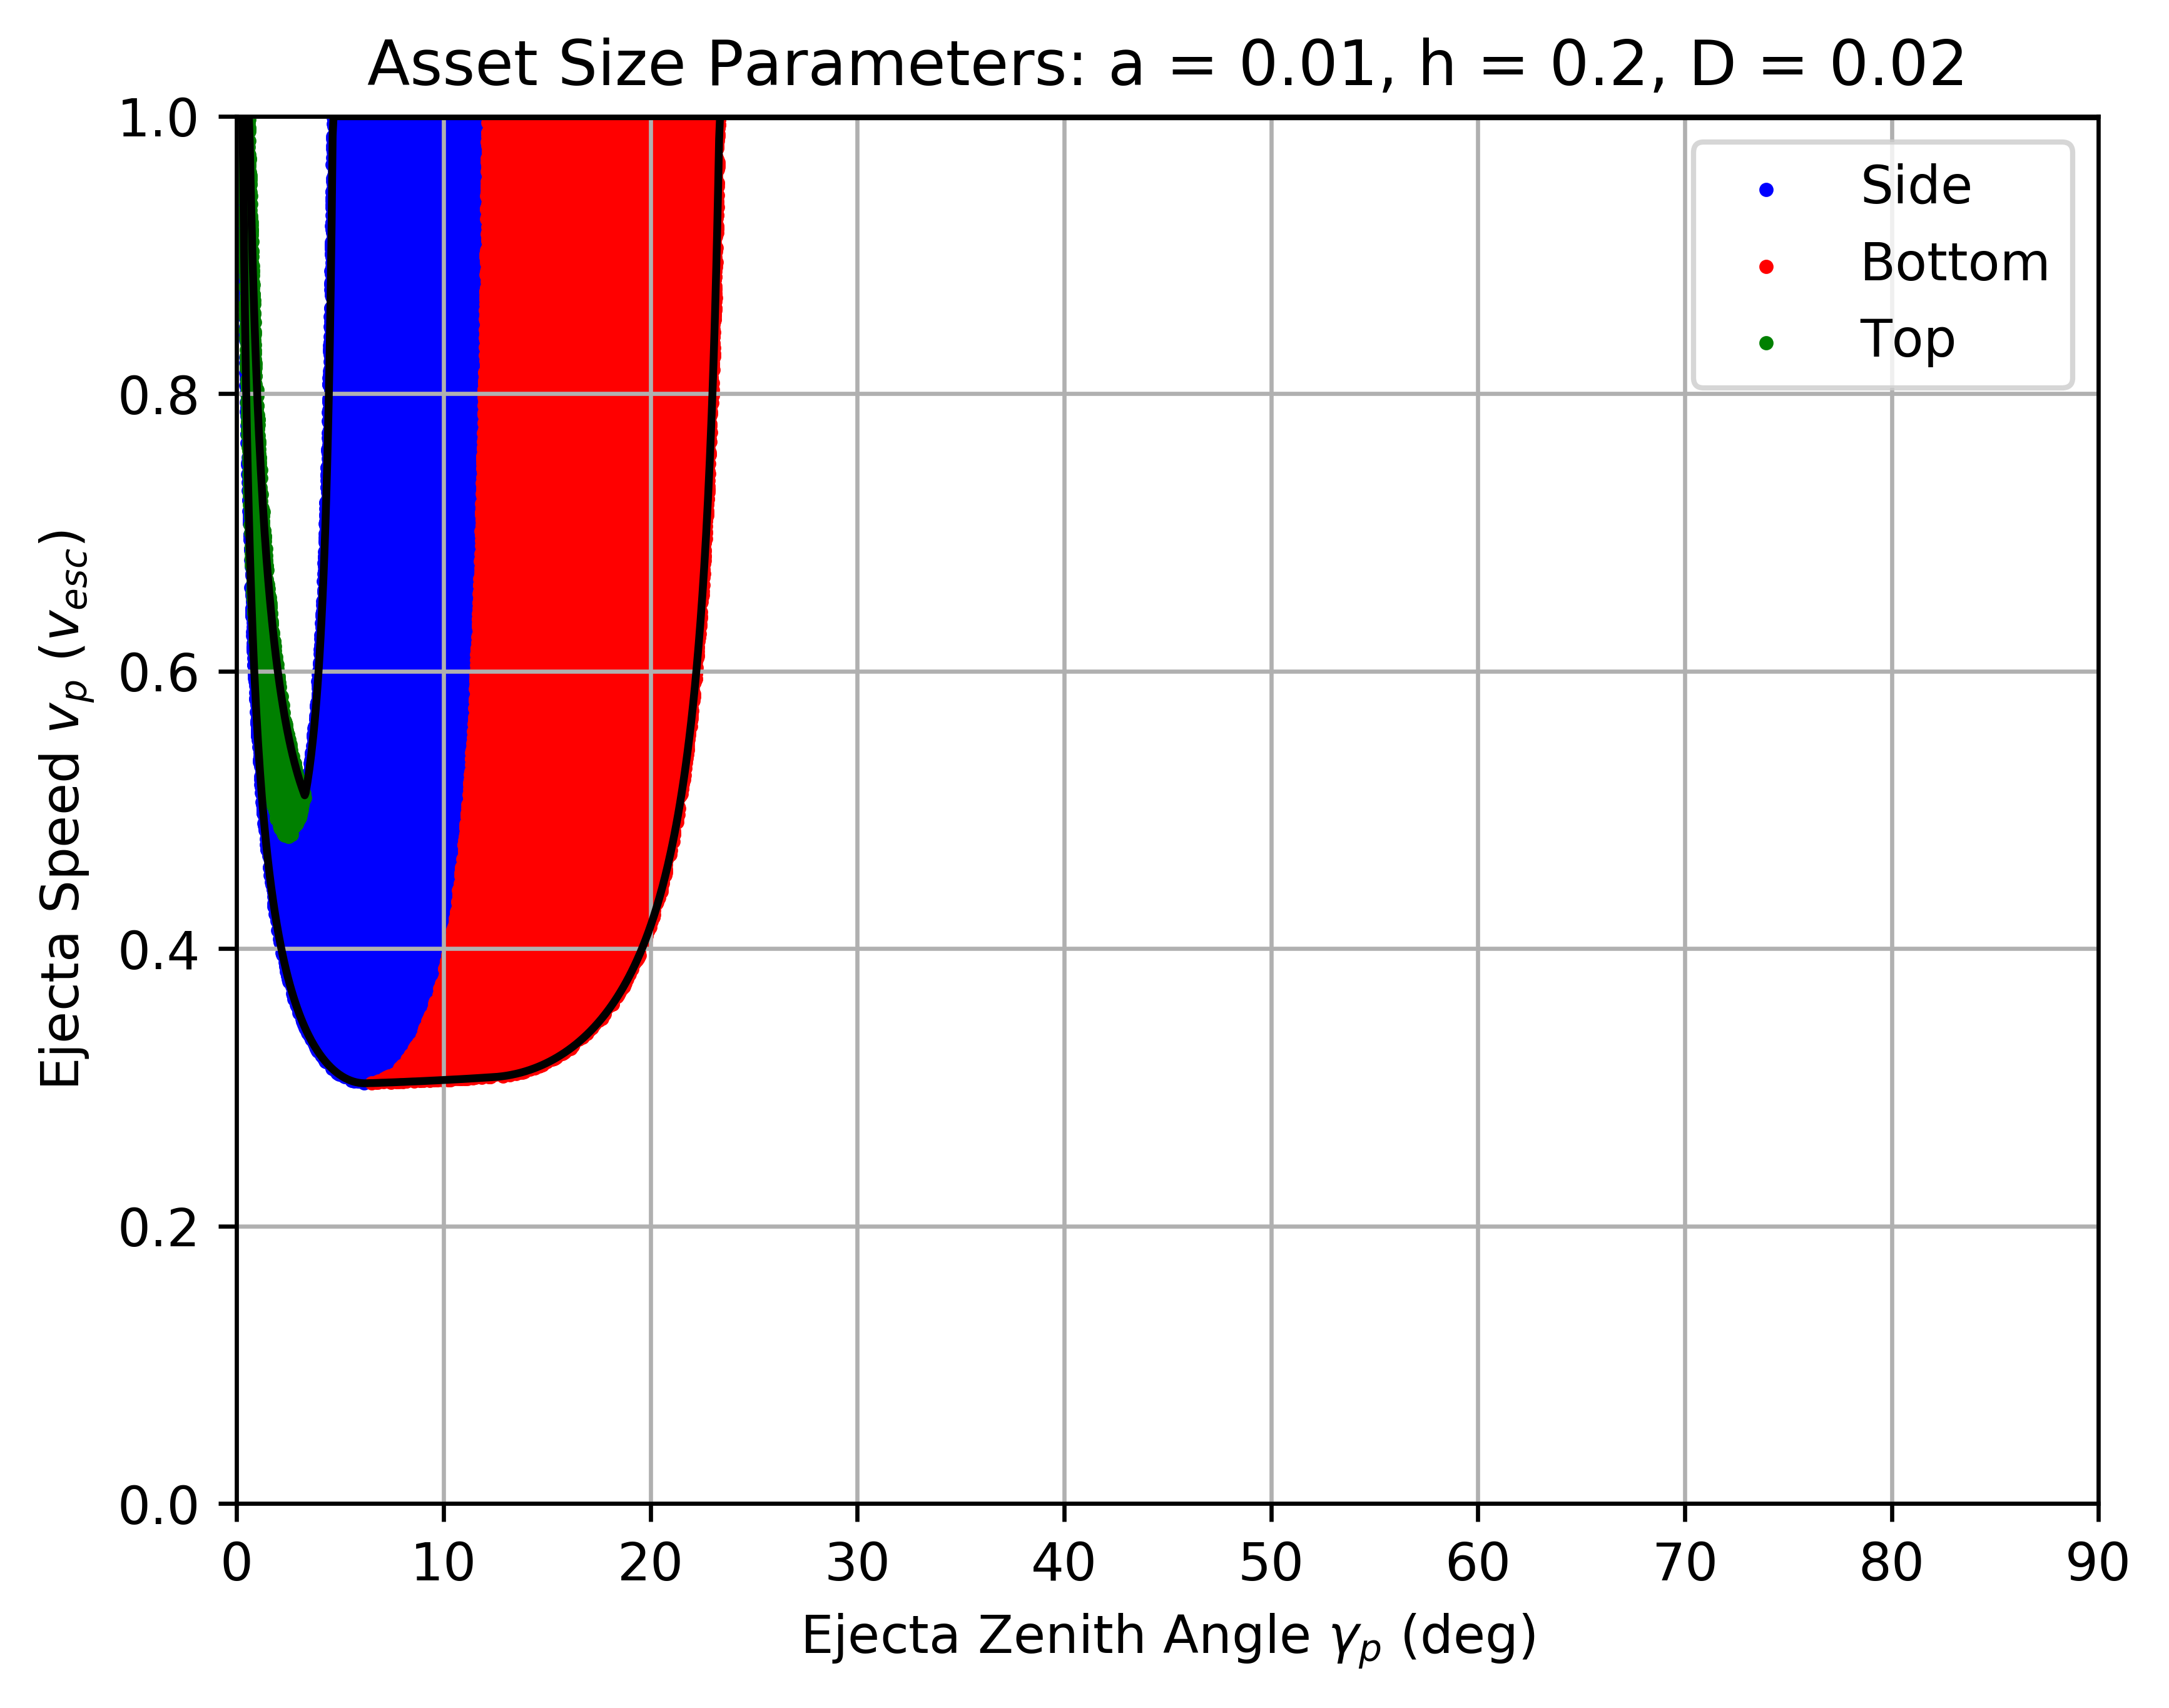
\includegraphics[width=.98\linewidth]{asset_speed_zenith_plot_1.100e+00_1.000e-02_2.000e-01_2.000e-02.png}  
		%\caption{Put your sub-caption here}
		\label{fig:sub-asset_speed_zenith_h2_4}
	\end{subfigure}
	\begin{subfigure}[t]{.32\textwidth}
		\centering
		% include fourth image
		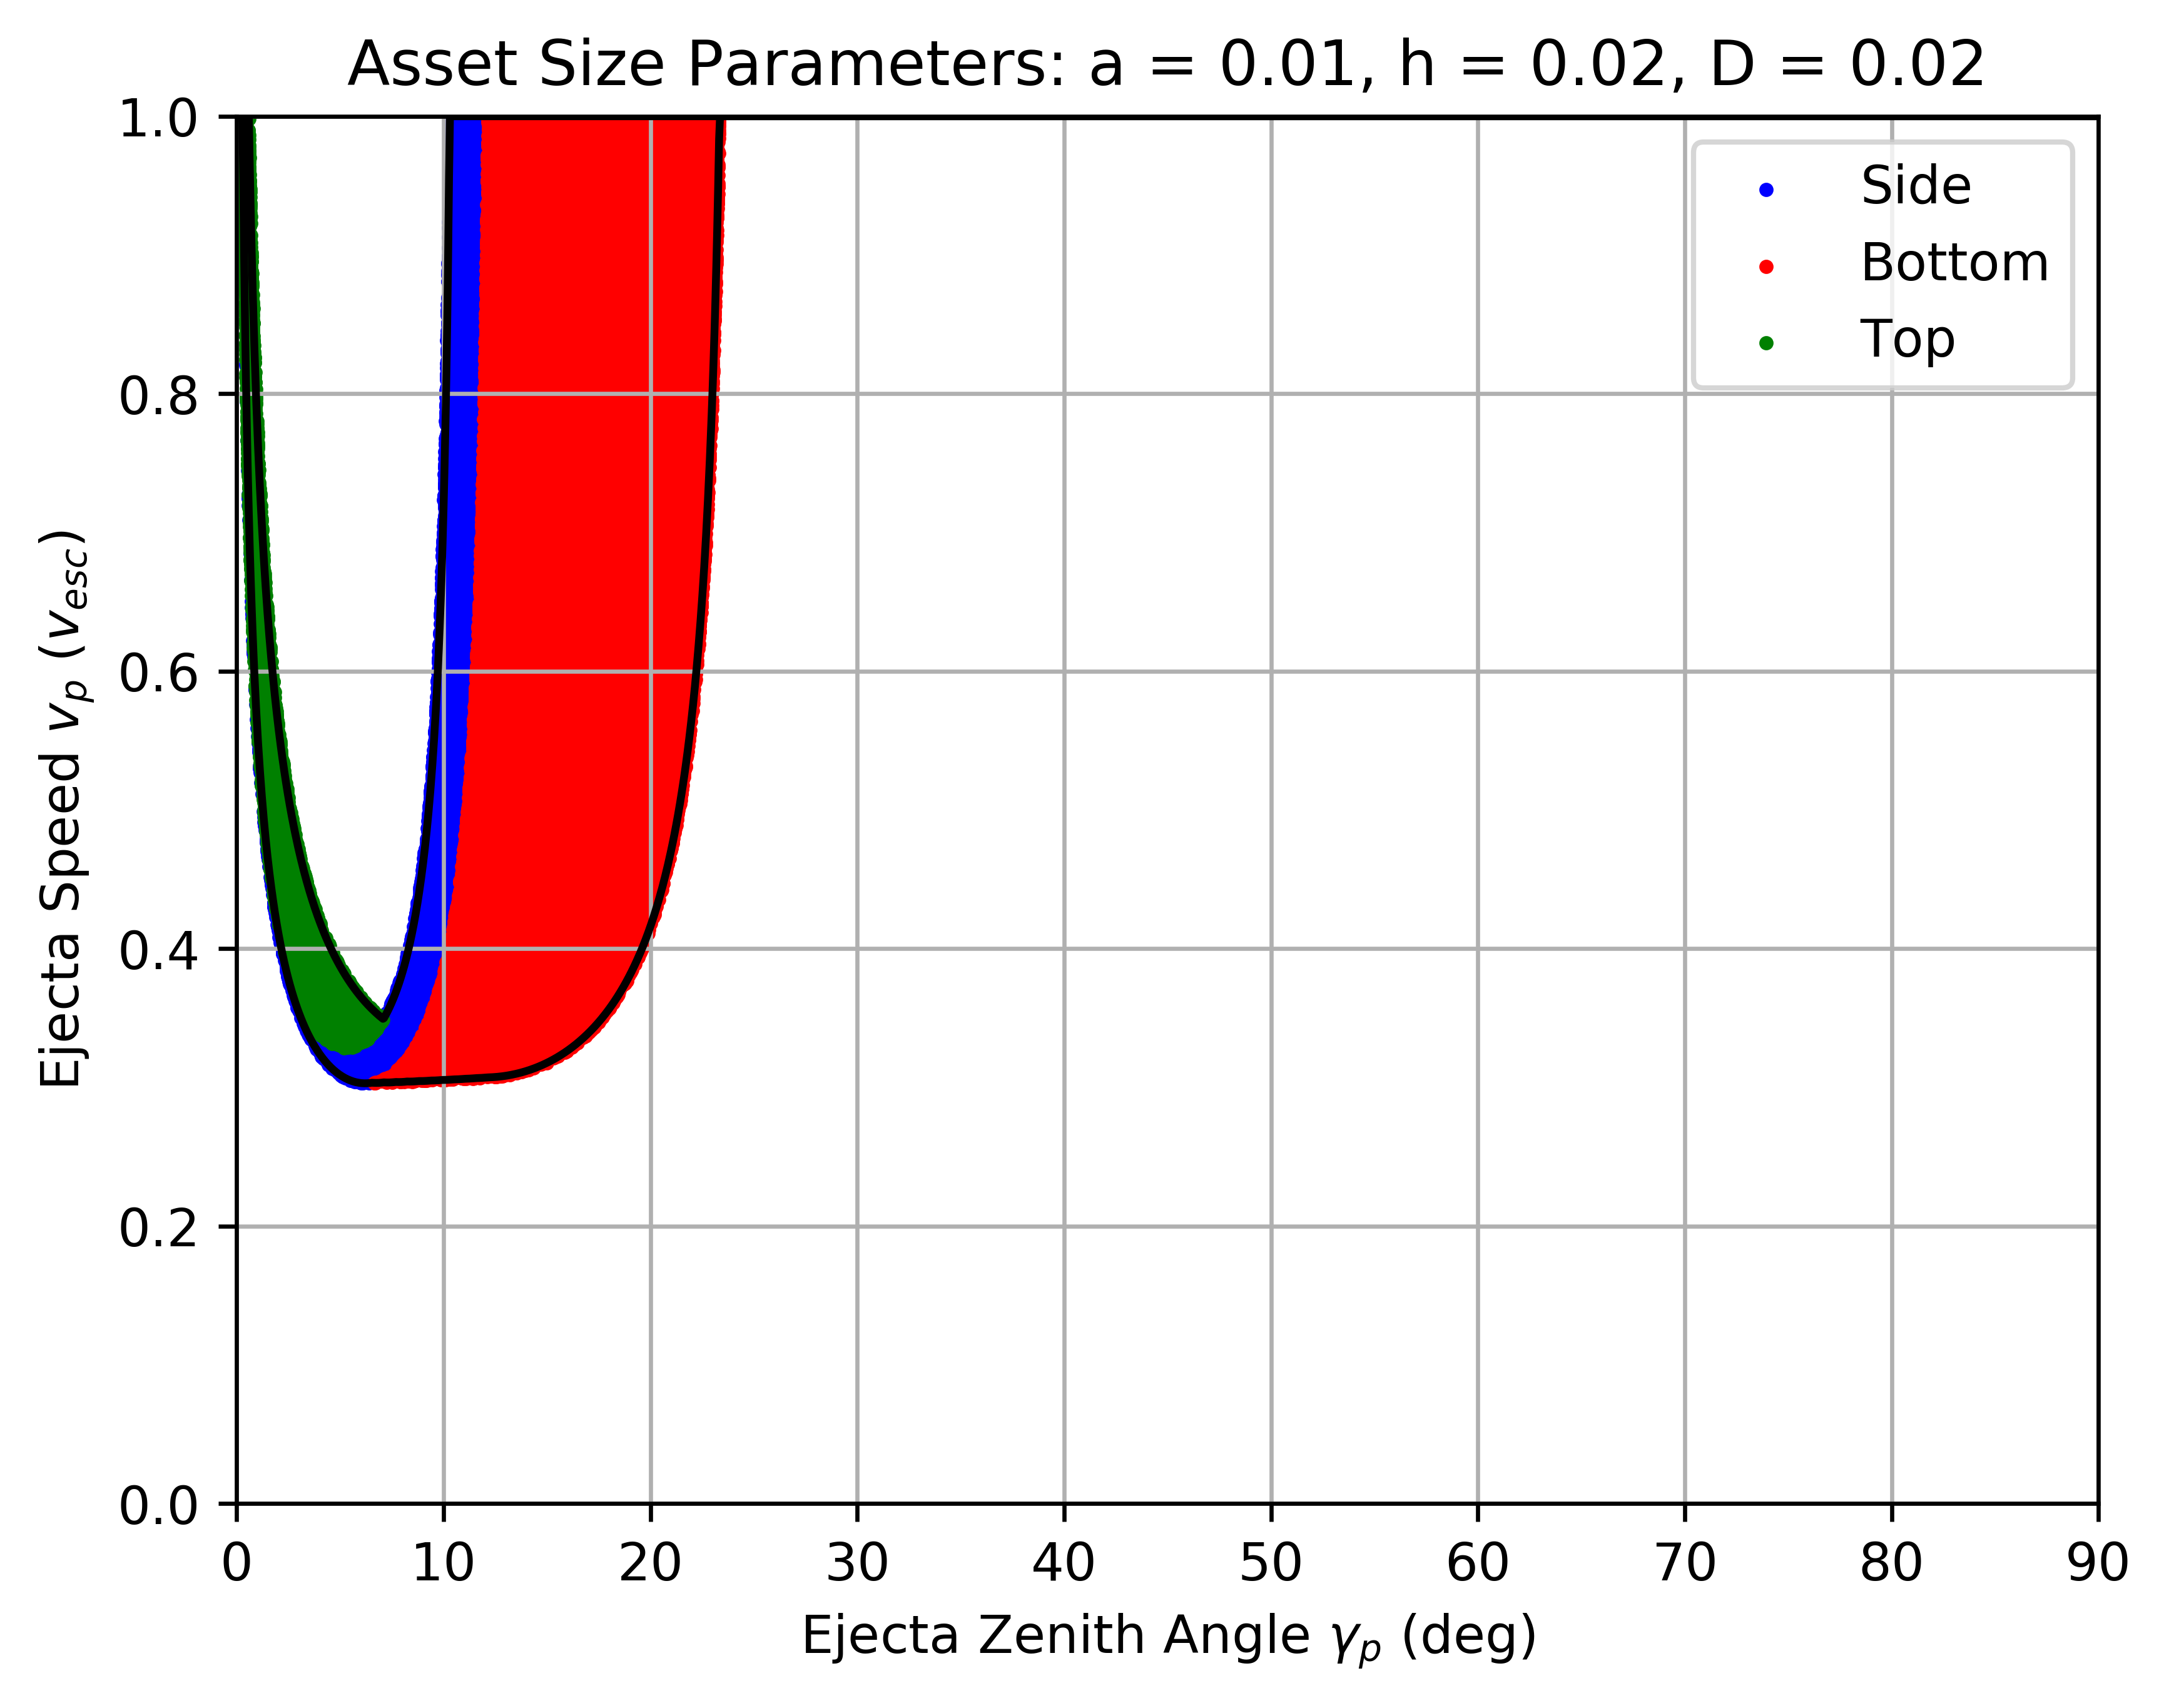
\includegraphics[width=.98\linewidth]{asset_speed_zenith_plot_1.100e+00_1.000e-02_2.000e-02_2.000e-02.png}  
		%\caption{Put your sub-caption here}
		\label{fig:sub-asset_speed_zenith_h2_5}
	\end{subfigure}
	\begin{subfigure}[t]{.32\textwidth}
		\centering
		% include fourth image
		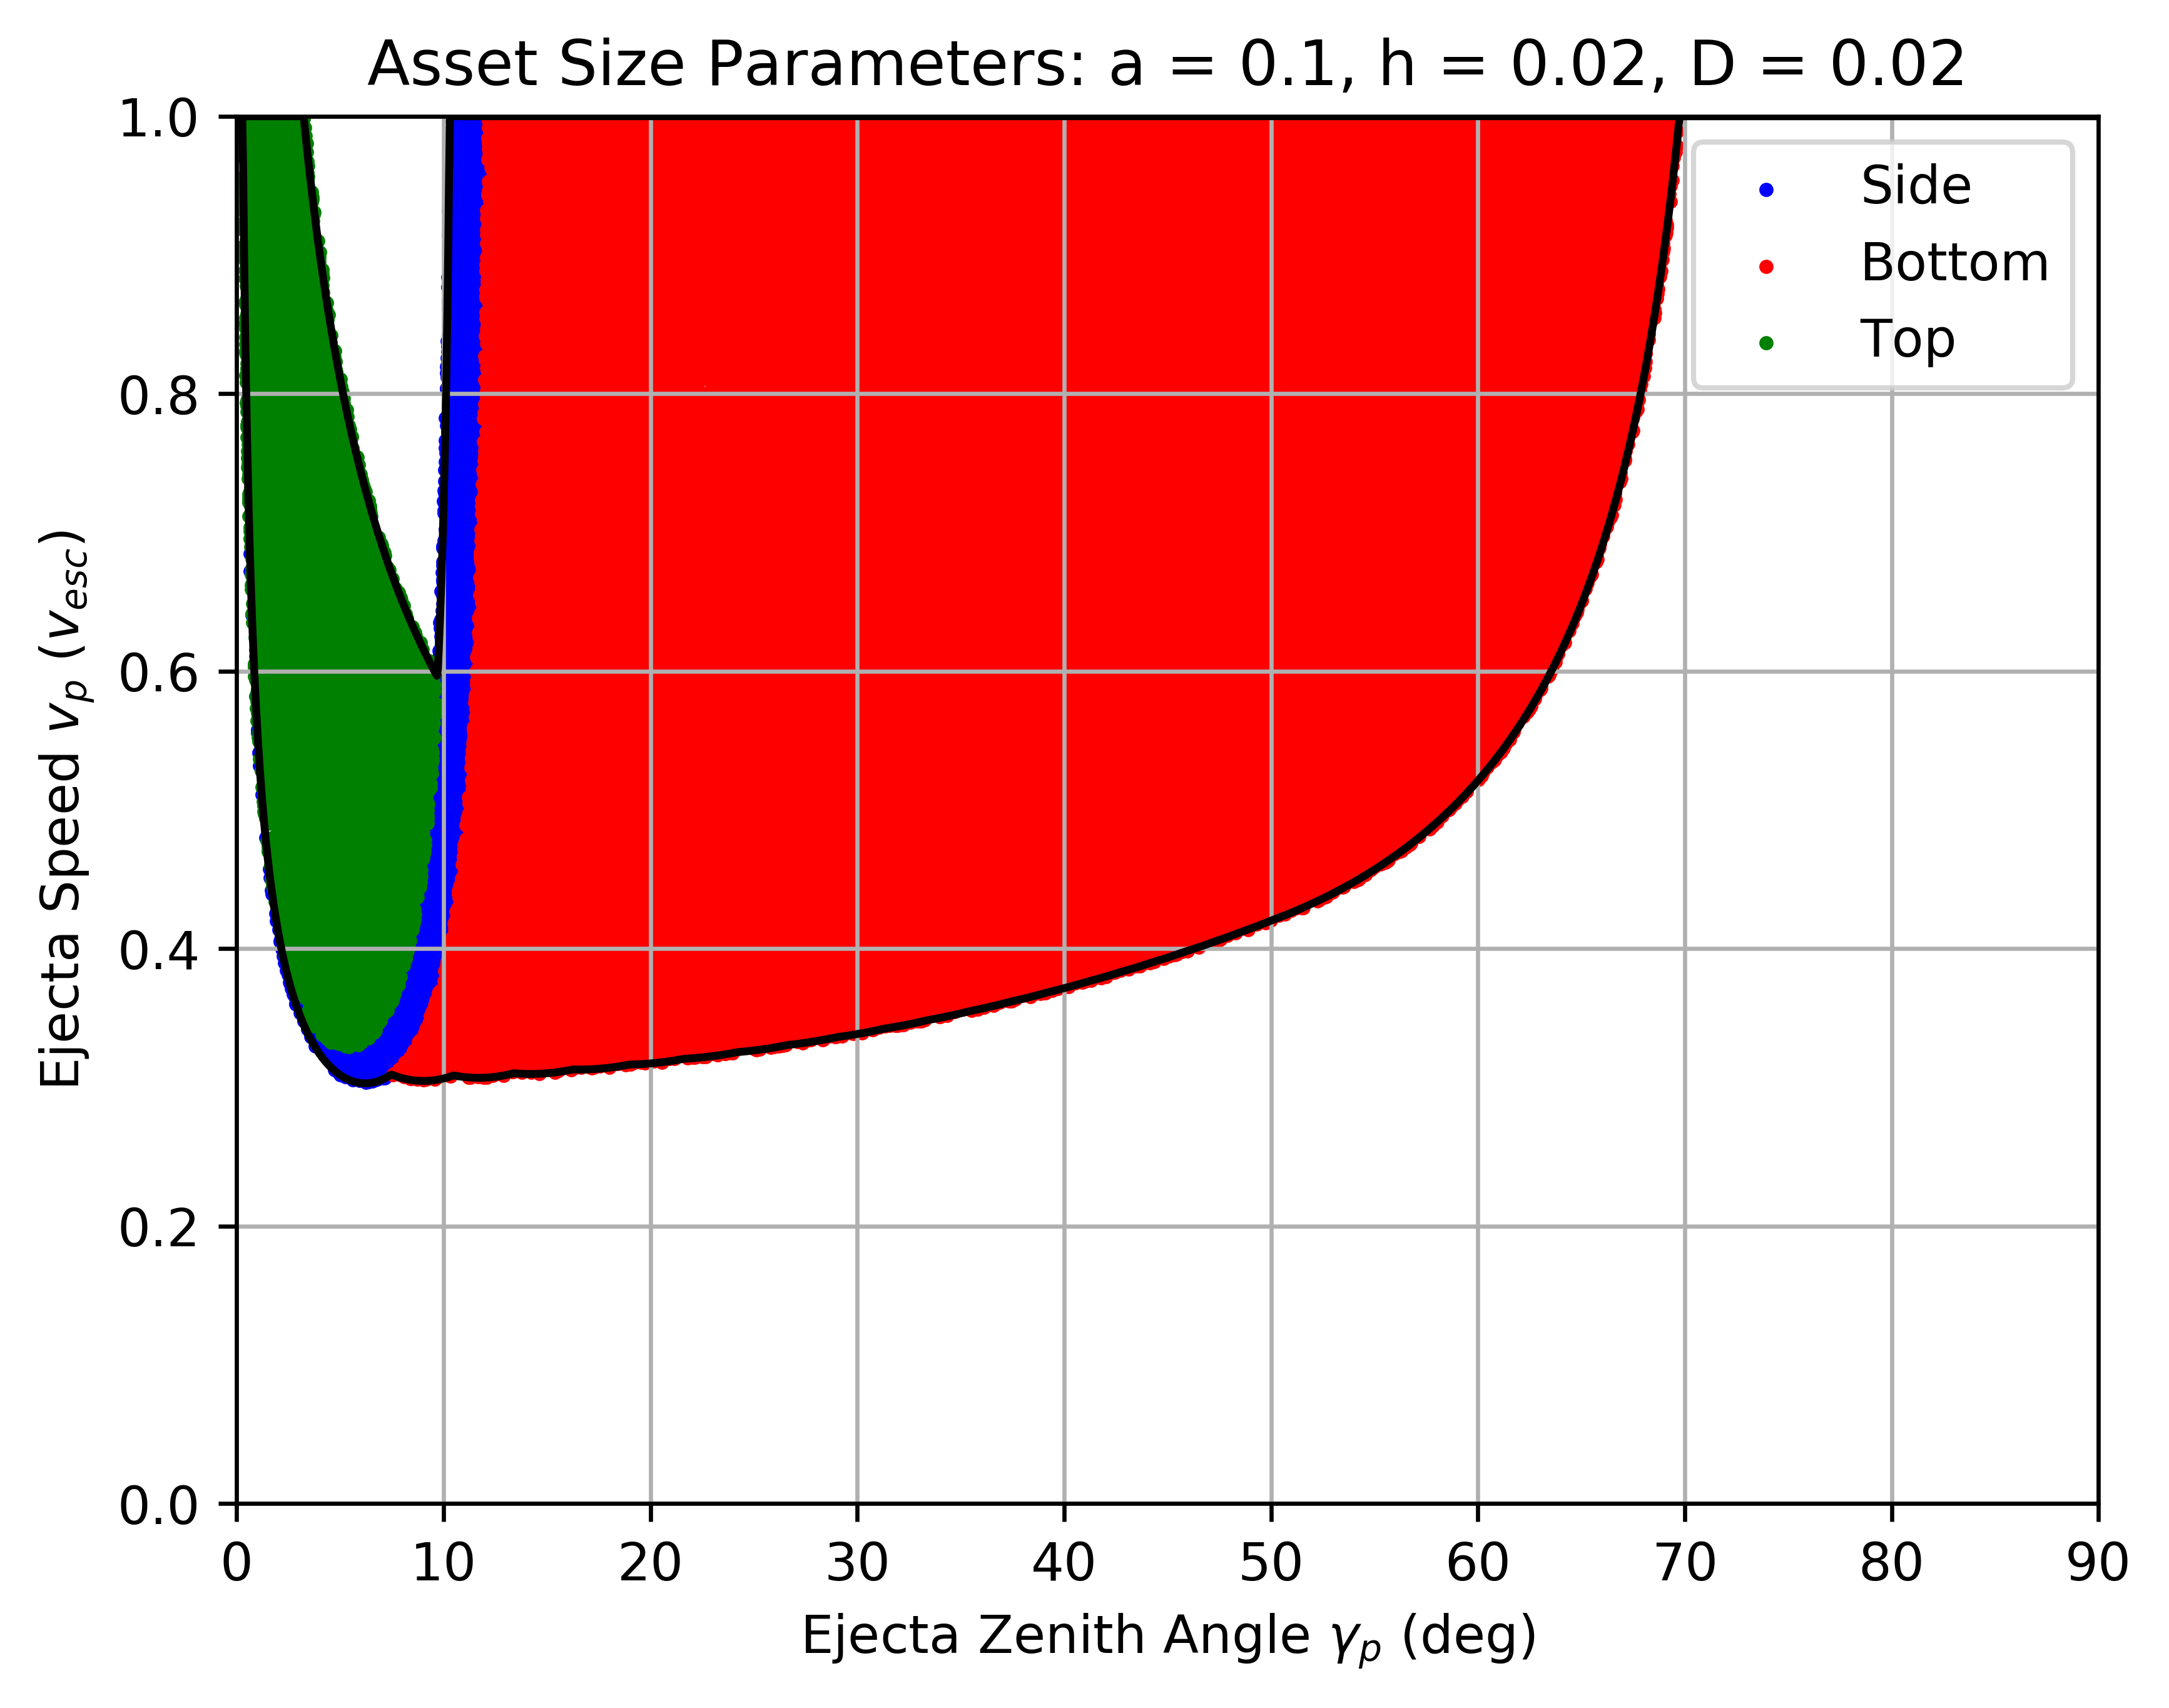
\includegraphics[width=.98\linewidth]{asset_speed_zenith_plot_1.100e+00_1.000e-01_2.000e-02_2.000e-02.png}  
		%\caption{Put your sub-caption here}
		\label{fig:sub-asset_speed_zenith_h2_6}
	\end{subfigure}
	
	
	\begin{subfigure}[t]{.32\textwidth}
		\centering
		% include third image
		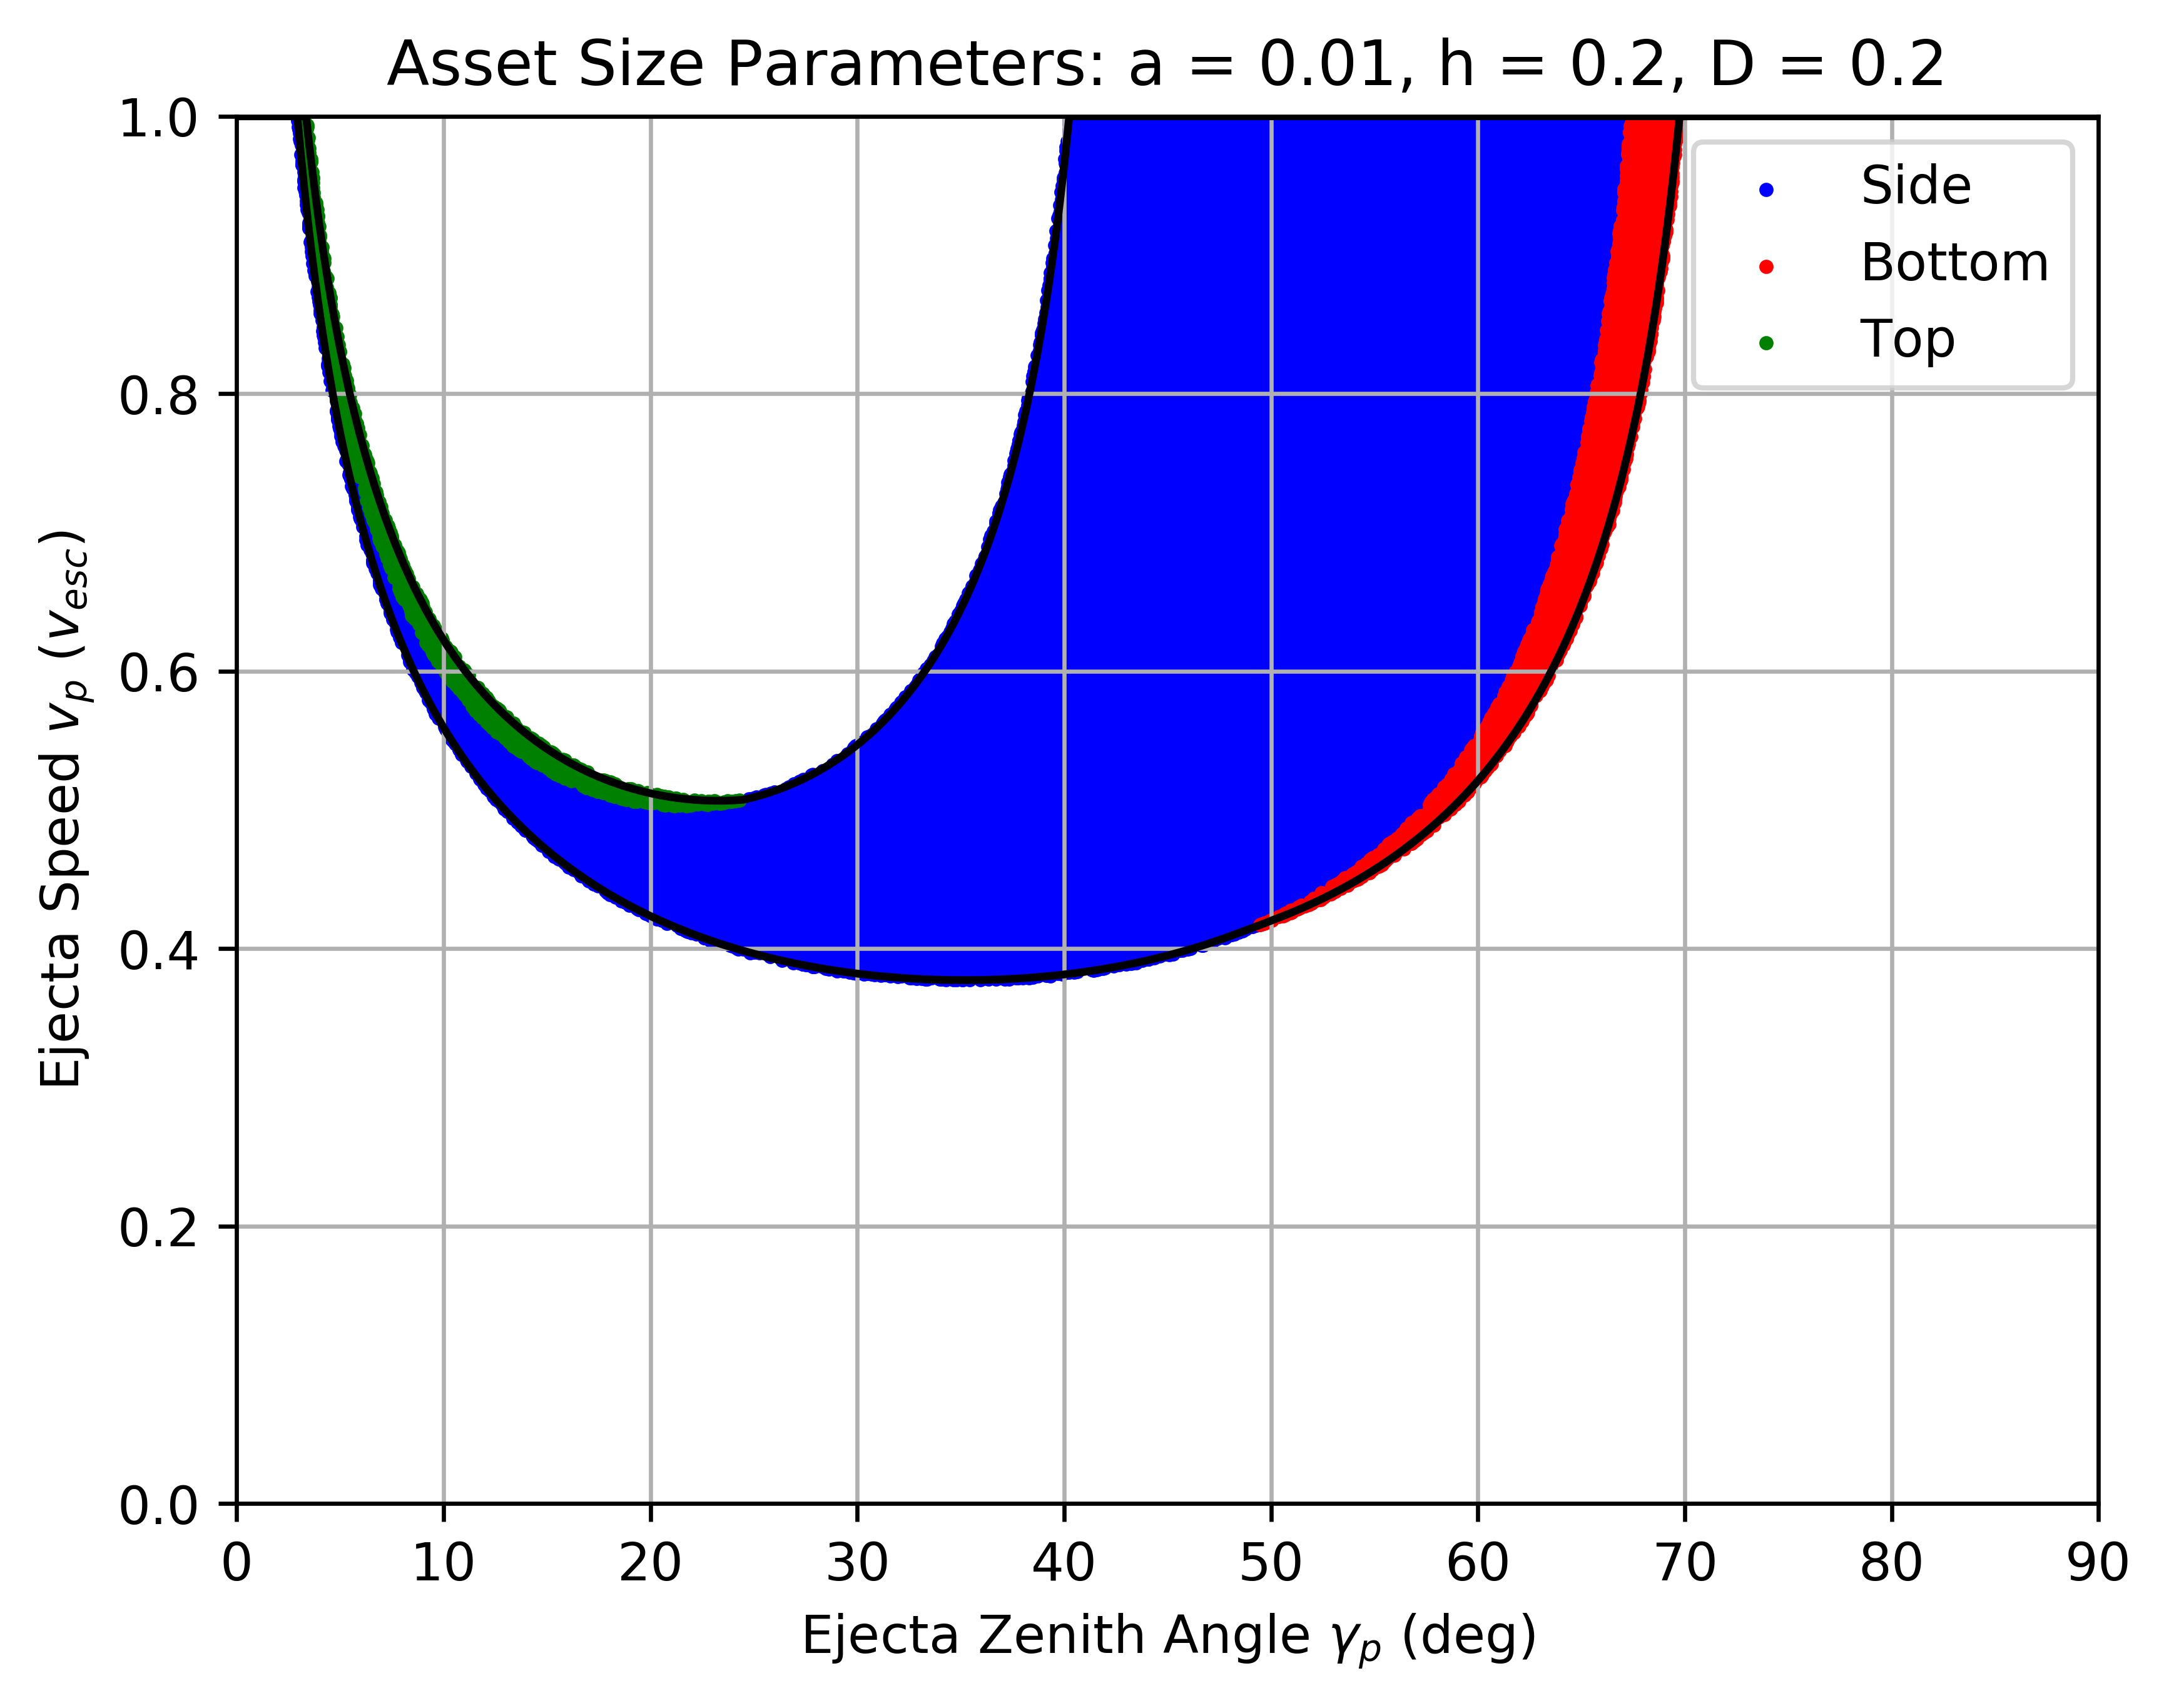
\includegraphics[width=.98\linewidth]{asset_speed_zenith_plot_1.100e+00_1.000e-02_2.000e-01_2.000e-01.png}  
		%\caption{Put your sub-caption here}
		\label{fig:sub-asset_speed_zenith_h2_7}
	\end{subfigure}
	\begin{subfigure}[t]{.32\textwidth}
		\centering
		% include fourth image
		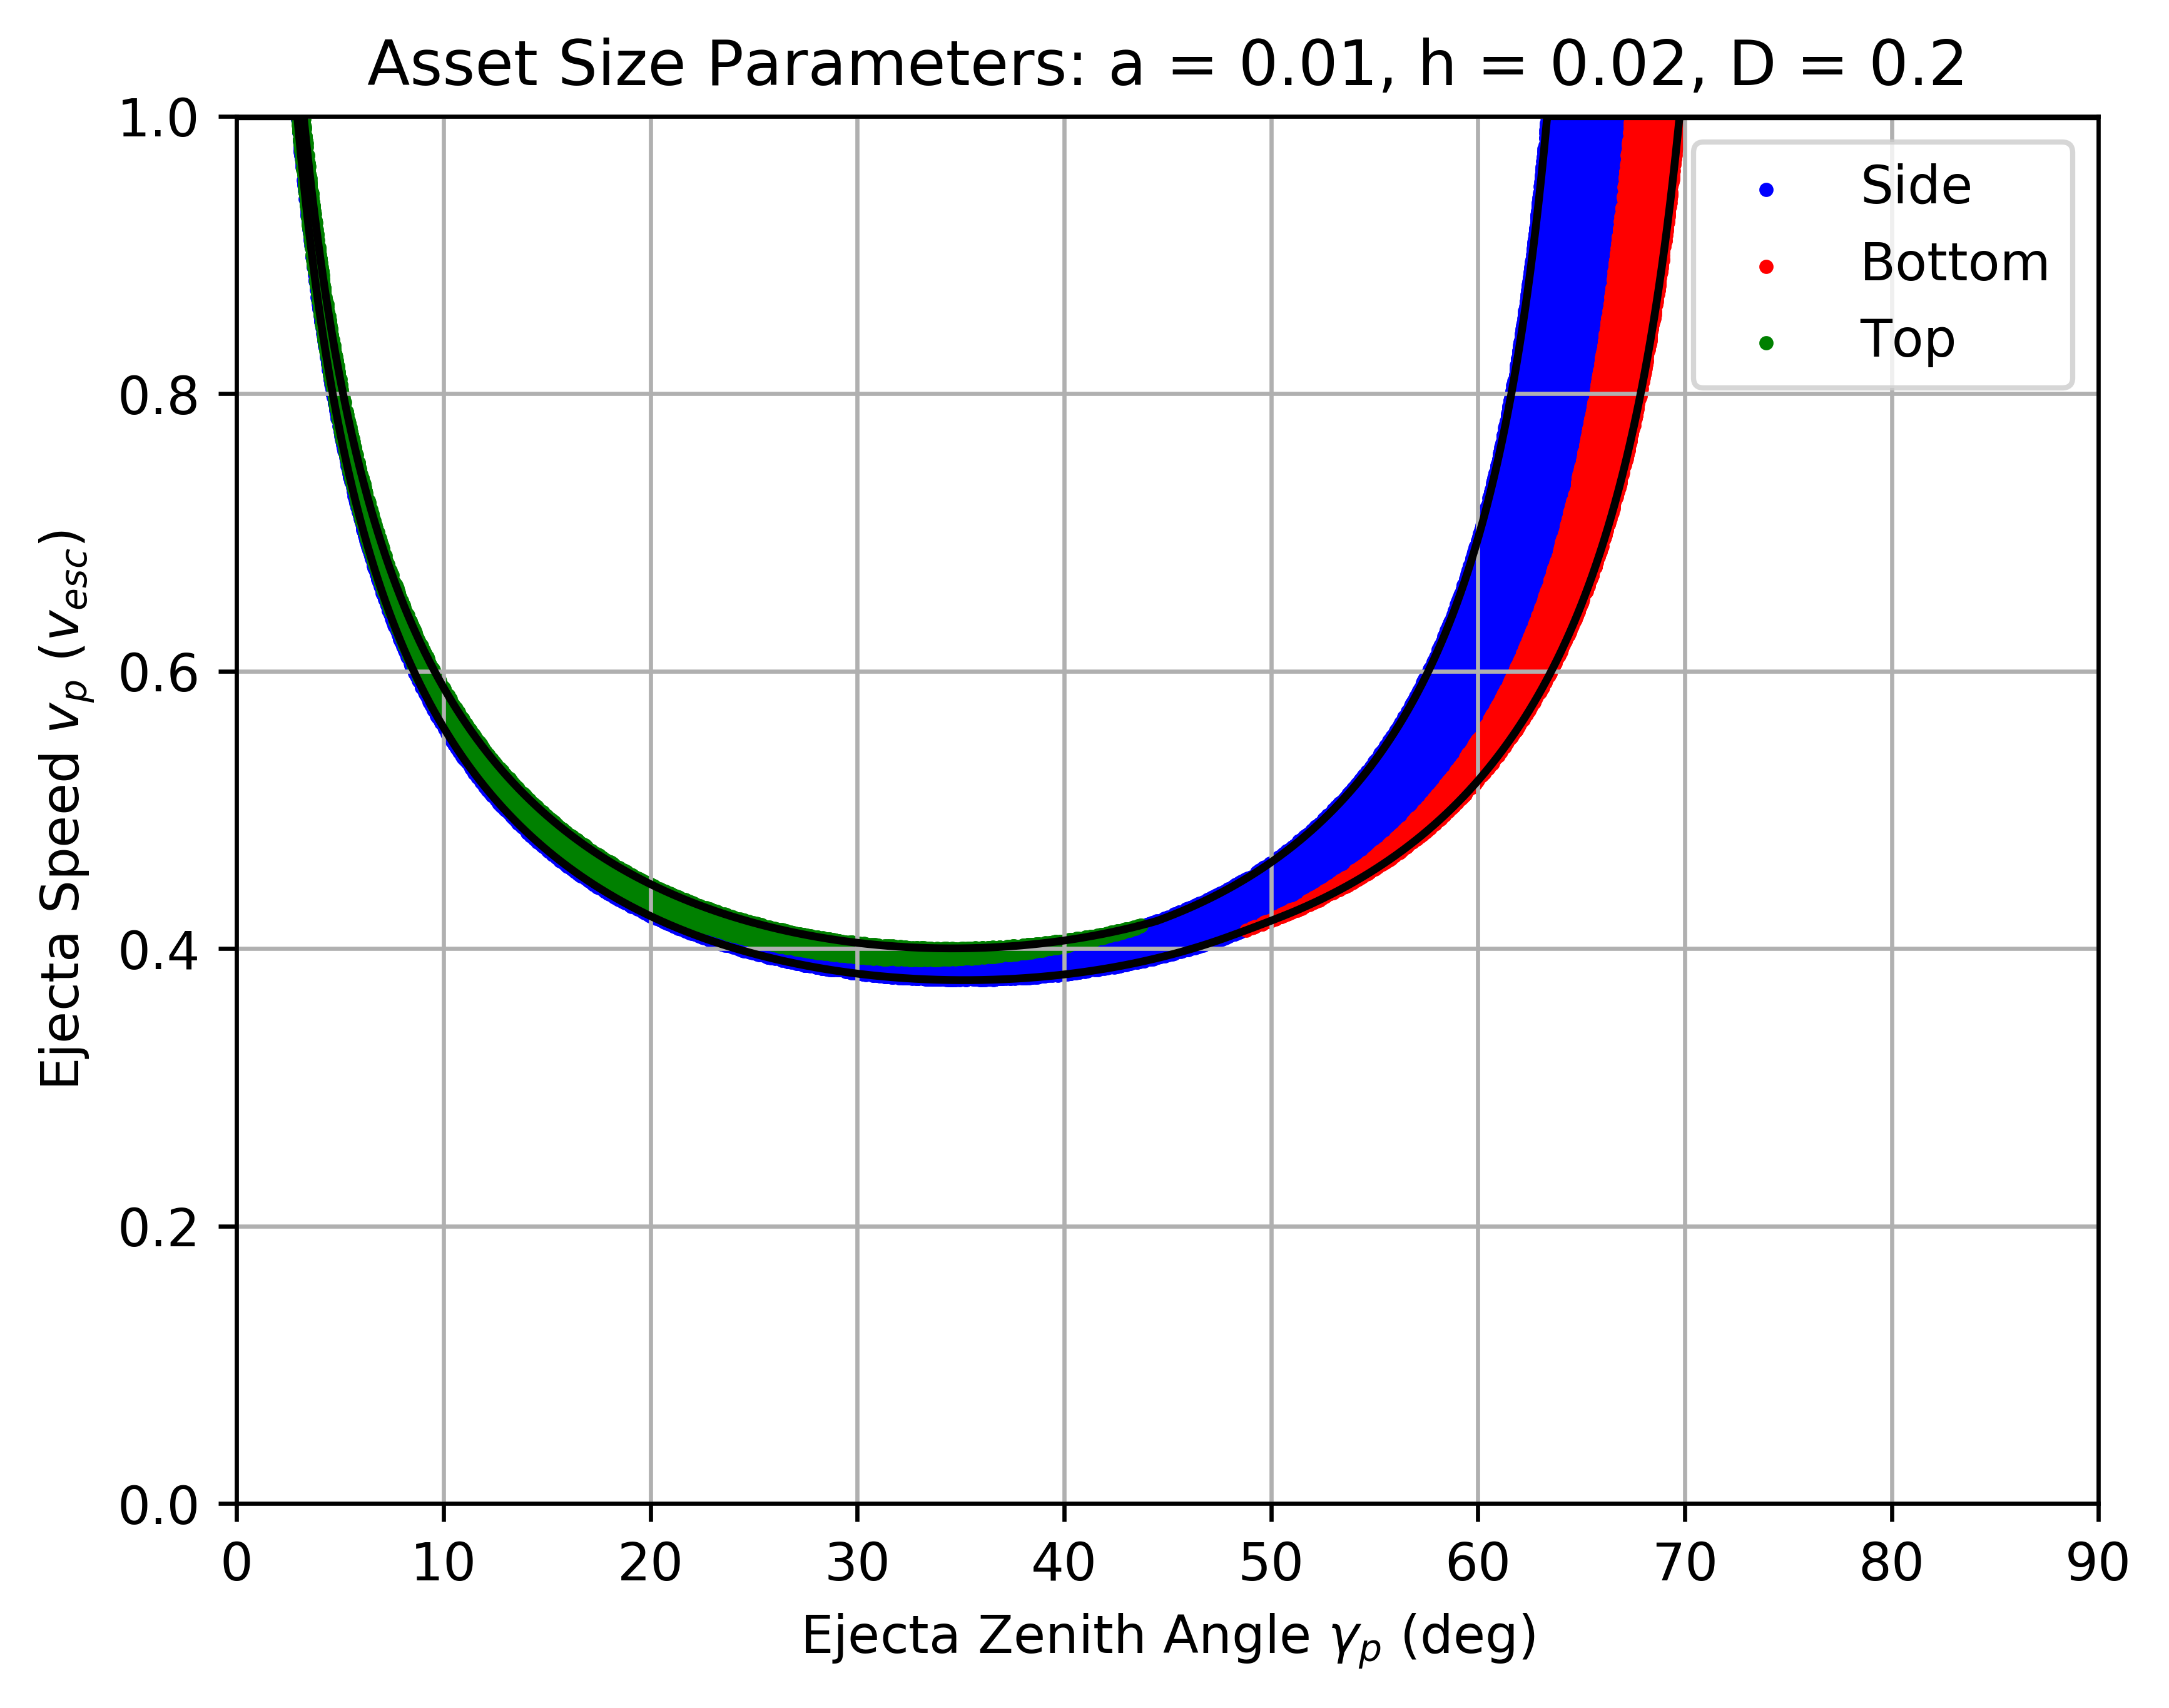
\includegraphics[width=.98\linewidth]{asset_speed_zenith_plot_1.100e+00_1.000e-02_2.000e-02_2.000e-01.png}  
		%\caption{Put your sub-caption here}
		\label{fig:sub-asset_speed_zenith_h2_8}
	\end{subfigure}
	\begin{subfigure}[t]{.32\textwidth}
		\centering
		% include fourth image
		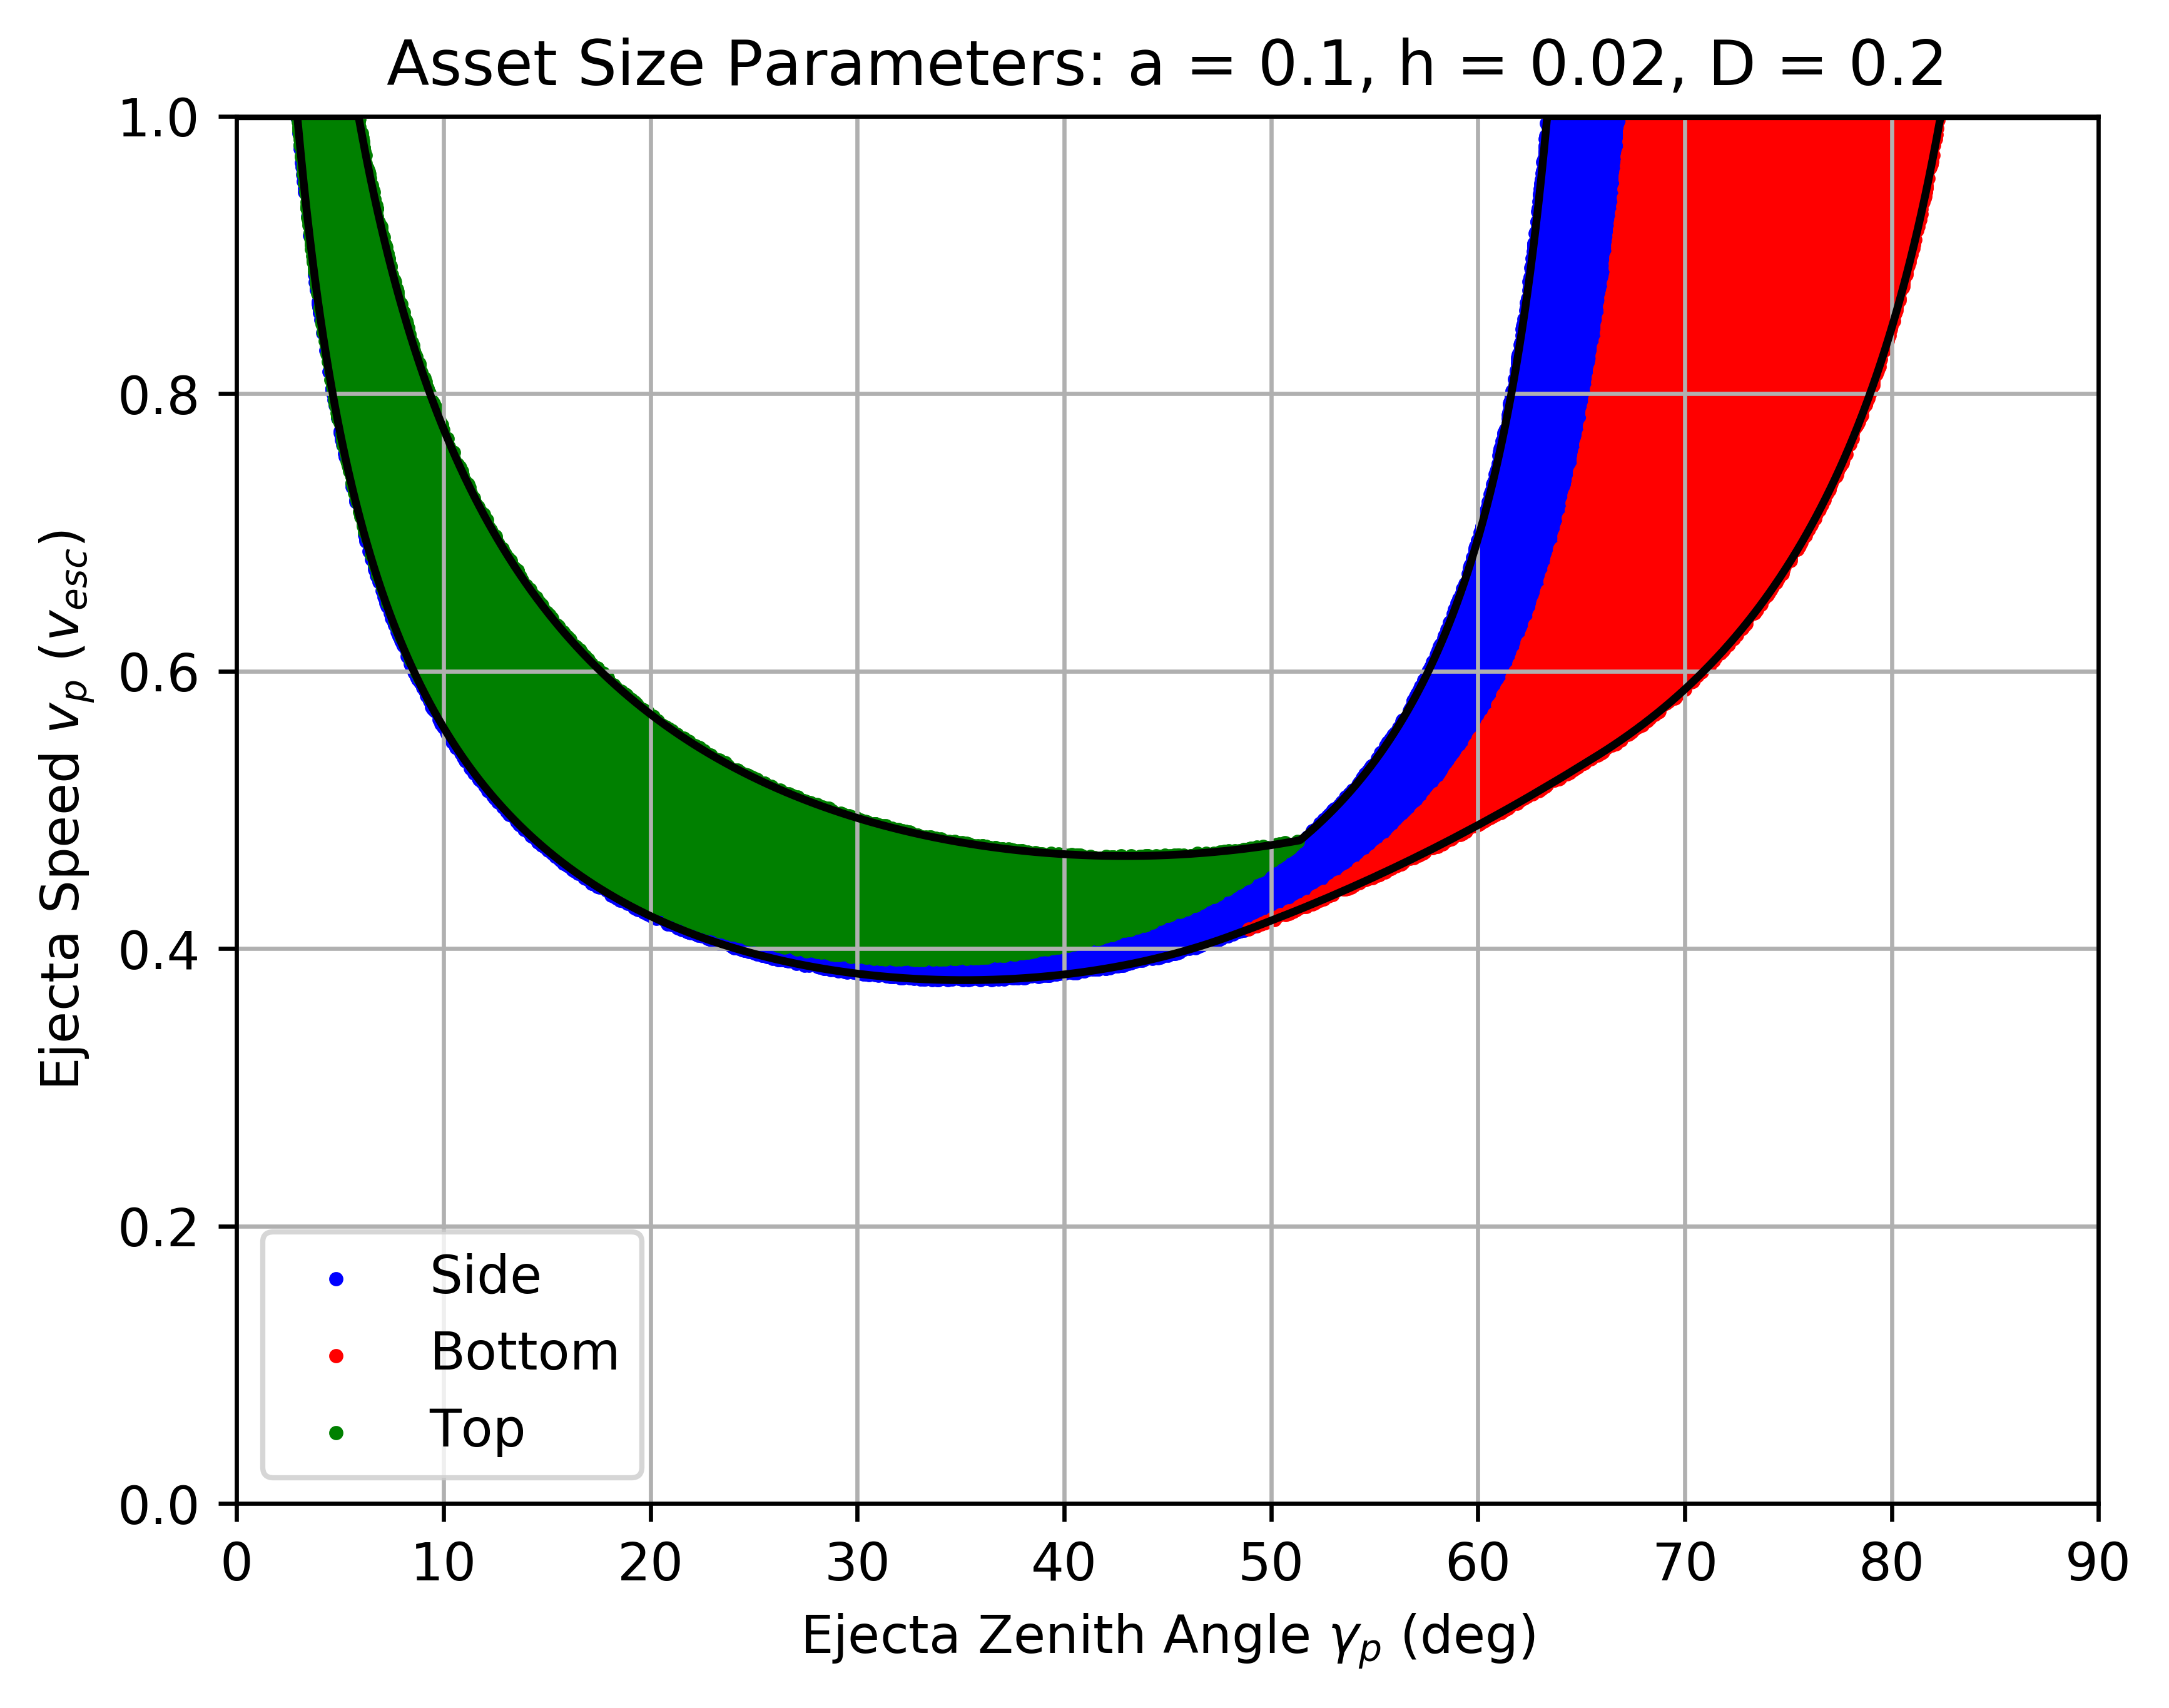
\includegraphics[width=.98\linewidth]{asset_speed_zenith_plot_1.100e+00_1.000e-01_2.000e-02_2.000e-01.png}  
		%\caption{Put your sub-caption here}
		\label{fig:sub-asset_speed_zenith_h2_9}
	\end{subfigure}
	
	\begin{subfigure}[t]{.32\textwidth}
		\centering
		% include third image
		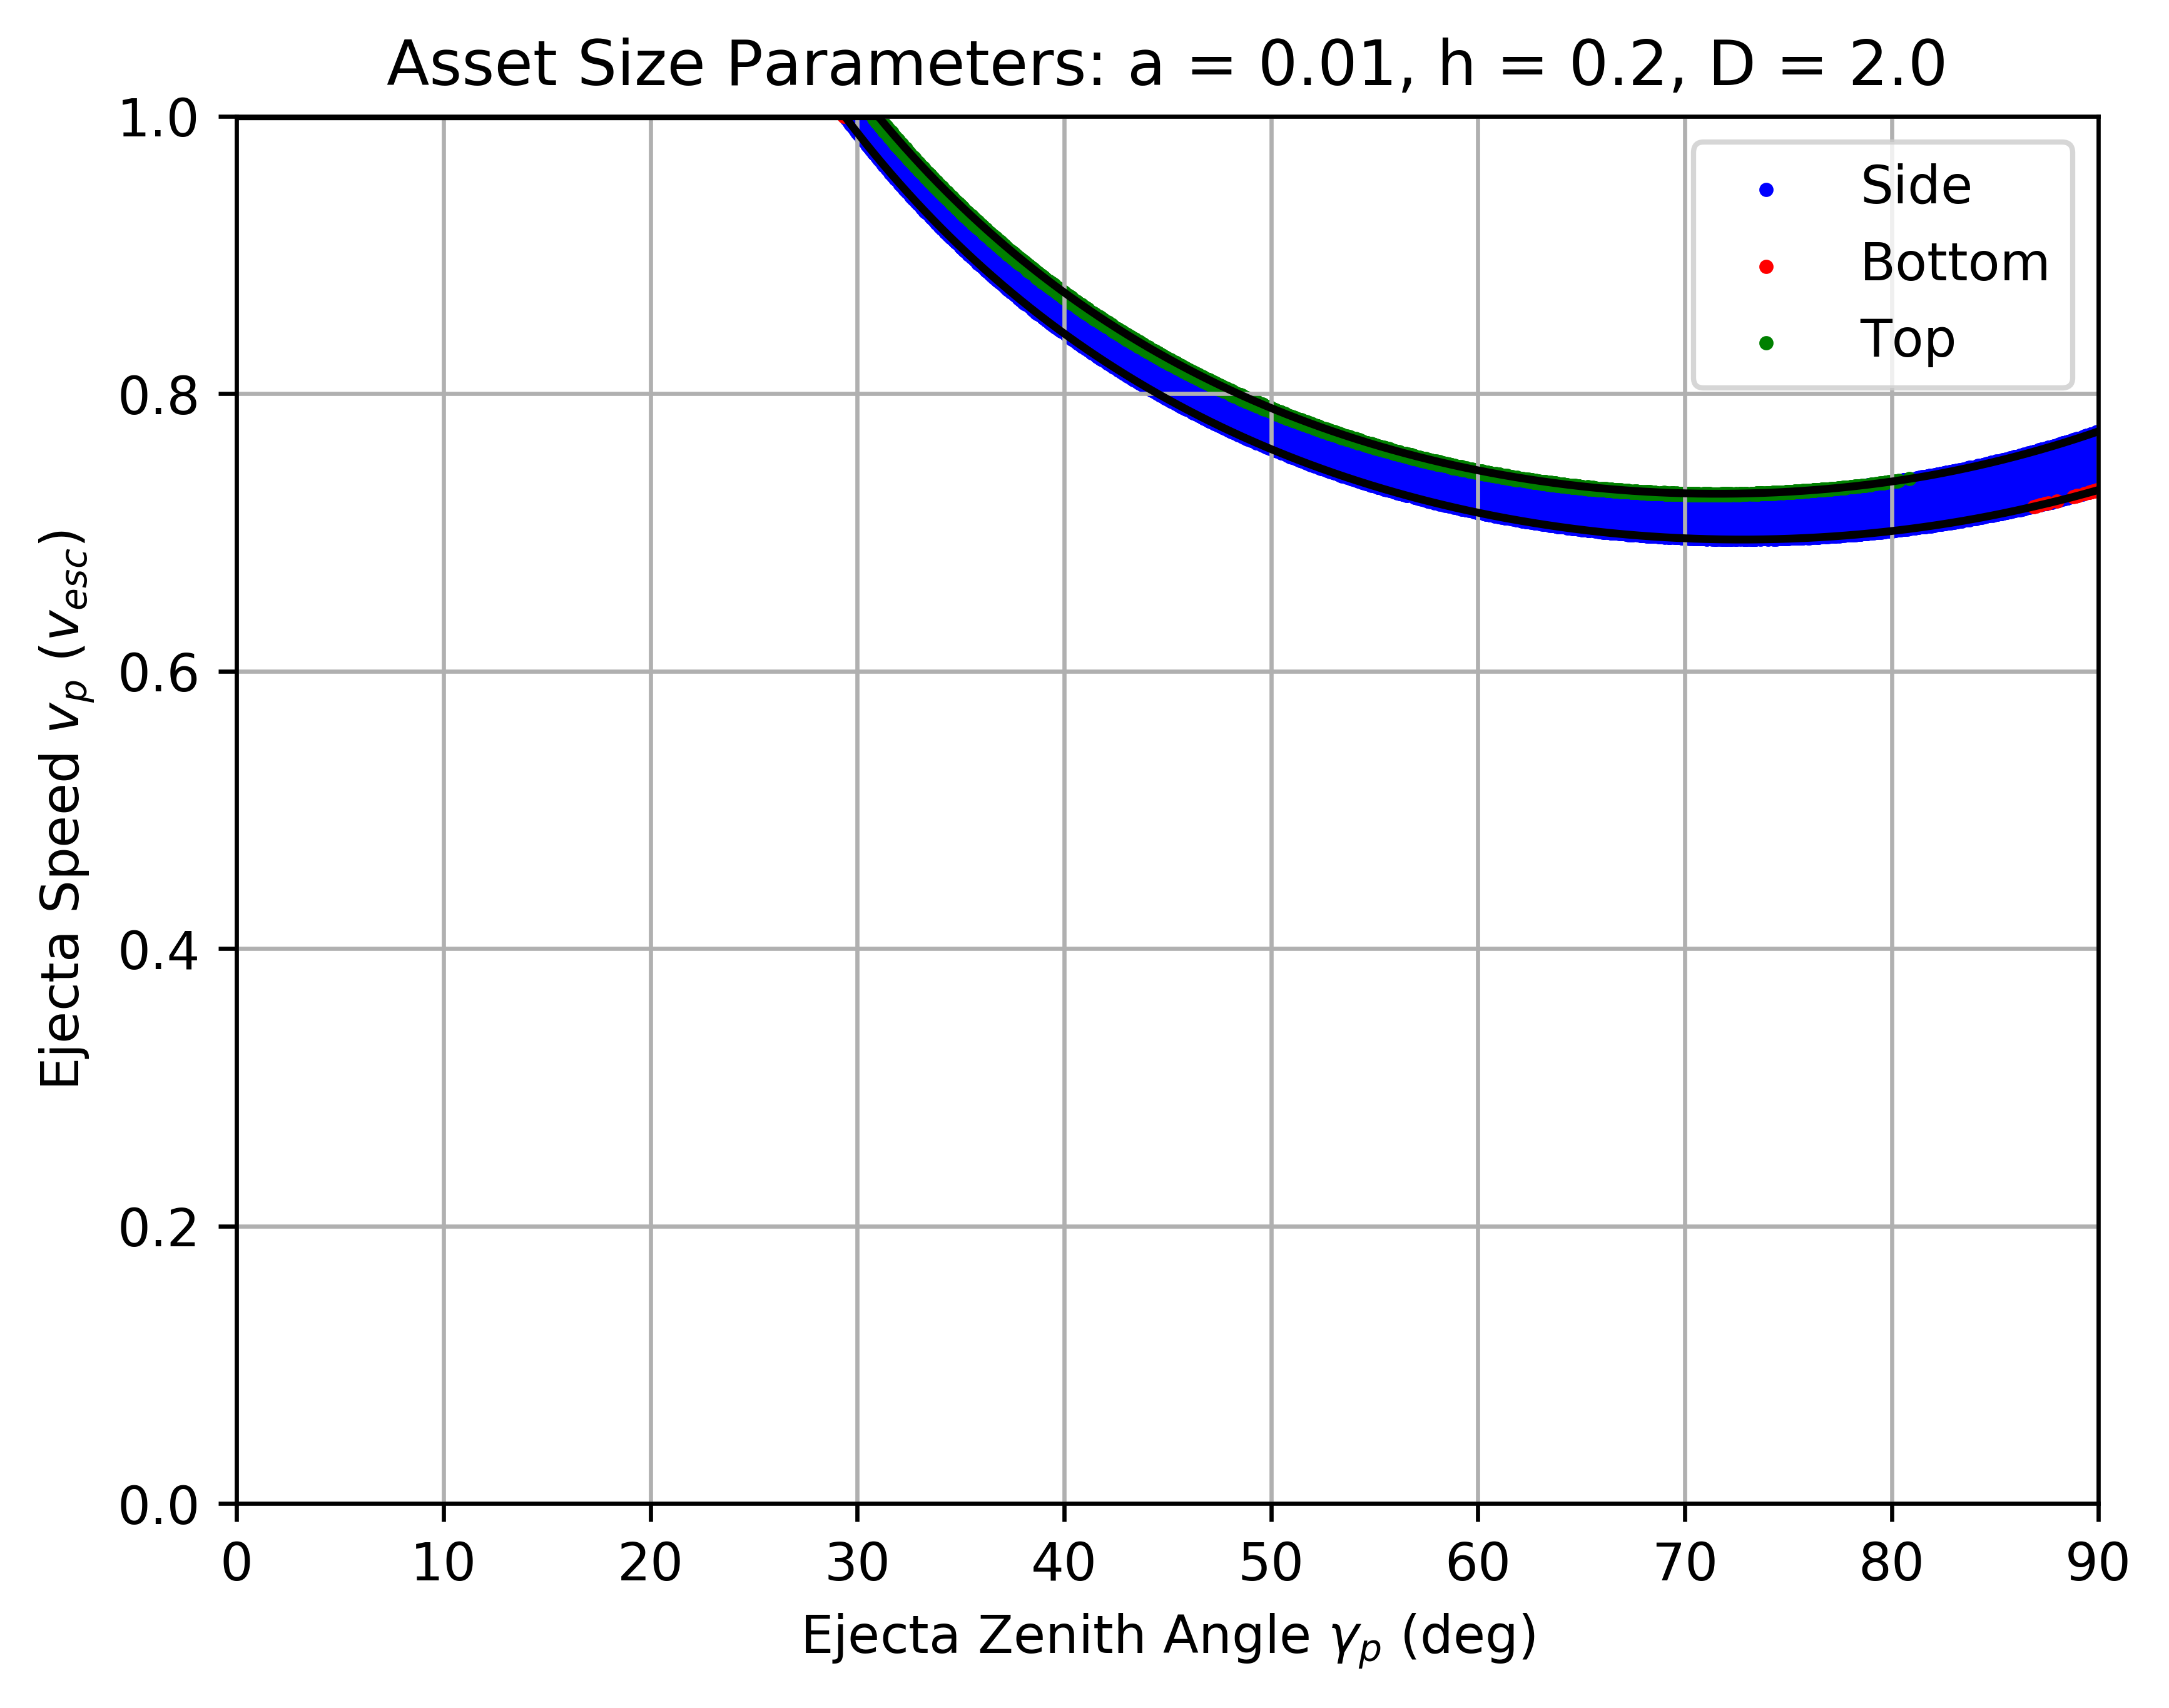
\includegraphics[width=.98\linewidth]{asset_speed_zenith_plot_1.100e+00_1.000e-02_2.000e-01_2.000e+00.png}  
		%\caption{Put your sub-caption here}
		\label{fig:sub-asset_speed_zenith_h2_10}
	\end{subfigure}
	\begin{subfigure}[t]{.32\textwidth}
		\centering
		% include fourth image
		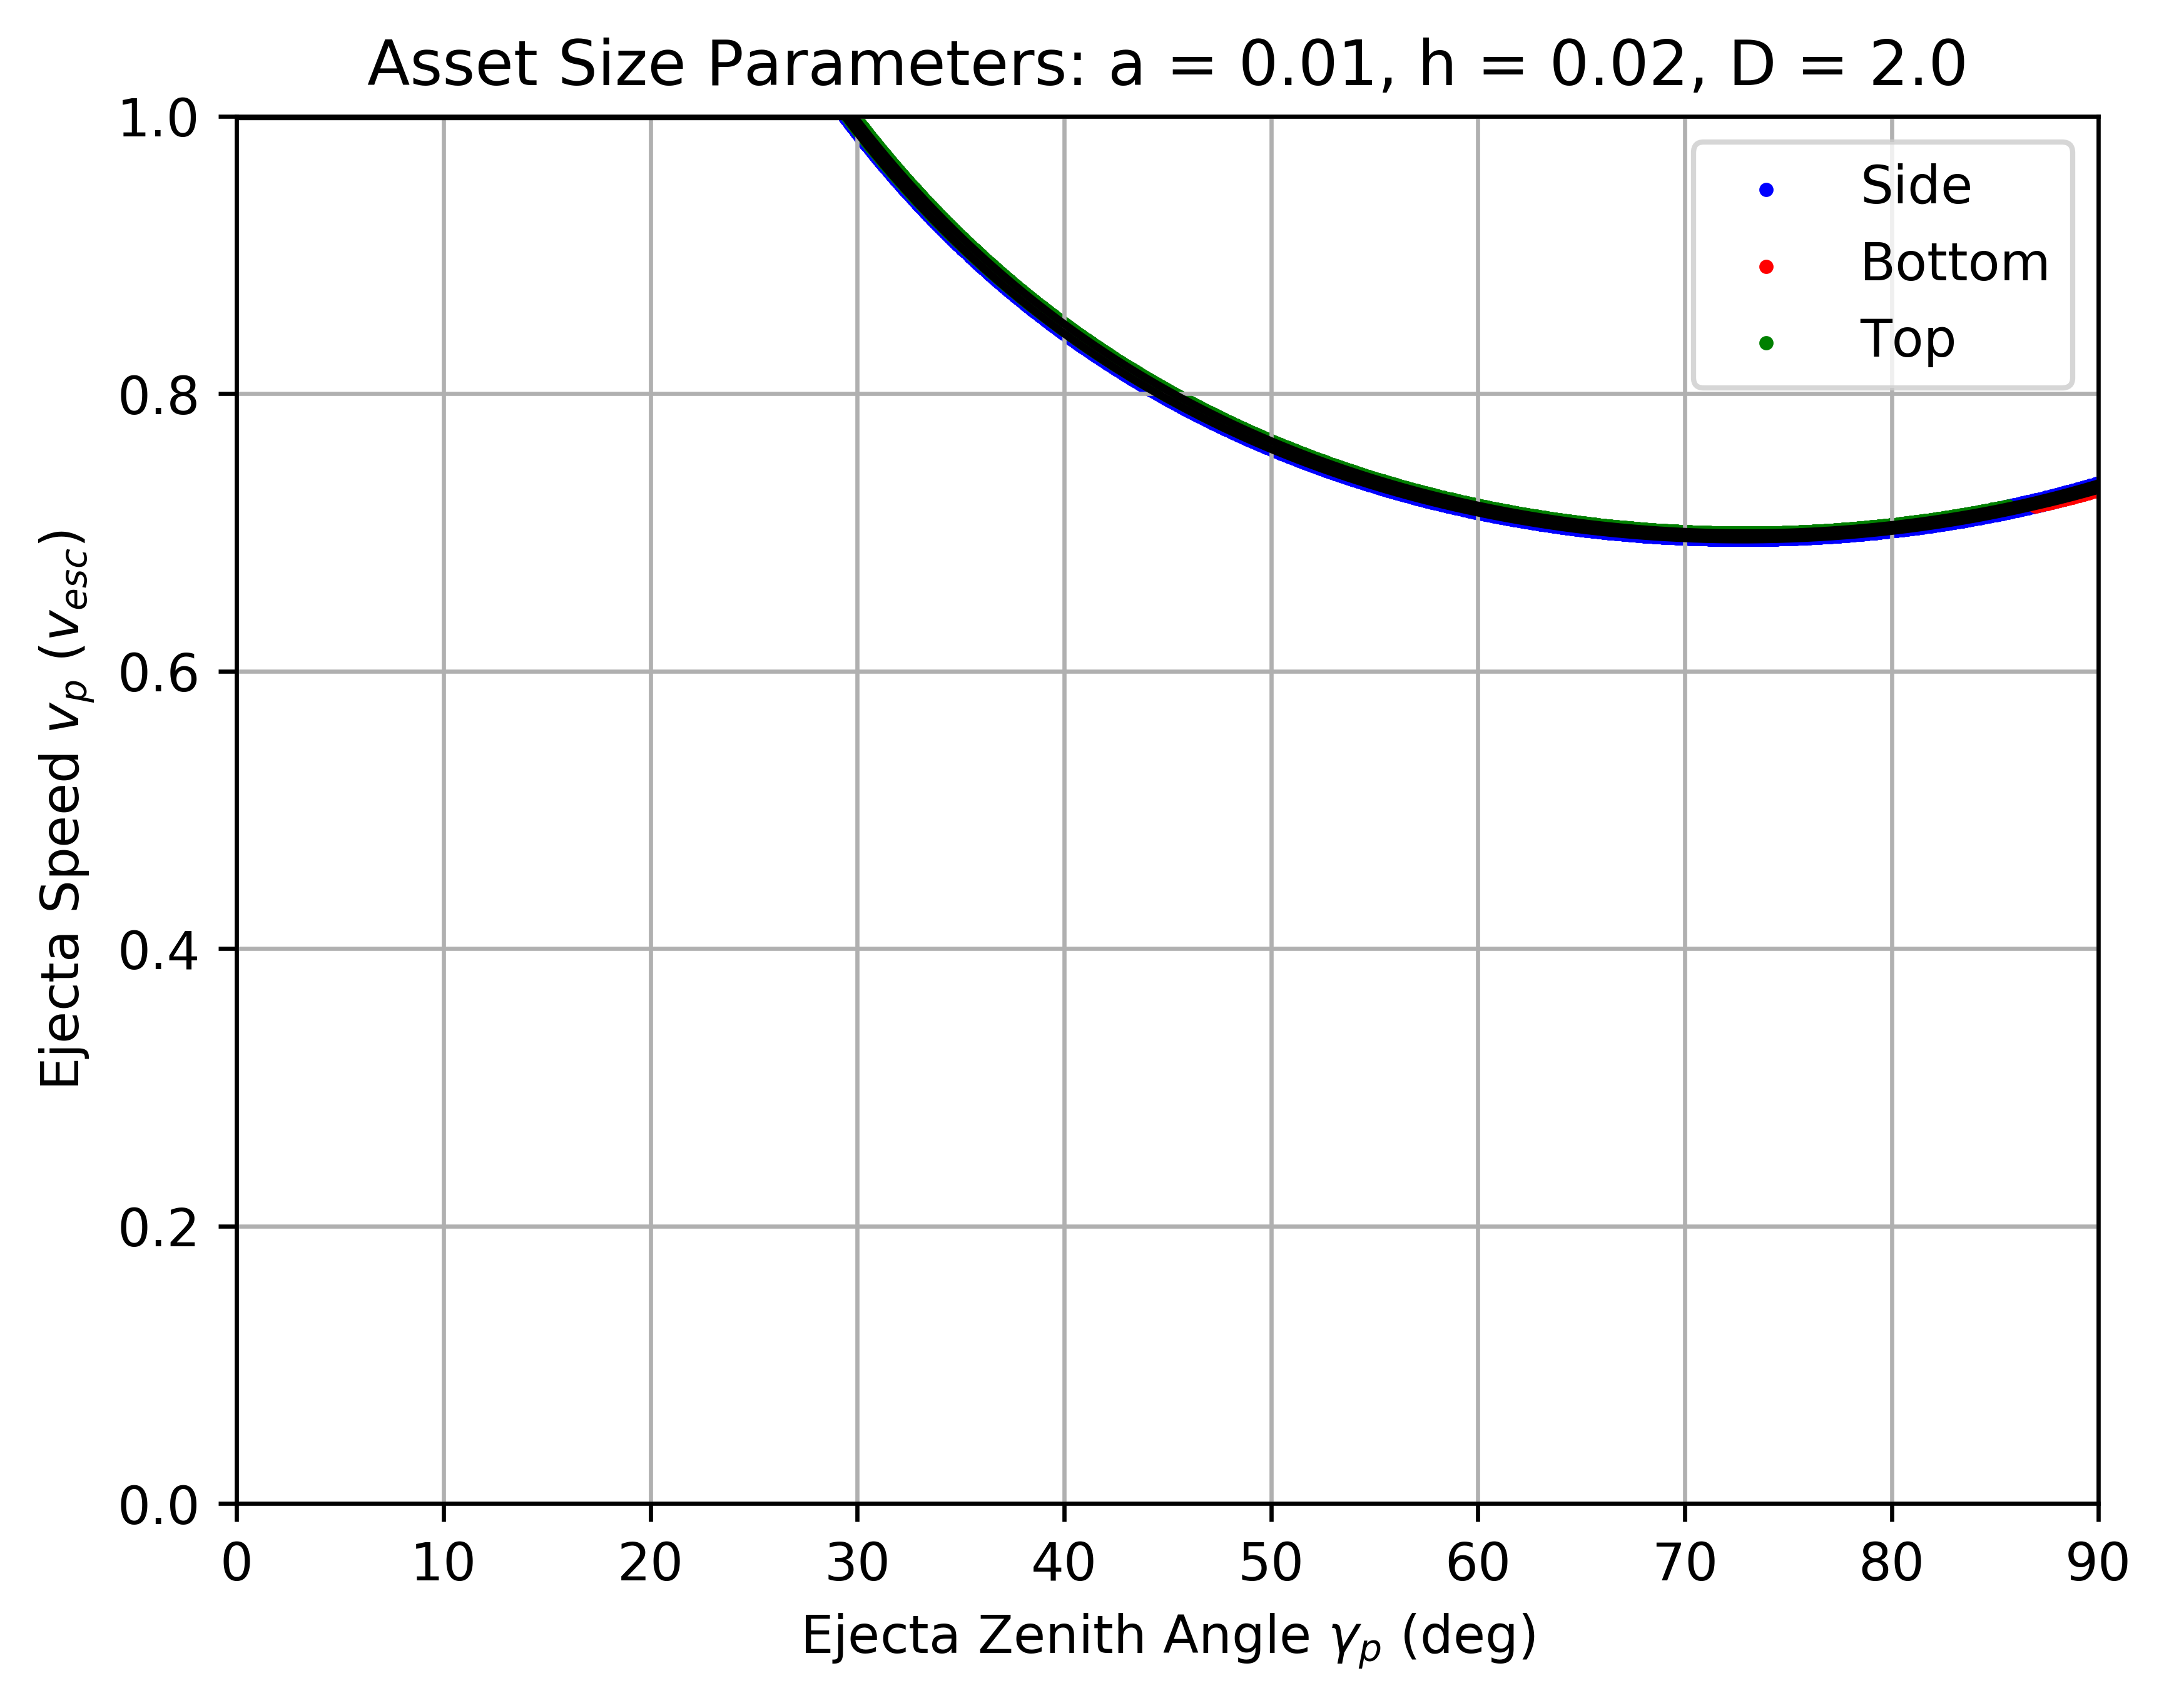
\includegraphics[width=.98\linewidth]{asset_speed_zenith_plot_1.100e+00_1.000e-02_2.000e-02_2.000e+00.png}  
		%\caption{Put your sub-caption here}
		\label{fig:sub-asset_speed_zenith_h2_11}
	\end{subfigure}
	\begin{subfigure}[t]{.32\textwidth}
		\centering
		% include fourth image
		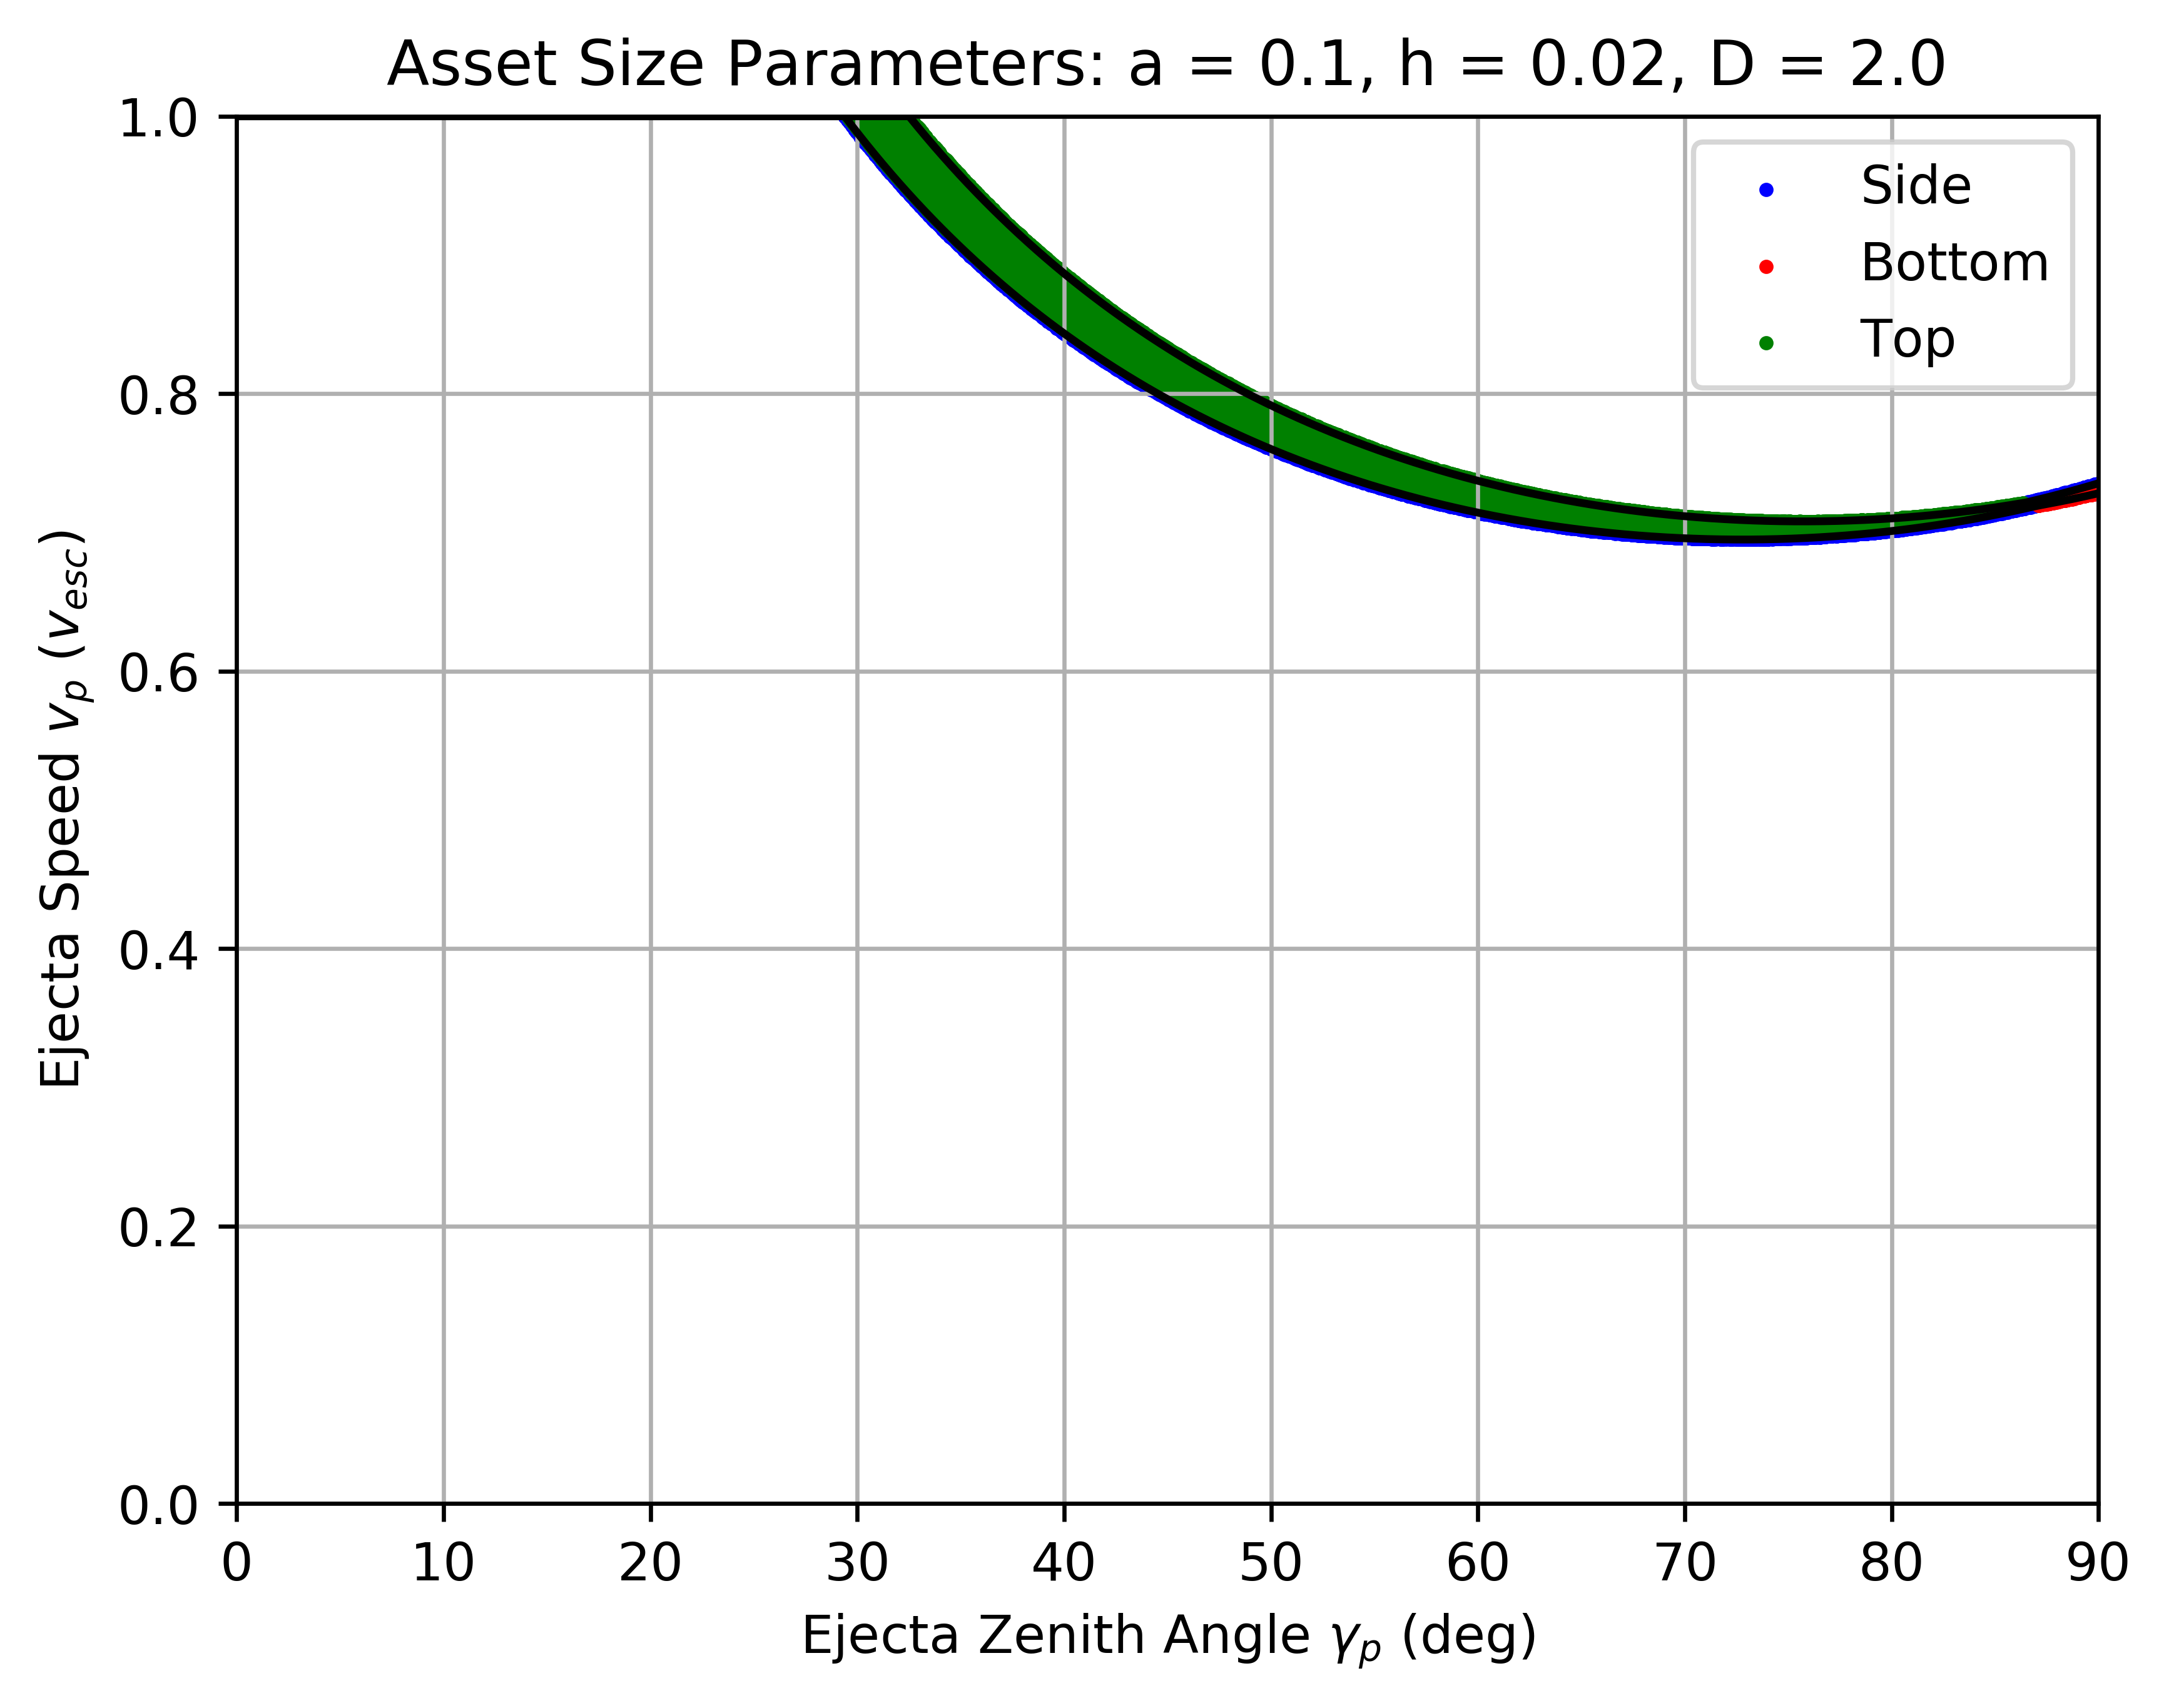
\includegraphics[width=.98\linewidth]{asset_speed_zenith_plot_1.100e+00_1.000e-01_2.000e-02_2.000e+00.png}  
		%\caption{Put your sub-caption here}
		\label{fig:sub-asset_speed_zenith_h2_12}
	\end{subfigure}
	
	\caption{A matrix of plots showing the ejecta hitting a cylindrical asset (in a plane intersecting the cylinder's symmetry axis) with a height above the surface of $0.1 r_m$ for various asset sizes and crater-to-asset distances. Each plot gives three colors for the ejecta hitting the side (blue), bottom (red), and the top (green) as a function of initial ejecta speed $v_p$ vs.\ initial ejecta zenith angle $\gamma_p$.}
	\label{fig:asset_speed_zenith_comparison_h2}
\end{figure}

\clearpage

%%%%%%%%%%%%%%%%%%%%%%%%%%%%%%%%%%%%%%%%%%%%%%%%%%%%%%%%%%%%%%%%%%%%%%
\subsection{Ejecta Speed-Zenith-Azimuth Sampling Algorithm}\label{ssec:Ejecta Speed-Zenith-Azimuth Sampling Algorithm}
There are two integration techniques that will combined in order to sample the ejecta speed-zenith phase space, importance sampling \citep[e.g., Section 9.7 of][]{kroese2013handbook} and stratified sampling \citep[e.g., Section 9.5 of][]{kroese2013handbook}.

In general, let $I$ be the integral given by
\begin{equation}
I = \int g(x)dx.
\end{equation}

Using importance sampling, the integral $I$ can be approximated as
\begin{equation}
I \sim \frac{1}{n}\sum_{i=1}^{n}\frac{g(x_i)}{f_{\hat{x}}(x_i)},
\end{equation}
where $f_{\hat{x}}(x_i)$ is a probability distribution function close to $g(x)$.

The integral $I$ can also be approximated using stratified sampling as
\begin{equation}
I \sim \sum_{j=1}^{k}\frac{vol(M_j)}{n_j}\sum_{i=1}^{n_j}g(x_{ij}),
\end{equation}
where each subdomain $M_j$ has a volume $vol(M_j)$.

Combining the two integration techniques, the integral $I$ can be written as
\begin{equation}
I \sim \sum_{j=1}^{k}\frac{Vol(M_j)}{n_j}\sum_{i=1}^{n}\frac{g(x_{ij})}{f_{\hat{x}(x_{ij})}}.
\end{equation}


In the case of computing the fraction of total ejecta $M$ that hits the asset from a particular crater $\mathcal{C}$, the integral $I$ will be assigned as $M$ such that
\begin{equation}
M(\mathcal{C}) = \frac{1}{2\pi}\int_{\mathcal{R}(v_p,\gamma_p, \beta_i), \Phi(\beta_i)} d\beta_i d\gamma_p dv \frac{dM(v_p,\gamma_p)}{dv} F(\gamma_p) G(\beta_i-\beta_{imp}),
\end{equation}
where examples of the region $\mathcal{R}(v_p,\gamma_p, \beta_i)$ are shown in Figures \ref{fig:asset_speed_zenith_comparison}, \ref{fig:asset_speed_zenith_comparison_h1}, and \ref{fig:asset_speed_zenith_comparison_h2}, $\frac{dM(v_p,\gamma_p)}{dv}$ is the differential of the total ejecta mass (i.e., the differential of Equation~\eqref{eq:M_HH11}), $F(\gamma_p)$ is the ejecta zenith distribution (see Section \ref{sssec:Ejecta:Zenith Distribution}), and $G(\beta_i-\beta_{imp})$ is the ejecta azimuth distribution (see Section \ref{sssec:Ejecta:Azimuth Distribution}) with $\beta_{imp}$ as the impactor azimuth.





\end{document}
\documentclass{article}
\usepackage{amsmath}
\usepackage{graphicx}

\begin{document}

\section{Scaling Laws}\label{sec:Scaling Laws}
The scaling laws used in this model are from \cite{housen2011ejecta}, which assume point-source crater evolution that applies to the final crater size, the growth of the transient crater and the majority of the observable ejecta field.

Depending on the size of the impact event, there are two separate cases: the strength regime and the gravity regime, discussed in Section \ref{ssec:Crater Size}. For smaller impacts, the strength regime dominates while for larger impacts, the gravity regime dominates. For materials that do not have a well defined strength (such as dry sand), the gravity regime dominates for all sizes of impacts.


%%%%%%%%%%%%%%%%%%%%%%%%%%%%%%%%%%%%%%%%%%%%%%%%%%%%%%%%%%%%%%%%%%%%%%
\subsection{Crater Size -- Strength \& Gravity Regime}\label{ssec:Crater Size}

The crater radius as determined by the \cite{housen2011ejecta} scaling laws is computed for both the strength and the gravity regime as the following:
\begin{equation}\label{eq:R gravity}
R\left(\frac{\rho}{m}\right)^{1/3} = H_2\left(\frac{\rho}{\delta}\right)^{\frac{1-3\nu}{3}}\left[\frac{Y}{\rho U^2}\right]^{-\frac{\mu}{2}},
\end{equation}
for the strength regime with $R$ the crater radius, $\rho$ the target bulk density, $m$ the impactor mass, $\delta$ the impactor bulk density, $Y$ the material strength (shear for granular targets and tensile for solid targets), and $U$ the normal component\footnote{See Section 5.2 of \cite{housen2011ejecta}.} of the impactor speed. See Table \ref{tab:scaling law parameters} for various scaling law parameters, and
\begin{equation}\label{eq:R strength}
R\left(\frac{\rho}{m}\right)^{1/3} = H_1\left(\frac{\rho}{\delta}\right)^{\frac{2+\mu-6\nu}{3(2+\mu)}}\left[\frac{ga}{U^2}\right]^{-\frac{\mu}{2+\mu}},
\end{equation}
for the gravity regime with $g = GM/r_m^2 = 1.625$ m s$^{-2}$ the lunar surface gravity, and $a$ the impactor radius.  

%%%%%%%%%%%%%%%%%%%%%%%%%%%%%%%%%%%%%%%%%%%%%%%%%%%%%%%%%%%%%%%%%%%%%%%
%\subsection{Minimum \& Maximum Ejected Speed}\label{ssec:Min Max Ejecta Speed}
%
%%%%%%%%%%%%%%%%%%%%%%%%%%%%%%%%%%%%%%%%%%%%%%%%%%%%%%%%%%%%%%%%%%%%%%%
%\subsection{Maximum Ejected Particle Mass}

%%%%%%%%%%%%%%%%%%%%%%%%%%%%%%%%%%%%%%%%%%%%%%%%%%%%%%%%%%%%%%%%%%%%%%
\subsection{Mass Ejected from Crater}\label{ssec:Mass Ejected from Crater}

The mass ejected from a crater by an impact can be summarized into two equations parameterized by the position from the crater center $x$ as
\begin{align}\label{eq:v/U}
\frac{v}{U} &= C_1\left[\frac{x}{a}\left(\frac{\rho}{\delta}\right)^\nu\right]^{-\frac{1}{\mu}}\left(1 - \frac{x}{n_2 R}\right)^p,\\
\frac{M}{m} &= \frac{3k}{4\pi}\frac{\rho}{\delta}\left[\left(\frac{x}{a}\right)^3-n_1^3\right],\label{eq:M_HH11}
\end{align}
for $n_1 a \le x \le n_2 R$, where $v$ is the ejecta speed, and $M$ is the mass ejected at speeds equal to or greater than $v$.

The maximum speed occurs when $x = n_1 a$, or very close to ground zero, and is given by
\begin{equation}\label{eq:vmax}
\frac{v_{max}}{U} = C_1\left[n_1\left(\frac{\rho}{\delta}\right)^\nu\right]^{-\frac{1}{\mu}}\left(1 - \frac{n_1 a}{n_2 R}\right)^p.
\end{equation}
If $v_{max} \le 0$, then it is assumed no ejecta was created by the impact.

The total mass ejected is given when $x = n_2 R$,
\begin{equation}\label{eq:Mtot}
\frac{M_{tot}}{m} = \frac{3k}{4\pi}\frac{\rho}{\delta}\left[\left(\frac{n_2 R}{a}\right)^3-n_1^3\right].
\end{equation}
It is equivalent to say that if $M_{tot} \le 0$, then no ejecta was created by the impact.

The differential mass in terms of the speed can be computed using the chain rule as follows:
\begin{equation}\label{eq:dM/dv chain rule}
\frac{dM}{dv} = \frac{dM}{dx}\frac{dx}{dv} = \frac{dM}{dx}\left(\frac{dv}{dx}\right)^{-1}.
\end{equation}
The first term can be calculated from Equation \eqref{eq:M_HH11} such that
\begin{equation}\label{eq:dM/dx}
\frac{dM}{dx} = \frac{9k}{4\pi}\frac{\rho}{\delta}\left(\frac{x}{a}\right)^2\frac{m}{a},
\end{equation}
and the second term from Equation \eqref{eq:v/U}, giving
\begin{equation}\label{eq:dv/dx}
\frac{dv}{dx} = -C_1\left[\frac{x}{a}\left(\frac{\rho}{\delta}\right)^\nu\right]^{-\frac{1}{\mu}}\left(1 - \frac{x}{n_2 R}\right)^p
\frac{1+(\mu p -1)\frac{x}{n_2 R}}{\mu\left(1-\frac{x}{n_2 R}\right)}\frac{U}{x}.
\end{equation}
Therefore, the differential mass is found by taking Equation \eqref{eq:dM/dx} divided by Equation~\eqref{eq:dv/dx} giving
\begin{equation}\label{eq:dM/dv final}
\frac{dM}{dv} = -\frac{9k}{4\pi}\frac{\rho}{\delta}\left(\frac{x}{a}\right)^3\frac{\mu\left(1-\frac{x}{n_2 R}\right)}{1+(\mu p-1)\frac{x}{n_2 R}}\frac{m}{v}.
\end{equation}



%%%%%%%%%%%%%%%%%%%%%%%%%%%%%%%%%%%%%%%%%%%%%%%%%%%%%%%%%%%%%%%%%%%%%%
\subsection{Scaling Law Parameters}\label{ssec:Scaling Law Parameters}
%In the meteoroid ejecta model described in this document, the scaling laws from \cite{housen2011ejecta} are employed. In this section, the parameters of various material types used in fits to the scaling laws are summarized. The specific scaling law equations are discussed in Section \ref{sec:Scaling Laws}.

The various sets of parameters for different target materials are given in Table 3 of \cite{housen2011ejecta} with most of them copied here in Table \ref{tab:scaling law parameters}, with undefined values filled in that are best represented by either solid, semi-solid, or fine material where applicable. If a material has zero strength, the crater scaling is automatically in the gravity regime and there is no strength regime (and no need for $H_2$ to be defined).


\begin{table}[!htb]
	\begin{center}
		\caption{Summary of constants used in the \cite{housen2011ejecta} ejecta model.}
		\label{tab:scaling law parameters}
		\begin{tabular}{l l l l l l l l l}
			\hline
			Curve no.\ & C1    & C2   & C3  & C4   & C5   & C6  & C7  & C8  \\
			\hline
			Target     & Water & Rock & WCB & Sand & Sand & GMS & SFA & PS\\
			Porosity   & $\sim 0$ & $\sim 0$ & $20\%$ & $35\pm 5\%$ & $35\pm 5\%$ & $36\%$ & $45\%$ & $60\%$\\
			$\mu$ & $0.55$ & $0.55$ & $0.46$ & $0.41$ & $0.41$ & $0.45$ & $0.4$ & $0.35$\\
			$C_1$ & $1.5$ & $1.5$ & $0.18$ & $0.55$ & $0.55$ & $1.0$ & $0.55$ & $0.6$ \\
			$k$ & $0.2$ & $0.3$ & $0.3$ & $0.3$ & $0.3$ & $0.5$ & $0.3$ & $0.32$\\ 
			$H_1$ & $0.68$ & $0.68^{*1}$ & $0.5^{*2}$ & $0.59$ & $0.59$ & $0.8$ & $0.59^{*3}$ & $0.59^{*3}$\\
			$H_2$ & -- & $1.2$ & $0.38$ & -- & -- & -- & $0.4$ & $0.81$\\
			$n_{2,G}$ & $1.5$ & $1.5$ & $1.3^{*3}$ & $1.3$ & $1.3$ & $1.3$ & $1.2^{*2}$ & $1.2^{*2}$\\
			$p$ & $0.5$ & $0.5$ & $0.3$ & $0.3$ & $0.3$ & $0.3$ & $0.3$ & $0.2$\\
			$Y$ (MPa) & $0$ & $30$ & $0.45$ & $0$ & $0$ & $0$ & $4\times 10^{-3}$ & $2\times 10^{-3}$\\
			\hline
			\multicolumn{9}{l}{\footnotesize Note: WCB = weakly cemented basalt, GMS = glass micro-spheres, PS = perlite/sand mixture,} \\
			\multicolumn{9}{l}{\footnotesize SFA = sand/fly ash. All cases shown in this table used: $\nu=0.4$, $n_1=1.2$, $n_{2,S} = 1$, $g=9.81$ m/s$^2$.} \\
			\multicolumn{9}{l}{\footnotesize $*1$ from water, $*2$ no value given, $*3$ from sand.}\\
			
		\end{tabular}
	\end{center}
\end{table}

The average regolith porosity from $0$ -- $60$ cm is $46\pm 2 \%$ (see Table \ref{tab:porosity}), so the set of parameters that define SFA (sand/fly ash) are adopted. For a higher fidelity strength, Equation \eqref{eq:shear strength_avg_para} can be used instead of $Y = 4$ kPa.





\end{document}
\documentclass{article}
\usepackage{amsmath}
\usepackage{graphicx}

\begin{document}

\section{Secondary Environment at Asset}\label{sec:Secondary Environment}


%%%%%%%%%%%%%%%%%%%%%%%%%%%%%%%%%%%%%%%%%%%%%%%%%%%%%%%%%%%%%%%%%%%%%%
\subsection{Latitude-Longitude Dependence}\label{ssec:env:Latitude-Longitude Dependence}

%%%%%%%%%%%%%%%%%%%%%%%%%%%%%%%%%%%%%%%%%%%%%%%%%%%%%%%%%%%%%%%%%%%%%%
\subsection{Speed Distribution}\label{ssec:env:Speed Distribution}

%%%%%%%%%%%%%%%%%%%%%%%%%%%%%%%%%%%%%%%%%%%%%%%%%%%%%%%%%%%%%%%%%%%%%%
\subsection{Angular Distribution}\label{ssec:env:Angular Distribution}

%%%%%%%%%%%%%%%%%%%%%%%%%%%%%%%%%%%%%%%%%%%%%%%%%%%%%%%%%%%%%%%%%%%%%%
\subsection{Ejecta Size Distribution}\label{ssec:env:Ejecta Size Distribution}



\end{document}




%%%%%%%%%%%%%%%%%%%%%%%%%%%%%%%%%%%%%%%%%%%%%%%%%%%%%%%%%%%%%%%%%%

%\section{References}
\cleardoublepage
\phantomsection
\addcontentsline{toc}{section}{References}
\bibliographystyle{agu}
\bibliography{report}

\end{document}